%% abtex2-modelo-trabalho-academico.tex, v-1.9.2 laurocesar
%% Copyright 2012-2014 by abnTeX2 group at http://abntex2.googlecode.com/ 
%%
%% This work may be distributed and/or modified under the
%% conditions of the LaTeX Project Public License, either version 1.3
%% of this license or (at your option) any later version.
%% The latest version of this license is in
%%   http://www.latex-project.org/lppl.txt
%% and version 1.3 or later is part of all distributions of LaTeX
%% version 2005/12/01 or later.
%%
%% This work has the LPPL maintenance status `maintained'.
%% 
%% The Current Maintainer o	f this work is the abnTeX2 team, led
%% by Lauro César Araujo. Further information are available on 
%% http://abntex2.googlecode.com/
%%
%% This work consists of the files abntex2-modelo-trabalho-academico.tex,
%% abntex2-modelo-include-comandos and abntex2-modelo-references.bib
%%

% ------------------------------------------------------------------------
% ------------------------------------------------------------------------
% abnTeX2: Modelo de Trabalho Academico (tese de doutorado, dissertacao de
% mestrado e trabalhos monograficos em geral) em conformidade com 
% ABNT NBR 14724:2011: Informacao e documentacao - Trabalhos academicos -
% Apresentacao
% ------------------------------------------------------------------------
% ------------------------------------------------------------------------

%-------------------------------------------------------------------------
% Modelo adaptado especificamente para o contexto do PPgSI-EACH-USP por 
% Marcelo Fantinato, com auxílio dos Professores Norton T. Roman, Helton
% H. Bíscaro e Sarajane M. Peres, em 2015, com muitos agradecimentos aos 
% criadores da classe e do modelo base.
%
% 20/06/2017: inclusão de "lista de quadros" com base no especificado em:
% https://github.com/abntex/abntex2/wiki/HowToCriarNovoAmbienteListing,
% de autoria de "Eduardo de Santana Medeiros Alexandre".
%
%-------------------------------------------------------------------------

\documentclass[
	% -- opções da classe memoir --
	12pt,				% tamanho da fonte
	% openright,			% capítulos começam em pág ímpar (insere página vazia caso preciso)
	oneside,			% para impressão apenas no anverso (apenas frente). Oposto a twoside
	a4paper,			% tamanho do papel. 
	% -- opções da classe abntex2 --
	%chapter=TITLE,		% títulos de capítulos convertidos em letras maiúsculas
	%section=TITLE,		% títulos de seções convertidos em letras maiúsculas
	%subsection=TITLE,	% títulos de subseções convertidos em letras maiúsculas
	%subsubsection=TITLE,% títulos de subsubseções convertidos em letras maiúsculas
	% -- opções do pacote babel --
	english,			% idioma adicional para hifenização
	%french,				% idioma adicional para hifenização
	%spanish,			% idioma adicional para hifenização
	brazil				% o último idioma é o principal do documento
	]{abntex2ppgsi}

% ---
% Pacotes básicos 
% ---
% \usepackage{lmodern}			% Usa a fonte Latin Modern			
% \usepackage[T1]{fontenc}		% Selecao de codigos de fonte.
\usepackage[utf8]{inputenc}		% Codificacao do documento (conversão automática dos acentos)
\usepackage{lastpage}			% Usado pela Ficha catalográfica
\usepackage{indentfirst}		% Indenta o primeiro parágrafo de cada seção.
\usepackage{array,booktabs}
\usepackage[pdftex,dvipsnames]{xcolor} 
\usepackage{makecell}
\renewcommand\theadalign{bc}
\renewcommand\theadfont{\bfseries}
\renewcommand\theadgape{\Gape[4pt]}
\renewcommand\cellgape{\Gape[4pt]}
\usepackage{color}				% Controle das cores
\usepackage{graphicx}			% Inclusão de gráficos
\usepackage{microtype} 			% para melhorias de justificação
\usepackage{pdfpages}     %para incluir pdf
\usepackage{algorithm}			%para ilustrações do tipo algoritmo
\usepackage{mdwlist}			%para itens com espaço padrão da abnt
\usepackage[noend]{algpseudocode}			%para ilustrações do tipo algoritmo
\usepackage{amsmath}
\usepackage[flushleft]{threeparttable}
\usepackage{bm}
\usepackage{nomencl}

\usepackage{bera}% optional: just to have a nice mono-spaced font
\usepackage{listings}
\lstset{%
        inputencoding=utf8,
        extendedchars=true,
        literate=%
        {é}{{\'{e}}}1
        {è}{{\`{e}}}1
        {ê}{{\^{e}}}1
        {ë}{{\¨{e}}}1
        {É}{{\'{E}}}1
        {Ê}{{\^{E}}}1
        {û}{{\^{u}}}1
        {ù}{{\`{u}}}1
        {ú}{{\'{u}}}1
        {â}{{\^{a}}}1
        {à}{{\`{a}}}1
        {á}{{\'{a}}}1
        {ã}{{\~{a}}}1
        {Á}{{\'{A}}}1
        {Â}{{\^{A}}}1
        {Ã}{{\~{A}}}1
        {ç}{{\c{c}}}1
        {Ç}{{\c{C}}}1
        {õ}{{\~{o}}}1
        {ó}{{\'{o}}}1
        {ô}{{\^{o}}}1
        {Õ}{{\~{O}}}1
        {Ó}{{\'{O}}}1
        {Ô}{{\^{O}}}1
        {î}{{\^{i}}}1
        {Î}{{\^{I}}}1
        {í}{{\'{i}}}1
        {Í}{{\~{Í}}}1
}
\usepackage{xcolor}
\usepackage{gensymb}
\colorlet{punct}{red!60!black}
\definecolor{background}{HTML}{FFFFFF}
\definecolor{delim}{RGB}{20,105,176}
\colorlet{numb}{magenta!60!black}

\lstdefinelanguage{json}{
    basicstyle=\normalfont\ttfamily,
    numbers=left,
    numberstyle=\scriptsize,
    stepnumber=1,
    numbersep=8pt,
    showstringspaces=false,
    breaklines=true,
    frame=lines,
    backgroundcolor=\color{background},
    literate=
     *
      {:}{{{\color{punct}{:}}}}{1}
      {,}{{{\color{punct}{,}}}}{1}
      {\{}{{{\color{delim}{\{}}}}{1}
      {\}}{{{\color{delim}{\}}}}}{1}
      {[}{{{\color{delim}{[}}}}{1}
      {]}{{{\color{delim}{]}}}}{1}
      {é}{{\'{e}}}1
        {è}{{\`{e}}}1
        {ê}{{\^{e}}}1
        {ë}{{\¨{e}}}1
        {É}{{\'{E}}}1
        {Ê}{{\^{E}}}1
        {û}{{\^{u}}}1
        {ù}{{\`{u}}}1
        {ú}{{\'{u}}}1
        {â}{{\^{a}}}1
        {à}{{\`{a}}}1
        {á}{{\'{a}}}1
        {ã}{{\~{a}}}1
        {Á}{{\'{A}}}1
        {Â}{{\^{A}}}1
        {Ã}{{\~{A}}}1
        {ç}{{\c{c}}}1
        {Ç}{{\c{C}}}1
        {õ}{{\~{o}}}1
        {ó}{{\'{o}}}1
        {ô}{{\^{o}}}1
        {Õ}{{\~{O}}}1
        {Ó}{{\'{O}}}1
        {Ô}{{\^{O}}}1
        {î}{{\^{i}}}1
        {Î}{{\^{I}}}1
        {í}{{\'{i}}}1
        {Í}{{\~{Í}}}1
        {º}{{\degree}}1
}
		
% ---
% Pacotes adicionais, usados apenas no âmbito do Modelo Canônico do abnteX2
% ---
\usepackage{lipsum}				% para geração de dummy text
% ---

% ---
% Pacotes de citações
% ---
\usepackage[brazilian,hyperpageref]{backref}	 % Paginas com as citações na bibl
\usepackage[alf]{abntex2cite}	% Citações padrão ABNT
\usepackage{longtable}

\usepackage{todonotes}
\usepackage{lipsum}                     % Dummytext
\usepackage{xargs}                      % Use more than one optional 
\interfootnotelinepenalty=10000 %% Completely prevent breaking of footnotes


% --- 
% CONFIGURAÇÕES DE PACOTES
% --- 

% ---
% Configurações do pacote backref
% Usado sem a opção hyperpageref de backref
\renewcommand{\backrefpagesname}{Citado na(s) página(s):~}
% Texto padrão antes do número das páginas
\renewcommand{\backref}{}
% Define os textos da citação
\renewcommand*{\backrefalt}[4]{
	\ifcase #1 %
		Nenhuma citação no texto.%
	\or
		Citado na página #2.%
	\else
		Citado #1 vezes nas páginas #2.%
	\fi}%
	
\newcommandx{\unsure}[2][1=]{\todo[linecolor=red,backgroundcolor=red!25,bordercolor=red,#1]{#2}}
\newcommandx{\change}[2][1=]{\todo[linecolor=blue,backgroundcolor=blue!25,bordercolor=blue,#1]{#2}}
\newcommandx{\info}[2][1=]{\todo[linecolor=OliveGreen,backgroundcolor=OliveGreen!25,bordercolor=OliveGreen,#1]{#2}}
\newcommandx{\improvement}[2][1=]{\todo[linecolor=Plum,backgroundcolor=Plum!25,bordercolor=Plum,#1]{#2}}
\newcommandx{\thiswillnotshow}[2][1=]{\todo[disable,#1]{#2}}
% ---

% ---
% Informações de dados para CAPA e FOLHA DE ROSTO
% ---

%-------------------------------------------------------------------------
% Comentário adicional do PPgSI - Informações sobre o ``instituicao'':
%
% Não mexer. Deixar exatamente como está.
%
%-------------------------------------------------------------------------
\instituicao{
	UNIVERSIDADE DE SÃO PAULO
	\par
	ESCOLA DE ARTES, CIÊNCIAS E HUMANIDADES
	\par
	PROGRAMA DE PÓS-GRADUAÇÃO EM SISTEMAS DE INFORMAÇÃO}

%-------------------------------------------------------------------------
% Comentário adicional do PPgSI - Informações sobre o ``título'':
%
% Em maiúscula apenas a primeira letra da sentença (do título), exceto 
% nomes próprios, geográficos, institucionais ou Programas ou Projetos ou 
% siglas, os quais podem ter letras em maiúscula também.
%
% O subtítulo do trabalho é opcional.
% Sem ponto final.
%
% Atenção: o título da Dissertação na versão corrigida não pode mudar. 
% Ele deve ser idêntico ao da versão original.
%
%-------------------------------------------------------------------------
\titulo{Caracterização de eventos de exceção e de seus respectivos impactos no sistema de transporte público por ônibus da cidade de São Paulo}

%-------------------------------------------------------------------------
% Comentário adicional do PPgSI - Informações sobre o ``autor'':
%
% Todas as letras em maiúsculas.
% Nome completo.
% Sem ponto final.
%-------------------------------------------------------------------------
\autor{\uppercase{Felipe Cordeiro Alves Dias}}

%-------------------------------------------------------------------------
% Comentário adicional do PPgSI - Informações sobre o ``local'':
%
% Não incluir o ``estado''.
% Sem ponto final.
%-------------------------------------------------------------------------
\local{São Paulo}

%-------------------------------------------------------------------------
% Comentário adicional do PPgSI - Informações sobre a ``data'':
%
% Colocar o ano do depósito (ou seja, o ano da entrega) da respectiva 
% versão, seja ela a versão original (para a defesa) seja ela a versão 
% corrigida (depois da aprovação na defesa). 
%
% Atenção: Se a versão original for depositada no final do ano e a versão 
% corrigida for entregue no ano seguinte, o ano precisa ser atualizado no 
% caso da versão corrigida. 
% Cuidado, pois o ano da ``capa externa'' também precisa ser atualizado 
% nesse caso.
%
% Não incluir o dia, nem o mês.
% Sem ponto final.
%-------------------------------------------------------------------------
\data{2017}

%-------------------------------------------------------------------------
% Comentário adicional do PPgSI - Informações sobre o ``Orientador'':
%
% Se for uma professora, trocar por ``Profa. Dra.''
% Nome completo.
% Sem ponto final.
%-------------------------------------------------------------------------
\orientador{Prof. Dr. Daniel de  Angelis Cordeiro}

%-------------------------------------------------------------------------
% Comentário adicional do PPgSI - Informações sobre o ``Coorientador'':
%
% Opcional. Incluir apenas se houver co-orientador formal, de acordo com o 
% Regulamento do Programa.
%
% Se for uma professora, trocar por ``Profa. Dra.''
% Nome completo.
% Sem ponto final.
%-------------------------------------------------------------------------
%\coorientador{Prof. Dr. Fulano de Tal}

\tipotrabalho{Qualificação (Mestrado)}

\preambulo{
%-------------------------------------------------------------------------
% Comentário adicional do PPgSI - Informações sobre o texto ``Versão 
% original'':
%
% Não usar para Qualificação.
% Não usar para versão corrigida de Dissertação.
%
%-------------------------------------------------------------------------
Versão original \newline \newline \newline 
%-------------------------------------------------------------------------
% Comentário adicional do PPgSI - Informações sobre o ``texto principal do
% preambulo'':
%
Texto de Exame de Qualificação apresentado à Escola de Artes, Ciências e Humanidades da Universidade de São Paulo como parte dos requisitos para obtenção do título de Mestre em Ciências pelo Programa de Pós-graduação em Sistemas de Informação.
%
%-------------------------------------------------------------------------
%Dissertação apresentada à Escola de Artes, Ciências e Humanidades da Universidade de São Paulo para obtenção do título de Mestre em Ciências pelo Programa de Pós-graduação em Sistemas de Informação. 
%
\newline \newline Área de concentração: Metodologia e Técnicas da Computação
%-------------------------------------------------------------------------
% Comentário adicional do PPgSI - Informações sobre o texto da ``Versão 
% corrigida'':
%
% Não usar para Qualificação.
% Não usar para versão original de Dissertação.
% 
% Substituir ``xx de xxxxxxxxxxxxxxx de xxxx'' pela ``data da defesa''.
%
%-------------------------------------------------------------------------
%\newline \newline \newline Versão corrigida contendo as alterações solicitadas pela comissão julgadora em xx de xxxxxxxxxxxxxxx de xxxx. A versão original encontra-se em acervo reservado na Biblioteca da EACH-USP e na Biblioteca Digital de Teses e Dissertações da USP (BDTD), de acordo com a Resolução CoPGr 6018, de 13 de outubro de 2011.
}
% ---


% ---
% Configurações de aparência do PDF final

% alterando o aspecto da cor azul
\definecolor{blue}{RGB}{41,5,195}

% informações do PDF
\makeatletter
\hypersetup{
     	%pagebackref=true,
		pdftitle={\@title}, 
		pdfauthor={\@author},
    	pdfsubject={\imprimirpreambulo},
	    pdfcreator={LaTeX com abnTeX2 adaptado para o PPgSI-EACH-USP},
		pdfkeywords={abnt}{latex}{abntex}{abntex2}{qualificação de mestrado}{dissertação de mestrado}{ppgsi}, 
		colorlinks=true,       		% false: boxed links; true: colored links
    	linkcolor=black,          	% color of internal links
    	citecolor=black,        		% color of links to bibliography
    	filecolor=black,      		% color of file links
		urlcolor=black,
		bookmarksdepth=4
}
\makeatother
% --- 

% --- 
% Espaçamentos entre linhas e parágrafos 
% --- 

% O tamanho do parágrafo é dado por:
\setlength{\parindent}{1.25cm}

% Controle do espaçamento entre um parágrafo e outro:
\setlength{\parskip}{0cm}  % tente também \onelineskip
\renewcommand{\baselinestretch}{1.5}

% ---
% compila o indice
% ---
\makeindex
% ---

	% Controlar linhas orfas e viuvas
  \clubpenalty10000
  \widowpenalty10000
  \displaywidowpenalty10000

% ----
% Início do documento
% ----
\begin{document}

% Retira espaço extra obsoleto entre as frases.
\frenchspacing 

% ----------------------------------------------------------
% ELEMENTOS PRÉ-TEXTUAIS
% ----------------------------------------------------------
% \pretextual

% ---
% Capa
% ---
%-------------------------------------------------------------------------
% Comentário adicional do PPgSI - Informações sobre a ``capa'':
%
% Esta é a ``capa'' principal/oficial do trabalho, a ser impressa apenas 
% para os casos de encadernação simples (ou seja, em ``espiral'' com 
% plástico na frente).
% 
% Não imprimir esta ``capa'' quando houver ``capa dura'' ou ``capa brochura'' 
% em que estas mesmas informações já estão presentes nela.
%
%-------------------------------------------------------------------------
\imprimircapa
% ---

% ---
% Folha de rosto
% (o * indica que haverá a ficha bibliográfica)
% ---
\imprimirfolhaderosto*
% ---

% ---
% Inserir a autorização para reprodução e ficha bibliografica
% ---

%-------------------------------------------------------------------------
% Comentário adicional do PPgSI - Informações sobre o texto da 
% ``autorização para reprodução e ficha bibliografica'':
%
% Página a ser usada apenas para Dissertação (tanto na versão original 
% quanto na versão corrigida).
%
% Solicitar a ficha catalográfica na Biblioteca da EACH. 
% Duas versões devem ser solicitadas, em dois momentos distintos: uma vez 
% para a versão original, e depois outra atualizada para a versão 
% corrigida.
%
% Atenção: esta página de ``autorização para reprodução e ficha 
% catalográfica'' deve ser impressa obrigatoriamente no verso da folha de 
% rosto.
%
% Não usar esta página para Qualificação.
%
% Substitua o arquivo ``fig_ficha_catalografica.pdf'' abaixo referenciado 
% pelo PDF elaborado pela Biblioteca
%
%-------------------------------------------------------------------------
%\begin{fichacatalografica}
%    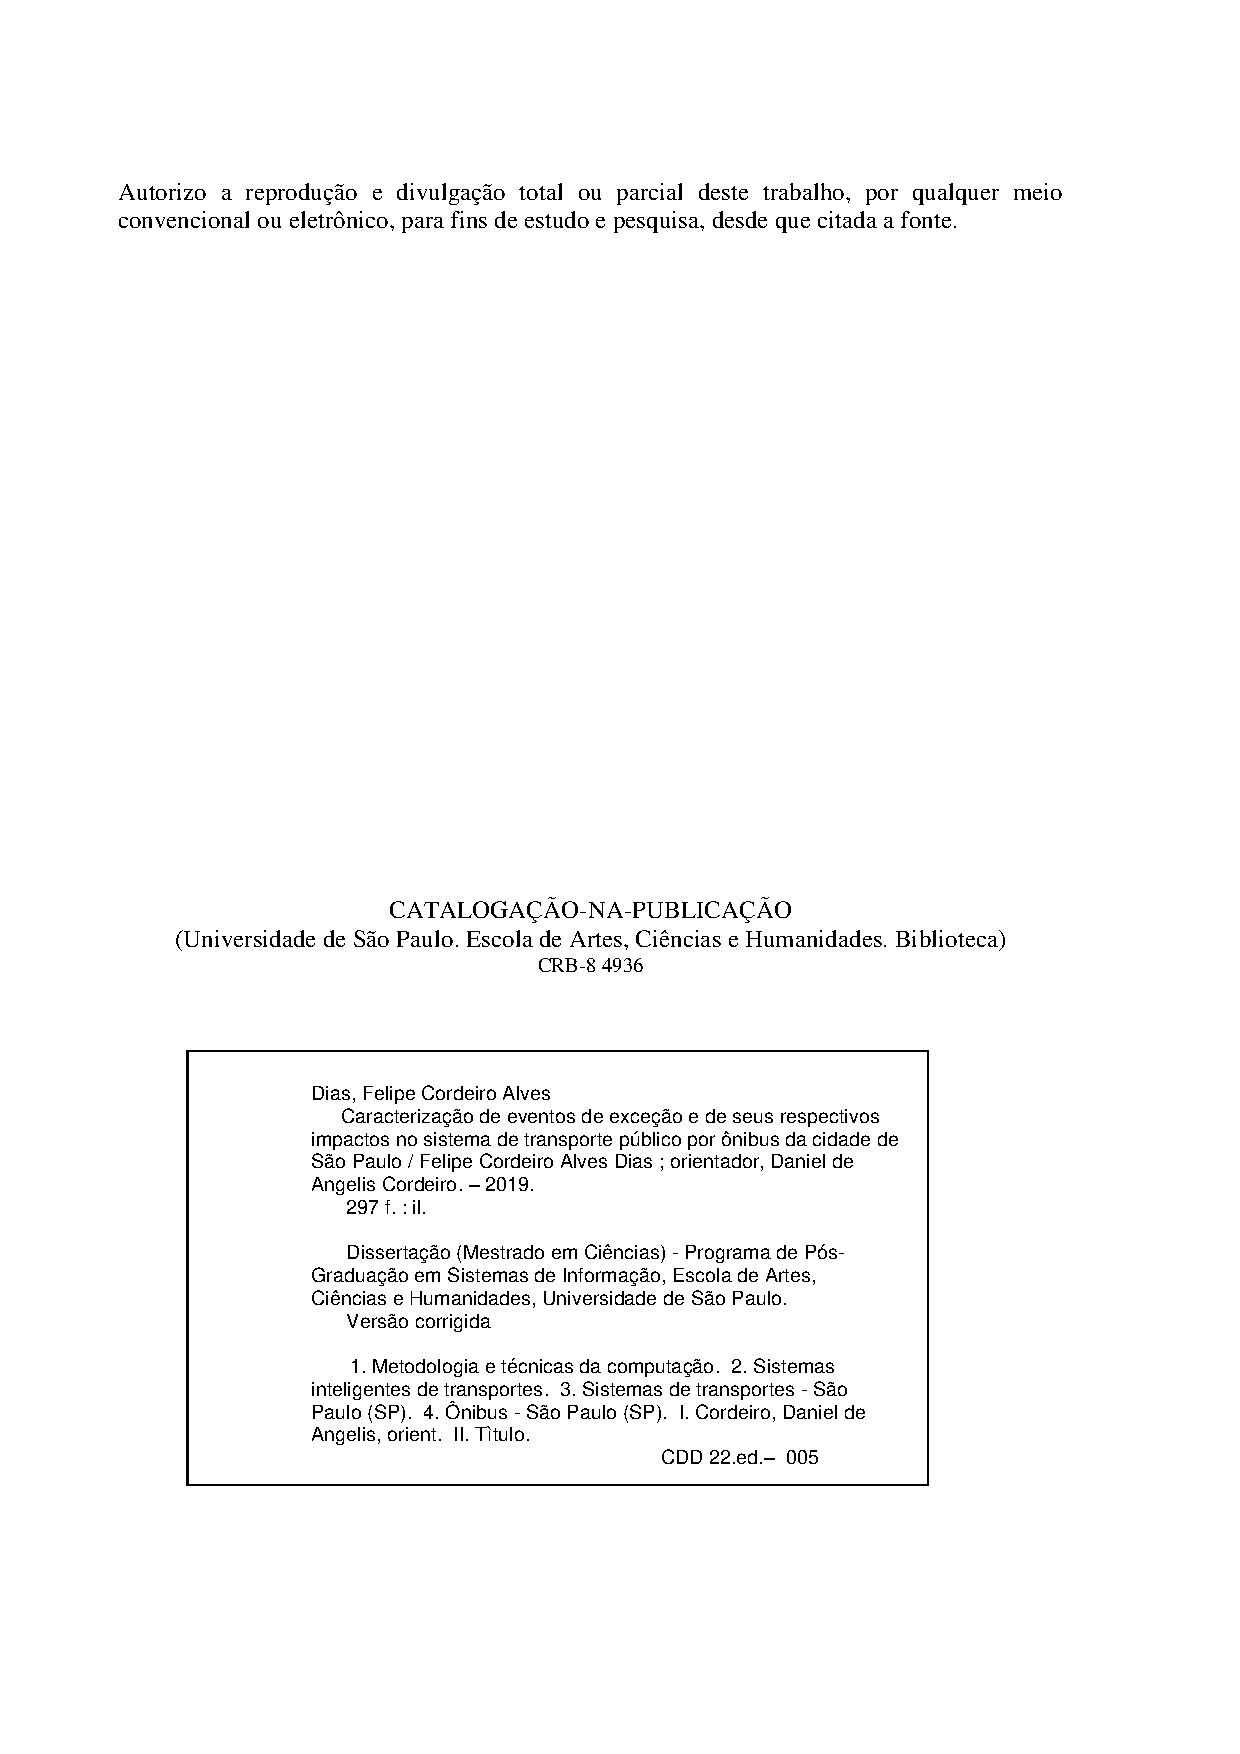
\includepdf{fig_ficha_catalografica.pdf}
%\end{fichacatalografica}

% ---
% Inserir errata
% ---
%-------------------------------------------------------------------------
% Comentário adicional do PPgSI - Informações sobre ``Errata'':
%
% Usar esta página de errata apenas em casos de excepcionais, e apenas 
% para a versão corrigida da Dissertação. Por exemplo, quando depois de
% já depositada e publicada a versão corrigida, ainda assim verifica-se
% a necessidade de alguma correção adicional.
%
% Se precisar usar esta página, busque a forma correta (o modelo correto) 
% para fazê-lo, de acordo com a norma ABNT.
%
% Não usar esta página para versão original de Dissertação.
% Não usar esta página para Qualificação.
%
%-------------------------------------------------------------------------
%\begin{errata}
%Elemento opcional para versão corrigida, depois de depositada.
%\end{errata}
% ---

% ---
% Inserir folha de aprovação
% ---

%\begin{folhadeaprovacao}
%-------------------------------------------------------------------------
% Comentário adicional do PPgSI - Informações sobre ``Folha da aprovação'':
%
% Página a ser usada apenas para Dissertação.
%
% Não usar esta página para Qualificação.
%
% Substituir ``Fulano de Tal'' pelo nome completo do autor do trabalho, com 
% apenas as iniciais em maiúsculo.
%
% Substituir ``___ de ______________ de ______'' por: 
%     - Para versão original de Dissertação: deixar em branco, pois a data 
%       pode mudar, mesmo que ela já esteja prevista.
%     - Para versão corrigida de Dissertação: usar a data em que a defesa 
%       efetivamente ocorreu.
%
%-------------------------------------------------------------------------
%\noindent Dissertação de autoria de Fulano de Tal, sob o título \textbf{``\imprimirtitulo''}, apresentada à Escola de Artes, Ciências e Humanidades da Universidade de São Paulo, para obtenção do título de Mestre em Ciências pelo Programa de Pós-graduação em Sistemas de Informação, na área de concentração Metodologia e Técnicas da Computação, aprovada em \_\_\_\_\_\_\_ de \_\_\_\_\_\_\_\_\_\_\_\_\_\_\_\_\_\_\_\_\_\_ de \_\_\_\_\_\_\_\_\_\_ pela comissão julgadora constituída pelos doutores:

%\vspace*{3cm}

%\begin{center}
%-------------------------------------------------------------------------
% Comentário adicional do PPgSI - Informações sobre ``assinaturas'':
%
% Para versão original de Dissertação: deixar em 
% branco (ou seja, assim como está abaixo), pois os membros da banca podem
% mudar, mesmo que eles já estejam previstos.
% 
% Para versão corrigida de Dissertação: usar os dados dos examinadores que 
% efetivamente participaram da defesa. 
% 
% Para versão corrigida de Dissertação: em caso de ``professora'', trocar 
% por ``Profa. Dra.'' 
% 
% Para versão corrigida de Dissertação: ao colocar os nomes dos 
% examinadores, remover o sublinhado
% 
% Para versão corrigida de Dissertação: ao colocar os nomes dos 
% examinadores, usar seus nomes completos, exatamente conforme constam em 
% seus Currículos Lattes
% 
% Para versão corrigida de Dissertação: ao colocar os nomes das 
% instituições, remover o sublinhado e remover a palavra ``Instituição:''
%
% Não abreviar os nomes das instituições.
%
%-------------------------------------------------------------------------
%\_\_\_\_\_\_\_\_\_\_\_\_\_\_\_\_\_\_\_\_\_\_\_\_\_\_\_\_\_\_\_\_\_\_\_\_\_\_\_\_\_\_\_\_\_\_\_\_\_\_\_\_\_\_\_\_
%\vspace*{0.2cm} 
%\\ \textbf{Prof. Dr. %\_\_\_\_\_\_\_\_\_\_\_\_\_\_\_\_\_\_\_\_\_\_\_\_\_\_\_\_\_\_\_\_\_\_\_\_\_\_\_\_\_\_\_\_\_\_\_\_\_\_\_\_\_\_\_\_\_\_\_\_\_\_} 
%\\ \vspace*{0.2cm} 
%Instituição: %\_\_\_\_\_\_\_\_\_\_\_\_\_\_\_\_\_\_\_\_\_\_\_\_\_\_\_\_\_\_\_\_\_\_\_\_\_\_\_\_\_\_\_\_\_\_\_\_\_\_\_\_\_\_\_\_\_\_ 
%\\ \vspace*{0.2cm}
%Presidente 

%\vspace*{2cm}

%\_\_\_\_\_\_\_\_\_\_\_\_\_\_\_\_\_\_\_\_\_\_\_\_\_\_\_\_\_\_\_\_\_\_\_\_\_\_\_\_\_\_\_\_\_\_\_\_\_\_\_\_\_\_\_\_
%\vspace*{0.2cm} 
%\\ \textbf{Prof. Dr. %\_\_\_\_\_\_\_\_\_\_\_\_\_\_\_\_\_\_\_\_\_\_\_\_\_\_\_\_\_\_\_\_\_\_\_\_\_\_\_\_\_\_\_\_\_\_\_\_\_\_\_\_\_\_\_\_\_\_\_\_\_\_} 
%\\ \vspace*{0.2cm} 
%Instituição: %\_\_\_\_\_\_\_\_\_\_\_\_\_\_\_\_\_\_\_\_\_\_\_\_\_\_\_\_\_\_\_\_\_\_\_\_\_\_\_\_\_\_\_\_\_\_\_\_\_\_\_\_\_\_\_\_\_\_

%\vspace*{2cm}

%\_\_\_\_\_\_\_\_\_\_\_\_\_\_\_\_\_\_\_\_\_\_\_\_\_\_\_\_\_\_\_\_\_\_\_\_\_\_\_\_\_\_\_\_\_\_\_\_\_\_\_\_\_\_\_\_
%\vspace*{0.2cm} 
%\\ \textbf{Prof. Dr. %\_\_\_\_\_\_\_\_\_\_\_\_\_\_\_\_\_\_\_\_\_\_\_\_\_\_\_\_\_\_\_\_\_\_\_\_\_\_\_\_\_\_\_\_\_\_\_\_\_\_\_\_\_\_\_\_\_\_\_\_\_\_} 
%\\ \vspace*{0.2cm} 
%Instituição: %\_\_\_\_\_\_\_\_\_\_\_\_\_\_\_\_\_\_\_\_\_\_\_\_\_\_\_\_\_\_\_\_\_\_\_\_\_\_\_\_\_\_\_\_\_\_\_\_\_\_\_\_\_\_\_\_\_\_

%\vspace*{2cm}

%\_\_\_\_\_\_\_\_\_\_\_\_\_\_\_\_\_\_\_\_\_\_\_\_\_\_\_\_\_\_\_\_\_\_\_\_\_\_\_\_\_\_\_\_\_\_\_\_\_\_\_\_\_\_\_\_
%\vspace*{0.2cm} 
%\\ \textbf{Prof. Dr. %\_\_\_\_\_\_\_\_\_\_\_\_\_\_\_\_\_\_\_\_\_\_\_\_\_\_\_\_\_\_\_\_\_\_\_\_\_\_\_\_\_\_\_\_\_\_\_\_\_\_\_\_\_\_\_\_\_\_\_\_\_\_} 
%\\ \vspace*{0.2cm} 
%Instituição: %\_\_\_\_\_\_\_\_\_\_\_\_\_\_\_\_\_\_\_\_\_\_\_\_\_\_\_\_\_\_\_\_\_\_\_\_\_\_\_\_\_\_\_\_\_\_\_\_\_\_\_\_\_\_\_\_\_\_

%\end{center}
  
%\end{folhadeaprovacao}
% ---

% ---
% Dedicatória
% ---
%-------------------------------------------------------------------------
% Comentário adicional do PPgSI - Informações sobre ``Dedicatória'': 
%
% Opcional para Dissertação.
% Não sugerido para Qualificação.
% 
%-------------------------------------------------------------------------
%\begin{dedicatoria}
%   \vspace*{\fill}
%   \centering
%   \noindent
%   \textit{Escreva aqui sua dedicatória, se desejar, ou remova esta página...} 
%	 \vspace*{\fill}
%\end{dedicatoria}
% ---

% ---
% Agradecimentos
% ---
%-------------------------------------------------------------------------
% Comentário adicional do PPgSI - Informações sobre ``Agradecimentos'': 
%
% Opcional para Dissertação.
% Não sugerido para Qualificação.
% 
% Lembrar de agradecer agências de fomento e outras instituições similares.
%
%-------------------------------------------------------------------------
%\begin{agradecimentos}
%\end{agradecimentos}
% ---

% ---
% Epígrafe
% ---
%-------------------------------------------------------------------------
% Comentário adicional do PPgSI - Informações sobre ``Epígrafe'': 
%
% Opcional para Dissertação.
% Não sugerido para Qualificação.
% 
%-------------------------------------------------------------------------
%\begin{epigrafe}
%    \vspace*{\fill}
%	\begin{flushright}
%		\textit{``Escreva aqui uma epígrafe, se desejar, ou remova esta página...''\\
%		(Autor da epígrafe)}
%	\end{flushright}
%\end{epigrafe}
% ---

% ---
% RESUMOS
% ---

% resumo em português
\setlength{\absparsep}{18pt} % ajusta o espaçamento dos parágrafos do resumo
\begin{resumo}

%-------------------------------------------------------------------------
% Comentário adicional do PPgSI - Informações sobre ``referência'':
% 
% Troque os seguintes campos pelos dados de sua Dissertação (mantendo a 
% formatação e pontuação):
%   - SOBRENOME
%   - Nome1
%   - Nome2
%   - Nome3
%   - Título do trabalho: subtítulo do trabalho
%   - AnoDeDefesa
%
% Mantenha todas as demais informações exatamente como estão.
% 
% [Não usar essas informações de ``referência'' para Qualificação]
%
%-------------------------------------------------------------------------
\begin{flushleft}
DIAS, Felipe Cordeiro Alves. \textbf{Caracterização de eventos de exceção e de seus respectivos impactos no sistema de transporte público por ônibus da cidade de São Paulo}. \imprimirdata. \pageref{LastPage} f. Dissertação (Mestrado em Ciências) – Escola de Artes, Ciências e Humanidades, Universidade de São Paulo, São Paulo, 2018.
\end{flushleft}

A cidade de São Paulo é o município mais populoso do Brasil, caracterizado por uma segregação urbana responsável por inúmeros problemas relacionados a mobilidade urbana. As ações atuais para resolver os problemas de mobilidade urbana têm pouco aprofundamento em questões tecnológicas e melhorias dos sistemas computacionais existentes -- como as necessárias ao defasado Sistema Integrado de Monitoramento e Transporte (SIM), utilizado para gestão e monitoramento do transporte público por ônibus de São Paulo. Uma das possíveis melhorias é integrar o SIM às Redes Sociais. Com essa perspectiva de integração, esse trabalho tem como objetivo utilizar \textit{tweets} e dados do SIM na caracterização de eventos de exceção e de seus respectivos impactos no sistema de transporte público por ônibus da cidade de São Paulo. Para alcançar tal objetivo, esse trabalho propõe utilizar \textit{tweets} publicados por instituições governamentais responsáveis por reportar eventos de exceção e dados dos módulos AVL (\textit{Automatic Vehicle Location}) do SIM, responsáveis por rastrear e localizar os ônibus do município. A hipótese é de que é possível identificar e localizar eventos de exceção nos \textit{tweets} por meio de Processamento de Linguagem Natural e Expressão Regular, e correlacionar esses eventos com os dados históricos do SIM.

Palavras-chaves: Cidades Inteligentes. Transporte Público. Sistemas de Transporte Inteligentes. Eventos de exceção.
\end{resumo}

% resumo em inglês
%-------------------------------------------------------------------------
% Comentário adicional do PPgSI - Informações sobre ``resumo em inglês''
% 
% Caso a Qualificação ou a Dissertação inteira seja elaborada no idioma inglês, 
% então o ``Abstract'' vem antes do ``Resumo''.
% 
%-------------------------------------------------------------------------
%\begin{resumo}[Abstract]
%\begin{otherlanguage*}{english}

%-------------------------------------------------------------------------
% Comentário adicional do PPgSI - Informações sobre ``referência em inglês''
% 
% Troque os seguintes campos pelos dados de sua Dissertação (mantendo a 
% formatação e pontuação):
%     - SURNAME
%     - FirstName1
%     - MiddleName1
%     - MiddleName2
%     - Work title: work subtitle
%     - DefenseYear (Ano de Defesa)
%
% Mantenha todas as demais informações exatamente como estão.
%
% [Não usar essas informações de ``referência'' para Qualificação]
%
%-------------------------------------------------------------------------
%\begin{flushleft}
%SURNAME, FirstName MiddleName1 MiddleName2. \textbf{Work title}: work subtitle. \imprimirdata. \pageref{LastPage} p. Dissertation (Master of Science) – School of Arts, Sciences and Humanities, University of São Paulo, São Paulo, DefenseYear. 
%\end{flushleft}

%Write here the English version of your ``Resumo''. Example text, example text, example text, example text, example text, example text, example text, example text, example text, example text, example text, example text, example text, example text, example text, example text, example text, example text, example text, example text, example text, example text, example text, example text, example text, example text, example text, example text, example text, example text, example text, example text, example text, example text, example text, example text, example text, example text, example text, example text, example text, example text, example text, example text, example text, example text, example text.

%Keywords: Keyword1. Keyword2. Keyword3. etc.
%\end{otherlanguage*}
%\end{resumo}

% ---
% ---
% inserir lista de figuras
% ---
\pdfbookmark[0]{\listfigurename}{lof}
\listoffigures*
\cleardoublepage
% ---

% ---
% inserir lista de algoritmos
% ---
%\pdfbookmark[0]{\listalgorithmname}{loa}
%\listofalgorithms
%\cleardoublepage

% ---
% inserir lista de quadros
% ---
%\pdfbookmark[0]{\listofquadrosname}{loq}
%\listofquadros*
%\cleardoublepage


% ---
% inserir lista de tabelas
% ---
\pdfbookmark[0]{\listtablename}{lot}
\listoftables*
\cleardoublepage
% ---

% ---
% inserir lista de abreviaturas e siglas
% ---
%-------------------------------------------------------------------------
% Comentário adicional do PPgSI - Informações sobre ``Lista de abreviaturas 
% e siglas'': 
%
% Opcional.
% Uma vez que se deseja usar, é necessário manter padrão e consistência no
% trabalho inteiro.
% Se usar: inserir em ordem alfabética.
%
%-------------------------------------------------------------------------

% Definicao da lista de abreviaturas e siglas
\renewcommand{\nomname}{Lista de abreviaturas e siglas}
\makenomenclature
\printnomenclature[1in]

\newpage
% ---

% ---
% inserir lista de símbolos
% ---
%-------------------------------------------------------------------------
% Comentário adicional do PPgSI - Informações sobre ``Lista de símbolos'': 
%
% Opcional.
% Uma vez que se deseja usar, é necessário manter padrão e consistência no
% trabalho inteiro.
% Se usar: inserir na ordem em que aparece no texto.
% 
%-------------------------------------------------------------------------
%\begin{simbolos}
%  \item[$ \Gamma $] Letra grega Gama
%  \item[$ \Lambda $] Lambda
%  \item[$ \zeta $] Letra grega minúscula zeta
%  \item[$ \in $] Pertence
%\end{simbolos}
% ---

% ---
% inserir o sumario
% ---
\pdfbookmark[0]{\contentsname}{toc}
\tableofcontents*
\cleardoublepage
% ---



% ----------------------------------------------------------
% ELEMENTOS TEXTUAIS
% ----------------------------------------------------------
\textual


%-------------------------------------------------------------------------
% Comentário adicional do PPgSI - Informações sobre ``títulos de seções''
% 
% Para todos os títulos (seções, subseções, tabelas, ilustrações, etc.):
%
% Em maiúscula apenas a primeira letra da sentença (do título), exceto 
% nomes próprios, geográficos, institucionais ou Programas ou Projetos ou
% siglas, os quais podem ter letras em maiúscula também.
%
%-------------------------------------------------------------------------
\chapter{Introdução}
\label{introducao}

Neste capítulo, são apresentadas as seções
referentes à motivação da proposta de pesquisa; sobre a definição do problema que pretendemos abordar; a respeito dos objetivos gerais e específicos; sobre as hipóteses a serem verificadas e sobre a organização dos capítulos desse documento.

\section{Motivação}
\label{motivation}

A cidade de São Paulo é o município mais populoso do Brasil, que passou por um rápido processo de urbanização e tem população atual estimada em 12.106.920 milhões de habitantes (com data de referência em 1º de julho de 2017)\footnote{\url{https://agenciadenoticias.ibge.gov.br/media/com\_mediaibge/arquivos/9bc1a0065c49fd6f81dc785b2b8d8c35.xlsx}. Acesso em Outubro, 29 de 2017.}.
Desse total de habitantes, 10\% vivem na área do \nomenclature{CE}{Centro Expandido}
{Centro Expandido (CE)} e 90\% no \nomenclature{CP}{­ Cinturão Periférico}{Cinturão Periférico (CP)} \cite{SA201722}, o que caracteriza uma segregação urbana responsável por inúmeros problemas relacionados a mobilidade urbana. 

Um desses problemas é conhecido como o movimento pendular, no qual longas distâncias são percorridas diariamente pelos moradores do CP para acessar os locais de emprego, educação e serviços localizados em maioria no CE. Além disso, o movimento pendular torna o CP  uma região dormitória, com parte de seus respectivos moradores dependentes do Sistema de Transporte Público para acessar o CE.

Devido aos problemas de mobilidade urbana existentes no Brasil, como os da cidade de São Paulo, a Lei Federal 12.587/2012\footnote{\url{http://www.planalto.gov.br/ccivil\_03/\_ato2011-2014/2012/lei/l12587.htm}. Acesso em Outubro, 29 de 2017.}, relacionada ao \nomenclature{PAC}{Programa de Aceleração do Crescimento}{Programa de Aceleração do Crescimento\footnote{\url{http://www.pac.gov.br}. Acesso em Outubro, 29 de 2017.} (PAC),} obrigou os municípios a enviarem seus respectivos planos de mobilidade urbana até o final do ano de 2015, com o objetivo de promover o desenvolvimento sustentável com a mitigação dos custos ambientais e socioeconômicos dos deslocamentos de pessoas. Em resposta a essa lei, o \nomenclature{PlanMob/SP}{Plano de Mobilidade Urbana de São Paulo}{Plano de Mobilidade Urbana de São Paulo (\textit{PlanMob/SP 2015})} foi instituído pelo Decreto 56.834\footnote{\label{planmob}\url{http://www.prefeitura.sp.gov.br/cidade/secretarias/transportes/planmob}. Acesso em Outubro, 29 de 2017.}, como instrumento de planejamento e gestão do Sistema Municipal de Mobilidade Urbana para os próximos 15 anos.

No \textit{PlanMob/SP 2015}, a \nomenclature{SMT}{Secretaria Municipal de Transportes}{Secretaria Municipal de Transportes (SMT)} propõe criar uma central de monitoramento conhecida como \nomenclature{CIMU}{Central Integrada de Mobilidade Urbana}{Central Integrada de Mobilidade Urbana (CIMU),} que tem como objetivo integrar as áreas de trânsito e transporte subordinadas à SMT. Nessa proposta, observam-se os seguintes problemas que poderiam ser resolvidos em paralelo ao desenvolvimento do CIMU: (I) a CIMU não processa conteúdo de Redes Sociais, (II) não aborda melhoria dos sistemas computacionais já existentes e (III) será integrada com o defasado \nomenclature{SIM}{Sistema Integrado de Monitoramento e Transporte}{Sistema Integrado de Monitoramento e Transporte (SIM),} da \nomenclature{SPTrans}{São Paulo Transportes}{São Paulo Transportes (SPTrans),} responsável pelo monitoramento da infraestrutura de ônibus. 

O SIM utiliza a tecnologia \nomenclature{AVL}{\textit{Automatic Vehicle Location}}{\textit{Automatic Vehicle Location} (AVL)} para localizar e rastrear os ônibus, fornecer informações em tempo real aos passageiros \nomenclature{RTPI}{\textit{Real Time Passenger Information}}{(\textit{Real Time Passenger Information} (RTPI)),} monitorar 1.353 rotas de ônibus\footnote{\label{gtfsSptrans}\url{http://www.sptrans.com.br/desenvolvedores}. Acesso em Outubro, 29 de 2017.}, 10 corredores de ônibus\footnote{\url{http://www.sptrans.com.br/terminais/corredores.aspx}. Acesso em Outubro, 29 de 2017.}, 28 terminais de ônibus\footnote{\url{http://www.sptrans.com.br/terminais}. Acesso em Outubro, 29 de 2017.} e 19.933 mil paradas de ônibus\footref{gtfsSptrans} que serviram em 2016 a aproximadamente 8 milhões de passageiros por dia\footnote{\url{http://www.sptrans.com.br/indicadores}. Acesso em Outubro, 29 de 2017.}. Apesar da importância do SIM, há inúmeras defasagens tecnológicas (que causam discrepância nas informações recebidas pelos usuários, dentre outros problemas) \cite{consulo2016evaluation}, que precisariam ser resolvidas antes de integrá-lo ao CIMU.
 
Sistemas como o SIM são classificados como Sistemas de Transporte Inteligente (\nomenclature{ITS}{\textit{Intelligent Transport System}}{ITS --- \textit{Intelligent Transport System}),} e normalmente estão presentes nas Cidades Inteligentes (\nomenclature{SC}{\textit{Smart Cities}}{SC --- \textit{Smart Cities}).} Por definição, ITS utilizam \nomenclature{TIC}{Tecnologias da Informação e Comunicação}{Tecnologias da Informação e Comunicação (TIC)} para explorar dados capazes de contribuir com a melhoria da segurança, do gerenciamento, eficiência dos transportes e redução do impacto ambiental \cite{Anttiroiko2013}. Com isso, nota-se que ITS são essenciais para os objetivos mencionados na Lei Federal 12.587/2012 e no PlanMob/SP 2015.  

No entanto, a lei de mobilidade urbana (12.587/2012) e o \textit{PlanMob/SP 2015} não mencionam explicitamente ITS e TIC. O conteúdo de ambos os documentos tem um viés político-urbano, com pouco aprofundamento em questões tecnológicas e melhorias dos sistemas já existentes. Esse cenário é diferente em alguns países, nos quais existem planejamentos para o transporte e mobilidade urbana que estão explicitamente relacionados ao desenvolvimento e uso de novas tecnologias.

Por exemplo, os EUA têm o plano estratégico para 2015-2019 em ITS, abordando temas como veículos conectados, automação, uso de tecnologias emergentes (para apoiar decisões em tempo real), intregação de dados corporativos, interoperabilidade (comunicação entre diferentes sistemas) e entrega acelerada de projetos \cite{itsdot}. Já a União Européia e o Japão estão centrados em padronizações de tecnologias em ITS, com o obtjetivo de serem referências nesse setor \cite{consulo2016evaluation}.

O contraste entre os dois parágrafos anteriores talvez seja devido ao fato de a legislação brasileira e os planos para mobilidade urbana terem sido estabelecidos como consequência do crescimento urbano acelerado e sem planejamento. Ou seja, como solução paliativa para um problema urbano, o que difere dos planos em ITS mencionados, que têm como foco otimizar o transporte e criar padrões tecnológicos. 

Apesar dessas diferenças políticas e sociais, o transporte público pode se beneficiar ao explorar ITS \cite{Nelson2013}, e ao integrar as Redes Sociais com o planejamento, gestão e as atividades operacionais dos transportes públicos, abordando seus respectivos fatores sócio-técnicos \cite{kuflik2017automating}. Por exemplo, um dos benefícios possíveis é o de se conseguir analisar o impacto dos eventos de exceção na operação do sistema de transporte público por ônibus na cidade de São Paulo, usando dados do SIM (AVL) e de Redes Sociais.

\section{Definição do problema}
\label{problemDef}

Eventos de exceção tais como acidentes, greves, falhas na operação do metrô, manifestações, enchentes, eventos sociais, dentre outras, podem  comprometer muitos trechos do sistema de transporte público e, dependendo da proporção do impacto causado pela exceção, inúmeras pessoas podem ser afetadas. Tais eventos de exceção e seus respectivos impactos possuem características que podem ser identificadas visando melhor gestão dessas  ocorrências. 

Com a identificação dessas características, é possível conhecer previamente quais seriam os impactos decorrentes de um determinado evento de exceção no funcionamento normal do transporte público. Tais características podem ser obtidas analisando o histórico do funcionamento do sistema de transportes, e utilizadas posteriormente em simulações de como o sistema responderia a determinados eventos de exceção.

Os dados históricos existentes para essa análise são os do SIM, obtidos utilizando AVL. No entanto, analisá-los envolve problemas como o (I) grande volume de dados, em virtude da frequência com que são enviados (II) e os referentes ao comprometimento da qualidade dos dados enviados, como consequência dos problemas e limitações do \textit{hardware} responsável pela transmissão; interferências e questões meteorológicas. 

O uso de conteúdo de Redes Sociais pode ajudar a abordar os problemas anteriormente mencionados, o qual delimitaria o escopo da análise histórica para a identificação das características dos eventos de exceção e dos seus respectivos impactos. Usar o conteúdo de Redes Sociais envolve alguns desafios como o de (I) identificar eventos de exceção nas publicações, (II) geolocalizá-los, (III) determinar seus \textit{timestamps} (IV) correlacioná-las com a base histórica.  

\section{Objetivos}
\label{objetivos}
O objetivo geral desse projeto de pesquisa é a caracterização de eventos de exceção e de seus respectivos impactos no sistema de transporte público por ônibus da cidade de São Paulo. Visando alcançar esse objetivo, serão coletados \textit{tweets} das contas oficiais das instituições governamentais responsáveis por reportar eventos de exceção na
cidade de São Paulo. Todas as contas selecionadas do \textit{Twitter} estão listadas na tabela \ref{tab:oficialProfiles}. Também, serão utilizados os dados históricos dos módulos AVL do SIM. 

Além disso, temos como objetivos específicos:

\begin{itemize}
    \item Identificar os eventos de exceção, quando existentes, dos \textit{tweets} coletados.
     \item Extrair os endereços dos eventos de exceção identificados e geolocalizá-los.
		\item Construir uma base de dados pública com os dados processados, disponibilizada via API (para consumo e contribuição da comunidade de software), mantendo o modelo de dados consistente. Com isso, a necessidade de entrega dos dados a sociedade, apontada por \cite{kuflik2017automating}, será atendida.
\item Criação de plataforma para exploração e visualização dos dados coletados e processados das fontes citadas na tabela \ref{tab:oficialProfiles} e da SPTrans.
\end{itemize}

\begin{table}[!htb]
\centering
\caption{Descrição e nome dos profiles selecionados do Twitter}
	\label{tab:oficialProfiles}
\begin{threeparttable}
\begin{tabular}{c|c}
\hline
\textbf{Descrição do \textit{profile} no \textit{Twitter}} & \textbf {Profile no \textit{Twitter}} \\ 
\hline
Comando do Corpo de Bombeiros da PMESP\tnote{a} & \textit{@BombeirosPMESP} \\ 
\hline
\nomenclature{CETSP}{Companhia de Engenharia de Tráfego de SP}{Companhia de Engenharia de Tráfego de SP} & \textit{@CETSP\_} \\ 
\hline
\nomenclature{CPTM}{Companhia Paulista de Trens Metropolitanos}{Companhia Paulista de Trens Metropolitanos} & \textit{@CPTM\_oficial} \\ 
\hline
\nomenclature{SPCEDEC}{Defesa Civil do Estado de São Paulo}{Defesa Civil do Estado de São Paulo} & \textit{@SPCEDEC} \\
\hline
Governo do Estado de São Paulo & \textit{@governosp} \\
\hline
Metrô de São Paulo & \textit{@metrosp\_oficial} \\
\hline
Polícia Cívil do Estado de São Paulo & \textit{@Policia\_Civil} \\  
\hline
Polícia Militar do Estado de São Paulo & \textit{@PMESP} \\ 
\hline
São Paulo Agora --- CCOI\tnote{b} & \textit{@saopaulo\_agora} \\
\hline
São Paulo Transporte & \textit{@sptrans\_} \\
\hline
São Paulo Turismo & \textit{@TurismoSaoPaulo} \\ 
\hline
Secretaria Municipal de Transportes de São Paulo & \textit{@smtsp\_} \\ 
\hline
\end{tabular}
\begin{tablenotes}
            \item[a] \nomenclature{PMESP}{Polícia Militar do Estado de São Paulo}{Polícia Militar do Estado de São Paulo (PMESP).}
            \item[b] \nomenclature{CCOI}{Centro de Controle Integrado 24 Horas da Cidade de São Paulo}{Centro de Controle Integrado 24 Horas da Cidade de São Paulo.}
        \end{tablenotes}
\end{threeparttable}
\center{\textbf{Fonte:}} Felipe Cordeiro Alves Dias
\end{table}

\section{Hipóteses}
\label{hipoteses}

Com base na Revisão Sistemática do Cap. \ref{revisao}, os eventos de exceção presentes nos \textit{tweets} podem ser caracterizados, não exaustivamente, em:

\begin{enumerate}
\item \textbf{Acidentes}.
\begin{enumerate}
\item Acidentes nas estações de transporte \cite{Itoh2016}.
\item Incêndio \cite{Itoh2016}.
\end{enumerate}

\item \textbf{Espaço-temporais}.
\begin{enumerate}
\item Dia da semana \cite{Chen2016}.
\item Hora do dia \cite{Chen2016}.
\end{enumerate}

\item \textbf{Eventos sociais}.
\begin{enumerate}
\item Feiras de rua \cite{Chen2016}.
\item Festivais \cite{Chen2016}, \cite{Lecue2014}.
\item Jogos esportivos \cite{Chen2016}, \cite{Gal-Tzur2014}.
\item Passeatas e maratonas \cite{Chen2016}, \cite{Itoh2016}.
\end{enumerate}

\item \textbf{Eventos urbanos}.
\begin{enumerate}
\item Relacionados ao tráfego \cite{Chen2016}; \cite{Lecue2014}.
\end{enumerate}

\item \textbf{Desastres naturais}.
\begin{enumerate}
\item Tempestades \cite{Itoh2016}.
\item Terremoto \cite{Itoh2016}.
\item Tufões \cite{Itoh2016}.
\end{enumerate}

\item \textbf{Metereológicas}.
\begin{enumerate}
\item Dia claro, nublado, chuvoso, nevando, com neblina \cite{Chen2016}.
\item Temperatura do ar \cite{Chen2016}.
\end{enumerate}

\end{enumerate}

Dito isso, espera-se que seja possível identificar tais características utilizando \nomenclature{NLP}{\textit{Natural Language Processing}}{Processamento de Linguagem Natural} (NLP --- \textit{Natural Language Processing}) em conjunto com dicionários auxiliares para o contexto dos eventos de exceção mencionados.

Após a identificação dos eventos de exceção, temos como hipótese que seja possível extrair, com confiabilidade, os endereços dos \textit{tweets} utilizando a técnica de Expressão Regular. Pois em uma análise preliminar observamos que o conteúdo das contas selecionadas, citadas na tabela \ref{tab:oficialProfiles}, utilizam padrões de formatação para os endereços publicados. Com isso, podemos afirmar que esses \textit{tweets} apresentam a característica de serem semi-estruturados, diferentemente dos \textit{tweets} não estruturados publicados pelos usuários comuns do \textit{Twitter}; o que consequentemente simplifica o processamento necessário para geolocalizar os eventos de exceção.

\section{Organização do documento}
\label{docOrg}

Neste documento, é apresentado o Cap. \ref{introducao} sobre a introdução do trabalho; o Cap. \ref{fundamentacao} a respeito da fundamentação teórica;  Cap. o \ref{revisao} sobre a revisão sistemática realizada; o Cap. \ref{proposta} referente a proposta de pesquisa e o Cap. \ref{conclusion} contendo a conclusão da proposta apresentada.
\todo[inline]{Atualizar organização do documento}

%-------------------------------------------------------------------------
% Comentário adicional do PPgSI - Informações sobre ``figura''
% 
% Caption(Título) de tabelas e ilustração (tais como figura, gráfico, 
% algoritmo, fotografia, quadro, etc.) sempre acima da própria.
%
% Para todos os captions/(títulos) (de seções, subseções, tabelas, 
% ilustrações, etc):
%     - em maiúscula apenas a primeira letra da sentença (do título), 
%       exceto nomes próprios, geográficos, institucionais ou Programas ou
%       Projetos ou siglas, os quais podem ter letras em maiúscula também.
%
% Fonte de ilustração (tais como figura, gráfico, algoritmo, fotografia, 
% quadro, etc.) sempre abaixo da própria.
%      - se a fonte for o próprio autor, colocar o nome dele. 
%      - se a fonte for outro autor, citar sua referência.
%
% Todas  as tabelas, ilustrações (figuras, quadros, gráficos, etc. ), 
% anexos, apêndices devem obrigatoriamente ser citados no texto.
%      - a citação deve vir sempre antes da primeira vez em que a tabela, 
%        ilustração, etc., aparecer pela primeira vez.
%
%-------------------------------------------------------------------------

%-------------------------------------------------------------------------
% Comentário adicional do PPgSI - Informações sobre ``algoritmo''
% 
% Caption(Título) de tabelas e ilustração (tais como figura, gráfico, 
% algoritmo, fotografia, quadro, etc.) sempre acima da própria.
%
% Para todos os captions/(títulos) (de seções, subseções, tabelas, 
% ilustrações, etc):
%     - em maiúscula apenas a primeira letra da sentença (do título), 
%       exceto nomes próprios, geográficos, institucionais ou Programas ou
%       Projetos ou siglas, os quais podem ter letras em maiúscula também.
%
% Fonte de ilustração (tais como figura, gráfico, algoritmo, fotografia, 
% quadro, etc.) sempre abaixo da própria.
%      - se a fonte for o próprio autor, colocar o nome dele. 
%      - se a fonte for outro autor, citar sua referência.
%
% Todas  as tabelas, ilustrações (figuras, quadros, gráficos, etc. ), 
% anexos, apêndices devem obrigatoriamente ser citados no texto.
%      - a citação deve vir sempre antes da primeira vez em que a tabela, 
%        ilustração, etc., aparecer pela primeira vez.
%
%-------------------------------------------------------------------------

% ----------------------------------------------------------
% ELEMENTOS PÓS-TEXTUAIS
% ----------------------------------------------------------
\postextual
% ----------------------------------------------------------

% ----------------------------------------------------------
% Referências bibliográficas
% ----------------------------------------------------------

\chapter{Fundamentação Teórica}
\label{fundamentacao}
Neste capítulo, são apresentados fundamentos teóricos sobre os conceitos Cidades Inteligentes; Sistemas de Transporte Inteligentes; relacionados ao transporte público; \nomenclature{GTFS}{\textit{General Transit Feed Specification}}{\textit{General Transit Feed Specification (GTFS)};} Redes Sociais; Processamento de Linguagem Natural; \textit{Feature Engineering} e Aprendizado de Máquina.

\section{Cidades Inteligentes}
\label{smartCities}

Embora não haja concenso, o conceito de Cidades Inteligentes (SC --- \textit{Smart Cities}) tem sido definido pela literatura principalmente como cidades sustentáveis e socialmente inclusivas \cite{Wang2017}, que utilizam Tecnologias da Informação e Comunicação (TICs) para gerir eficientemente seus respectivos recursos naturais, de energia, transporte, lixo, dentre outros \cite{Ahvenniemi2017}. As SC podem ter viés tecnológico (\nomenclature{TDM}{\textit{Technology Driven Method}}{\textit{TDM --- Technology Driven Method;} top-down}; de fornecimento), ou, humano (\nomenclature{HDM}{\textit{Human Driven Method}}{\textit{HDM --- Human Driven Method;}} bottom-up; de demanda) \cite{Kummitha2017}. 

O aspecto humano das Cidades Inteligentes começou a ser explorado recentemente, após críticas referentes aos poucos indicadores humanos existentes para SC \cite{Ahvenniemi2017} \cite{Finger2017}. A abordagem humana das SC foca questões sociais e qualidade de vida, tais como governança participativa, segurança, cultura, lazer, sustentabilidade, desenvolvimento de capital humano, dentre outras  \cite{Ahvenniemi2017}. Na perspectiva tecnológica de SC, argumenta-se que apenas o uso de TICs seja capaz viabilizar o desenvolvimento de capital humano e de soluções para os problemas da cidade \cite{Kummitha2017}.

Independentemente dos vieses humano e tecnológico, a cidade pode ser conceituada como um complexo e dinâmico sistema sócio-técnico. Ou seja, uma cidade (região metropolitana) é composta por sistemas urbanos, com espaços físicos para a vida cotidiana e com sistemas de infraestrutura (para transporte, energia, água e tratamento de água, moradia, telecomunicações e áreas verdes). Os sistemas urbanos por natureza nunca estão em equilíbrio, possuem subsistemas imprevisíveis \cite{Finger2017}.

Apesar disso, as TICs permeiam os sistemas urbanos e espaços físicos, o que tem sido acentuado com o crescente número de sensores e dispositivos conectados à Internet (\textit{IoT --- Internet of Things}), de dados voluntários enviados por pessoas via dispositivos móveis e, de conteúdo existente em Redes Sociais sobre os acontecimentos da cidade. Tais fontes heterogêneas geram grandes volumes de dados, utilizados para desenvolver serviços de Cidades Inteligentes \cite{Finger2017} \cite{Ang2017}.

O desenvolvimento de serviços de SC envolve desafios relacionados a conectividade (infraestrutura de rede, interoperabilidade e padrões, consumo de energia e escalabilidade) e aos dados (capacidade e local de armazenamento, extração, tratamento, processamento, análise, integração e agregação dos dados) \cite{Ang2017}, \cite{Xiao2017}. Além disso, a análise de dados pode tanger problemas referentes a correlação e inferência de dados de diferentes domínios, aprendizado de máquina, processamento em tempo real e propostas de novo uso para dados provenientes de infraestruturas já existentes \cite{Ang2017}.

Por fim, a seguir estão elencadas algumas frentes de estudo e de desenvolvimento de serviços de SC que ilustram iniciativas em Cidades Inteligentes:

\begin{itemize}
\item \textit{\textbf{Smart buildings}} \cite{Talari2017}, \cite{Moreno2017}, \cite{Ang2017}, \cite{Finger2017}, \cite{Santos2017}, \cite{Kummitha2017}.
\item \textit{\textit{\textbf{Smart citizen / community / people}}} \cite{Talari2017}, \cite{Santos2017}, \cite{Kummitha2017}, \cite{Barth2017}, \cite{Ahvenniemi2017}.
\item \textit{\textbf{Smart economy}} \cite{Santos2017}, \cite{Kummitha2017}, \cite{Barth2017}, \cite{Xiao2017}, \cite{Ahvenniemi2017}.
\item \textit{\textbf{Smart environment}} (\textit{electricity}, \textit{waste}, \textit{water}, \textit{green space}) \cite{Santos2017}, \cite{Finger2017}, \cite{Talari2017}, \cite{Ang2017}, \cite{Kummitha2017}, \cite{Barth2017}, \cite{Ahvenniemi2017}.
\item \textit{\textbf{Smart governance}} \cite{Talari2017}, \cite{Santos2017}, \cite{Kummitha2017}, \cite{Barth2017}, \cite{Ahvenniemi2017}.
\item \textit{\textbf{Smart living}} (\textit{education}, \textit{health}, \textit{safety}, \textit{cultural}) \cite{Santos2017}, \cite{Talari2017}, \cite{Kummitha2017}, \cite{Barth2017}, \cite{Xiao2017}, \cite{Ahvenniemi2017}.
\item \textit{\textbf{Smart transportation / mobility}} \cite{Talari2017}, \cite{Moreno2017}, \cite{Ang2017}, \cite{Finger2017}, \cite{Santos2017}, \cite{Kummitha2017}, \cite{Barth2017}, \cite{Ahvenniemi2017}.
\end{itemize}

\section{Sistemas de Transporte Inteligentes}
\label{its}

Sistemas de Transporte Inteligentes (ITS --- \textit{Intelligent Transportation Systems}) é uma das mais antigas tecnologias presentes em Cidades Inteligentes \cite{menouar2017uav}, que tem como fim utilizar TICs para resolver problemas relacionados ao transporte, tais como congestionamento, segurança, eficiência e conservação ambiental \cite{figueiredo2001towards}. 

É importante notar a diferença entre o termo \textit{Intelligent} e \textit{Smart} de \textit{Smart transportation / mobility}, o primeiro, respectivamente, refere-se apenas ao uso de tecnologias, enquanto que o segundo ao uso de TICs para transformar de forma significativa a vida cotidiana das pessoas \cite{albino2015smart}. A seguir, algumas das categorias de ITS estão enumeradas:

\begin{enumerate}
\item \nomenclature{ATMS}{\textit{Advanced Traffic Management System}}{\textbf{\textit{Advanced Traffic Management System} (ATMS)}} --- são sistemas utilizados para melhorar a qualidade do serviço de tráfego e redução de atrasos \cite{figueiredo2001towards}, por meio de:
\begin{enumerate}
\item \textit{Collection data team}: equipe de pessoas responsáveis por monitorar e coletar dados das condições de tráfego.
\item \textit{Support systems}: conjunto de câmeras, semáforos, sensores, dentre outros dispositivos auxiliares para gerenciar e controlar o tráfego em tempo real.
\item \textit{Real time traffic control systems}: sistemas utilizados para com base nos dados coletados controlar acesso a avenidas, semáforos, envio de mensagens para os dispositivos de monitoramento.
\end{enumerate}
\item \nomenclature{ATIS}{\textit{Advanced Travelers Information Systems}}{\textbf{\textit{Advanced Travelers Information Systems} (ATIS)}} --- são sistemas utilizados para fornecer informação em tempo real aos viajantes \cite{figueiredo2001towards}.
\item \nomenclature{CVO}{\textit{Commercial Vehicles Operation}}{ \textbf{\textit{Commercial Vehicles Operation} (CVO)}} --- são sistemas utilizados para a segurança de veículos comerciais e frotas, por meio de tecnologias relacionadas a gerenciamento de tráfego, controle e gerenciamento de veículos e informações aos viajantes \cite{figueiredo2001towards}, tais como:
\begin{enumerate}
\item \textit{Automatic Vehicles Identification}.
\item \textit{Automatic Vehicles Classification}.
\item \textit{Automatic Vehicles Location}.
\item \textit{Pedestrian Movement Detection}.
\item \textit{Board Computers}.
\item \textit{Real Time Traffic Transmissions}.
\end{enumerate}
\item \nomenclature{APTS}{\textit{Advanced Public Transportations Systems}}{\textbf{\textit{Advanced Public Transportations Systems} (APTS)}} --- são sistemas que utilizam ATMS e ATIS para melhorar a eficiência e operação do transporte público coletivo \cite{figueiredo2001towards}. É importante observar que APTS também podem utilizar CVO.
\item \nomenclature{AVCS}{\textit{Advanced Vehicles Control Systems}}{\textbf{\textit{Advanced Vehicles Control Systems} (AVCS)}} --- são sistemas compostos por sensores, computadores e sistemas de controle para auxiliar e alertar motoristas, com o objetivo de melhorar a segurança e reduzir congestionamentos \cite{figueiredo2001towards}.
\end{enumerate}

As categorias mencionadas anteriormente representam parte da primeira geração de tecnologias em ITS, a próxima geração tem como foco veículos autônomos e conectados, capazes de trocarem informações entre si em tempo real para melhorar a segurança dos condutores \cite{menouar2017uav}. 

\section{Conceitos relacionados ao transporte público}
\label{mobility}

Esta seção define os conceitos relacionados ao transporte público, de acordo com a perspectiva do Plano de Mobilidade Urbana do Município de São Paulo --- PlanMob/SP 2015\footref{planmob}.

\subsection{Acessibilidade}
A acessibilidade pode ser considerada como um atributo do espaço urbano, o qual é diretamente proporcional a abrangência e adequação das infraestruturas de acesso ao espaço urbano. As regiões da cidade têm diferentes padrões de infraestrutura de transporte e deslocamento, portanto, são diferenciadas no aspecto de acessibilidade. Além disso, a acessibilidade atua como instrumento de acesso as oportunidades socioeconômicas da cidade. Observa-se que a acessibilidade não é entendida como um atributo econômico relacionado ao valor das tarifas do transporte, ou, as condições de uso (como o congestionamento viário).

Uma qualidade específica do espaço urbano é a acessibilidade universal, que o caracteriza como acessível a \nomenclature{PCD}{Pessoas com Deficiência}{pessoas com deficiência (PCDs).} A acessibilidade universal é garantida ao eliminar as barreiras físicas que impedem a participação plena e efetiva das PCDs ao espaço urbano.

\subsection{Mobilidade}

A mobilidade pode ser entendida como um atributo do indivíduo, o qual está relacionado a sua capacidade de se deslocar pelo território da cidade e a sua respectiva renda (dimensão econômica); ou seja, pessoas ou famílias de maior renda tendem a ter maior número de viagens. Além disso, observa-se que a restrição da mobilidade devido a má qualidade das infraestruturas urbanas é considerada como falta de acessibilidade ao espaço e não como perda de mobilidade do indivíduo.

A condição de mobilidade pode ser calculada pelo indicador conhecido como taxa ou índice de mobilidade, determinado pelo quociente entre o total de viagens realizadas e o total da população residente em uma região. Tal indicador pode ser especializado de acordo o tipo de mobilidade, por exemplo, ao considerar apenas as viagens motorizadas, obtém-se o índice de mobilidade motorizada; e ser caracterizado como crescente ou decrescente de acordo com fatores socioeconômicos.

Além da mobilidade como atributo do indivíduo, existe a mobilidade como atributo da cidade, conhecida como mobilidade urbana. A mobilidade urbana considera um conjunto de fatores de uma aglomeração urbana que tornam a mobilidade mais qualificada e eficiente, tais como: \begin{enumerate}
\item Transporte público coletivo;
\item  transporte de alta capacidade;
\item  acessibilidade universal nos passeios e edificações;
\item prioridade ao transporte coletivo no sistema viário;
\item terminais de transporte intermodais;
\item rede de transporte coletivo por ônibus (com acessibilidade universal);
\item rede cicloviária;
\item bicicletários e paraciclos;
\item  legibilidade dos sistemas de orientação;
\item comunicação eficaz com os usuários;
\item modicidade tarifária;
\item  logística eficiente no transporte de carga, dentre outros itens.
\end{enumerate} 

\subsection{Viagem e modais de transporte}

O conceito de viagem no setor de transportes é definido como o deslocamento de uma pessoa entre dois pontos de interesse (origem e destino), com um motivo definido e por meio de um modal de transporte.  A saber, os modais de transporte considerados no \textit{PlanMob/SP 2015} estão enumerados a seguir:

\begin{enumerate}
\item A pé.
\begin{enumerate}
\item Independentemente do deslocamento percorrido caso o motivo seja escola ou trabalho;
\item  Superior a 500 metros de deslocamento.
\end{enumerate}
\item Coletivos.
\begin{enumerate}
\item Metrô;
\item ônibus;
\item ônibus fretado;
\item ônibus escolar e lotação;
\item trem.
\end{enumerate}
\item Individuais.
\begin{enumerate}
\item Automóveis (bicicleta, carro particular, caminhão, moto e táxi).
\end{enumerate}
\end{enumerate}


\section{\textit{General Transit Feed Specification}}
\label{gtfs}

A \textit{GTFS --- General Transit Feed Specification}\footnote{\label{googleTransit}\url{https://developers.google.com/transit}. Acesso em Outubro, 29 de 2017.}, como o próprio nome sugere, é uma especificação de um formato comum (o que permite interoperabilidade) para troca de informações estáticas sobre transporte público.  Um \textit{feed} especificado na GTFS estática é composto por arquivos de texto (que seguem determinados requisitos semelhantes aos do formato \nomenclature{CSV}{\textit{Comma-separated values}}{\textit{CSV}\footref{googleTransit})}  compactados no formato \textit{Zip}\footnote{\url{https://support.pkware.com/display/PKZIP/APPNOTE}. Acesso em Outubro, 29 de 2017.}, e detalhados na tabela \ref{tab:gtfsFiles}. Cada arquivo modela diferentes perspectivas do transporte público, tais como paradas, trajetos, viagens e outros dados relativos a horário.

\begin{table}[!htb]
  \centering
  \caption{Detalhamento dos arquivos da GTFS}
      \label{tab:gtfsFiles}
\begin{threeparttable}
\begin{tabular}{>{\centering\arraybackslash}m{3.5cm} | >{\centering}m{3cm} | >{\centering\arraybackslash}m{8cm}}
\hline
    \textbf{Nome do arquivo} & \textbf{Condicional} & \textbf{Contéudo} \tnote{a} \\
\hline
\textit{agency.txt} & Obrigatório & Contém uma ou mais agências de transporte público como fonte dos dados. \\
\hline
\textit{stops.txt} & Obrigatório & Contém os locais individuais em que os veículos pegam ou deixam passageiros. \\
\hline
\textit{routes.txt} & Obrigatório & Contém os trajetos de um grupo de viagens exibidas aos passageiros como um único serviço. \\
\hline
\textit{trips.txt} & Obrigatório & Contém as viagens de cada trajeto. Uma viagem é uma sequência de duas ou mais paradas que ocorrem em um horário específico. \\
\hline
\textit{stop\_times.txt} & Obrigatório & Contém os horários de partida e chegada dos veículos em paradas específicas em cada viagem. \\
\hline
\textit{calendar.txt} & Obrigatório & Contém datas para IDs de serviço que usam uma programação semanal. Especificam quando o serviço começa e termina, bem como os dias da semana em que o serviço está disponível. \\
\hline
\textit{calendar\_dates.txt} & Opcional & Contém as exceções para IDs de serviço definidos no arquivo \textit{calendar.txt }. Se o arquivo \textit{calendar\_dates.txt} inclui \textit{todas} as datas de serviço, ele pode ser especificado no lugar do \textit{calendar.txt}. \\
\hline
fare\_attributes.txt & Opcional & Contém informações sobre tarifas dos trajetos de uma empresa de transporte público. \\
\hline
\textit{fare\_rules.txt} & Opcional & Contém regras para implementação das informações de tarifa dos trajetos de uma empresa de transporte público. \\
\hline
\textit{shapes.txt} & Opcional & Contém regras para desenhar linhas em um mapa para representar os trajetos de uma empresa de transporte público. \\
\hline
\textit{frequencies.txt} & Opcional & Contém os intervalos entre as viagens nos trajetos. \\
\hline
\textit{transfers.txt }& Opcional & Contém regras para conexões em pontos de baldeação entre os trajetos. \\
\hline
\textit{feed\_info.txt} & Opcional & Contém informações adicionais sobre o \textit{feed}, incluindo editor, versão e informações sobre validade. \\
\hline
  \end{tabular}
  \begin{tablenotes}
            \item[a] Os campos contidos em cada arquivo da especificação GTFS estão descritos no apêndice \ref{apendiceC}, nas tabela \ref{tab:gtfsAgency} - \ref{tab:gtfsFeedInfo}.
        \end{tablenotes}
\end{threeparttable}
\center{\textbf{Fonte:}} Google Transit (adaptada)\footref{googleTransit}
\end{table}

Além da GTFS estática existe a GTFS-\textit{realtime}\footref{googleTransit}, que é uma extensão da GTFS estática, assim, para usar \textit{feeds} em tempo real é necessário definir os arquivos estáticos da GTFS, que são utilizados na GTFS-\textit{realtime} para obter as informações do sistema de transporte público. A GTFS-\textit{realtime} é utilizada para transmissões em tempo real de três tipos de \textit{feeds}\footref{googleTransit}, enumerados e detalhados a seguir:

\begin{enumerate}
\item Atualizações dos horários de parada.
\begin{enumerate}
\item Descritor de viagem: viagem programada (de acordo ou próxima a uma programação GTFS), adicionada (não programada e adicionada, por exemplo, para atender à demanda ou substituir um veículo quebrado), desprogramada (que está sendo feita e não está associada a uma programação, por exemplo, quando não há uma programação, e os ônibus rodam em um serviço de translado), cancelada (viagem programada, mas removida), substituição (substitui uma parte da programação estática).
\item Indefinição: especifica o erro esperado no atraso real como um número inteiro, em segundos.
\end{enumerate}
\item Alertas de serviço.
\begin{enumerate}
\item Intervalo de tempo: o alerta será exibido eventualmente, no intervalo de tempo especificado.
\item Seletor de entidade: agência (afeta toda a rede de transporte público), trajeto (afeta todo o trajeto), tipo de trajeto (afeta qualquer trajeto desse tipo, por exemplo, todos os ônibus), viagem (afeta uma viagem específica) e  parada (afeta uma parada específica).
\item Causa: desconhecida, outra causa (não representada por nenhuma destas opções), problema técnico, greve, manifestação, acidente, feriado, tempo, manutenção, construção, atividade policial, emergência médica.
\item Efeito: sem serviço, serviço reduzido, atrasos significativos (atrasos não significativos só devem ser fornecidos por Atualizações de viagem), desvio, serviço adicional, serviço modificado, parada deslocada, outro efeito (não representado por qualquer uma dessas opções), efeito desconhecido.
\end{enumerate}
\item Posições de veículos.
\begin{enumerate}
\item Posição: a posição contém os dados de localização na posição do veículo, com os campos obrigatórios latitude e longitude, e com os campos opcionais rumo (direção que o veículo está seguindo), odômetro (distância que o veículo percorreu) e velocidade (velocidade no momento medida pelo veículo, em metros por segundo).
\item Nível de congestionamento: congestionamento desconhecido, fluxo estável, paradas frequentes, congestionamento e congestionamento grave.
\item Status de parada do veículo: chegando em (o veículo está prestes a chegar na parada em questão), parado em (o veículo está parado na parada em questão), em direção a (a parada em questão é a próxima parada do veículo --- padrão). 
\item Descritor do veículo: id único (sistema de identificação interna do veículo), etiqueta de identificação (visível ao usuário) e placa real do veículo.
\end{enumerate}
\end{enumerate}

No demais, os \textit{feeds} da GTFS-\textit{realtime} são atualizados frequentemente, serializados em \textit{Protocol Buffers}\footnote{\url{https://developers.google.com/protocol-buffers}. Acesso em Outubro, 29 de 2017.} e transmitidos via protocolo \nomenclature{HTTP}{\textit{Hypertext Transfer Protocol}}{HTTP\footnote{\url{https://tools.ietf.org/html/rfc2616}. Acesso em Outubro, 29 de 2017.}.} A estrutura dos dados é definida em um arquivo \textit{gtfs-realtime.proto}\footref{googleTransit}, usado para gerar o modelo de dados dos \textit{feeds} em diferentes linguagens de programação, tais como \textit{Java}, \textit{C++} ou \textit{Python}.

\clearpage

\section{Redes Sociais}
\label{sns}

As Redes Sociais podem ser definidas como redes que possuem muitos relacionamentos, com grandes componentes conectados, altos coeficientes de agrupamento e grau de reciprocidade. Tais características, por exemplo, podem ser encontradas na rede social \textit{Facebook}\footnote{\url{https://www.facebook.com}. Acesso em Outubro, 29 de 2017.}. O \textit{Twitter}\footnote{\url{https://twitter.com}. Acesso em Outubro, 29 de 2017.} além de possuir as características de rede social mencionadas anteriormente, pode ser caracterizado também como uma Rede de Informações. Nesse tipo de rede a interação dominante é a disseminação de informações entre os relacionamentos, com baixo índice de reciprocidade \cite{myers2014information}.

No \textit{Twitter} as informações (\textit{tweets}) são publicadas contendo no máximo 280 caracteres; cada publicação pode receber \textit{retweets} (ser compartilhada por outros usuários), comentários (diretamente no \textit{tweet} --- \textit{replies} ---  ou de forma privada via caixa de mensagens) e \textit{likes} (indicador de quantos usuários gostaram da publicação). Além dessas funcionalidades, os \textit{tweets} podem conter menções a outros usuários (@nome do \textit{profile}) e rótulos (\#\textit{hashtag}) indicando assuntos, categorias, etc.

Devido as características citadas nos parágrafos anteriores, o \textit{Twitter} tem sido uma rede social importante para compartilhamento de informações e acontecimentos do cotidiano. Tais acontecimentos podem ser classificados como eventos sociais, capazes de descrever desde eventos rotineiros (\textit{shows}, jogos esportivos, etc.) a situações de crise (eventos de exceção --- desastres naturais, mobilizações sociais, dentre outros) \cite{zhou2014event}, \cite{atefeh2015survey}.



\section{Processamento de Linguagem Natural}
\label{nlp}

O processamento automático de \textit{tweets} envolve o Processamento de Linguagem Natural (NLP --- \textit{Natural Language Processing}), que explora como computadores podem ser utilizados para entender e manipular texto ou fala em linguagem natural \cite{liu2017roadmap}, o que envolve conhecimento interdisciplinar principalmente entre as áreas de ciência da computação, linguística e estatística. A seguir são detalhados alguns dos problemas relacionadas a NLP, divididos em baixo e alto nível \cite{nadkarni2011natural}:

\begin{enumerate}
\item Baixo nível (problemas comuns a NLP) \cite{nadkarni2011natural}. 
\begin{enumerate}
\item \nomenclature{SBD}{\textit{Sentence Boundary Disambiguation}}{\textbf{\textit{Sentence Boundary Disambiguation} (SBD)}:} processamento para identificação do início e fim de uma sentença \cite{nadkarni2011natural}. 
\item \textit{\textbf{Tokenization}}: processamento realizado para obtenção das palavras  (\textit{tokens}) que compõem uma sentença, inclui a remoção de números, pontuações e caracteres que não pertencem ao alfabeto \cite{Setiawan2017}.
\item \textbf{\textit{Part-of-speech tagging}}: processamento para identificação das classificações gramaticais (verbo, sujeito, adjetivo, etc.) das palavras em uma  sentença, considerando seus respectivos significados e contexto no qual estão inseridas \cite{roy2017understanding}.
\item \textbf{\textit{Decomposição morfológica}}: processamento para decomposição morfológica de uma determinada palavra para a sua forma inflexionada, usando \textit{lemmatization} (identificação do lema da palavra) ou \textit{stemming} (identificação da raiz da palavra usando heurísticas para determinar a localização de sua respectiva flexão) \cite{Setiawan2017}, \cite{nadkarni2011natural}, \cite{Korenius}.
\item \textbf{\textit{Shallow parsing} (\textit{chunking})}: processamento para identificação de segmentos de uma sentença, tais como frases verbais, nominais, etc., com base nos \textit{tokens} que constituem a \textit{part-of-speech} \cite{collobert2011natural}, \cite{nadkarni2011natural}. 
\end{enumerate}
\item Alto nível (aplicação de NLP a problemas específicos, com base nos problema de baixo nível) \cite{nadkarni2011natural}.
\begin{enumerate}
\item \textbf{\textit{Spelling / grammatical error identification and recovery}}: processamento iterativo para identificação e correção de erros gramaticais e de digitação. \cite{nadkarni2011natural}.
\item\nomenclature{NER}{\textit{Named Entity Recognition}}{\textbf{ \textit{Named Entity Recognition} (NER)}:} processamento para identificação e categorização de palavras ou frases específicas (entidades) \cite{nadkarni2011natural}.
\item\nomenclature{WSD}{\textit{Word Sense Disambiguation}}{\textbf{\textit{Word Sense Disambiguation} (WSD)}:} processamento para identificação do sentido de uma palavra numa sentença \cite{nadkarni2011natural}. 
\item \textbf{\textit{Negation and uncertainty identification}}: processamento para inferir se uma entidade está presente ou não numa sentença, assim como quantificar a quantidade de incerteza da inferência realizada \cite{nadkarni2011natural}.
\item \textbf{\textit{Extração de relacionamentos}}: processamento para identificar relacionamentos entre entidades e eventos \cite{nadkarni2011natural}.
\item \textbf{Extração de relacionamento / inferência temporal}: processamento para inferência de expressões e relacionamentos temporais \cite{nadkarni2011natural}.
\item \textbf{Extração de informação}: processamento para extração e transformação para uma forma estruturada de informações específicas a um problema \cite{nadkarni2011natural}.
\end{enumerate}
\end{enumerate}

Para esta pesquisa, utilizamos o processo de \textit{tokenização} \textit{TweetTokenizer}\footnote {\url{https://www.nltk.org/api/nltk.tokenize}. Acessado em 15 de maio de 2018.} para extrair os \textit{tokens} dos \textit{tweets} (\textit{features} utilizadas para treinar os modelos de classificações) e o processo de \textit{stemming} \textit {RSLPStemmer}\footnote{\url{https://www.nltk.org/\_modules/nltk/stem/rslp}. Acessado em 15 de maio de 2018.} para redução do espaço de \textit{features}, além da remoção de palavras vazias (\textit{stopwords}\footnote{\url{http://www.nltk.org/howto/portuguese\_en}. Acessado em 15 de maio de 2018.}\footnote{Palavras com alta ou baixa frequência no corpus --- comuns ou raras --- ou removidas por meio de \textit{feature selection} --- \url{http://scikit-learn.org/stable/modules/generated/sklearn.feature_extraction.text.CountVectorizer.html}. Acessado em 03 de junho de 2018.}) do Português Brasileiro.  --- palavras comuns do Português Brasileiro.

\section{\textit{Feature Engineering}}
\label{featuresEng}

%A fase de \textit{feature  extraction} depende do conhecimento do domínio do objeto de estudo, além de normalmente envolver inúmeras iterações para obter um conjunto plausível de \textit{features} \cite{Zhu2013}. Assim, inicialmente exploramos o domínio dos eventos de exceção relacionados ao transporte público (detalhados em \ref{qp5}) com o auxílio da questão QP5 (em \ref{questoes}) da revisão sistemática do Cap. \ref{revisao}. 

%Após a exploração do conhecimento do domínio (já realizada), pretendemos na primeira iteração para extração de \textit{features} usar os \textit{tokens} (\textit{features}) obtidos no pré-processamento para selecionarmos as palavras mais frequentes (\textit{features}) para cada conjunto de dados do \textit{Corpus Twitter}. Nas iterações seguintes, planejamos analisar as \textit{features} selecionadas, combiná-las entrei si e derivar novas \textit{features}, de acordo com o conhecimento do domínio.

%Pretendemos na fase de \textit{feature selection} encontrar as \textit{features} mais relevantes para a classificação dos eventos de exceção, pois com um conjunto relevante de \textit{features} evitamos um modelo de classificação com sobre-ajuste (\textit{overfitting}) e de alto custo computacional \cite{Zhu2013}. Assim, pretendemos selecionar as \textit{features} mais relevantes utilizando a medida estatística \textit{tf-idf} (\textit{term frequency–inverse document frequency}) para obtermos os termos mais frequentes de cada conjunto de dados do \textit{Corpus Twitter}.

\textit{Feature egineering} é um processo iterativo que utiliza o conhecimento do domínio dos dados e de suas métricas para criar (\textit{feature construction}), extrair (\textit{feature extraction}) e selecionar \textit{features} (\textit{feature selection}) para serem utilizadas em algoritmos de aprendizado de máquina. Um conjunto de dados pode ser representado por um número fixo de \textit{features} binárias, categóricas ou contínuas. Antes do processo de \textit{feature engineering}, os dados podem ser pré-processados %​​usando 
usando técnicas de padronização, normalização, remoção de ruído, redução de dimensionalidade, discretização, expansão, entre outros; é importante notar que informações podem ser perdidas ao realizar essas transformações \cite{guyon2006introduction}.

No experimento abordado no Cap.\ref{exp1} usamos uma fase de pré-processamento, explicada na subseção \ref{preprocessing}, e um processo para \textit{feature extraction} (explicado adiante) realizado por meio de uma função que utiliza NLP para preparar os \textit{tweets} coletados para a tarefa de treinamento. As fases de \textit{feature construction} e \textit{feature selection} não são utilizadas pelos experimentos deste trabalho, porém, são mencionadas para um melhor entendimento.

Sendo assim, na fase de \textit{feature construction}, é realizado um processo para descobrir informações ausentes sobre as relações entre as \textit{features} e para aumentar o espaço de \textit{features}, inferindo ou criando novas \textit{features} com o objetivo de melhorar a precisão dos algoritmos de classificação, entender os dados e obter dados ocultos. , etc. \cite{motoda2002feature}. Neste estágio, de um conjunto de \textit{n features} $ A_1, A_2, ..., A_n $, é possível construir \textit{features} adicionais $ A_ {n + 1}, A_ {n + 2}, ... , A_ {n + m} $, por meio de heurísticas, operadores lógicos, algoritmos, etc \cite{motoda2002feature}.

Por fim, no processo de extração de \textit{features}, usa uma função de mapeamento para extrair um conjunto mínimo de novas \textit{features} com base nas \textit{features} originais e em métricas de desempenho, diferentemente da análise das relações entre \textit{features} na fase de \textit{feature construction} \cite{motoda2002feature}. Assim, com um conjunto inicial de \textit{n features} $ A_1, A_2, ..., A_n $ é possível extrair novas \textit{features} $ B_1, B_2, ..., B_m (m < n), B_i = F_i (A_1, A_2, ..., A_n) $, onde $ F_i $ é a função de mapeamento \cite {motoda2002feature}. Analogamente, no processamento de \textit{tweets} realizado no Cap. \ref{exp1}, o espaço de \textit{features} é composto inicialmente por cada palavra extraída do processo de \textit{Tokenization}, o qual posteriormente é reduzido pelas funções responsáveis pelos processos de \textit{stemming} e remoção de \textit{stopwords}.

%Finalmente, o objetivo no processo de seleção de recursos é a redução ideal do espaço de \ textit {features} baseado em critérios de seleção, ou seja, para obter \ textit {m features} de um conjunto de \ textit {n features}, onde \ textit {m} $ \ le $ \ textit {n} (que pode ser obtido por algoritmos de busca seguindo os critérios de avaliação). Assim, com um subconjunto menor de \ textit {features}, é possível reduzir a dimensionalidade do espaço \ textit {features}, otimizar algoritmos de Machine Learning e entender melhor seus respectivos resultados, para melhorar a precisão dos algoritmos de classificação. , entre outros benefícios \ cite {motoda2002feature}.


\section{Algoritmos de Aprendizado de Máquina}
\label{classification}

Os algoritmos de Aprendizado de Máquina podem ser (I) supervisionados, nos quais relações com resultados conhecidos são criadas com base nas características de entrada; (II) não-supervisionado, nos quais são conhecidas as características de entrada, mas não os resultados; (III) semi-supervisionados, nos quais podem ser definidas algumas das relações entre dados de entrada e resultados; (IV) por reforço, nos quais são estabelecidas ações com o foco em maximizar determinado ganho.

No contexto desse trabalho, os dados de entrada são conhecidos e foram classificados manualmente, devido a isso usamos aprendizado de máquina supervisionado para o desenvolvimento do modelo de classificação, abordagem a qual também possui melhor desempenho para a tarefa de classificação textual \cite{dwivedi2016automatic}.  Com base nisso, realizamos uma revisão não sistemática e, de acordo com a literatura, os seguintes algoritmos são os mais utilizados para aprendizado supervisionado \cite{kotsiantis2007supervised, dwivedi2016automatic, narayanan2017survey}:

\begin{itemize}
\item Árvore de Decisão (\textit{Decision Tree}).
\item Floresta Aleatória (\textit{Random Forest}).
\item K-ésimo Vizinho mais Próximo \nomenclature{K-NN}{\textit{K-Nearest Neighbour}}{(K-NN --- \textit{K-Nearest Neighbour})}.
\item Máquina de Vetores de Suporte ({SVM --- \textit{Support Vector Machine}}).
\item \textit{Naive Bayes}.
\item Redes Neurais (\textit{Neural Networks}).
\item Regressão Logística (\textit{Logistic Regression}).
\end{itemize}

\subsection{Algoritmos de aprendizado supervisionado}
\label{supervisionedLearning}

De acordo com a Fig. \ref{fig:arch_ml}, a aplicação de algoritmos de aprendizado supervisionado a um problema passa por algumas fases.
As primeiras fases se referem aos processos de construção do conjunto de dados (\textit{identification of required data}) e pré-processamento (\textit{data pre-processing}), descritas respectivamente no Cap. \ref{dataSet} e seção \ref{preprocessing}, as demais fases (\textit{definition of training set} --- definição do conjunto de treinamento; \textit{algorithm selection} --- seleção do algoritmo; \textit{training} --- treinamento; \textit{evaluation with test set} --- validação com conjunto de teste; \textit{classifier} --- classificador) são explicadas na subseção \ref{model}. É importante observar que não faz parte do escopo deste trabalho afinar os parâmetros dos algoritmos mencionados na subseção \ref{classification} (fase \textit{parameter tuning}), devido a isso as parametrizações padrões são utilizadas e descritas no apêndice \ref{apendiceF}.

\begin{figure}[H]% H manda colocar exatamente nessa posição no texto (relativa aos parágrafos anterior e posterior)
	\centering
 	  \caption{Fluxograma do processo do aprendizado supervisionado}
		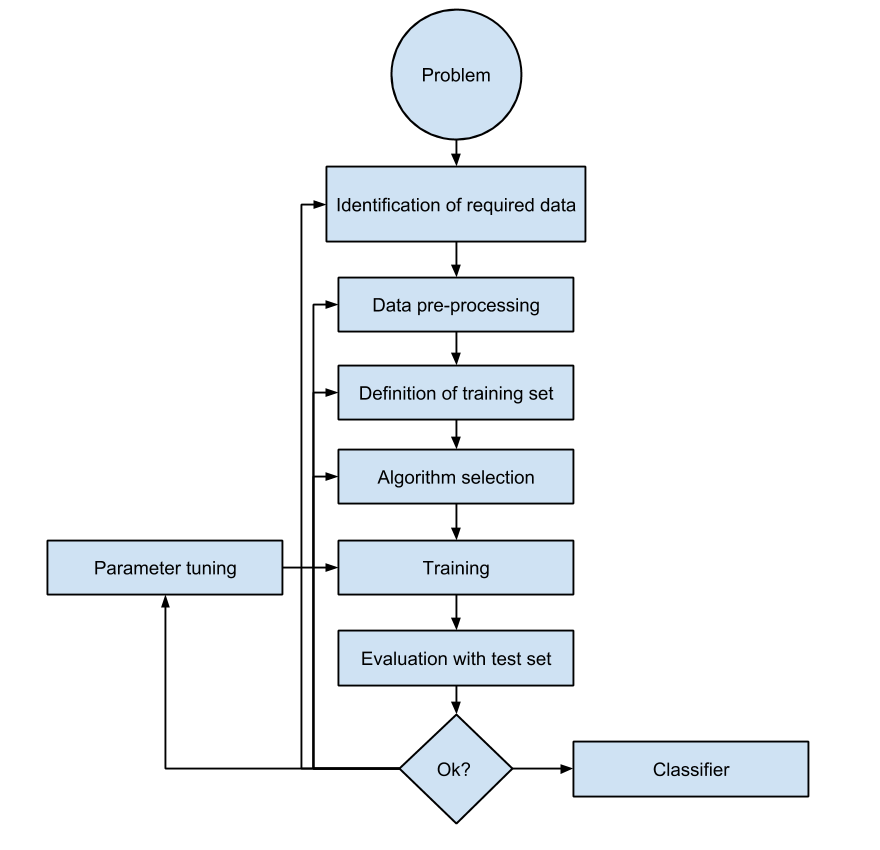
\includegraphics[width=0.8\linewidth]{images/ml_arch.png}
	\label{fig:arch_ml}
  \source{\cite{kotsiantis2007supervised}}
\end{figure}

\subsubsection{Árvore de Decisão}.
\subsubsection{Floresta Aleatória}
\subsubsection{K-ésimo Vizinho mais Próximo} 
\subsubsection{Máquina de Vetores de Suporte}
\subsubsection{Naive Bayes}
\subsubsection{Redes Neurais}
\subsubsection{Regressão Logística}

\todo[inline]{Escrever sobre cada algoritmo utilizado}


\subsection{Validação dos modelos de aprendizado supervisionado}
\label{modelValidation}

The validation of the models to classification tasks can be realized through metrics that has as inputs the number of real positive (P), negative (N) cases in the result of classification, true positive (TP), true negative (TN), false positive (FP) and false negative (FN) classifications. Following are some of the main metrics utilized to:

\begin{equation}
Accuracy = \frac{TP + TN}{P + N} = \frac{TP + TN}{TP + TN + FP + FN}
\end{equation}

\begin{equation}
Precision = \frac{TP}{TP + FP}
\end{equation}

\begin{equation}
Recall = \frac{TP}{P} = \frac{TP}{TP + FN}
\end{equation}

\begin{equation}
F_1 score = \frac{Precision * Recall}{Precision + Recall} = \frac{2TP}{2TP + FP + FN}
\end{equation}

\section{Term frequency–Inverse document frequency}

TF-IDF é um algoritmo de ponderação de variáveis que combina as ponderações \emph{frequência do termo} \nomenclature{TF}{\textit{Term Frequency}}{(TF --- \textit{Term Frequency})} e \emph{inverso da frequência nos documentos} (\nomenclature{IDF}{nverse Document Frequency}{IDF --- \textit{Inverse Document Frequency}}) para calcular os pesos dos termos linguísticos (variáveis) em um determinado corpus. Em outras palavras, o peso da variável é proporcional a frequência com a qual aparece nos documentos, e inversamente proporcional a quantidade de documentos que contém o termo linguístico em questão \cite{wu2018improved, yahav2018comments}. 


Dentre as variações de implementação da ponderação $W_{t,d}$ (TF-IDF) existentes, a abordagem tradicional considera uma coleção de termos $t \in T$ que aparecem em um conjunto de N documentos $d \in D$, posto isso, defini-se como o produto entre $tf_{i,j}$ e $idf_i$ --- onde $n_{i,j}$ é a frequência do termo $t_i$ no documento $d_j$, $\sum_k n_{k,j}$ o somatório da frequência de todos os termos do documento $d_j$ e $n$ o número de documentos onde $t_i$ aparece ($n + 1$, caso $n = 0$) --- conforme a seguinte equação \cite{wu2018improved}:

\begin{equation}
\begin{split}
tf_{i,j} = \frac{n_{i,j}}{\sum_k n_{k,j}}
\\
idf_i = \log \frac{N}{n + 1}
\\
W_{t,d} = tf_{t,d} * idf_t
\end{split}
\end{equation}

No contexto deste trabalho, entendemos documentos como as classes dos eventos de exceção. A \emph{frequência dos termos} (TF --- $tf_{t,d}$) é determinada por classe e a \emph{frequência do termo - inverso da frequência nos documentos} (IDF --- $idf_t $) como o inverso dos eventos de exceção, sendo $N$ o tamanho do conjunto dos eventos de exceção, sob o qual $df_t$ é definido. Os eventos de exceção são classificados em suas respectivas classes por meio dos modelos de aprendizado supervisionado, elencados na subseção \ref{supervisionedLearning}. 


\chapter{Revisão Sistemática}
\label{revisao}
Este capítulo apresenta uma Revisão Sistemática (RS) com o objetivo de encontrar o estado da arte de trabalhos que visam melhorar sistemas de transporte público por meio do processamento de \textit{tweets}. Além disso, de uma forma mais ampla, busca-se também entender como os \textit{tweets} têm sido utilizados na caracterização de problemas urbanos. Sendo assim, o capítulo é iniciado com a seção sobre o planejamento da Revisão Sistemática; seguida das questões de pesquisa utilizadas na formulação do problema da RS; do processo de coleta dos estudos primários; da avaliação dos dados coletados; da análise e interpretação dos estudos selecionados, concluindo com as considerações finais.

% \begin{CCSXML}
% <ccs2012>
% <concept>
% <concept_id>10003120.10003130.10003134.10003293</concept_id>
% <concept_desc>Human-centered computing~Social network analysis</concept_desc>
% <concept_significance>500</concept_significance>
% </concept>
% <concept>
% <concept_id>10011007.10011074.10011081.10011082.10011083</concept_id>
% <concept_desc>Software and its engineering~Agile software development</concept_desc>
% <concept_significance>500</concept_significance>
% </concept>
% </ccs2012>
% \end{CCSXML}

% \ccsdesc[500]{Human-centered computing~Social network analysis}
% \ccsdesc[500]{Software and its engineering~Agile software development}

\section{Planejamento da Revisão Sistemática}
\label{planejamento}
A presente Revisão Sistemática utiliza a metodologia proposta por \citeauthor{biolchini2005techincal} (\citeyear{biolchini2005techincal}), composta por cinco etapas.
A primeira etapa está relacionada à formulação do problema, na qual é levantada uma questão central se referindo ao tipo de evidência que deverá  estar contida na revisão. Em seguida, são construídas definições que permitem estabelecer uma distinção entre os estudos relevantes e irrelevantes para o propósito específico do que se está investigando \cite{biolchini2005techincal}.

A segunda etapa da condução está relacionada à Coleta de Dados, na qual são definidos os procedimentos que serão utilizados para encontrar a evidência relevante que foi definida na etapa anterior. Nesta fase é extremamente importante determinar as fontes que podem fornecer estudos relevantes a serem incluídos na pesquisa \cite{biolchini2005techincal}.

Na terceira etapa a Avaliação de Dados é definida, na qual são selecionadas as fontes primárias que deverão ser incluídas na revisão. Em seguida,  são aplicados os critérios de qualidade para separar estudos que podem ser considerados válidos, e determinadas as diretrizes para o tipo de informação que deve ser extraída dos relatórios de pesquisas primárias \cite{biolchini2005techincal}.

A quarta etapa da revisão é o processo de Análise e Interpretação, na qual os dados dos estudos primários válidos são sintetizados. E, na quinta etapa são realizados os processos de Conclusão e Apresentação \cite{biolchini2005techincal}.

\subsection{Justificativa da Revisão Sistemática}
\label{justificativa}
Esta Revisão Sistemática se justifica por não terem sido encontradas revisões sistemáticas com o foco em questões urbanas e de transporte público, abordando unicamente o processamento de \textit{tweets}. Em \cite{Chaniotakis2016}, por exemplo, foi realizado um mapeamento de forma não sistemática dos trabalhos sobre o uso das mídias sociais em problemas relacionados ao transporte público; \cite{steiger2015advanced}, por outro lado, desenvolveram uma revisão sistemática sobre o uso do Twitter para questões espaço-temporais; e \cite{jungherr2016twitter} no contexto político.%

Devido a isso, a presente revisão sistemática se diferencia por ter como objetivo encontrar o estado da arte de trabalhos que visam melhorar sistemas de transporte público por meio do processamento de \textit{tweets}. Além disso, de uma forma mais ampla, busca-se também entender como os \textit{tweets} têm sido utilizados na caracterização  de problemas urbanos.

\section{Questões de Pesquisa}
\label{questoes}
Nesta seção, são apresentadas as questões de pesquisa utilizadas para a formulação dos problemas abordados por essa Revisão Sistemática. Por meio das quais, busca-se atender os objetivos já mencionados na seção \ref{justificativa}.

\begin{enumerate}

\item Quais os tipos de problemas urbanos abordados utilizando processamentos de \textit{tweets}?
\label{item:1} \newline \newline
O propósito da \nomenclature{QP}{Questão de Pesquisa}{QP1} é identificar quais são as contribuições do processamento de \textit{tweets} para a mitigação de problemas urbanos. A resposta a essa questão de pesquisa ajudará especialistas das áreas multidisciplinares relacionadas ao Urbanismo (como a de Análise de Redes Sociais e Políticas Públicas) a terem um panorama de como \textit{tweets} podem ser utilizados para ajudar na solução de problemas urbanos. \newline

Uma análise preliminar dos estudos primários permite elaborar a seguinte \nomenclature{HP}{Hipótese de Pesquisa}{Hipótese de Pesquisa (HP1):} alguns dos problemas urbanos abordados estão relacionados ao transporte, mobilidade urbana, turismo e desastres naturais. \newline

\item Como \textit{tweets} têm sido utilizados para abordar problemas relacionados ao transporte público? \newline \newline
\label{item:2}
O propósito da QP2 é identificar se \textit{tweets} têm sido utilizados para solucionar problemas relacionados ao transporte público. A resposta a essa questão de pesquisa ajudará especialistas das áreas multidisciplinares relacionadas ao Urbanismo (como a de Análise de Redes Sociais e Políticas Públicas) a terem um panorama de como \textit{tweets} podem ser utilizados para ajudar na solução de problemas referentes a mobilidade urbana. \newline

Uma análise preliminar dos estudos primários permite elaborar a seguinte Hipótese de Pesquisa (HP2): \textit{tweets} têm sido utilizados principalmente para questões relacionadas ao congestionamento, não tendo como foco o transporte público.\newline

\item Quais as técnicas estatísticas utilizadas no processamento de \textit{tweets}?
\label{item:3} \newline \newline
O propósito da QP3 é identificar quais as técnicas estatísticas utilizadas no processamento de \textit{tweets}, principalmente no que se refere a análise de acurácia de classificação binária. A resposta a essa questão de pesquisa ajudará especialistas a terem um panorama de como garantir a confiabilidade ao utilizar dados oriundos de \textit{tweets}, dentre outros aspectos relacionados a testes estatísticos. \newline

Uma análise preliminar dos estudos primários permite elaborar a seguinte Hipótese de Pesquisa (HP3): \textit{${F_1}$ score} é a principal técnica estatística utilizada para análise de acurácia de classificação binária.\newline

\item Quais os paradigmas de processamento têm sido utilizados ao lidar com \textit{tweets}?
\label{item:4} \newline \newline
O propósito da QP4 é identificar os paradigmas utilizados para processamento de \textit{tweets}. A resposta a essa questão de pesquisa ajudará especialistas a terem um panorama das técnicas de processamento utilizadas na análise de \textit{tweets}. \newline

Uma análise preliminar dos estudos primários permite elaborar a seguinte Hipótese de Pesquisa (HP4): o principal paradigma utilizado tem sido o processamento de \textit{tweets} em \textit{batch} (\textit{offline}), após um processo de armazenamento. Poucos são os estudos que constroem uma plataforma para processamento de dados em tempo real. \newline

\item Quais são os eventos de exceção relacionados ao transporte público?
\label{item:5} \newline \newline
O propósito da QP5 é identificar os eventos de exceção relacionados ao transporte público. A resposta a essa questão de pesquisa ajudará especialistas no levantamento de eventos de exceção relacionados ao transporte público, os quais podem ser utilizados em algoritmos de classificação.\newline

Uma análise preliminar dos estudos primários permite elaborar a seguinte Hipótese de Pesquisa (HP5): há poucos ou nenhum estudo que, ao tratar de problemáticas relacionadas ao transporte público, realizam um levantamento dos eventos de exceção desse contexto.\newline

\item Quais as técnicas de Aprendizado de Máquina utilizadas no processamento de \textit{tweets}?
\label{item:6} \newline \newline
O propósito da QP6 é identificar as técnicas de Aprendizado de Máquina utilizadas no processamento de \textit{tweets}. A resposta a essa questão de pesquisa ajudará especialistas a terem um panorama das principais técnicas de Aprendizado de Máquina utilizadas no processamento de \textit{tweets}. \newline

Uma análise preliminar dos estudos primários permite elaborar a seguinte Hipótese de Pesquisa (HP6): a técnica \textit{Support Vector Machine} tem sido utilizada na maioria dos estudos que aplicam aos \textit{tweets} algum algoritmo de Aprendizado de Máquina.\newline
\end{enumerate}

\section{Coleta de dados}
\label{coleta}
Nesta Revisão Sistemática, os artigos foram coletados em quatro fontes de pesquisa, por meio da plataforma de indexação de trabalhos acadêmicos \textit{Google Scholar}\footnote{\url{https://scholar.google.com}. Acesso em Outubro, 29 de 2017.}. Constam na tabela \ref{tab:tableNumberOfArticles} as bases pesquisadas no ano de 2017, quantidades de artigos coletados, descartados no processo de filtragem (Fig. \ref{fig:filter}, descrito na seção \ref{avaliacao}) e selecionados. Com base na QP1, a seguinte \textit{string} de busca foi construída; restrita aos trabalhos publicados entre 2011 e 2016, escritos no idioma Inglês (devido ao fato das publicações relevantes, na área de Computação, estarem disponíveis nesse idioma): \newline 

\textbf{\textit{String} de busca:} twitter urban planning city (analytics OR patterns OR tweets OR social OR media) AND (public transport) \newline

\textbf{Palavras-chave:} twitter, urban, planning, city, analytics, patterns, tweets, social, media e public transport.

\begin{table}[!htb]
\centering
\caption{Quantidades de artigos coletados e fontes de busca}
	\label{tab:tableNumberOfArticles}
\begin{tabular}{c|c|c|c}
\hline
\textbf{Fonte} & \textbf {Artigos coletados} & \textbf{Filtragem} & \textbf{Selecionados}\\ 
\hline
\nomenclature{ACM}{\textit{Association for Computing Machinery}}{ACM} & 44 & 34 & 10 \\ 
\hline
\nomenclature{IEEE}{\textit{Institute of Electrical and Electronics Engineers}}{IEEE} & 82 & 74 & 8 \\ 
\hline
Elsevier & 81 & 72 & 9\\ 
\hline
Springer & 22 & 20 & 2\\ 
\hline
{-} & 229 & 200 & 29\\ 
\hline
\end{tabular}
\center{\textbf{Fonte:}} Felipe Cordeiro Alves Dias
\end{table}

\begin{figure}[H]% H manda colocar exatamente nessa posição no texto (relativa aos parágrafos anterior e posterior)
	\centering
 	  \caption{Processo de Filtragem}
		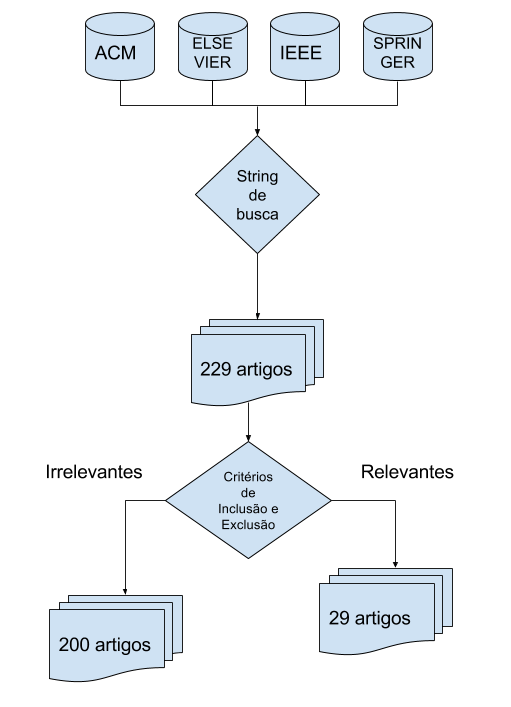
\includegraphics[width=0.5\linewidth]{images/metodologia_metodologia.png}
	\label{fig:filter}
  \source{Felipe Cordeiro Alves Dias, 2017}
\end{figure}

\section{Avaliação de Dados}
\label{avaliacao}

Visando selecionar os artigos relevantes para esta Revisão Sistemática, os seguintes critérios foram utilizados no processo de filtragem:

\begin{itemize}
\item Trabalho publicado (critério de qualidade).
\item Trabalhos que utilizam \textit{tweets} para abordar questões urbanas e de transporte público.
\item Trabalhos duplicados.
\item Trabalhos que estão fora do escopo da questão de pesquisa.
\end{itemize}

O processo de condução da Revisão Sistemática foi realizado utilizando os critérios acima mencionados, e está disponível em \citeauthor{fcas} (\citeyear{fcas}) (não incluso neste trabalho com o objetivo de não deixar o texto exaustivo), assim como seu respectivo protocolo (no qual contém o detalhamento dos critérios de inclusão e exclusão, dentre outros artefatos da condução). Após o processo de condução, alguns dos metadados dos artigos selecionados foram sintetizados.

Sendo assim, a Fig. \ref{fig:w_cloud} apresenta uma nuvem de \textit{tags} (gerada com a biblioteca \textit{wordcloud} \cite{wordcloud}) sintetizando as palavras chaves dos estudos primários selecionados; e a Fig. \ref{fig:qtd} a quantidade de artigos publicados por ano, sendo possível analisar por meio dela a distribuição dos artigos entre 2011 e 2016, assim como sua respectiva porcentagem, ilustrada na Fig. \ref{fig:porcentagem}.

\begin{figure}[H]% H manda colocar exatamente nessa posição no texto (relativa aos parágrafos anterior e posterior)
	\centering
 	  \caption{Quantidade de artigos publicados por ano}
		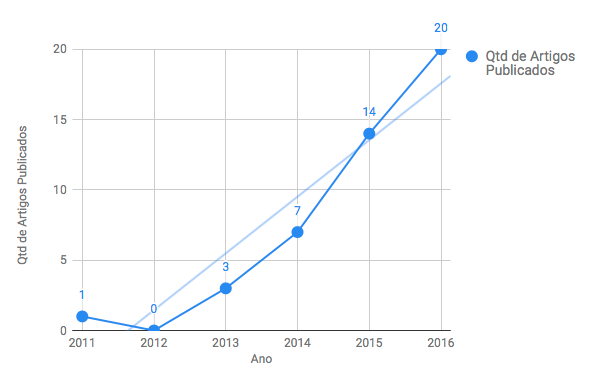
\includegraphics[width=0.8\linewidth]{images/g1.png}
	\label{fig:qtd}
  \source{Felipe Cordeiro Alves Dias, 2017}
\end{figure}

\begin{figure}[H]% H manda colocar exatamente nessa posição no texto (relativa aos parágrafos anterior e posterior)
	\centering
 	  \caption{Porcentagem dos artigos publicados por ano}
		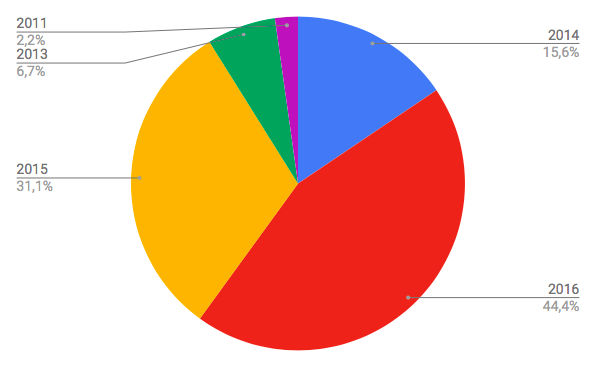
\includegraphics[width=0.8\linewidth]{images/g2.png}
	\label{fig:porcentagem}
  \source{Felipe Cordeiro Alves Dias, 2017}
\end{figure}

\begin{figure}[H]% H manda colocar exatamente nessa posição no texto (relativa aos parágrafos anterior e posterior)
	\centering
 	  \caption{Nuvem de palavras das \textit{keywords} dos artigos selecionados}
		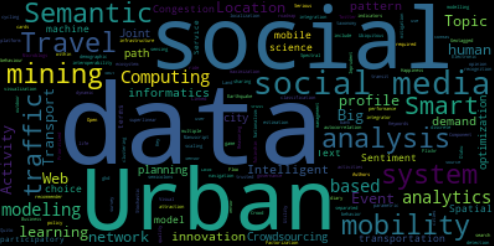
\includegraphics[width=0.8\linewidth]{images/world_cloud_metodologia.png}
	\label{fig:w_cloud}
  \source{Felipe Cordeiro Alves Dias, 2017}
\end{figure}

\section{Análise e Interpretação}
\label{analise}
Nesta seção é realizada a análise e interpretação dos estudos primários selecionados pela Revisão Sistemática, sendo as subseções divididas de acordo com as questões de pesquisa.
\subsection{Tipos de problemas urbanos abordados utilizando o processamento \textit{tweets} (QP1)}

Os tipos de problemas urbanos abordados utilizando o processamento de \textit{tweets} foram divididos nas seguintes categorias: 

\begin{enumerate}
\item \textit{\textbf{e-Participation}} (Interação entre  cidadãos  e órgãos civis) \cite{Mukherjee2015}, \cite{Soomro2016}.
\item \textbf{Detecção de zoneamento urbano} \cite{Frias-Martinez2014}.
\item \textbf{Identificação de pontos de interesse} \cite{Farseev2015}, \cite{Gutev2016}, \cite{Bendler2014}, \cite{Abbasi2015}, \cite{Gkiotsalitis2015}, \cite{Gkiotsalitis2016}, \cite{Hasan2014}, \cite{Maghrebi2015}, \cite{DiLorenzo2013}.
\item \textbf{Mobilidade} \cite{Gutev2016}, \cite{Chen2016}, \cite{Yousaf2014}.
\item \textbf{Padrões demográficos} \cite{Farseev2015}, \cite{Gutev2016}, \cite{Steiger2015Census}, \cite{Guo2016}.
\item \textbf{Poluição} \cite{Zagal2016}.
\item \textbf{Segurança Pública} \cite{Wen2016}, \cite{Mata2015}.
\item \textbf{Turismo} \cite{Thomaz2016}, \cite{Abbasi2015}, \cite{Chua2016}, \cite{Sobolevsky2015}.
\item \textbf{Tráfego} \cite{Anantharam2015}, \cite{Lecue2014}.
\end{enumerate}

Conforme os estudos primários analisados pela Revisão Sistemática, e enumerados nessa seção, é possível interpretar que \textit{tweets} podem ser utilizados para auxiliar na mitigação de inúmeros problemas urbanos. Apesar disso, \cite{Chaniotakis2015} observam que os \textit{tweets} contendo informações sobre geolocalização são normalmente publicados em áreas relacionadas ao lazer, além de haver correlação entre regiões urbanas com maior renda \textit{per capita} e o número de \textit{tweets} postados. Tal evidência pode conduzir viés nas análises por representar somente algumas classes econômicas da população. 

Considerando a observação anterior, um dos estudos analisados foi o realizado por \cite{Zagal2016}, na Cidade do México. Nesse estudo, foram mapeados os pontos da cidade referenciados em publicações relacionadas a doenças respiratórias e poluição, orientando tomadas de decisão no aspecto ambiental. 

Além disso, há também exemplos de trabalhos relacionados a Segurança Pública, como o estudo de caso realizado por \cite{Wen2016}, no qual foi enriquecido um conjunto de dados com \textit{tweets} geolocalizados, visando analisar o impacto dos ataques terroristas (em Paris, em novembro de 2015) nos padrões de atividades urbanas (relacionadas ao uso de transporte público, serviços, realização de compras, e atividade noturna). Em um outro caso de aplicação, estimou-se por meio de \textit{tweets}, a probabilidade de ocorrência de crimes e ameaças nas ruas da Cidade do México, sugerindo rotas seguras aos pedestres \cite{Mata2015}.

Também, foram encontrados na literatura estudos que utilizaram \textit{tweets} para inferir padrões demográficos. Por exemplo, em \cite{Farseev2015}; \cite{Gkiotsalitis2015}; \cite{Gkiotsalitis2016}, \textit{tweets} foram processados para analisar a distribuição etária e de gênero da população, assim como seus respectivos pontos de interesse \cite{Hasan2014} e \cite{Maghrebi2015} (como locais para entretenimento, residência, trabalho, recriação, compras, educação e serviços sociais). 

Tais pontos de interesse, podem ser utilizados em problemas relacionados ao transporte público \cite{Gutev2016} e também ao Turismo, como no estudo realizado por \cite{Abbasi2015} para identificar a locomoção de visitantes e residentes em pontos turísticos de Sydney; por \cite{Chua2016}, ao caracterizar aspectos espaciais, temporais e demográficos, dos turistas da cidade de Cilento, Itália; e por \cite{Thomaz2016} na cidade de Curitiba (Brasil), no contexto da Copa do Mundo de 2014.

Nesse mesmo contexto, \cite{Guo2016} estudaram algumas questões demográficas via análise de sentimento, encontrando correlação positiva entre oportunidades de emprego e sentimentos positivos, e negativa entre felicidade e número de crianças na população da Grande Londres. Outro caso de uso, foi o desenvolvido em \cite{Steiger2015Census}, no qual \textit{tweets} foram processados para identificar diferentes tipos de atividades em Londres, correlacionando-as com informações censitárias; e em \cite{Sobolevsky2015} ao estudar a atratividade da Espanha a turistas.

Um dos problemas relacionados à identificação de pontos de interesse se refere as incertezas espaço-temporais e de determinação de tópicos, o qual foi abordado pelo trabalho realizado por \cite{Bendler2014}. Nele, os autores contribuíram com uma técnica para minimizar o problema ao processar \textit{tweets}; analisando a causalidade entre o tempo e local das postagens realizadas, reduzindo assim os índices de incerteza, no contexto da cidade de São Francisco, EUA. Outro problema, relaciona-se com a questão da privacidade, pois as localizações dos usuários podem ser inferidas mesmo quando não disponibilizadas. Nesse cenário, \cite{Wang2017} propõem um \nomenclature{PTCS}{Sistema de Calibração de Trajetórias Privadas}{Sistema de Calibração de Trajetórias Privadas (PTCS),} usando os mecanismos de Privacidade Diferencial e de \textit{k-anonymity}, com isso é possível extrair informações sobre trajetórias sem exposição de informações sensíveis, testado na extração de localizações por meio de \textit{tweets}. 

Outro contexto na literatura revisada está relacionado ao processamento dos eventos que acontecem na cidade (idealmente em tempo real, como sugerem \cite{Soomro2016}). Um dos estudos encontrados sobre esse assunto, foi o realizado por \cite{Anantharam2015}, no qual foi desenvolvida uma técnica para identificar os diferentes tipos de eventos do cotidiano urbano, rotulando-os sequencialmente, por meio da anotação de \textit{tweets} e extração de eventos, considerando aspectos espaciais, temporais e temáticos. Para isso, utilizou conhecimentos de domínio, tais como informações sobre os locais em uma cidade e possíveis termos para os eventos, identificando assim os relacionados ao tráfego da região da Baia de São Francisco, EUA. 

Sobre a mesma temática, \cite{DiLorenzo2013} desenvolveram uma ferramenta inteligente e interativa para exploração visual da dinâmica de eventos sociais ao longo das dimensões espacial, temporal e organizacional. O tráfego também foi objeto de estudo em \cite{Chen2016}, ao relacionar eventos do trânsito com a demanda por bicicletas; e em \cite{Lecue2014}, ao demonstrar uma plataforma para análise inteligente do tráfego (em tempo real), com base em fontes heterogêneas de dados (incluindo \textit{tweets} de agências oficiais de trânsito).

Em uma abordagem mais genérica, \cite{Mukherjee2015} propuseram uma plataforma para processar (em \textit{near real time}) questões urgentes da cidade, oriundas de diversas fontes (incluindo o \textit{Twitter}), atuando como intermediadora entre cidadãos e agências civis. No que se refere a mobilidade urbana, mas não utilizando informações sobre pontos de interesse, \cite{Yousaf2014} inferiram a afinidade entre usuários por meio da análise de \textit{retweets}, possibilitando que rotas de corridas sejam compartilhadas entre pessoas com interesses em comum, tornando a viagem mais agradável.

De forma inusitada, \cite{Frias-Martinez2014} utilizaram apenas \textit{tweets} geolocalizados para analisar suas respectivas distribuições no espaço urbano, visando identificar a caracterização do uso da terra, considerando os zoneamentos urbanos industriais, residenciais, comerciais e de lazer. O trabalho foi realizado no contexto da cidade de Manhattan (EUA), Londres (Reino Unido) e Madrid (Espanha).

\subsection{Casos de uso relacionados ao transporte público (QP2)}
Nesta seção, são identificados os estudos primários que utilizam processamento de \textit{tweets} tendo como foco a mitigação dos problemas relacionados ao transporte público; enumerados a seguir:
\begin{enumerate}
\item \textbf{Impacto de eventos no transporte público}.
\begin{enumerate}
\item Impacto dos ataques terroristas em Paris no uso do transporte público \cite{Wen2016}.
\item Impacto de eventos relacionados ao tráfego na demanda por bicicletas, em Nova Iorque e Washington D.C, EUA \cite{Chen2016}.
\item Impacto dos pontos de interesse na demanda por transporte público \cite{Maghrebi2015}.
\item Impacto dos eventos anormais nas tomadas de decisão dos passageiros do Metrô de Tokyo \cite{Itoh2016}.
\item Predição de fluxo de passageiros no Metrô de Nova Iorque \cite{Ni2016}.
\end{enumerate}

\item \textbf{Planejamento e gestão do transporte público}.
\begin{enumerate}
\item Análise de sentimento relacionada ao acesso ao transporte público \cite{Guo2016}.
\item Coleta de informações relacionadas ao transporte público \cite{Gal-Tzur2014}.
\item Identificação de locais para estações de bicicletas, em St. Petersburg, Rússia \cite{Gutev2016}.
\item Identificação da disposição dos usuários para realizar viagens de lazer \cite{Gkiotsalitis2016}.
\item Plataforma para notificação de problemas relacionados ao transporte público de Bangalore, Índia \cite{Mukherjee2015}.
\end{enumerate} 
\end{enumerate}

Conforme os estudos primários analisados pela Revisão Sistemática, e enumerados nessa seção, é possível interpretar que os estudos estão classificados em análise de impacto de eventos, planejamento e gestão do transporte público. Por exemplo, \cite{Wen2016} utilizaram \textit{tweets} para analisar o impacto dos ataques terroristas em Paris (2015) nos padrões de mobilidade referentes ao uso de transporte público. Semelhantemente, \citeauthor{Itoh2016} (\citeyear{Itoh2016}) desenvolveram uma ferramenta para analisar e explorar visualmente, com base em \textit{tweets}, as tomadas de decisão dos passageiros do Metrô de Tokyo, ante a eventos anormais, tais como Tufões, Incêndios, Terremotos, dentre outros. Nesse mesmo contexto, \cite{Ni2016} propuseram uma técnica de predição de fluxo de passageiros no Metrô de Nova Iorque, identificando eventos com base nas \textit{hashtags} dos \textit{tweets}. Enquanto que em \cite{Chen2016}, analisaram a relação entre eventos do tráfego com a demanda por bicicletas.

No que se refere aos estudos focados no planejamento e gestão do transporte público, \cite{Mukherjee2015} apresentam uma plataforma desenvolvida e utilizada pela Agência de Transporte Público de Bangalore, na Índia, a qual permite que usuários reportem questões relacionadas ao transporte  público, possibilitando a melhoria do planejamento de suas respectivas operações, assim como o serviço prestado para a população. Nessa mesma linha de estudo, em \cite{Gutev2016}, \textit{tweets} são utilizados para identificar a popularidade de determinados locais, pontos de interesse e distribuição etária, com o objetivo de determinar os melhores pontos para estações de bicicletas e incentivar assim o uso desse modal de transporte. Também relacionado aos pontos de interesse, \cite{Maghrebi2015} utilizaram \textit{tweets} para identificar padrões das atividades humanas (em diferentes horários do dia) e seus respectivos impactos na demanda por transporte público.

Em \cite{Gal-Tzur2014}, por sua vez, utilizaram uma abordagem hierárquica para classificar \textit{tweets} relacionados ao transporte. Com isso, demonstraram que é possível usar essas informações para fins de planejamento e gerenciamento do transporte. Tal técnica, foi aplicada em um estudo de caso associado a eventos esportivos, ocorridos no Reino Unido. A hierarquia é composta por três níveis, no primeiro, os \textit{tweets} são classificados entre os que expressam a necessidade de serviços de transporte, opiniões e incidentes; o segundo, identifica a categoria do transporte; e último, relaciona \textit{tweets} a tópicos. 

Outro estudo que contribui com o planejamento do transporte público, é o realizado em (\citeauthor{Gkiotsalitis2015}, \citeyear{Gkiotsalitis2015}, \citeyear{Gkiotsalitis2016}), no qual \textit{tweets} foram processados para identificar a disposição dos usuários para realizar viagens relacionadas ao lazer (pontos de interesse), sugerindo a eles atividades com menor tempo de percurso e probabilidade de atrasos. Além do tempo de percurso, outro ponto relevante considerado foi o de bom nível de acesso ao transporte público, o qual quando existente impacta positivamente na felicidade das pessoas e se correlaciona com sentimentos positivos, segundo a análise de sentimentos realizada por \cite{Guo2016}, utilizando \textit{tweets} publicados na Grande Londres.

\subsection{Técnicas estatísticas utilizadas no processamento de \textit{tweets} (QP3)}
Nesta seção, são apresentadas as técnicas estatísticas utilizadas pelos estudos primários, no processamento de \textit{tweets}, enumeradas a seguir:

\begin{enumerate}
\item \textbf{Análise de métricas relacionadas a desempenho} (erro de reconstrução relativo, qualidade dos componentes descritivos recuperados e qualidade dos componentes comuns recuperados) \cite{Wen2016}.
\item \textit{\textbf{Cosine similarity}} \cite{Yousaf2014}, \cite{Frias-Martinez2014}.
\item \textbf{\textit{\bm{${F_1}$} score}} \cite{Anantharam2015}, \cite{Chen2016}.
\item \textit{\textbf{Term frequency–inverse document frequency}} (TF-IDF) \cite{Mukherjee2015}.
\item \textit{\textbf{Inverse coefficient of variation}} \cite{Bendler2014}.
\item \textit{\textbf{Jackknife resampling}} \cite{Bendler2014}.
\item \nomenclature{LISA}{\textit{Local Indicators of Spatial Association}}{\textit{\textbf{Local Indicators of Spatial Association}} (LISA)} \cite{Steiger2015Census}.
\item \textit{\textbf{Local Moran's}} \cite{Steiger2015Census}.
\item \textit{\textbf{Maximum likelihood estimation}} \cite{Mukherjee2015}.
\item \nomenclature{SARIMA}{\textit{Seasonal Autoregressive Integrated Moving Average}}{\textit{\textbf{Seasonal Autoregressive Integrated Moving Average}} (SARIMA)} \cite{Ni2016}.
\item \textit{\textbf{Optimization and Prediction with hybrid loss function}} \cite{Ni2016}.
\end{enumerate}
 
Em \cite{Ni2016}, os autores utilizaram a técnica \textit{Seasonal Autoregressive Integrated Moving Average} em conjunto com Regressão Linear, propondo uma abordagem baseada em otimização paramétrica e convexa, chamada \textit{Optimization and Prediction with hybrid loss function}, adequada para modelagem utilizando séries temporais. Com isso, tal técnica foi aplicada na predição de fluxo de passageiros com base em \textit{hashtags} de \textit{tweets}.  

Referente aos problemas relacionados a ambiguidade e identificação de contextos, \cite{Anantharam2015}; \cite{Chen2016} e \cite{Gal-Tzur2014} aplicaram a técnica \textit{${F_1}$ score} para analisar a acurácia do processamento de \textit{tweets}. Por outro lado, em \cite{Mukherjee2015}, utilizaram a técnica \textit{Maximum likelihood estimation} para determinar a probabilidade de ocorrência de um evento, assim como a confiabilidade da informação.

No que se refere a agrupamento, \cite{Yousaf2014} agruparam usuários de acordo com a \textit{Cosine similarity}, unindo pessoas com interesses em comum nos mesmos grupos. \cite{Frias-Martinez2014}, por outro lado, usou a mesma técnica para agrupar \textit{tweets} de acordo com suas semelhanças quanto aos tipos de zoneamento urbano.

De forma isolada, no trabalho realizado por \cite{Mukherjee2015}, utilizaram a técnica TF-IDF na fase de classificação para o definir o \textit{score} de categorias de eventos, escolhendo a mais relevante a ser buscada em um dicionário de categorias. Também isoladamente, \cite{Steiger2015Census} usaram a técnica LISA na identificação de \textit{clusters} espaciais e valores esporádicos espaciais, obtendo assim os locais com atividades sociais. Além disso, também utilizaram a técnica \textit{Local Moran's} para detectar diferentes padrões de atividade de acordo com o espaço geográfico.

Por último, \cite{Bendler2014} inovaram ao utilizar a técnica \textit{Jackknife resampling} como inspiração para o desenvolvimento de uma abordagem que visa analisar a estabilidade estatística de um conjunto de categorias. Além disso, usaram também a análise \textit{Inverse Coefficient of variation} para verificar a dispersão negativa da distribuição de um conjunto de variáveis. 

\subsection{Paradigmas de processamento (QP4)}
Nesta seção, encontram-se a seguir apenas os paradigmas de processamento extraídos dos estudos primários analisados: 
\begin{enumerate}
\item \textit{\textbf{Batch processing}} (offline) \cite{Anantharam2015}, \cite{Wen2016}, \cite{Farseev2015}, \cite{Gutev2016}, \cite{Mata2015}, \cite{Chen2016}, \cite{Abbasi2015}, \cite{Bendler2014}, \cite{Bendler2014}, \cite{Yousaf2014}, \cite{Frias-Martinez2014}, \cite{Steiger2015Census}, \cite{Gal-Tzur2014}, \cite{Gkiotsalitis2016}, \cite{DiLorenzo2013}, \cite{Itoh2016}, \cite{Chaniotakis2015}.
\item \textit{\textbf{Near Real Time}} \cite{Mukherjee2015}.
\item \textit{\textbf{Real Time}} \cite{Soomro2016}, \cite{Lecue2014}.
\end{enumerate}

\subsection{Eventos de exceção relacionados ao transporte público (QP5)}
\label{qp5}

Nesta seção, encontram-se a seguir os eventos de exceção relacionados ao transporte público, extraídos dos estudos primários:

\begin{enumerate}
\item \textbf{Acidentes}.
\begin{enumerate}
\item Acidentes nas estações transporte \cite{Itoh2016}.
\item Incêndio \cite{Itoh2016}.
\end{enumerate}

\item \textbf{Espaço-temporais}.
\begin{enumerate}
\item Dia da semana \cite{Chen2016}.
\item Hora do dia \cite{Chen2016}.
\end{enumerate}

\item \textbf{Eventos sociais}.
\begin{enumerate}
\item Feiras de rua \cite{Chen2016}.
\item Festivais \cite{Chen2016}, \cite{Lecue2014}.
\item Jogos esportivos \cite{Chen2016}, \cite{Gal-Tzur2014}.
\item Passeatas e maratonas \cite{Chen2016}, \cite{Itoh2016}.
\end{enumerate}

\item \textbf{Eventos urbanos}.
\begin{enumerate}
\item Relacionados ao tráfego \cite{Chen2016}, \cite{Lecue2014}.
\end{enumerate}

\item \textbf{Desastres naturais}.
\begin{enumerate}
\item Tempestades \cite{Itoh2016}.
\item Terremoto \cite{Itoh2016}.
\item Tufões \cite{Itoh2016}.
\end{enumerate}

\item \textbf{Metereológicos}.
\begin{enumerate}
\item Dia claro, nublado, chuvoso, nevando, com neblina \cite{Chen2016}.
\item Temperatura do ar \cite{Chen2016}.
\end{enumerate}

\end{enumerate}

\subsection{Técnicas de Aprendizado de Máquina utilizadas no processamento de \textit{tweets} (QP6)}
\label{iaClassification}
Nesta seção, são apresentadas as técnicas de Aprendizado de Máquina utilizadas para processamento de \textit{tweets}, extraídas dos estudos primários e enumeradas a seguir:

\begin{enumerate}
\item \textit{\textbf{Bayes classification}} \cite{Mata2015}.
\item \textit{\textbf{C5.0 algorithm}} \cite{Zagal2016}.
\item \nomenclature{CRF}{\textit{Conditional Random Field}}{\textit{\textbf{Conditional Random Field (CRF) with Logistic Regression}}} \cite{Anantharam2015}.
%\item \textit{\textbf{Event extraction based on tweet hashtags}} \cite{Ni2016}.
\item \nomenclature{LDA}{\textit{Latent Dirichlet Allocation}}{\textbf{\textit{Latent Dirichlet Allocation} (LDA)}} \cite{Farseev2015}, \cite{Abbasi2015}, \cite{Hasan2014}, \cite{DiLorenzo2013}, \cite{Ni2016} .
\item \textit{\textbf{Linear Regression}} \cite{Gutev2016}, \cite{Bendler2014}, \cite{Ni2016}, \cite{Guo2016}.
\item \textit{\textbf{Monte Carlo simulation}} \cite{Chen2016}.
\item \textbf{\textit{PairFac}} (técnica inovadora que utiliza \textit{Tensor Factorization}) \cite{Wen2016}.
\item \textit{\textbf{Random Forest classification}} \cite{Farseev2015}.
\item \nomenclature{SVM}{\textit{Support Vector Machine}}{\textit{\textbf{Support Vector Machine}}} \cite{Mukherjee2015}, \cite{Gal-Tzur2014}.
\item \textit{\textbf{Self-Organizing Maps}} \cite{Frias-Martinez2014}.
\end{enumerate}

No contexto urbano, inúmeros eventos podem acontecer e impactar a população. O trabalho realizado por \cite{Wen2016}, desenvolveu uma técnica que utiliza a análise de tensores discriminantes para aprender e de forma automatizada descobrir os impactos de um determinado evento no cotidiano da cidade. Numa abordagem mais simples, \cite{Chen2016} utilizou \textit{Monte Carlo simulation} para treinar um modelo para predição de demanda por bicicletas, devido a dificuldade de encontrar exemplos suficientes para usar outras abordagens de treinamento. 

Especificamente sobre as técnicas de classificação, \cite{Mukherjee2015} utilizaram \textit{Support Vector Machine} para classificar os eventos recebidos de diversas fontes. Referente a essa abordagem, \cite{Gal-Tzur2014} analisaram inúmeras técnicas de Aprendizado de Máquina, obtendo a melhor performance com o SVM, além disso, observaram como principal vantagem a sua capacidade de adaptação ao gênero e tarefas subjacentes. 

Apesar disso, \cite{Guo2016} utilizaram Processamento de Linguagem Natural (baseado em palavras chaves) para rotular sentimentos de \textit{tweets}, devido a facilidade de escalar essa técnica (para processamento de milhões de \textit{tweets}), em comparação a SVM. Outro caso de divergência é o do estudo realizado por \cite{Farseev2015}, no qual foi escolhido o modelo de classificação \textit{Random Forest}, devido ao fato de ser mais adequado para classificação em espaço dimensional elevado, em vez das técnicas SVM e \textit{Naive Bayes}, no que se refere a predição de idade e gênero usando \textit{tweets}.

\citeauthor{Mata2015} (\citeyear{Mata2015}), por sua vez, aplicou a técnica \textit{Bayes Classification} em \textit{tweets}, visando obter probabilidades relacionadas a crimes e ameaças em uma determinada localização. Por outro lado, \cite{Zagal2016} usaram o \textit{C5.0 algorithm} devido ao melhor desempenho em relação a \textit{Bayes}, dependendo do tópico que está sendo classificado. 

Para anotação de eventos, \cite{Anantharam2015} treinaram um modelo CRF (usando anotações baseadas em dicionários) para determinar os locais da cidade e os termos relacionados aos eventos expressos em \textit{tweets}. E, isoladamente \cite{Frias-Martinez2014} utilizaram a técnica \textit{Self-Organizing Maps}, tendo como entrada os valores de latitude e longitude de \textit{tweets}. Com isso, construíram um mapa segmentado em áreas urbanas, baseando-se nas regiões com diferentes concentrações de \textit{tweets}.

Em relação a localidades, segundo \cite{Farseev2015}, a técnica LDA tem sido muito utilizada para identificação de pontos de interesses mencionados em \textit{tweets}, sendo adequada para grandes bases de dados e agrupamento de \textit{tweets} com tópicos similares, de acordo com \cite{Steiger2015Census}. \cite{Abbasi2015} exemplificou isso ao aplicar LDA para identificação de \textit{tweets} relacionados ao Turismo; \cite{Hasan2014}, para identificação de padrões de atividades humanas; e \cite{DiLorenzo2013}, para identificação de eventos sociais.

No entanto, \cite{Ni2016} em vez de usarem LDA, extraíram \textit{hashtags} de \textit{tweets} para um vetor, utilizando-o para medir as atividades sociais e identificar seus respectivos contextos. Segundo \cite{Ni2016}, isso se justifica devido ao fato de que há uma grande chance do alto volume de \textit{tweets} não indicar necessariamente eventos e atendimentos a eles. Além disso, afirmam que o método baseado em \textit{hashtag} é capaz de indicar sobre o que é o evento, mesmo não utilizando o Inglês formal.

Por sua vez, em \cite{Gutev2016}, os autores utilizaram \nomenclature{RL}{Regressão Linear}{Regressão Linear (RL)} para analisar a demanda por bicicletas de acordo com as localizações extraídas dos \textit{tweets}. Enquanto que \cite{Bendler2014} usaram RL para fornecer evidências de que as categorias dos pontos de interesse se relacionam com as variáveis referentes ao espectro espaço-temporal; e \cite{Guo2016} para analisar a correlação entre sentimentos positivos com as oportunidades de trabalho, com a quantidade de crianças, e com o acesso a transporte. 

\section{Considerações finais sobre a revisão sistemática}
\label{conclusao}
Em uma análise quantitativa dos estudos primários selecionados, podemos concluir que a quantidade de artigos publicados sobre o uso de \textit{tweets} na caracterização de problemas urbanos e relacionados ao transporte público tem crescido consideravelmente, entre 2011 e 2016. Provavelmente, devido ao fato da popularização das Redes Sociais e grande quantidade de dados disponíveis para processamento.

Tais estudos estão concentrados em maioria na identificação de pontos de interesse, utilizando-os em diferentes contextos, tais como o de turismo,mobilidade. Além disso, abordam também problemas relacionados ao transporte e desastres naturais, confirmando a primeira hipótese (HP1) dessa Revisão Sistemática. As temáticas não abordadas pela HP1 foram as relacionadas a \textit{e-Participation}, detecção de zoneamento urbano, padrões demográficos e segurança pública, demonstrando a variedade de problemas urbanos explorados com o processamento de \textit{tweets}.

Referente a segunda hipótese, os estudos exploraram principalmente o impacto de eventos no transporte público, confirmando-a parcialmente. Isso, devido ao fato de um dos trabalhos explorar como os eventos relacionados ao tráfego impactam na demanda por bicicletas; não havendo nenhum outro sobre processamento de \textit{tweets} para mitigação dos problemas envolvendo Tráfego. Outra temática não mencionada pela HP2 e sobre a qual há uma quantidade considerável de estudos, foi a do uso de \textit{tweets} para o planejamento e gerenciamento do transporte público.

Independentemente dos problemas abordados por meio do processamento de \textit{tweets}, dentre as 12 técnicas estatísticas elencadas, \textit{${F_1}$ score} foi a única referenciada como ferramenta para análise de acurácia de classificação binária, confirmando a terceira hipótese (HP3). Apesar disso, a HP3 não considerou outras técnicas importantes (com propósitos distintos), como a \textit{Linear Regression}, amplamente utilizada nos estudos analisados. Referente as técnicas de Aprendizado de Máquina, a mais utilizada foi a \textit{Latent Dirichlet Allocation} (LDA), seguida da \textit{Support Vector Machine} (SVM), confirmando parcialmente a sexta hipótese (HP6).

Por fim, apenas quatro dos vinte e nove estudos analisados, cerca de 14\%, mencionaram \textit{features} relacionadas ao transporte público, confirmando assim a quinta hipótese (HP5). Assim como a quantidade de trabalhos que realizam processamento de \textit{tweets} em tempo real, sendo apenas dois do total analisado, cerca de 6\%, que utilizam esse paradigma de processamento, o que confirma a quarta hipótese (HP4). É importante ainda observar que, outros estudos que mencionaram processamento em tempo real, realizaram na verdade coleta de \textit{tweets} em tempo real, para análises a posteriori via processamento em \textit{batch} (offline), categoria na qual a maioria dos estudos foram enquadrados.

\chapter{Construção do conjunto de dados}
\label{dataSet}

Nesta seção, são apresentados os conjuntos de dados referentes a proposta de pesquisa.

\subsection{\textit{Corpus Twitter}}

A Rede Social \textit{Twitter}, foi escolhida como fonte de dados para a construção do conjunto de dados relacionados aos eventos de exceção. Isso devido ao fato de cada publicação ser limitada em 280 caracteres, o que reduz a complexidade de processamento do conteúdo publicado, e devido aos estudos existentes abordando problemas urbanos e de mobilidade urbana, conforme os analisados na revisão sistemática do Cap. \ref{revisao}.

Assim, o conjunto de dados utilizado para a identificação dos eventos de exceção é composto por \textit{tweets}, em português brasileiro, dos \textit{profiles} contidos na tabela \ref{tab:oficialProfiles}. É importante observar que, para esse projeto de pesquisa, apenas os \textit{tweets} publicados pelas contas selecionadas serão considerados, descartando os relacionados às interações entre diferentes \textit{profiles} (\textit{retweets} e \textit{replies}). Ou seja, os dados utilizados estão relacionados ao canal unidirecional de comunicação (no contexto de \textit{e-participation}). Com essa restrição, evitamos problemas referentes a confiabilidade dos dados, o que nos permite focarmos na caracterização dos eventos de exceção e de seus respectivos impactos.

Sobre a seleção dos \textit{profiles}, todos foram selecionados manualmente de acordo com os órgãos responsáveis por notificar eventos de exceção. Tais \textit{profiles} são de caráter público, ou seja, o acesso aos \textit{tweets} não envolve questões de privacidade.
Apesar do acesso facilitado aos \textit{tweets}, a API do \textit{Twitter} limita a quantidade e frequência de requisições aos \textit{endpoints}. Por exemplo, no protótipo desenvolvido (na linguagem de programação Java), há um artefato que coleta (utilizando o \textit{plugin} \textit{Twitter4J}\footnote{\url{twitter4j.org}. Acesso em Outubro, 29 de 2017.}) os 3.200 \textit{tweets} mais recentes (se disponíveis) de cada conta, através do \textit{endpoint} \textit{statuses/user\_timeline}; o qual permite no máximo 180 requisições, em um intervalo de 15 minutos, com autenticação via conta de usuário\footnote{\url{https://dev.twitter.com}. Acesso em Outubro, 29 de 2017.}.

Durante a coleta dos \textit{tweets}, eles são mapeados para a seguinte classe do modelo da aplicação: \textit{TweetInfo}, que contém as informações respectivas ao \textit{id}, texto da publicação, \textit{timestamp}, endereço extraído, latitude e longitude. Em seguida, o modelo é persistido no banco de dados não relacional \textit{MongoDB}\footnote{\url{https://www.mongodb.com}. Acesso em Outubro, 29 de 2017.} e também no banco de dados de séries temporais \textit{Druid}\footnote{\url{http://druid.io}. Acesso em Outubro, 29 de 2017.} para exploração e visualização dos dados, processo explicado na seção \ref{dataViz}. Os detalhes sobre o intervalo de tempo e o número de \textit{tweets} coletados constam na tabela \ref{tab:tweetsCollected}.

\begin{table}[!htb]
\centering
\caption{Intervalo de tempo e número de \textit{tweets} coletados}
	\label{tab:tweetsCollected}
\begin{threeparttable}
\begin{tabular}{c|c|c|c}
\hline
\textbf {Profile no \textit{Twitter}} &\textbf{ \# tweets \tnote{a}}  &\textbf{ \textit{Timestamp 1 \tnote{b}}} & \textbf{\textit{Timestamp 2 \tnote{c}}} \\ 
\hline
BombeirosPMESP & 5.750 & 2017-05-21 02:10:39 & 2017-10-29 23:07:08  \\
\hline
CETSP\_ & 5.042 & 2017-02-20 14:07:04 & 2017-10-29 21:45:54 \\ 
\hline
CPTM\_oficial & 5.435 & 2017-04-24 13:00:17 & 2017-10-29 10:00:40 \\ 
\hline
governosp & 5.450 & 2017-05-10 17:00:05 & 2017-10-29 22:00:03 \\
\hline
metrosp\_oficial & 7.296 & 2017-06-07 17:23:34  & 2017-10-29 17:48:12 \\
\hline
Policia\_Civil & 3.360 & 2015-04-15 17:44:44 & 2017-10-27 10:01:53 \\  
\hline
PMESP & 3.956 & 2016-06-02 17:21:32 & 2017-10-29 20:25:37 \\ 
\hline
saopaulo\_agora & 3.671 & 2016-11-18 07:36:12 & 2017-10-29 20:56:28 \\
\hline
smtsp\_ & 1.128 & 2017-04-26 10:44:26 & 2017-10-29 23:00:11 \\ 
\hline
SPCEDEC & 945 & 2015-06-09 10:50:23 & 2017-10-29 23:38:36 \\
\hline
sptrans\_ & 8.447 & 2017-06-13 15:19:56 & 2017-10-29 22:01:44 \\
\hline
TurismoSaoPaulo & 3.308 & 2012-06-12 22:00:38 & 2017-10-27 17:46:59 \\ 
\hline
\hline
\textbf{Total} & 53.788 & - & -   \\
\hline
\hline
\end{tabular}
\begin{tablenotes}
            \item[a] Número de \textit{tweets} coletados.
            \item[b] \textit{Timestamp} mais antigo.
            \item[c] \textit{Timestamp} mais recente.
        \end{tablenotes}
\end{threeparttable}
\center{\textbf{Fonte:}} Felipe Cordeiro Alves Dias
\end{table}

Além dos \textit{tweets} coletados, foram extraídos 625 endereços e seus respectivos dados de geolocalização. No entanto, por meio de uma análise manual percebemos dois problemas: (I) alguns endereços não foram extraídos; (II) apesar de o endereço ser extraído corretamente, encontramos geolocalizações fora do estado de São Paulo e do país. Assim, pretendemos melhorar o processo de extração dos endereços dos \textit{tweets} e o restringir a geolocalização para a região de São Paulo. 

\subsection{\textit{Corpus} SPTrans}
\label{CorpusSPTrans}

O corpus SPTrans é composto por dados obtidos do SIM, transferidos via AVL, e por dados fornecidos pela SPTrans especificados em GTFS, detalhados na tabela \ref{tab:gtfs}. Os dados de ambas as fontes não são triviais de serem processados (grande volume de dados, dados sem tipo explicitamente definido --- não tratados, dados separados em lotes de dados --- um arquivo para cada hora de movimentação dos ônibus, dados fora do formato convencional --- por exemplo, 24h em vez de 0h), devido a isso foram desenvolvidos \textit{scripts} para um processo de \nomenclature{ETL}{\textit{Extract}, \textit{Tranform} \textit{and} \textit{Load}}{ETL (\textit{Extract}, \textit{Tranform} \textit{and} \textit{Load}).} 

No caso dos dados especificados em GTFS, convertemos os dados originais de \textit{string} para os seus respectivos tipos (\textit{long}, \textit{double}, \textit{int} ou \textit{string}) e padronizamos os valores referentes a hora para \textit{POSIX timestamp}, e os referentes a latitude e longitude para  \textit{legacy coordinate pairs}\footnote{\label{geoMongo}\url{https://docs.mongodb.com/manual/geospatial-queries}. Acesso em Outubro, 29 de 2017.}. Além disso, visando viabilizar \textit{geospatial queries}, foram criados \textit{geospatial indexes}\footref{geoMongo} nas \textit{collections} contendo informações geolocalizadas, logo após serem criadas no \textit{MongoDB}. Dessa forma, conseguimos usar \textit{geospatial queries} para identificar as linhas afetadas por um determinado evento de exceção.

\begin{table}[!htb]
\centering
\caption{Conjuntos e quantidades de dados especificados em GTFS pela SPTrans}
	\label{tab:gtfs}
\begin{tabular}{c|c}
\hline
\textbf{Conjunto de dados} & \textbf {Quantidade de dados} \\ 
\hline
\textit{agency.txt} & 1 \\ 
\hline
\textit{calendar.txt} & 6 \\ 
\hline
\textit{fare\_attributes.txt} & 6 \\ 
\hline
\textit{fare\_rules.txt} & 5.400 \\
\hline
\textit{frequencies.txt} & 39.625 \\
\hline
\textit{routes.txt} & 291.634 \\
\hline
\textit{shapes.txt} & 800.767 \\
\hline
\textit{stop\_times.txt} & 95.134 \\  
\hline
\textit{stops.txt} & 19.933 \\ 
\hline
\textit{trips.txt} & 2.273 \\
\hline
\hline
\textbf{Total} & 1.254.779 \\
\hline
\hline
\end{tabular}
\center{\textbf{Fonte:}} Felipe Cordeiro Alves Dias
\end{table}

Os dados AVL utilizados nesta analise são referentes aos movimentos de ônibus ocorridos entre janeiro e dezembro de 2017 (intervalo antes da data em que os dados foram solicitados, por meio da \textit{Lei de Acesso a Informação} \footnote{\url{http://www.planalto.gov.br/ccivil\_03/\_ato2011-2014/2011/lei/l12527.htm}. Acessado em 23 de junho de 2018.}). De acordo com a tabela \ref{tab:avlDataset}, alguns dos dos dados de movimentação referentes a novembro e dezembro estão ausentes, segundo a \textit{SPTrans}, essa ausência é justificada devido a períodos de indisponibilidade do sistema de monitoramento.

Os períodos indisponíveis foram identificados por meio de um \textit{script}\footnote{\url{https://github.com/fcas/mobility-analysis/blob/master/scripts/data_set_analyser.py}. Acessado em setembro de 2018.} desenvolvido por este trabalho, para análises descritivas de grandes volumes de dados AVL, tais como: total de arquivos e espaço em disco, por período. O funcionamento do \textit{script} consiste em gerar os respectivos nomes dos arquivos de movimentação que deveriam existir em determinado período, confrontando-os com os existentes na base obtida, além de sumarizar o espaço em disco e total de arquivos; tais meta dados estão especificados na tabela \ref{tab:avlDataset}.

\begin{table}[!htb]
\begin{threeparttable}
\centering
\caption{Descrição do conjunto de dados AVL}
\label{tab:avlDataset}
\begin{tabular}{ c | c | c | c }
\hline
\textbf{Mês} & \textbf{Intervalo (dias)} & \textbf{Total de arquivos AVL} & \textbf{Espaço em disco (GB)} \\
\hline
Janeiro & 1 - 31 & 744 & 102,44 \\
\hline
 Fevereiro & 1 - 28 & 672 & 93,21 \\
\hline
 Março & 1 - 31 & 744 & 102,64 \\
\hline
 Abril & 1 - 30 & 720 & 97,04 \\
\hline
 Maio & 1 - 31 & 744 & 101,46 \\
\hline
 Junho & 1 - 30 & 720 & 97,13 \\
\hline
 Julho & 1 - 31 & 744 & 104,95 \\
\hline
 Agosto & 1 - 31 & 744 & 108,38 \\
\hline
 Setembro & 1 - 30 & 720 & 109,89 \\
\hline
 Outubro & 1 - 31 & 744 & 110,92 \\
\hline
 Novembro\tnote{a} & 1 - 30 & 717 & 108,16 \\
\hline
 Dezembro\tnote{b} & 1 - 31 & 738 & 110,89 \\
\hline
\hline
--- & --- & 8,751 & 1,247.09 \\
\hline
\hline
\end{tabular}
\begin{tablenotes}
\item[a]Arquivos indisponíveis em novembro: 
\begin{itemize}
\item Movto\_201711011200\_201711011300.zip 
\item Movto\_201711011300\_201711011400.zip 
\item Movto\_201711011400\_201711011500.zip
\end{itemize}
\item[b]Arquivos indisponíveis em dezembro, devido a falha na rede de transmissão de dados \nomenclature{GPRS}{\textit{General Packet Radio Services,}}conforme apresentado no sistema interno de registro de interrupções do sistema, Fig. \ref{fig:e_sic_33310} --- resposta oficial da SPTrans, responsável: Albino Silva da Rocha, Chefe de Gabinete da SPTrans: 
\begin{itemize}
\item Movto\_201712150100\_201712150200.zip 
\item Movto\_201712150400\_201712150500.zip 
\item Movto\_201712150500\_201712150600.zip 
\item Movto\_201712150600\_201712150700.zip 
\item Movto\_201712150700\_201712150800.zip 
\item Movto\_201712150800\_201712150900.zip
\end{itemize}
\end{tablenotes}
\end{threeparttable}
\end{table}

\begin{figure}[!htb]% H manda colocar exatamente nessa posição no texto (relativa aos parágrafos anterior e posterior)
	\centering
 	  \caption{Evidência dos períodos de indisponibilidade de dados AVL referentes a Dezembro de 2017}
		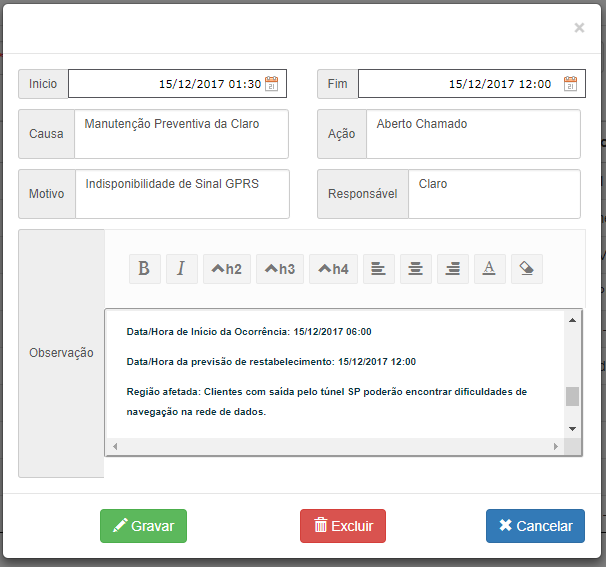
\includegraphics[width=0.5\linewidth]{images/33310_ANEXO_E_SIC_33310.png}
	\label{fig:e_sic_33310}
  \source{Resposta ao pedido de acesso a informação referente ao protocolo e-SIC 33310, 2017}
\end{figure}

\begin{table}[!htb]
\centering
\caption{Meta dados dos dados AVL da SPTrans}
\label{tab:avlDataset}
\begin{tabular}{c|c}
\hline
\textbf{Nome do campo} & \textbf{Descrição do campo} \\
\hline
\textit{cd\_evento\_avl\_movto} & 
Código sequencial identificador do evento \\
\hline
\textit{cd\_linha} & 
Código identificador da linha em operação
 \\
\hline
\textit{dt\_movto} & \begin{tabular}{@{}c@{}} Data da gravação em banco \\ de dados do evento gerado no AVL \end{tabular} \\
\hline
\textit{nr\_identificador} & 
Código identificador do AVL \\
\hline
\textit{nr\_evento\_linha} & 
Grupo de indicadores relacionados ao evento \\
\hline
\textit{nr\_ponto} & 
Código do ponto notável \\
\hline
\text{nr\_velocidade} & 
Velocidade instantânea \\
\hline
\textit{nr\_voltagem} & 
Tensão de alimentação \\
\hline
\textit{nr\_temperatura\_interna} & 
Temperatura do processador \\
\hline
\textit{nr\_evento\_terminal\_dado} & Código do evento relacionado no terminal de dados \\
\hline
\textit{nr\_evento\_es\_1} & 
Grupo de indicadores relacionados ao evento \\
\hline
\textit{nr\_latitude\_grau} & 
Latitude da geolocalização do veículo \\
\hline
\textit{nr\_longitude\_grau} & Longitude da geolocalização do veículo \\
\hline
\textit{nr\_indiceregistro} & 
Índice de geração do evento no AVL \\
\hline
\textit{dt\_avl} & 
Data da geração do evento no AVL \\
\hline
\textit{nr\_distancia} & \begin{tabular}{@{}c@{}} 
Distância em metros do evento com relação ao evento \\ anterior do mesmo AVL \end{tabular} \\
\hline
\textit{nr\_tipo\_veiculo\_geo} &
Código para identificação  no software de mapeamento \\
\hline
\textit{cd\_avl\_conexao} & \begin{tabular}{@{}c@{}} 
Código interno utilizado para  identificar
 \\   qual a conexão utilizada para transmissão do evento \end{tabular} \\
\hline
\textit{cd\_prefixo} & 
Prefixo do veículo \\
\hline
\end{tabular}
\end{table}


\chapter{Exploração e visualização de grandes volumes de dados}
\label{dataViz}

Este capítulo tem como objetivo apresentar uma arquitetura para visualizar e explorar grandes volumes de dados, a validação da arquitetura proposta é realizada com o Corpus AVL da SPTrans. Isso, porque além do grande volume esse conjunto de dados dados possui padrões complexos e demanda um sistema distribuído para serem processados, o qual é apresentado neste trabalho, capaz de suportar atividades analíticas, como visualização e exploração de dados. Tais análises, são importantes para o gerenciamento e planejamento do transporte público. Na seção \ref{related_work_data_viz} são mencionados alguns trabalhos referentes a visualização de de dados, encontrados por meio de uma revisão não sistemática da literatura; na \ref{druid} é descrita a arquitetura do banco de dados \textit{Druid}, principal componente da arquitetura proposta; na \ref{arch_viz} a arquitetura em questão para processamento e exploração dos dados AVL; na \ref{viz_case} os resultados obtidos no estudo de caso e, por fim, na \ref{viz_case_cons} as considerações finais.

\section{Trabalhos relacionados}
\label{related_work_data_viz}

Em \cite{chen2015survey} são mencionados conceitos básicos e fluxos de visualização de dados de tráfego (dos dados brutos, pré-processamento ao mapeamento visual, construído com símbolos visuais), além de uma visão geral das técnicas e métodos de processamento de dados relacionados para processar e descrever propriedades temporais, espaciais, numéricas e categóricas de dados de tráfego.

Analogamente, em \cite{andrienko2017visual} é descrita uma tipologia de dados de tráfego, capaz de abordar suas respectivas propriedades, problemas e transformações relevantes para a análise. Além disso, são apresentadas abordagens analíticas visuais para analisar dados de tráfego de veículos, pedestres, passageiros dentro de sistemas de transporte, etc.

Por fim, no trabalho desenvolvido em \cite{seraj2017aggregation} é apresentado um novo algoritmo para mapeamento de medições coletivas para monitorar as infraestruturas de transporte terrestre e, aliviar o impacto de imprecisões do \nomenclature{GPS}{Global Positioning System}{GPS} para monitoramento contínuo de infraestruturas de transporte por meio de \textit{smart phones}.

Nenhum dos trabalhos mencionados anteriormente aborda o uso de software livre com suporte a computação distribuída, escalabilidade, tolerância a falhas, processamento em tempo real, baixa latência e visualização de grandes volumes de dados temporais; o que é explorado neste trabalho usando banco de dados \textit{Druid} e o \textit{Apache Superset} para analisar padrões complexos existentes nos dados AVL da SPTrans.

\section{Druid}
\label{druid}

O Druid é um banco de dados para análises exploratórias em tempo real (latências abaixo da sub-segundos) em grandes conjuntos de dados. A arquitetura distribuída do Druid é composta por um \textit{cluster} com diferentes tipos de nós, que operam independentemente uns dos outros e possuem interação mínima entre eles. Existem duas dependências externas: (I) Apache Zookeeper\footnote{\url{https://zookeeper.apache.org}. Acessado em 23 de junho de 2018.}, responsável pela coordenação do cluster e (II) um sistema de gerenciamento de banco de dados relacional \nomenclature{RDBMS}{\textit{Relational Database Management Systems}}{(RDBMS --- \textit{Relational Database Management Systems}),} para armazenar parâmetros operacionais adicionais e configurações \cite{yang2014druid}.

\subsection{Real-time nodes}

\textit {Real-time nodes} são responsáveis por ingerir, indexar e consultar fluxos de eventos. Periodicamente, cada nó agenda uma tarefa em segundo plano para procurar todos os índices localmente persistentes, mesclando-os para construir \emph{blocos imutáveis de dados com todos os eventos ingeridos em um período de tempo}, conhecidos como \emph{segmentos}, os quais podem posteriormente serem carregados para uma camada de \textit {deep storage} \cite{yang2014druid}.

Durante os processos mencionados anteriormente não há perda de dados. Além disso, a imutabilidade dos blocos permite a consistência de leitura e um modelo de paralelização simples: \textit{historical nodes} podem simultaneamente examinar e agregar blocos imutáveis de forma não bloqueante \cite{yang2014druid}.

\subsection{Historical nodes}

Os \textit{historical nodes} são responsáveis por carregar, descartar e servir \emph{segmentos} imutáveis por meio de uma arquitetura \textit{shared-nothing} (sem um único ponto de contenção entre os nós) \cite{yang2014druid}.

\subsection{Broker nodes}

Os \textit{broker nodes} são responsáveis por receber consultas e mesclar resultados parciais dos \textit{historicals} e \textit{real-time nodes} antes de retornar um resultado final consolidado para o cliente \cite{yang2014druid}.

\subsection{Coordinator nodes}

Os \textit{coordinator nodes} são responsáveis pelo gerenciamento e distribuição dos dados nos \textit {historical nodes}, exigindo destes o carregamento, descarte e replicação dos dados \cite{yang2014druid}.

\section{Arquitetura utilizada para visualização e exploração dos dados AVL da SPTrans}
\label{arch_viz}

A Fig.~\ref{fig:viz_arch} mostra a arquitetura utilizada no estudo de caso deste capítulo, composta pelos componentes do \textit{Druid} em conjunto com o módulo \textit {Apache Superset}\footnote{\url{https://superset.incubator.apache.org}. Acessado em 23 de junho de 2018.} --- software de código aberto para exploração e análise de dados, nativamente integrado ao \textit{Druid}. Nesta arquitetura, dois fluxos para processamento de dados também são elencados: (I) \textit{batch} e (II) \textit{near real time}.

\begin{figure}[!htb]% H manda colocar exatamente nessa posição no texto (relativa aos parágrafos anterior e posterior)
	\centering
 	  \caption{Arquitetura usada no estudo de caso para visualização e exploração dos dados AVL da SPTrans}
		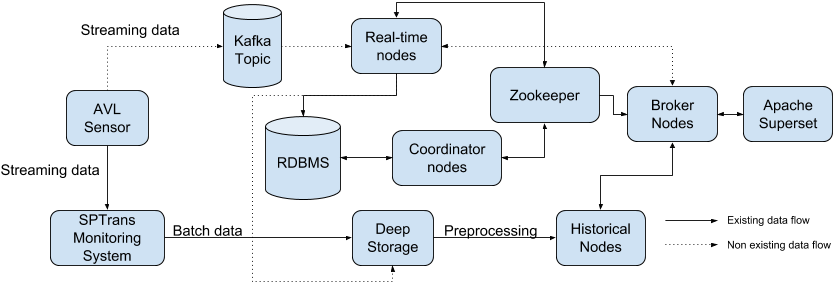
\includegraphics[width=1\linewidth]{images/viz_arch.png}
	\label{fig:viz_arch}
%  \source{Felipe Cordeiro Alves Dias, 2017}
\end{figure}

O fluxo de processamento em \textit{batch} é executado a partir dos dados extraídos do sistema de monitoramento da \textit{SPTrans}, ingeridos nos \textit{historical nodes} (a latência de ingestão máxima medida é 22914.43 eventos / segundo / núcleo, com uma fonte de dados com 30 dimensões e 19 métricas \cite{yang2014druid}) e disponibilizados para o \textit{Apache Superset} por meio dos \textit{broker nodes} (que tem uma latência média de consulta de aproximadamente 550 milissegundos \cite{yang2014druid}). É importante observar que o fluxo de processamento em \textit{batch} é o fluxo de dados implementado neste estudo de caso.

Na arquitetura ilustrada na Fig.\ref{fig:viz_arch}, o fluxo de dados em \textit{streaming} refere-se a uma proposta alvo para a \textit{SPTrans}, a fim de permitir a exploração e visualização dos dados dos ônibus da cidade de São Paulo em \textit{near real time}. Nesta proposta, os tópicos do \textit{Apache Kafka} desempenham o papel de receptores do fluxo de dados, a partir dos quais os dados podem seguir tanto o processamento em \textit{near real time} quanto \textit{batch}.

Ambos os fluxos de dados mencionados anteriormente são válidos, o fluxo \textit{streaming} não exclui a necessidade de um fluxo em \textit{batch}, o qual pode ser usado para análises mais complexas dos dados em questão. Além disso, é importante observar que em ambos os fluxos há um estágio de pré-processamento de dados, para adequar os dados AVL as especificações exigidas para a ingestão no \textit{Druid} (o que adiciona atraso no fluxo de processamento).

\section{Estudo de caso com os dados AVL da SPTrans}
\label{viz_case}

Grandes volumes de dados podem conter padrões complexos e difíceis de serem identificados. Devido a isso, é importante construir visualizações auxiliares para o processo de análise de dados. Com este propósito, usamos o \textit{Apache Superset}\footnote{\url{https://superset.incubator.apache.org}. Acessado em 29 de junho de 2018}, com suporte nativo ao \textit{Druid}, para exploração e visualização do \textit{corpus} da SPTrans. As figuras \ref{fig:analysis_by_bus_lines}, \ref{fig:pizza_bus}, \ref{fig:only_one_bus_map} e \ref{fig:buses_map} são exemplos de algumas visualizações construídas a partir dos dados de janeiro das linhas de ônibus selecionadas aleatoriamente.

A Fig. \ref {fig:analysis_by_bus_lines} ilustra uma série temporal referente à quantidade de dados enviados por ônibus selecionados aleatoriamente, referentes a janeiro de 2017. Com esta visualização é possível observar, por exemplo, a oscilação da quantidade de dados enviados, assim como os picos de maior e menor volume de envio de dados e janelas de tempo com dados ausentes, que podem indicar inúmeros problemas relacionados a essas viagens, como eventos de exceção.

\begin{figure}[!htb]% H manda colocar exatamente nessa posição no texto (relativa aos parágrafos anterior e posterior)
	\centering
 	  \caption{Quantidade de dados enviados por dia  por ônibus (selecionados aleatoriamente) em janeiro de 2017}
		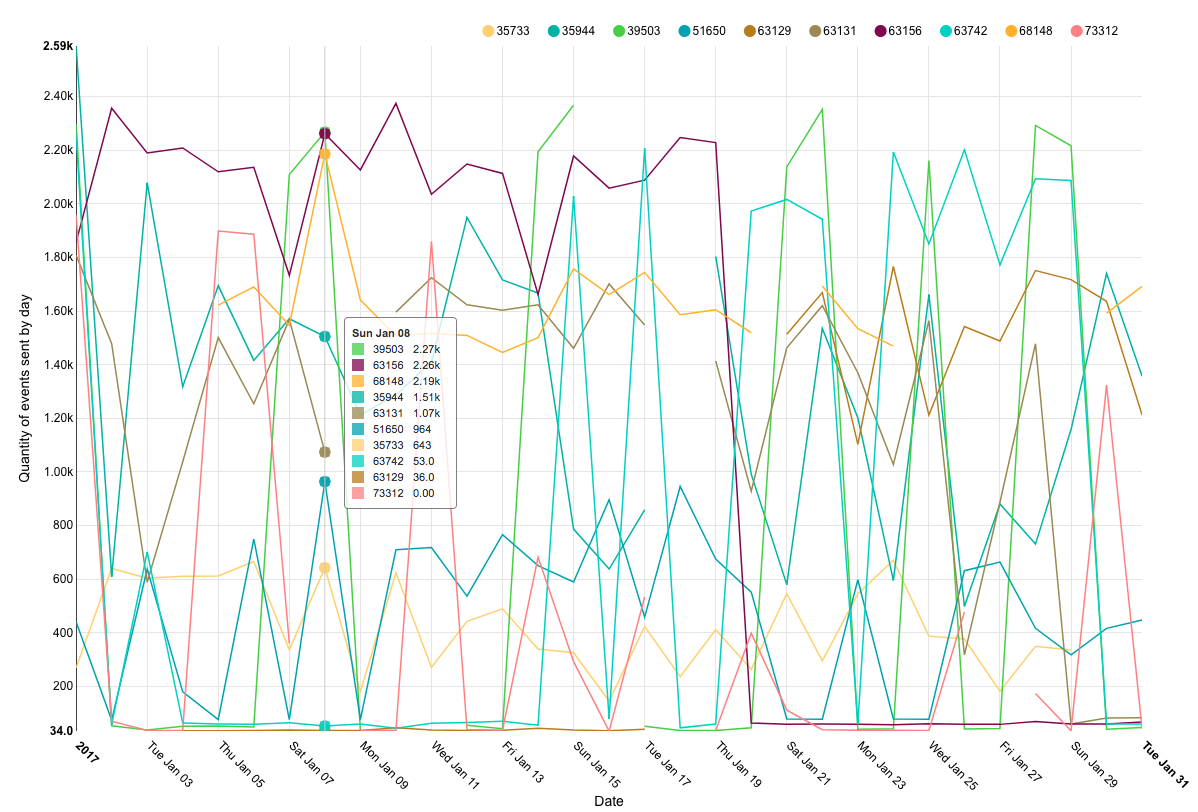
\includegraphics[width=1\linewidth]{images/analysis_by_bus_lines.png}
	\label{fig:analysis_by_bus_lines}
  %\source{Felipe Cordeiro Alves Dias, 2017}
\end{figure}

A Fig. \ref{fig:pizza_bus}, representa a distribuição dos dados enviados em janeiro, a partir de uma amostra aleatória. Nessa figura é possível analisar que a distribuição da quantidade de dados enviados não é normalizada, ou seja, existem ônibus que normalmente enviam mais dados do que os demais. Há muitas razões possíveis para isso, por exemplo: viagens de ônibus mais longas que outras, regiões com diferenças climáticas; módulos AVL desatualizados; maior quantidade de ônibus em uma determinada linha, etc.

\begin{figure}[!htb]% H manda colocar exatamente nessa posição no texto (relativa aos parágrafos anterior e posterior)
	\centering
 	  \caption{Distribuição da quantidade de dados enviados por ônibus (selecionados aleatoriamente) em janeiro de 2017}
		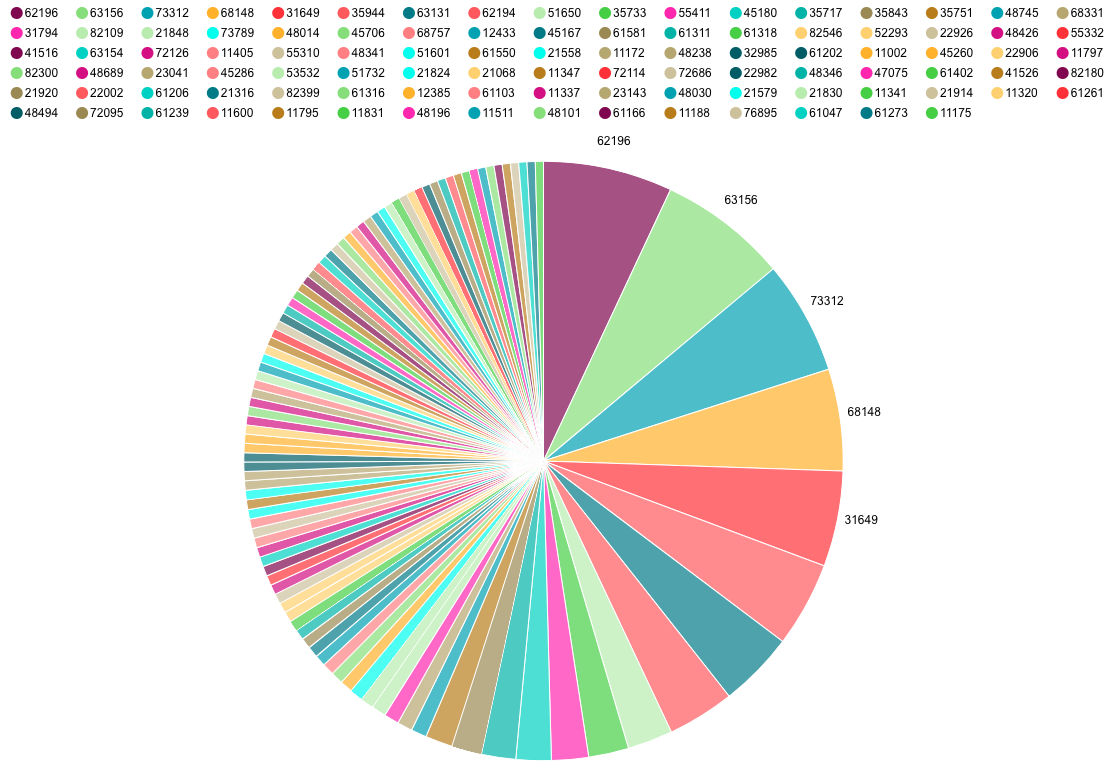
\includegraphics[width=1\linewidth]{images/pizza_bus.png}
	\label{fig:pizza_bus}
  %\source{Felipe Cordeiro Alves Dias, 2017}
\end{figure}

Finalmente, os mapas exibidos pelas figuras \ref {fig:buses_map} e \ref{fig:only_one_bus_map} ajudam a identificar a localização a partir da qual os dados estão sendo enviados, permitindo visualizar possíveis pontos de falhas durante a transmissão desses dados. O primeiro mapa, respectivamente, refere-se à rota de uma única linha de ônibus e o segundo de todas as rotas; em ambos os casos, referentes aos dados de janeiro. Além disso, na figura \ref {fig:buses_map}, é possível observar a segregação urbana da cidade, devido ao fato de algumas regiões terem uma maior densidade de dados enviados, o que também indica regiões de maior tráfego, nas quais eventos de exceção teriam maior impacto.

\begin{figure}[!htb]% H manda colocar exatamente nessa posição no texto (relativa aos parágrafos anterior e posterior)
	\centering
 	  \caption{Localizações enviadas em Janeiro de 2017 de uma linha de ônibus selecionada aleatoriamente}
		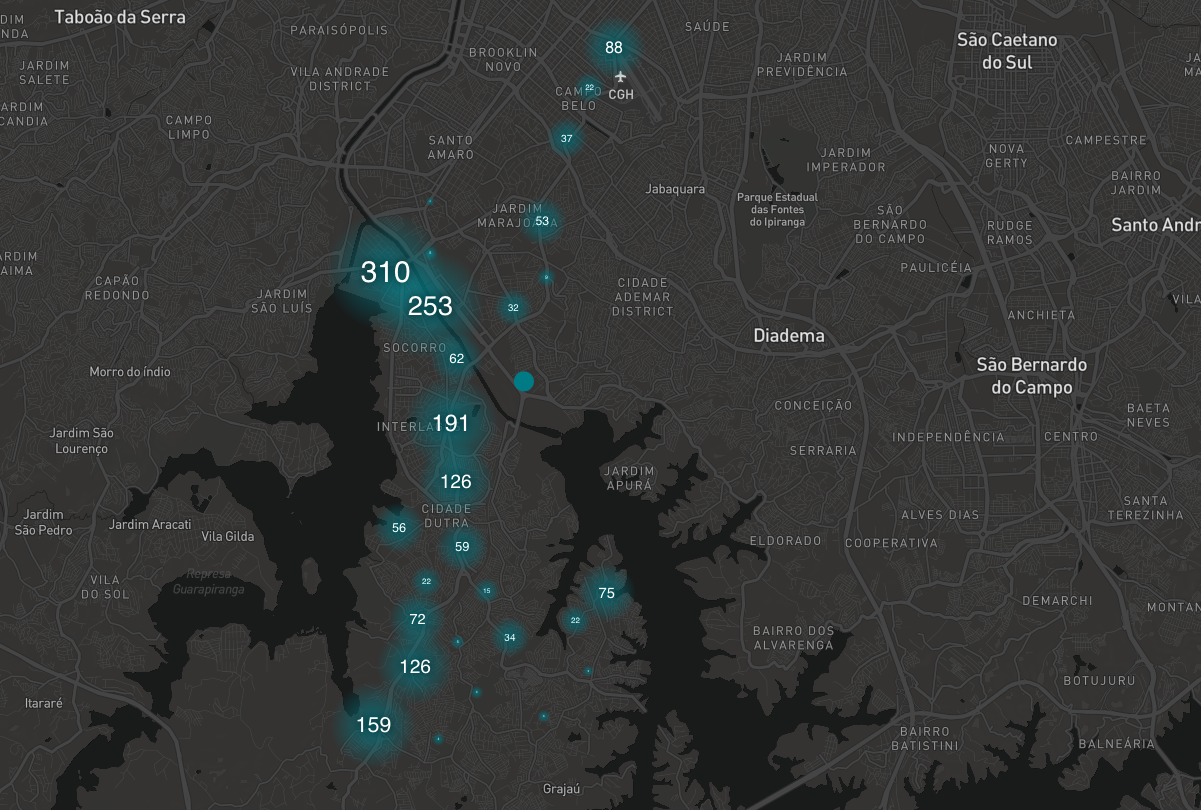
\includegraphics[width=0.95\linewidth]{images/only_one_bus_map.png}
	\label{fig:only_one_bus_map}
  %\source{Felipe Cordeiro Alves Dias, 2017}
\end{figure}

\begin{figure}[!htb]% H manda colocar exatamente nessa posição no texto (relativa aos parágrafos anterior e posterior)
	\centering
 	  \caption{Localizações dos ônibus referente a movimentação de Janeiro de 2017}
		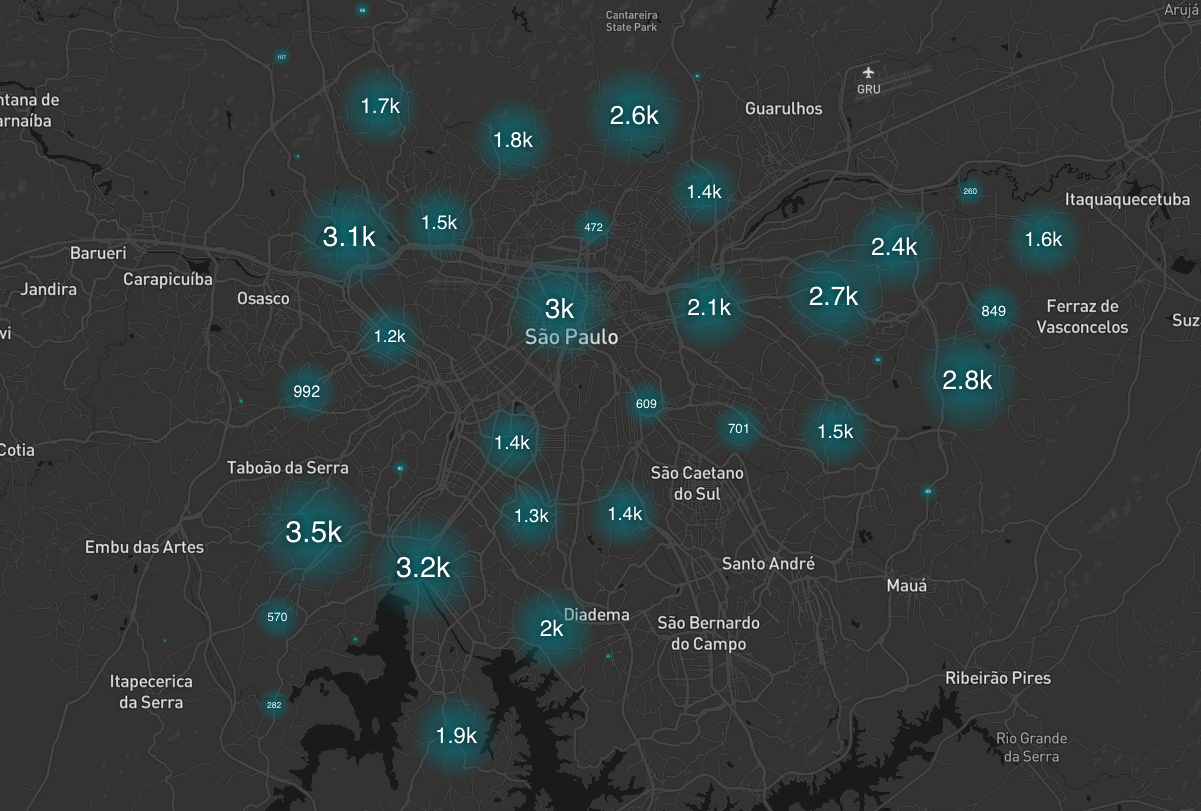
\includegraphics[width=0.95\linewidth]{images/buses_map.png}
	\label{fig:buses_map}
\end{figure}

\section{Consideração sobre a arquitetura utilizada para exploração e visualização dos dados AVL da SPTrans}
\label{viz_case_cons}

Este capítulo apresentou um estudo de caso relacionado à visualização de grandes conjuntos de dados, utilizando dados dos ônibus da cidade de São Paulo. Também, mostramos que é possível encontrar padrões complexos e incomuns e possíveis eventos de exceção em grandes conjuntos de dados por meio da visualização. O \textit{Druid} e o \textit{Apache Superset} demonstraram suporte a agregação, exploração e visualização de grandes conjuntos de dados. Como trabalho futuro, pretendemos implementar o fluxo de dados mencionado na Fig.~\ref{fig:viz_arch}, em um cenário de exploração e visualização de dados \textit{near real time}.


\chapter{Uma metodologia baseada em \textit{tweets} para encontrar linhas de ônibus impactadas por eventos de exceção na cidade de São Paulo}
\label{exp1}

Nesta seção é apresentada uma metodologia baseada em \textit{tweets} para identificar linhas de ônibus impactadas por eventos de exceção. De acordo com a Fig. \ref{fig:tweet_based_methodology}, a metodologia, explicada em detalhes na seções seguintes, é composta por:
\begin{enumerate*}
\item Uma base de dados de \textit{tweets} --- \textit{Copus Twitter}.
\item Pré-processamento dos \textit{tweets} existentes no conjunto de dados.
\item Extração de localização e geolocalização.
\item Processamento dos \textit{tweets}.
\item Criação de um modelo de classificação de \textit{tweets} em classes de eventos de exceção.
\item Identificação das linhas impactadas --- por meio de consultas a base GTFS existente no \textit{Corpus SPTrans} --- a partir de um raio de cada evento de exceção.
\end{enumerate*}

\begin{figure}[!htb]
	\centering
 	  \caption{Metodologia baseada em \textit{tweets} para encontrar linhas de ônibus impactadas por eventos de exceção na cidade de São Paulo}
		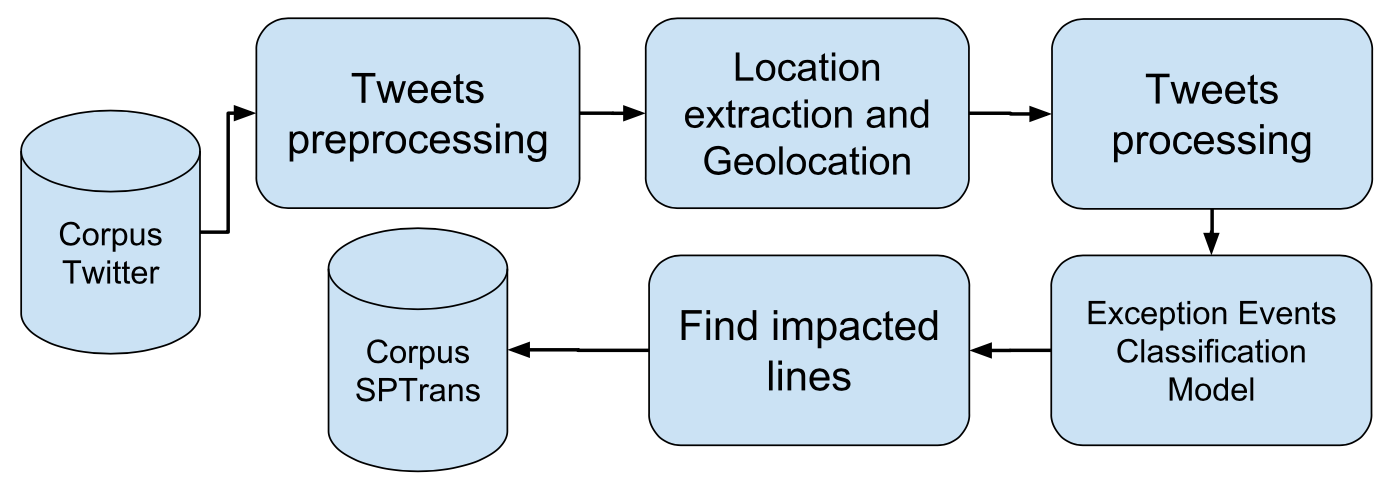
\includegraphics[width=0.7\linewidth]{images/tweet_based_methodology.png}
	\label{fig:tweet_based_methodology}
\end{figure}

\section{Pré-processamento}
\label{preprocessing}

Numa pré-análise do \textit{Corpus Twitter}, podemos afirmar que os \textit{tweets} publicados pelos \textit{profiles} selecionados evitam o uso de gírias, abreviações, erros de digitação; conforme consta nos \textit{tweets} de exemplo contidos no trecho de código em \textit{json}, no apêndice \ref{tweetsSample}.  Isso diferencia tais \textit{tweets} dos \textit{tweets} publicados por usuários comuns do \textit{Twitter}, que contém erros gramaticais, de sintaxe e que normalmente dependem de análise contextual para que possam ser interpretados.

Apesar disso, com base na literatura analisada (\cite{Steiger2015Census}, \cite{Middleton2014}, \cite{Kobdani2010}, \cite{Setiawan2017},  \cite{Zagal2016}), as seguintes etapas de pré-processamento são necessárias para remoção de ruído e redução da dimensão do espaço de \textit{features} e foram realizadas para o \textit{Corpus Twitter}:

\begin{itemize}
\item \textit{Case folding}: processamento de normalização de todas as letras do texto (de a-z) para minúsculas.
%\item \textit{\textbf{Tokenization}}: processamento realizado para obtenção das palavras  (\textit{tokens}) que compõem uma sentença, inclui a remoção de números, pontuações e caracteres que não pertencem ao alfabeto \cite{Setiawan2017}.  
%\item \textbf{Remoção de} \textit{\textbf{stopwords}}: processamento para remoção do conjunto de \textit{tokens} de palavras sem significado ou importância \cite{Setiawan2017}, o que reduz a quantidade de ruído do conteúdo \textit{tweet} \cite{Steiger2015Census}.
%\item \textit{\textbf{Stemming}}: processamento para encontrar a raiz de uma palavra, removendo sufixos e prefixos (no caso do Português Brasileiro) das palavras derivadas \cite{Setiawan2017}.
\item Remoção \nomenclature{URL}{\textit{Uniform Resource Locator}} \textit{URLs} e menções a outros \textit{tweets}.
\item Remoção de acentos, \textit{emoticons} e pontuações substituídas por espaços vazios.
%\item Correção erros de digitação por meio de uma função de mapeamento
\item \textit{Stemming} --- realizado neste trabalho na fase de processamento mencionada na subseção \ref{processing}, com o objetivo de não afetar o processo de extração de endereços. 
\end{itemize}

Além disso, é importante observar que (I) as informações referentes a data e hora mencionadas no conteúdo dos \textit{tweets} (\textit{stopwords} específicas do domínio) são removidas do texto original. As informações de data e hora consideradas para os eventos de exceção são as contidas nos meta dados dos \textit{tweets}, posto que ao analisarmos os \textit{tweets} verificamos que as informações de data e hora contidas no texto normalmente são referentes a eventos futuros, os quais não são considerados por este trabalho; (II) os \textit{retweets} não estão presentes no \textit{Corpus Twitter}; (III) no pré-processamento não há transformação do conteúdo dos \textit{tweets}, embora trabalhos como os relacionados a identificação de sentimentos usem esse meio para transformar \textit{emoticons} nos sentimentos que eles representam \cite{Zagal2016}; (IV) as \textit {hashtags} não são removidas dos \textit{tweets} originais, pois são importantes para a classificação dos eventos de exceção.

Uma atenção especial foi dada às \textit{hashtags}, que são relevantes para a classificação de eventos de exceção, mas adicionam ruído à fase de extração de endereços. Para mitigar o problema, \textit{hashtags} são identificados e substituídos por espaços vazios no processo de extração de endereço. Além disso, é importante notar que as \textit{hashtags} não são removias dos \textit{tweets} originais.

\section{Extração de endereço e geolocalização}

Analisando o conteúdo dos \textit{tweets} das contas selecionadas, é possível observar que os textos publicados seguem um determinado padrão e, portanto, são na verdade semi-estruturados. Ante a isso, usamos a seguinte expressão regular para extrair os endereços presentes no conteúdo dos \textit{tweets}:
%
\begin{equation}
ER = \lbrace L_1 | S_1 | L_2 | S_2 | \dots | L_n | S_n \rbrace \lbrace [a-z\grave{A}-\ddot{y}\_] + \rbrace
\end{equation}

A expressão anterior é dividida em dois conjuntos, no primeiro ($\lbrace L_1 | S_1 | L_2 | S_2 | \newline \dots | L_n | S_n \rbrace $), (L --- logradouros) e (S --- acrônimos de espaços públicos) são concatenados para especificar um filtro e identificar sequências inicializadas com espaços públicos ou seus respectivos acrônimos. No segundo conjunto ($\lbrace [a-z\grave{A}-\ddot{y}\_] + \rbrace $), é especificado um filtro para identificar um conjunto de palavras após L ou S, que são candidatas a compor o endereço desejado.

Essas palavras são candidatas porque é difícil saber quantas palavras após L ou S pertencem ao endereço, no entanto, as contas selecionadas publicam padrões visíveis após os endereços. Como consequência, um método possível para encontrar o endereço desejado é a remoção desses padrões após o início do endereço.

Após a extração do endereço, é necessário geolocalizar o endereço encontrado --- apenas 1,5 \% de \textit {tweets} têm geolocalização \cite{niu2016community} --- o que é possível, por exemplo, usando a \nomenclature{API}{\textit{Application Programming Interface}}{API} de geocodificação do Google Maps\footnote {\url {https://developers.google.com/maps/documentation/geocoding}. Acessado em 11 de Abril de 2018.}. Os parâmetros de URL utilizados neste trabalho para chamar a API mencionada anteriormente são: (I) \emph {address} --- o endereço desejado; (II) \emph {bounds} --- uma caixa delimitadora para o resultado retornado, a qual é especificada pelas coordenadas de latitude / longitude dos cantos sudoeste e nordeste de São Paulo; (III) \emph {region} --- código da região com dois caracteres, por exemplo, \textit{br} para o Brasil e (IV) \emph {token} --- \textit{token} usado na autenticação da API.

Em seguida, a resposta HTTP é processada para obter os valores da localização (que contém informações de latitude e longitude) e o \emph{endereço formatado}. É importante observar que os \textit{tokens} do endereço extraído (\emph{endereço não formatado}) são \textit{stopwords} específicas do \textit{corpus} em caso de alta frequência de eventos de exceção localizados neste endereço, devido ao fato de que nesse cenário elas são tratados como \textit{features} relevantes para o modelo de classificação. Portanto, os \textit{tokens} dos endereços extraídos são armazenados para serem removidos na fase de processamento dos \textit{tweets}.

\section{Processamento de \textit{tweets}}
\label{processing}

Nesta fase, os \textit {tweets} são preparados para serem usados para treinar um modelo de classificação de eventos de exceção; neste momento, todos os \textit {tweets} já foram pré-processados. Conforme mencionado na seção anterior, nesta fase, os \textit{tokens} dos endereços extraídos armazenados são removidos para redução de ruído e as \textit{stopwords} do Português Brasileiro filtradas\footnote{\textit{Stopwords} do Português Brasileiro obtidas da \nomenclature{NLTK}{Natural Language Toolkit}{NLTK ---} \url{https://www.nltk.org}. Acessado em 19 de Abril de 2018.} e todos os demais \textit{tokens}  processados por um \textit{stemmer} para o  Português Brasileiro\footnote{RSLP Stemmer --- \url {http://www.nltk.org/\_modules/nltk/stem/rslp.html}. Acessado em 19 de Abril de 2018.} para reduzir a dimensão do espaço de \textit{features}.

\section{Classificação manual do Corpus \textit{Twitter}}
\label{manualClassification}

Encontrar eventos de exceção envolve a identificação de eventos relacionados a uma exceção, o que é possível por meio de classificação de \textit{tweets} (manualmente ou de forma autônoma). De acordo com a revisão sistemática realizado no Capítulo \ref{revisao}, as seguintes classes podem ser usadas para classificar eventos de exceção:

\begin{enumerate}
\item \textbf{Acidentes}.
\begin{enumerate}
\item Acidentes nas estações transporte \cite{Itoh2016}.
\item Incêndio \cite{Itoh2016}.
\end{enumerate}

\item \textbf{Espaço-temporais}.
\begin{enumerate}
\item Dia da semana \cite{Chen2016}.
\item Hora do dia \cite{Chen2016}.
\end{enumerate}

\item \textbf{Eventos sociais}.
\begin{enumerate}
\item Feiras de rua \cite{Chen2016}.
\item Festivais \cite{Chen2016}, \cite{Lecue2014}.
\item Jogos esportivos \cite{Chen2016}, \cite{Gal-Tzur2014}.
\item Passeatas e maratonas \cite{Chen2016}, \cite{Itoh2016}.
\end{enumerate}

\item \textbf{Eventos urbanos}.
\begin{enumerate}
\item Relacionados ao tráfego \cite{Chen2016}, \cite{Lecue2014}.
\end{enumerate}

\item \textbf{Desastres naturais}.
\begin{enumerate}
\item Tempestades \cite{Itoh2016}.
\item Terremoto \cite{Itoh2016}.
\item Tufões \cite{Itoh2016}.
\end{enumerate}

\item \textbf{Metereológicos}.
\begin{enumerate}
\item Dia claro, nublado, chuvoso, nevando, com neblina \cite{Chen2016}.
\item Temperatura do ar \cite{Chen2016}.
\end{enumerate}
\end{enumerate}

Após o estudo do domínio do conhecimento, por meio da revisão sistemática para coletar as classes de exceção, o Corpus Twitter, contendo 60.985, foi classificado manualmente de acordo com suas respectivas classes. Tal conjunto foi usado para treinar o modelo de classificação de \textit{tweets} em classes de eventos de exceção. 

\section{Modelo de classificação de \textit{tweets} relacionados a eventos de exceção}
\label{model}

O corpus obtido da fase de processamento de \textit {tweets} é representado por meio de um \textit{bag-of-words}, que contém vetores de \textit{features} criados usando a medida \textit{Term Frequency - Inverse Document Frequency}\nomenclature{TF-IDF}{\textit{Term Frequency - Inverse Document Frequency}} (TF-IDF). A bag-of-words é particionada aleatoriamente em conjuntos de treinamento (60\%) e teste (40\%), os quais são entradas para os algoritmos de classificação mencionados na subseção ~\ref{supervisionedLearning}.

\section{Encontrando linhas de ônibus afetadas por eventos de exceção}

Para encontrar as linhas de ônibus afetadas por eventos de exceção, é necessário correlacionar latitude e longitude dos eventos de exceção com as \textit{stops} da GTFS da SPTrans. Como mencionado anteriormente, os dados referentes as \textit{stops} contém os locais individuais em que os veículos pegam ou deixam passageiros, incluindo coordenadas de latitude e longitude.

De acordo com a seção~\ref{CorpusSPTrans}, todas as coordenadas são armazenadas em pares no formato \textit{legacy} e em coleções com índices geoespaciais. Assim, é possível usar a função \textit{\$near} do MongoDB\footnote {\url{https://docs.mongodb.com/manual/reference/operator/query/near}. Acessado em 18 de Maio de 2018.} para encontrar as \textit{stops} próximas às coordenadas do evento de exceção. Como consequência da GTFS, o \textit{stop\_id} faz parte dos atributos contidos no arquivo de \textit{stops}, referindo-se a um código de parada de ônibus com o qual é possível correlacioná-lo com as bases \textit{stop\_times} e \textit{lines} (por meio do atributo \textit{trip\_id} existente em \textit{stops}) para obter mais detalhes sobre a direção da linha de ônibus, identificação, etc.

\section{Resultados}
	
A metodologia foi aplicada ao Corpus Twitter\footnote{Conjunto de dados disponível em: \url{https://drive.google.com/drive/folders/16NIevLsBR0A45UHdPDvv2lZZx6gF4R0p?usp=sharing}. Acessado em 8 de Setembro de 2018.}. No final do pré-processamento e processamento dos \textit{tweets}, o corpus obteve 3.761.226 palavras, com um vocabulário de 33 palavras. O comprimento máximo das sentenças do conjunto de dados é 136, sua respectiva variação é ilustrada pela Figura ~\ref{fig:corpus_metrics}.
 
\begin{figure}[!htb]
	\centering
 	  \caption{Histograma da variação dos tamanhos das sentenças dos \textit{tweets} existentes no \textit{Corpus Twitter}}
		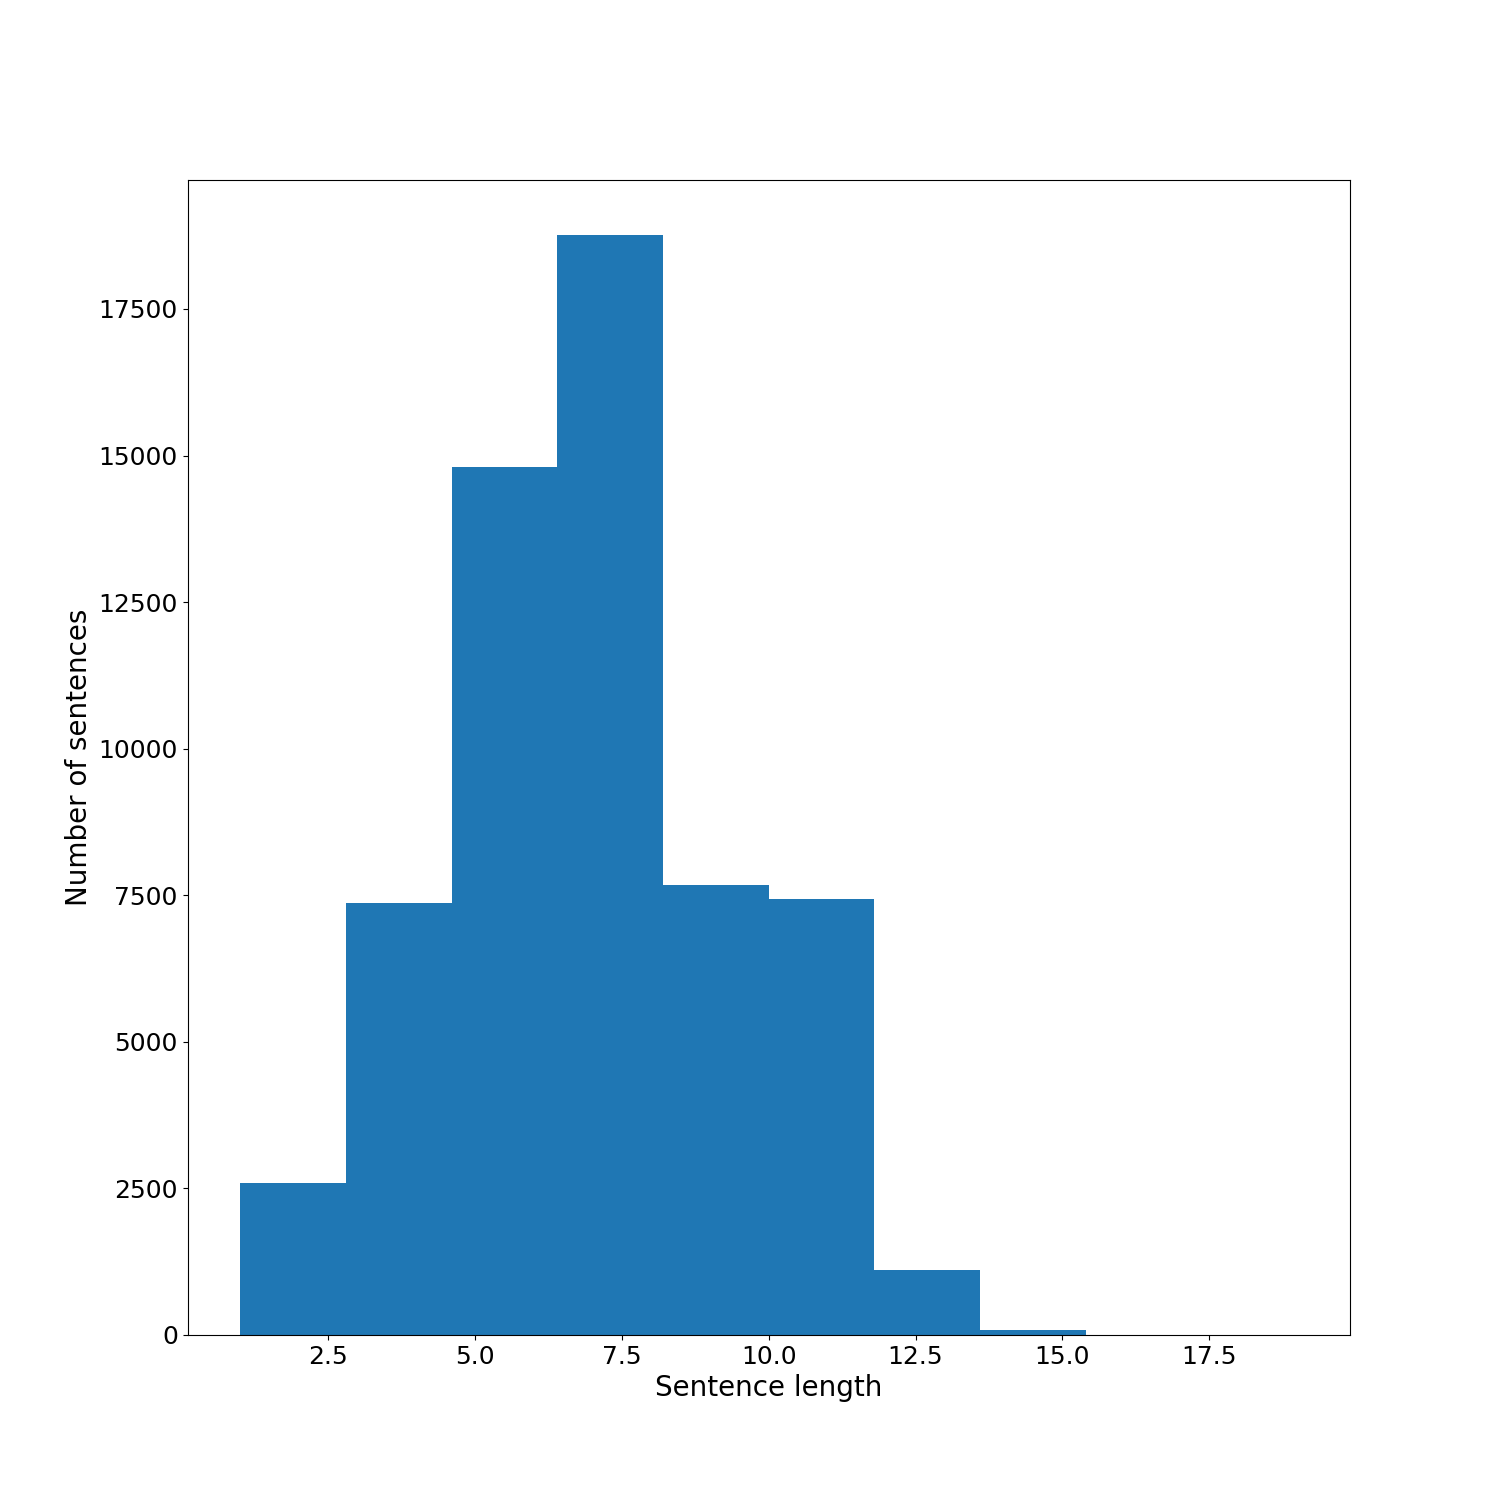
\includegraphics[width=1\linewidth]{images/corpus_metrics.png}
	\label{fig:corpus_metrics}
\end{figure}

Todos os \textit{tweets} existentes no \textit{Corpus Twitter} foram classificados manualmente de acordo com os eventos de exceção identificados. Este conjunto de dados é composto pelas seguintes classes: Acidente, Irrelevante --- quando o \textit{tweet} não é um evento de exceção, Desastre Natural, Evento Social e Evento Urbano. A figura \ref{fig:tweets_distribution} ilustra a distribuição das classes de eventos de exceção em cada conta selecionada.

\begin{figure}[!htb]
	\centering
 	  \caption{Distribuição das classes dos eventos de exceção do Corpus Twitter}
		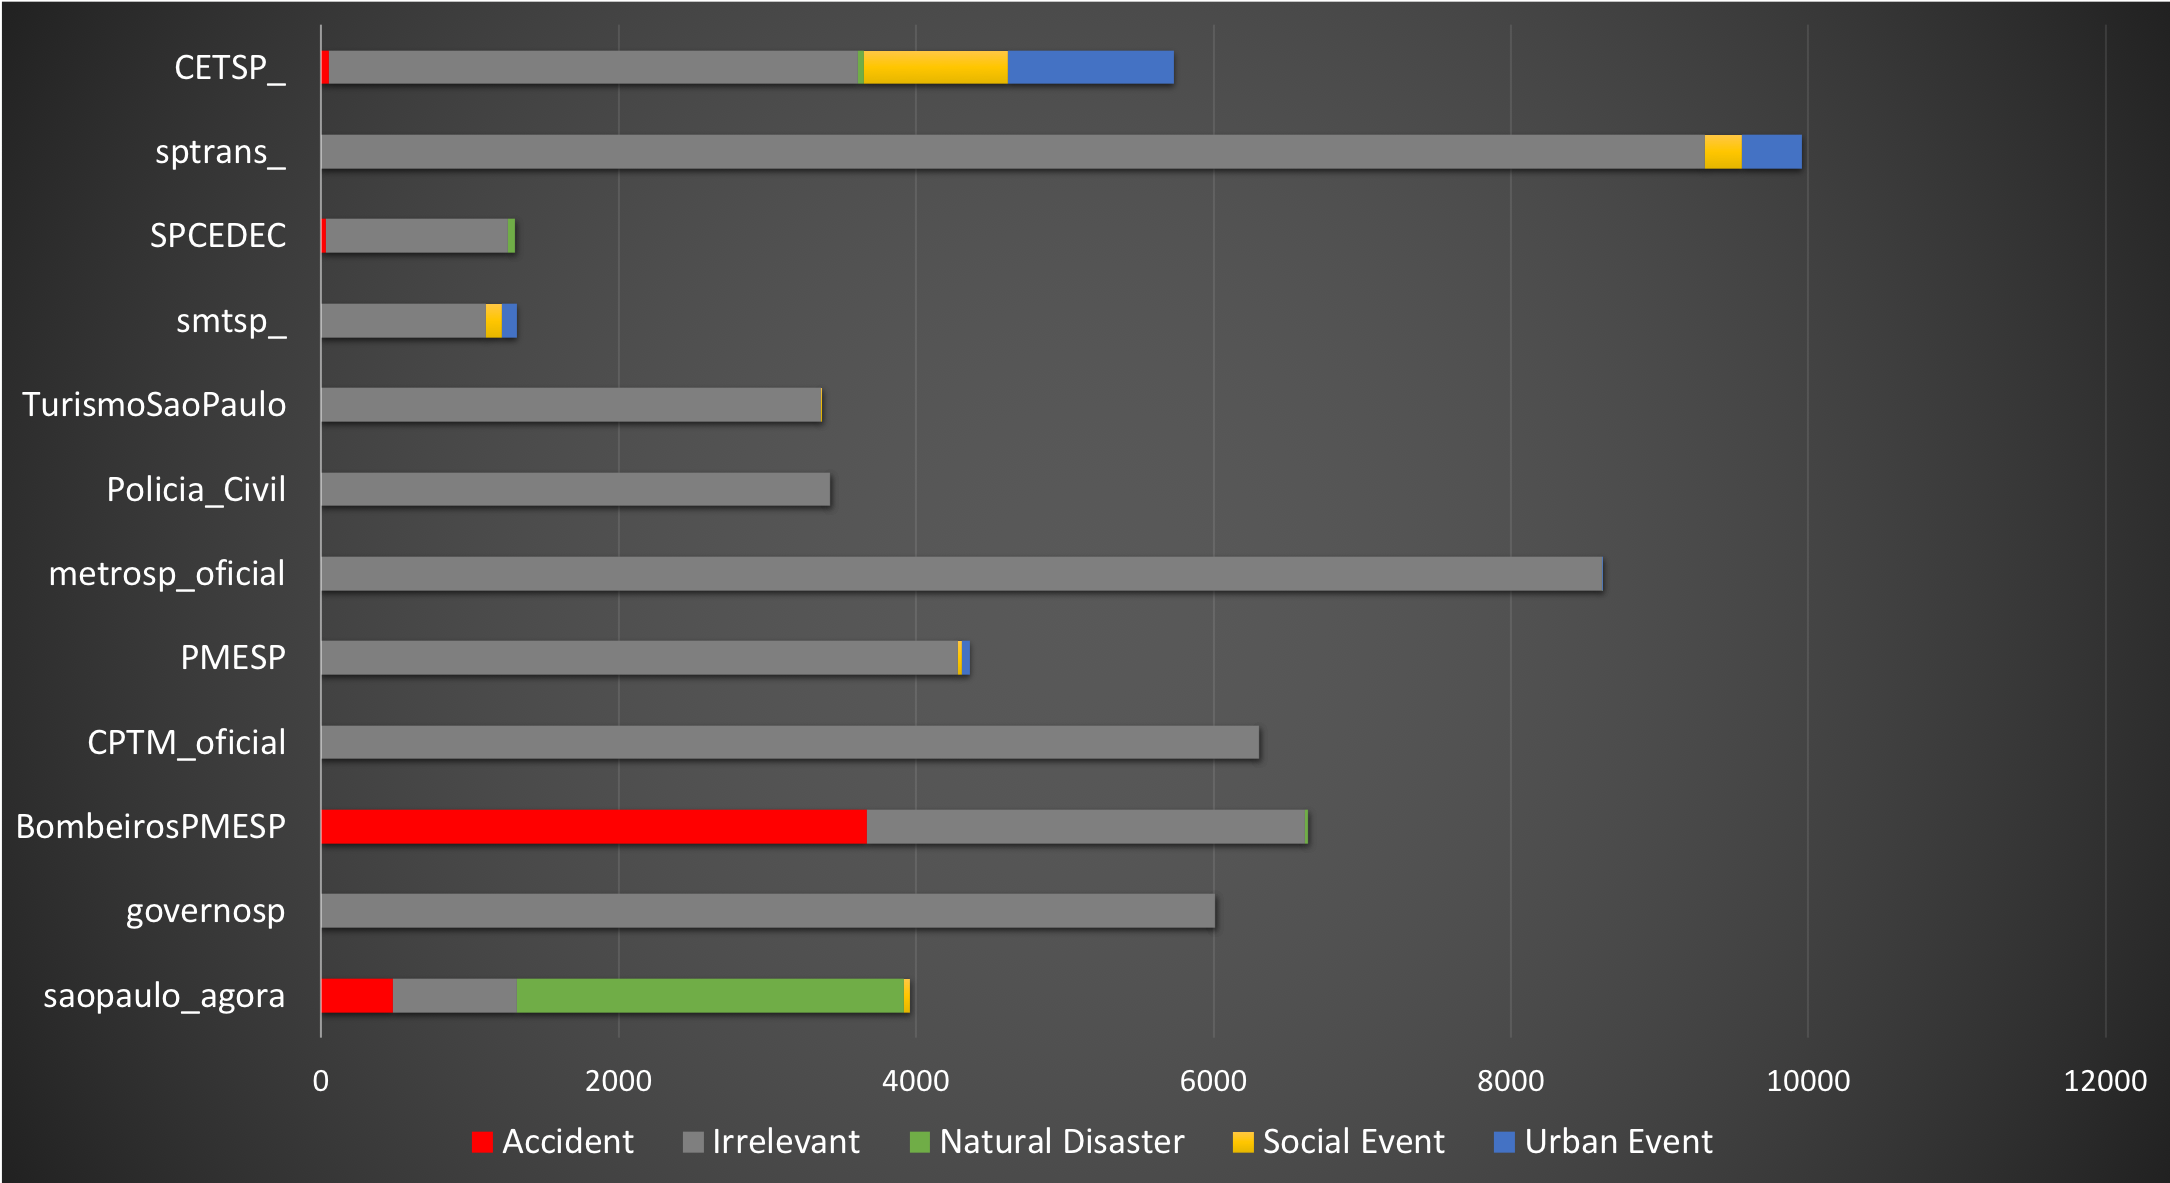
\includegraphics[width=1\linewidth]{images/tweets_distribution.png}
	\label{fig:tweets_distribution}
\end{figure}

Esse conjunto de dados rotulado foi usado para treinar modelos de classificação de eventos de exceção, com base em uma \textit{bag-of-words}, descrita na Seção ~\ref{model}. De acordo com a Tabela ~\ref{tab:metrics}, o modelo que usa o algoritmo \textit{Multi-layer Perceptron} para classificação é mais adequado para a tarefa de classificar os \textit{tweets} em eventos de exceção. A matriz de confusão relacionada ao algoritmo de \textit{Multi-layer Perceptron} é ilustrada pela Figura ~\ref{fig:confusion_matrix_mpc}, as matrizes de confusão dos demais algoritmos podem ser consultadas no apêndice \ref{apendiceE}.

\begin{table}[!htb]
\centering
\caption {Métricas das avaliações dos algoritmos utilizados para classificação dos \textit{tweets} em eventos de exceção}
\label {tab:metrics}
\begin{tabular}{c|c|c|c|c}
\hline
\textbf{Algoritmo} & \textbf{Acurácia} & \textbf{Precisão} & \textbf{Revocação} & \textbf{\textit{f1-score}} \\
\hline
\textit{Decision Tree} & 0.966 & 0.966 & 0.966 & 0.966 \\
\hline
\textit{Gaussian Naive Bayes} & 0.891 & 0.919 & 0.891 & 0.901 \\
\hline
\textit{K-Nearest Neighbors} & 0.970 & 0.971 & 0.970 & 0.970 \\
\hline
\textit{Logistic Regression} & 0.970 & 0.970 & 0.970 & 0.969 \\
\hline
\textit{Multi-layer Perceptron} & \textit{0.974} & \textit{0.974} & \textit{0.974} & \textit{0.974} \\
\hline
\textit{Multinomial Naive Bayes} & 0.954 & 0.953 & 0.954 & 0.951 \\
\hline
\textit{Random Forest} & 0.972 & 0.971 & 0.972 & 0.971 \\
\hline
\textit{Support Vector Machine} & 0.828 & 0.686 & 0.828 & 0.751 \\
\hline
\end{tabular}
\end{table}


\begin{figure}[!htb]
	\centering
 	  \caption{Matriz de confusão relacionada a classificação dos \textit{tweets} em eventos de exceção por meio do algoritmo \textit{Multi-layer Perceptron}}
		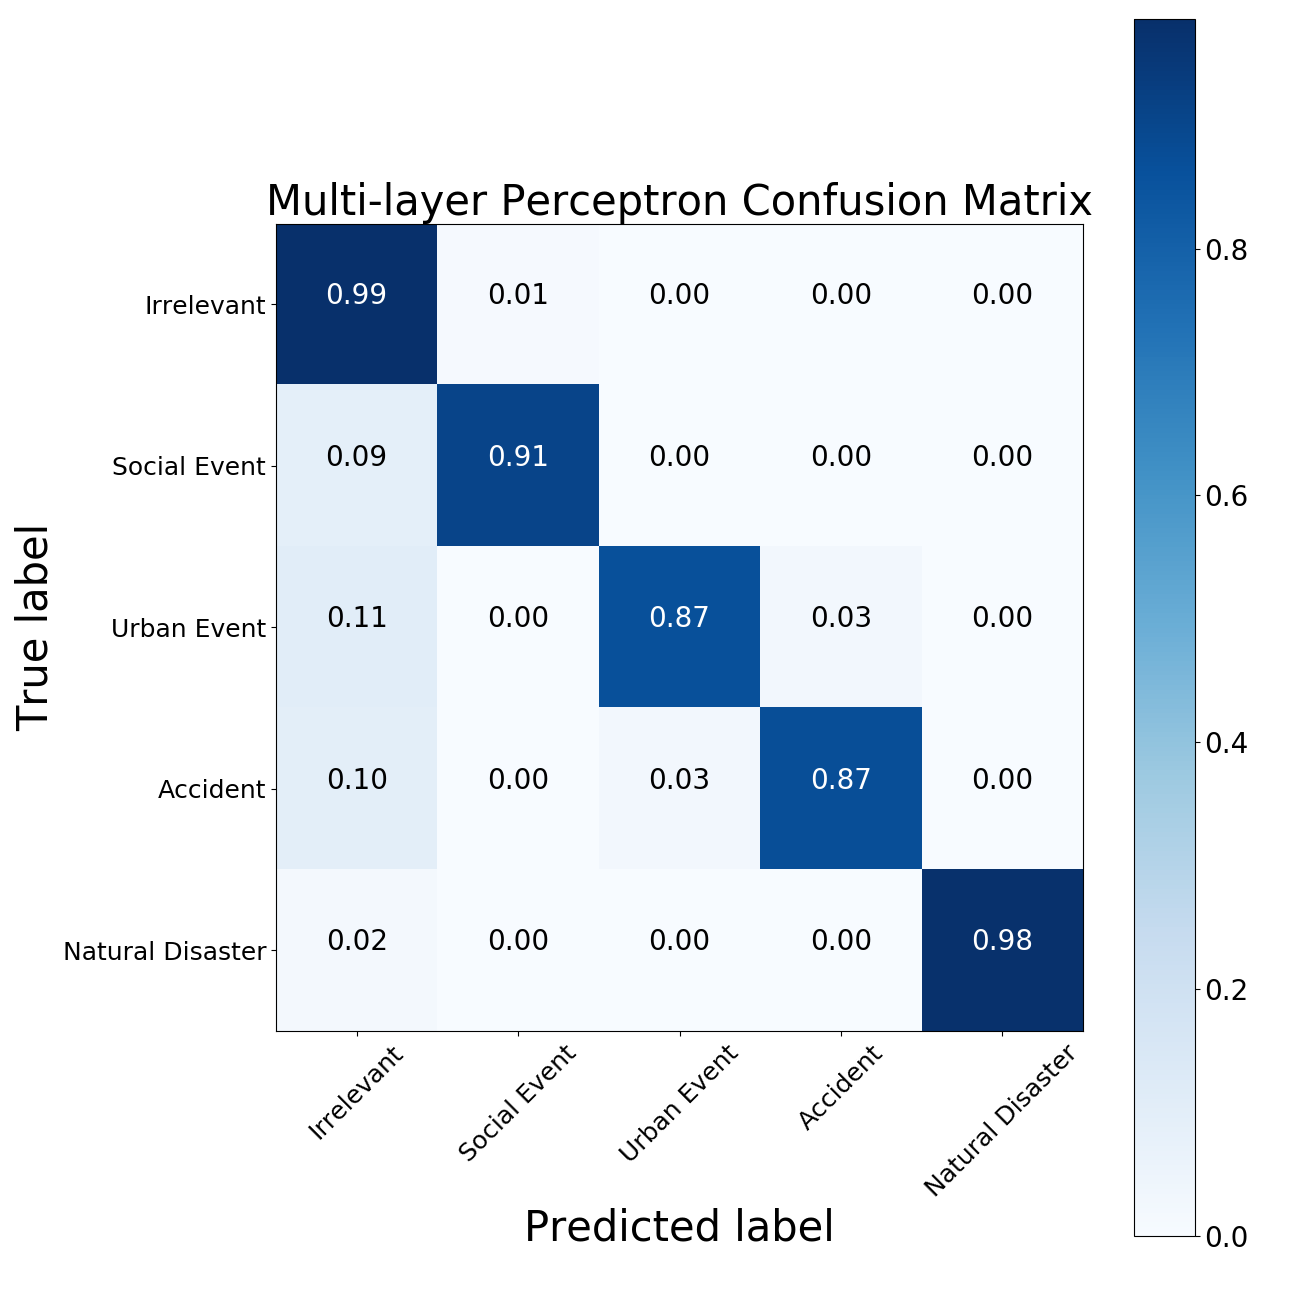
\includegraphics[width=1\linewidth]{images/confusion_matrix_mpc.png}
	\label{fig:confusion_matrix_mpc}
\end{figure}

Dos 60.984 \textit{tweets} 10.027 foram classificados em eventos de exceção e desse subconjunto encontrados 7.674 endereços, de acordo com a Tab. \ref{tab:qtdExtractedAddresses} --- desconsiderando o tipo de localidade \textit{APPROXIMATE} --- (o que representa 76,53\% do total dos \textit{tweets} eventos de exceção, sem considerar a classe \textit{Irrelevant}). A quantidade de endereços extraídos por classe está descrita na Tab. \ref{tab:qtdExtractedAddresses}, as razões para \textit {tweets} sem endereço extraído são:

\begin{enumerate*}
\item \textit{Tweets} apenas com o ponto de interesse, ou seja, não consta explicitamente o endereço.
\item \textit{Tweets} sem informação de endereço.
\item \textit{Tweets} com nome de logradouro incomum (por exemplo \emph{passagem}, \emph{complexo viário}, \emph{ligação sentido}).
\item \textit{Tweets} com endereços com palavras concatenadas (por exemplo \emph{avenidapaulista}).
\end{enumerate*}

Os \textit{tipos de localidades}\footnote{Disponível em \url{https://developers.google.com/maps/documentation/geocoding}. Acessado em 16 de setembro de 2018.} podem ser classificados em:
\begin{enumerate*}
\item \textit{ROOFTOP} --- Indica que o resultado retornado há informações de localização com precisão a nível do endereço de rua.
\item \textit{RANGE\_INTERPOLATED} --- Indica que o resultado retornado reflete uma aproximação interpolada entre dois pontos precisos (como interseções). Geralmente, os resultados interpolados são retornados quando os códigos geográficos do \textit{rooftop} não estão disponíveis para um endereço de rua.
\item \textit{GEOMETRIC\_CENTER} --- Indica que o resultado retornado é o centro geométrico de um resultado.
\item \textit{APPROXIMATE} --- Indica que o resultado retornado é aproximado.
\end{enumerate*}

Neste estudo de caso, desconsideramos os endereços com classificação \textit{APPROXIMATE}, devido ao fato de poderem comprometer a confiabilidade das análises realizadas. 

\begin{table}[!htb]
\centering
\caption {Quantidade de eventos extraídos por classe}
\label {tab:qtdExtractedAddresses}
\begin{threeparttable}
\begin{tabular}{c|c|c|c|c|c}
\hline
\textbf{Classe} & \textbf{\#endereços extraídos\tnote{a}} & \textbf{\textit{\#APP\tnote{b}}} & \textbf{\textit{\#GEO\tnote{c}}} & \textbf{\textit{\#RANGE\tnote{d}}} & \textbf{\textit{\#ROOF\tnote{e}}} \\
\hline
Accident & 3.439 & 7 & 805 & 1.130 & 1.497 \\
\hline
Irrelevant & 451 & 13 & 292 & 6 & 140 \\
\hline
Natural Disaster & 2.464 & 9 & 340 & 719 & 1.396 \\
\hline
Social Event & 793 & 4 & 761 & 2 & 26 \\
\hline
Urban Event & 1.002 & 4 & 942 & 10 & 46 \\
\hline
\hline
- & 8.149 & 37 & 3.140 & 1.867 & 3.105 \\
\hline
\hline
\end{tabular}
\begin{tablenotes}
\item[a] Total de endereços extraídos
\item[b] Total de endereços extraídos com o tipo de localidade \textit{APPROXIMATE}
\item[c] Total de endereços extraídos com o tipo de localidade \textit{GEOMETRIC\_CENTER}
\item[d] Total de endereços extraídos com o tipo de localidade \textit{RANGE\_INTERPOLATED}
\item[e] Total de endereços extraídos com o tipo de localidade \textit{ROOFTOP}
\end{tablenotes}
\end{threeparttable}
\end{table}


A Fig.~\ref{fig:address_analysis} ilustra os endereços\footnote{Lista completa está disponível em \url{https://docs.google.com/spreadsheets/d/1gn1cTDifUJEPdgcU67SC45GdYHRKmIHtAfJwRBm088s/edit?usp=sharing}. Acessado em 09 de setembro de 2018.} mais afetados por eventos de exceção e a Fig. \ref{fig:dispersion} parte da distribuição desses eventos na região central de São Paulo. É importante ressaltar que os eventos de exceção encontrados estão concentrados em endereços e regiões onde normalmente ocorrem em São Paulo, o que valida a metodologia desenvolvida.

\begin{figure}[!htb]
	\centering
 	  \caption{Endereços mais impactados por eventos de exceção}
		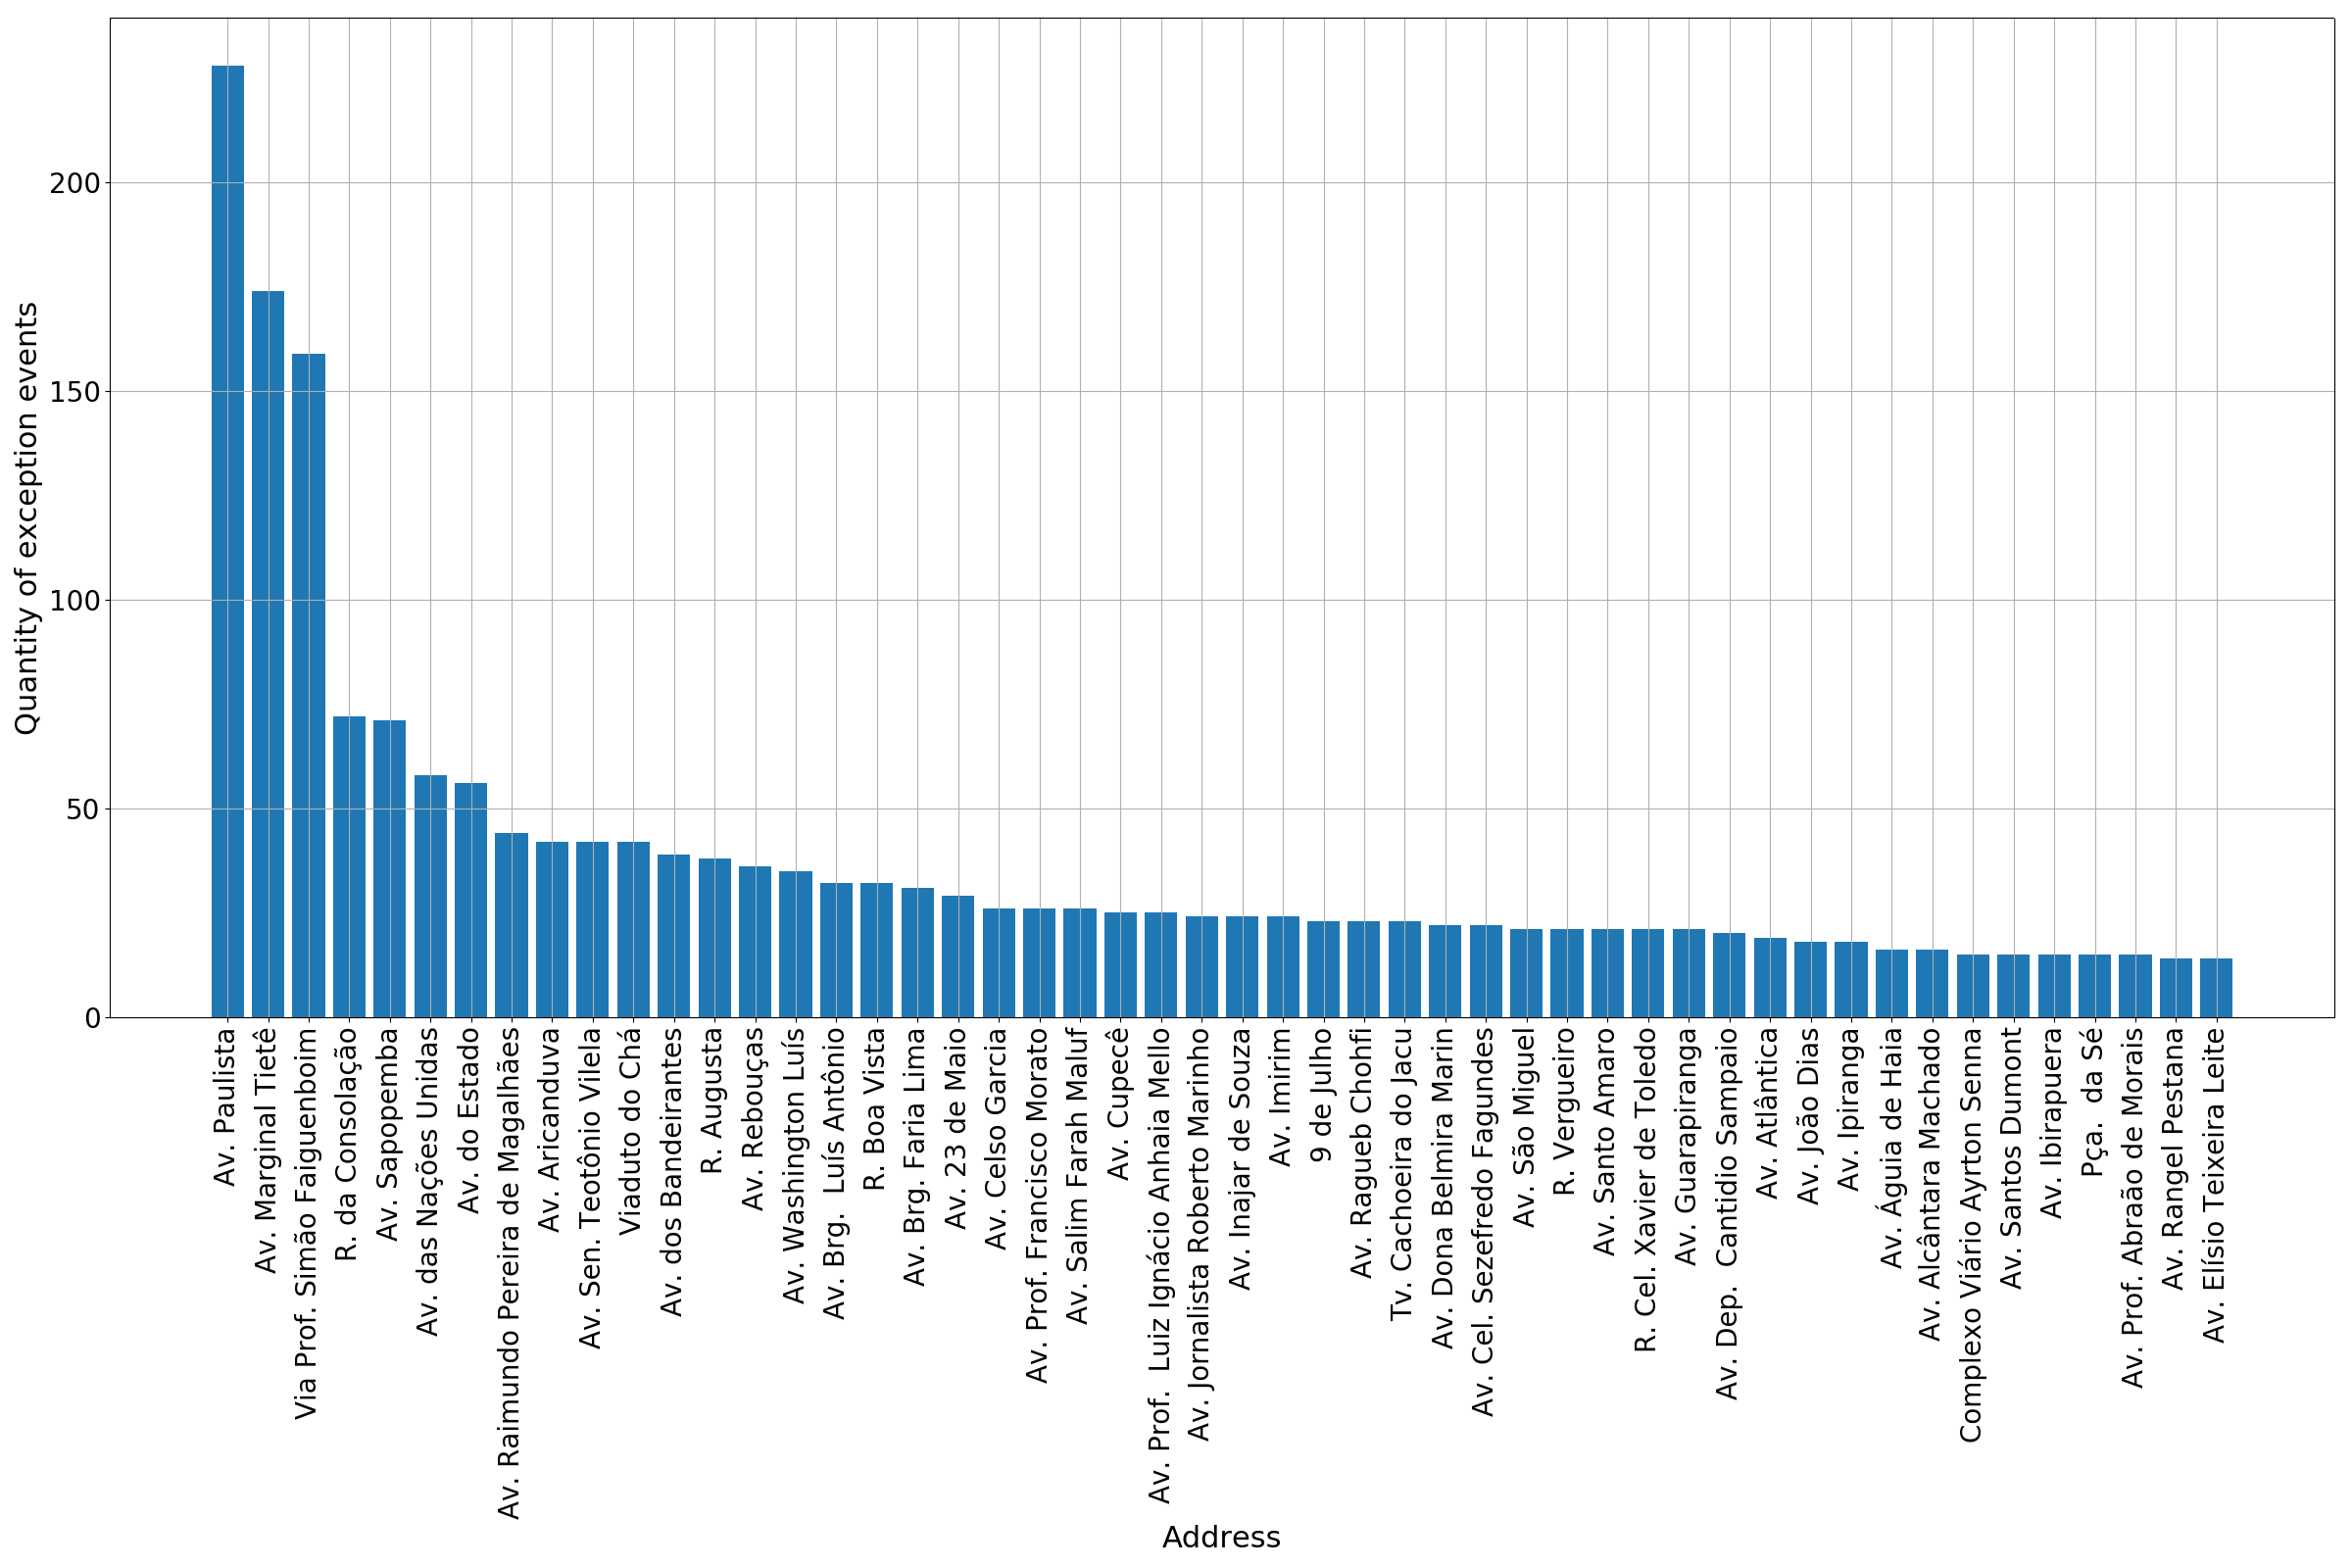
\includegraphics[width=1\linewidth]{images/address_analysis.png}
	\label{fig:address_analysis}
\end{figure}

\begin{figure}[!htb]
	\centering
 	  \caption{Distribuição dos eventos de exceção na região central de São Paulo}
		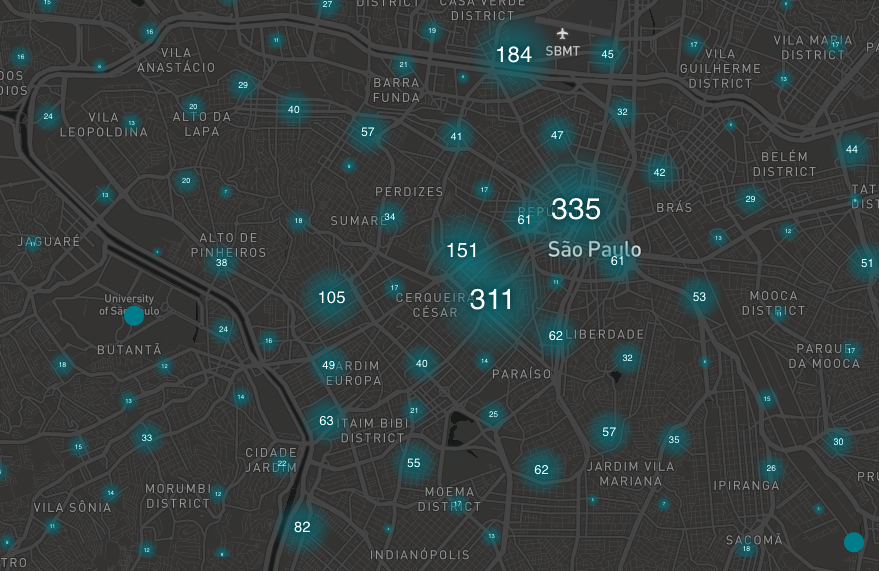
\includegraphics[width=1\linewidth]{images/exception_events_sp.png}
	\label{fig:dispersion}
\end{figure}

Consideramos que uma linha de ônibus é afetada por um evento de exceção se uma \textit{stop} estiver dentro de um raio de 1000 metros de distância do evento. Utilizando este critério, o total de 992 linhas de ônibus foram afetadas por eventos de exceção durante este período, sendo ``33389'' o código de linha de ônibus mais impactado. Essa linha específica foi impactada por 1.301 eventos de exceção. A Tab.  \ref{tab:impacted_bus_code_lines} lista as linhas de ônibus que foram impactadas por mais de 600 eventos de exceção.

\begin {table} [!htb]
\centering
\resizebox{16cm}{!}{
\begin{threeparttable}
\caption {Linhas de ônibus mais impactadas por eventos de exceção\tnote{a}}
\label {tab:impacted_bus_code_lines}
\begin {tabular} {c|c|c}
 \hline
\textbf{Código da linha} & \textbf{\# eventos de exceção} & \textbf{Letreiro} \\
    \hline
    33389 & 1301  & TERM. PINHEIROS / METRÔ TUCURUVI  \\
\hline

    33284 & 1176  & ITAIM BIBI / METRÔ SANTANA  \\
\hline

    33121 & 1023  & TERM. PRINC. ISABEL / TERM. STO. AMARO  \\
\hline

    32805 & 1006  & TERM. PRINC. ISABEL / CHÁC. SANTANA  \\
\hline

    33112 & 933   & TERM. PQ. D. PEDRO II / JD. SÃO SAVÉRIO  \\
\hline

    33111 & 857   & TERM. AMARAL GURGEL / JD. DA SAÚDE  \\
\hline

    35229 & 841   & TURISMO / CIRCULAR  \\
\hline

    33443 & 816   & ANA ROSA / METRÔ SANTANA  \\
\hline

    32897 & 805   & LUZ / TERM. A. E. CARVALHO  \\
\hline

    35072 & 767   & METRÔ BARRA FUNDA / CONEXÃO PETRÔNIO PORTELA  \\
\hline

    32772 & 759   & TERM. PRINC. ISABEL / TERM. STO. AMARO  \\
\hline

    33253 & 754   & METRÔ BELÉM / JD. BONFIGLIOLI  \\
\hline

    33391 & 748   & METRÔ JABAQUARA / METRÔ SANTANA  \\
\hline

    32813 & 746   & PÇA. DA SÉ / CHÁC. SANTANA  \\
\hline

    32829 & 746   & TERM. BANDEIRA / TERM. CAPELINHA  \\
\hline

    34048 & 719   & LGO. SÃO FRANCISCO / JD. SELMA  \\
\hline

    33486 & 715   & TERM. PQ. D. PEDRO II / TERM. SÃO MATEUS  \\
\hline

    33236 & 708   & TERM. BANDEIRA / JD. JAQUELINE  \\
\hline

    33336 & 697   & PINHEIROS / IMIRIM  \\
\hline

    32816 & 693   & TERM. PQ. D. PEDRO II / TERM. STO. AMARO  \\
\hline

    33534 & 690   & CARDOSO DE ALMEIDA / MACHADO DE ASSIS  \\
\hline

    32838 & 647   & PÇA. DA SÉ / PQ. RES. COCAIA  \\
\hline

    33398 & 639   & CID. UNIVERSITÁRIA / METRÔ SANTANA  \\
\hline

    32769 & 638   & LGO. SÃO FRANCISCO / TERM. CAPELINHA  \\
\hline

    33114 & 637   & TERM. PINHEIROS / SACOMÃ  \\
\hline

    34210 & 637   & LGO. SÃO FRANCISCO / TERM. VARGINHA  \\
\hline

    33116 & 625   & RIO PEQUENO / IPIRANGA  \\
\hline

    33126 & 614   & TERM. BANDEIRA / INOCOOP CAMPO LIMPO  \\
\hline
\end{tabular}
\begin{tablenotes}
            \item[a] Tabela completa no apêndice \ref{apendiceD}.
        \end{tablenotes}
\end{threeparttable}
}
\end{table}

\section{Considerações finais sobre a metodologia desenvolvida}

Este experimento apresenta uma nova metodologia para classificação de eventos de exceção e analisa seus respectivos impactos no sistema de transporte coletivo por ônibus da cidade de São Paulo. Com o conjunto de dados utilizados, descobrimos que o melhor algoritmo para classificar \textit{tweets} em eventos de exceção foi \textit{Multi-layer Perceptron}. Também, mostramos que é possível extrair endereços de \textit{tweets} semi-estruturados usando apenas expressões regulares. A classificação desses eventos é o primeiro passo para entender melhor como os eventos de exceção afetam a rede de transporte público.

Embora o método tenha sido validado usando perfis selecionados do Twitter escritos em português do Brasil, o mesmo pode ser generalizado para diferentes idiomas e cidades. A GTFS é um formato ubíquo para o transporte público e ferramentas como a NLTK suporta vários idiomas.

%\subsection{Future work}
%As future work, the methodology presented in this paper will be applied to the other accounts from the Corpus Twitter, described in the Section~\ref{corpusTwitter}. Besides, we will extract features from the dataset of bus movements, for each bus line affected by the exception events, also we will extract more exception events from another dataset related to reclamations made by bus users to enrich the impact analysis.

%\chapter{Proposta de pesquisa}
%\label{proposta}
%Neste capítulo, são apresentadas as seções referentes a proposta de pesquisa para a dissertação. Assim, abordaremos a formalização do problema; solução proposta; construção do conjunto de dados; exploração e visualização do conjunto de dados; identificação dos eventos de exceção; correlação dos eventos de exceção com os dados AVL da SPTrans e, por fim, o plano de trabalho.

%\section{Formalização do problema}
%\label{problemForm}

%O problema de caracterização de eventos de exceção e de seus respectivos impactos envolve a fase conhecida como \textit{feature extraction}, do ciclo iterativo do processo de \textit{feature engineering}. \textit{Feature extraction} consiste na extração de um conjunto de características ${\alpha =}$ $\lbrace {\chi_1}, {\chi_2}, ..., {\chi_n} \rbrace$ a partir de um dado de entrada $\chi$. Sendo assim, nessa proposta de pesquisa pretendemos extrair o conjunto de características (utilizando o Corpus \textit{Twitter}) ${E = }$ $\lbrace {\varepsilon_1}, {\varepsilon_2}, ..., {\varepsilon_n} \rbrace$, referente a cada evento de exceção, e o conjunto ${I_{\varepsilon_i} = }$ $\lbrace {\iota_{1\varepsilon_i}}, {\iota_{2\varepsilon_i}}, ..., {\iota_{n\varepsilon_i}} \rbrace$, contendo as características de cada impacto (utilizando o Corpus SPTrans) decorrente de um determinado evento de exceção $\varepsilon_i \in E$.

%Posto que os conjuntos \textit{E} e \textit{I} existem,  tem-se também como problema a correlação de cada evento de exceção com o seu respectivo impacto, permitindo assim uma análise histórica para identificação de padrões de causa e consequência. Tal correlação pode ser definida por uma função sobrejetora, representada formalmente em lógica de primeira ordem pela expressão:
%\begin{equation*} 
%\forall \iota \in I, \exists \varepsilon \in E (\iota = f(\varepsilon) ) 
%\end{equation*}

%Dessa forma, para todo impacto $\iota$ pertencente ao conjunto \textit{I} existe um evento de exceção $\varepsilon_i$ pertencente ao conjunto \textit{E}. 

%\section{Solução proposta}
%\label{solutionProp}

%A solução proposta pretende coletar \textit{tweets} dos \textit{profiles} contidos na tabela \ref{tab:oficialProfiles}, pré-processá-los, extrair e selecionar \textit{features} para serem utilizadas em algoritmos de classificação, obtendo dessa forma os eventos de exceção. 
%Com esses eventos de exceção pretendemos analisar a base histórica da SPTrans de dados AVL (transmitidos utilizando AVL), e identificar os possíveis impactos de cada evento de exceção. O processo de identificação dos impactos contidos na base histórica da SPTrans pode ser definido com base nas localizações extraídas dos \textit{tweets} coletados e posteriormente geolocalizadas. 

%As localizações dos \textit{tweets} podem ser extraídas usando a seguinte fórmula em expressão regular: 
%\begin{equation}
%ER = \lbrace L_1|S_1|L_2|S_2|...|L_n|S_n \rbrace \lbrace [a-zA-Z \backslash s]+ \rbrace
%\end{equation}
%Tal expressão regular é dividida em dois conjuntos, no primeiro ($\lbrace L_1|S_1|L_2|S_2|...|L_n\\|S_n \rbrace$), os logradouros (L) e siglas (S) contidas na tabela \ref{tab:logradouros} (no apêndice \ref{apendiceB}) são concatenadas, especificando um filtro para identificar cadeias de caracteres iniciadas com um logradouro ou sigla. No segundo conjunto ($\lbrace [a-zA-Z \backslash s]+ \rbrace$), o filtro especificado identifica as palavras seguintes aos logradouros e siglas.

%Em resumo, propomos solucionar o problema de caracterização dos eventos de exceção e de seus respectivos impactos seguindo os seguintes passos: (I) coleta de \textit{tweets} de órgãos responsáveis por notificar eventos de exceção; (II) identificação dos \textit{tweets} relacionados a eventos de exceção; (III) extração e geolocalização dos endereços dos eventos de exceção e (IV) análise e correlação com os dados AVL.

%\subsection{Algoritmos de Aprendizado de Máquina}

%Após a extração e seleção de \textit{features}, planejamos classificar manualmente 30\% dos \textit{tweets} com base em suas respectivas \textit{features}, utilizando-os como conjunto de teste. Posteriormente, pretendemos analisar os algoritmos de aprendizado de máquina elencados pela revisão sistemática em \ref{iaClassification} para escolhermos dentre eles o com maior acurácia para identificar eventos de exceção, por meio de classificação.

%\section{Plano de trabalho}
%\label{workPlan}

%Nesta seção, são apresentados o cronograma (tabela \ref{tab:schedule}) e as atividades realizadas e planejadas para o desenvolvimento do projeto referente a proposta de pesquisa, enumeradas a seguir:

%\begin{enumerate}
%\item Revisão Bibliográfica.
%\begin{enumerate}
%\item Revisão Sistemática sobre estudos de caso utilizando \textit{tweets} na caracterização de problemas urbanos e relacionados ao transporte público.
%\end{enumerate}
%\item Desenvolvimento de protótipo.
%\begin{enumerate}
%\item Serviço para coleta, processamento e armazenamento de \textit{tweets} dos \textit{profiles} selecionados contidos na tabela \ref{tab:oficialProfiles}.
%\item Extração e geolocalização dos endereços contidos nos \textit{tweets}.
%\item Implementação de \textit{scripts} para extração, transformação e armazenamento dos dados AVL da SPTrans.
%\item Implementação de \textit{scripts} para extração, transformação e armazenamento dos dados da GTFS da SPTrans.
%\item Criação de especificações de ingestão de dados para os dados AVL da SPTrans e dos \textit{tweets} dos \textit{profiles} selecionados contidos na tabela \ref{tab:oficialProfiles} para o banco de dados de séries temporais \textit{Druid}\footnote{\label{druidIo}\url{http://druid.io}. Acesso em Outubro, 29 de 2017.}.
%\item Integração da ferramenta \textit{Superset}\footnote{\label{superset}\url{http://superset.apache.org}. Acesso em Outubro, 29 de 2017.} com o \textit{Druid}\footref{druidIo} para exploração e visualização dos dados AVL da SPTrans e dos \textit{tweets} dos \textit{profiles} selecionados contidos na tabela \ref{tab:oficialProfiles}.
%\item Implementação de \textit{scripts} para automação dos processos de ingestão de dados e \textit{deploy} e monitoramento dos serviços do \textit{Druid}\footref{druidIo} e Superset\footref{superset}.
%\item Configuração do ambiente em nuvem para execução do \textit{Druid}\footref{druidIo} e \textit{Superset}\footref{superset}.

%\end{enumerate}
%\item Construção do conjunto de dados.
%\begin{enumerate}
%\item Obtenção dos dados AVL de janeiro a dezembro de 2016 e de janeiro a setembro de 2017, de todas as linhas de ônibus de São Paulo.
%\item Obtenção da base de dados dos últimos cinco anos das reclamações relacionadas a SPTrans, realizadas na Central de Atendimento ao Cidadão (156) da Prefeitura de São Paulo.
%\item Obtenção de um conjunto de \textit{tweets} dos \textit{profiles} selecionados contidos na tabela \ref{tab:oficialProfiles}.
%\end{enumerate}
%\item Implementação da solução proposta.
%\begin{enumerate}
%\item Identificação dos eventos de exceção (pré-processamento, \textit{feature extraction} e \textit{feature selection} dos \textit{tweets} coletados).
%\item Estudo dos algoritmos de classificação e implementação de um artefato de \textit{software} para classificação dos \textit{tweets} de acordo com seus respectivos eventos de exceção.
%\item Correlação dos eventos de exceção com os dados AVL da SPTrans.
%\end{enumerate}
%\item Avaliação dos resultados parciais obtidos durante e após o desenvolvimento da solução proposta.
%\item Escrita de artigo para submissão em periódicos ou eventos da área.
%\item Escrita da dissertação.
%\end{enumerate}

%\begin{table}[!htb]
%  \centering
%  \caption{Cronograma de atividades}
%  \resizebox{\textwidth}{!}{%
%    \begin{tabular}{cccccccccccccccccccc} \hline
%    \multicolumn{2}{c}{Atividade } & \multicolumn{12}{c}{2017}                                                                     & \multicolumn{6}{c}{2018} \\ 
%    Número & Descrição & 1     & 2     & 3     & 4     & 5     & 6     & 7     & 8     & 9     & 10    & 11    & 12    & 1     & 2     & 3     & 4     & 5     & 6 \\ \hline
%    1     & Revisão bibliográfica & X     & X     & X     & X     & X     & X     &       &       &       &       &       &       &       &       &       &       &       &  \\
%    2     & Desenvolvimento de protótipo &       &       & X     & X     & X     & X     &       &       &       &       &       &       &       &       &       &       &       &  \\
%    3     & Construção do conjunto de dados &       &       &       &       &       &       & X     & X     & X     & X     & X     &       &       &       &       &       &       &  \\
%    4     & Implementação da solução proposta &       &       &       &       &       &       &     &      &      &      &      & X     &   X    &  X     &   X    &  X   &   X   &  \\
%    5     & Avaliação dos resultados &       &       &       &       &       &       &       &       &       &      &     &      &   X    &       &   X    &       &   X    &  \\
%    6    & Escrita de artigo &       &       &       &       &       &       &       &       &       &       &      &       &       &   X    &   X    &       &       &  \\ 
%    7     & Escrita da dissertação &       &       & X     & X     & X     & X     & X     & X     & X     & X     & X     & X     & X     & X     & X     & X     & X     & X \\
%    \hline
%    \end{tabular}%
%    }
%  \label{tab:schedule}%
% \source{Felipe Cordeiro Alves Dias, 2017}
%\end{table}%

\chapter{Correlação dos eventos de exceção com os dados AVL da SPTrans}
\label{dataCorr}
\todo[inline]{Escrever Correlação dos eventos de exceção com os dados AVL da SPTrans}

Dado que os eventos de exceção podem ser identificados utilizando \textit{tweets} dos \textit{profiles} contidos na tabela \ref{tab:oficialProfiles}, há também a possibilidade de caracterizarmos seus respectivos impactos analisando a base histórica dos dados AVL da SPTrans, especificamente os dados referentes a \textit{timestamp}, latitude, longitude, \textit{bus\_id} e \textit{trip\_id}. Dito isso, inicialmente pretendemos caracterizar os impactos em:

\begin{itemize}
\item Atraso médio induzido nas viagens.
\item Ônibus frequentemente afetados por eventos de exceção.
\item Ônibus frequentemente afetados por determinado evento de exceção.
\item Padrão de ocorrência dos eventos de exceção no espaço-tempo (localizações e \textit{timestamps}).
\item Quantidade e viagens afetadas.
\item Quantidade e regiões da cidade de São Paulo afetadas.
\item Viagens frequentemente afetadas por eventos de exceção.
\item Viagens frequentemente afetadas por determinado evento de exceção.
\end{itemize}

\begin{figure}[!htb]
	\centering
 	  \caption{Matriz de confusão relacionada a classificação dos \textit{tweets} em eventos de exceção por meio do algoritmo \textit{Multi-layer Perceptron}}
		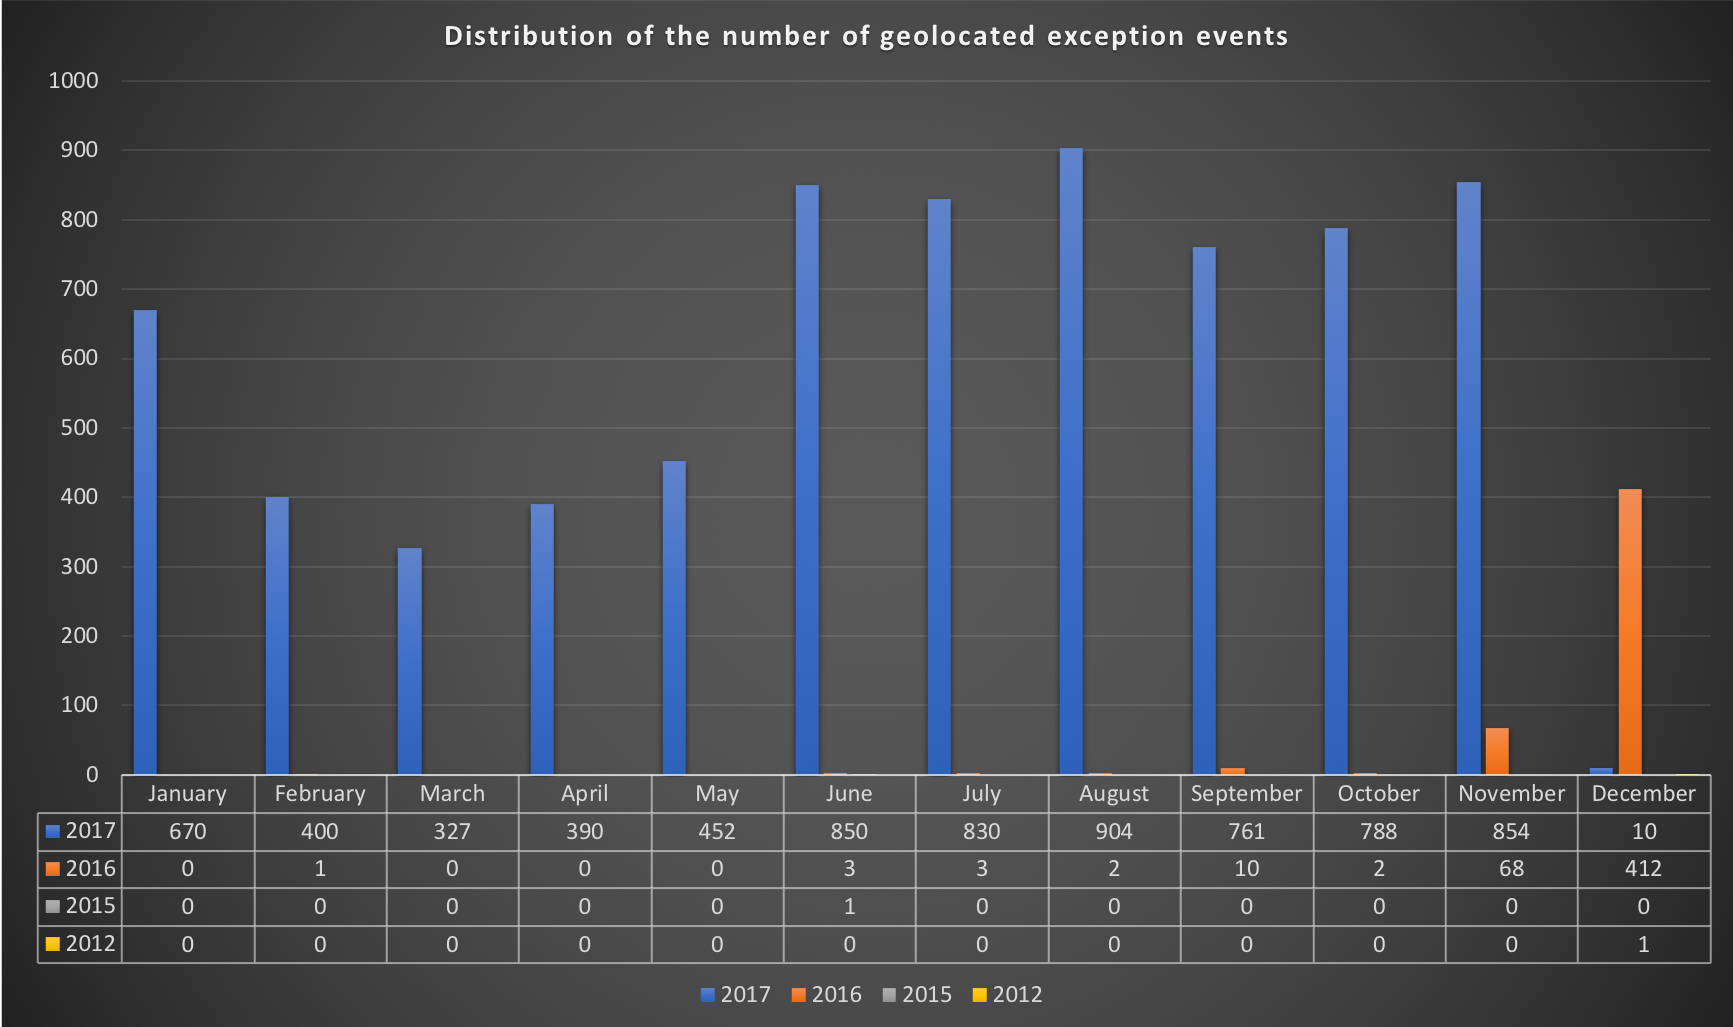
\includegraphics[width=1\linewidth]{images/geolocated_exception_events_distribution.png}
	\label{fig:geolocated_exception_events_distribution}
\end{figure}

\chapter{Conclusão}
\label{conclusion}

Neste capítulo, são apresentadas as contribuições e resultados esperados com o projeto de pesquisa, as limitações a ameaças à validade do estudo. 

\section{Contribuições}

A principal contribuição deste projeto é propor uma solução para o problema de caracterização de eventos de exceção e de seus respectivos impactos no sistema de transporte público por ônibus da cidade de São Paulo, por meio de \textit{tweets} e de dados históricos dos módulos AVL do SIM. Além disso, a solução proposta visa disponibilizar os conjuntos de dados que foram construídos e uma plataforma para que esses dados possam ser visualizados e explorados, de forma a contribuir com projetos e pesquisas futuras correlatas.

Em relação a publicações científicas, serão submetidos artigos com os resultados obtidos para veículos de disseminação de conhecimento científico nas áreas de: Análise de Redes Sociais, Sistemas de Transporte Inteligentes, Cidades Inteligentes.

\section{Trabalhos publicados}
\todo[inline]{Escrever trabalhos publicados}

\section{Trabalhos futuros}
\todo[inline]{Escrever trabalhos futuros}
As principais limitações deste projeto estão relacionadas ao processamento de \textit{tweets} em português brasileiro e oriundos das contas selecionadas e referenciadas na tabela \ref{tab:oficialProfiles}, o que pode tornar a solução não generalista. Dentre os riscos, apesar das análises preliminares realizadas para extração de endereços dos conteúdos dos \textit{tweets} por meio de Expressão Regular, é possível que sejam encontrados novos desafios que inviabilizem o uso dessa técnica.

\section*{Acknowledgment}
This research is part of the INCT of the Future Internet for Smart Cities funded by CNPq, proc. 465446/2014-0, CAPES proc.88887.136422/2017-00, and FAPESP, proc. 2014/50937-1.

% ----------------------------------------------------------
% ELEMENTOS PÓS-TEXTUAIS
% ----------------------------------------------------------
\postextual
% ----------------------------------------------------------

% ----------------------------------------------------------
% Referências bibliográficas
% ----------------------------------------------------------
\listoftodos[Notes]
\bibliography{referencias}

% ----------------------------------------------------------
% Glossário
% ----------------------------------------------------------
%
% Consulte o manual da classe abntex2 para orientações sobre o glossário.
%
%\glossary

% ----------------------------------------------------------
% Apêndices
% ----------------------------------------------------------

% ---
% Inicia os apêndices
% ---
\begin{apendicesenv}

% Imprime uma página indicando o início dos apêndices
\partapendices
\chapter{Exemplos de \textit{tweets}}
\label{apendiceA}

\begin{lstlisting}[language=json,title=Exemplos de \textit{tweets} dos \textit{profiles} selecionados citados na tabela \ref{tab:oficialProfiles}, label=tweetsSample]
{
    "tweet_id" : 895060642952077314,
    "tweet_account": "BombeirosPMESP",
    "text" : "19h58 Colisão de Carro x Caminhão, Estrada Sta Isabel, 5950 Itaquaquecetuba. 2 Vítimas, 1 Vtr. Aguardando maiores informes"
}
{
    "tweet_id" : 894707930217447427,
    "tweet_account": "CETSP_",
    "text" : "Referente manifestação Rua Augusta, pista liberada.#ZC"
}
{
    "tweet_id" : 894147793060716544,
    "tweet_account": "CPTM_oficial",
    "text" : "#L11 Hoje, das 8h à meia-noite, circulação interrompida entre Luz e Brás. P/ seguir viagem, use a L7-Rubi q prestará serviço até a Est. Brás"
}
{
    "tweet_id" : 895054721026838530,
    "tweet_account": "governosp",
    "text" : "@SANROGE Lamentamos o ocorrido, Rogerio. Estamos trabalhando continuamente para melhorar a segurança na região. Entre maio e junho, [+] [1]"
}
{
    "tweet_id" : 895000711284621312,
    "tweet_account": "metrosp_oficial",
    "text" : "08/08/2017 16:16: #metrosp : Linha 5-Lilás: Velocidade Reduzida. Mais informações em https://t.co/CaeqD26iJR"
}
{
    "tweet_id" : 884039273493803008,
    "tweet_account": "PMESP",
    "text" : "AGORA: Desfile Cívico-Militar de 9 de Julho no Obelisco - Ibirapuera SP, transmissão ao vivo na página oficial Facebook da Polícia Militar.",
    "dateTime" : "2017-07-09 10:19:22"
}
{
    "tweet_id" : 887315002117500932,
    "tweet_account": "Policia_Civil",
    "text" : "Polícia Civil realiza operação para combater a prática do Jogo conhecido como "Baleia Azul"... https://t.co/kh2HW6UZvT",
}
{
    "tweet_id" : 895004079910518788,
    "tweet_account": "saopaulo_agora",
    "text" : "#ItaimPaulista Incêndio na Rua Mateus Barbosa de Resende nº 235. Defesa Civil Regional acionada para o local. (CCOI) #spagora"
}
{
    "tweet_id" : 894694704989732864,
    "tweet_account": "smtpsp_",
    "text" : "A @sptrans_ irá modificar 14 linhas na Zona Leste para obras no Monotrilho Saiba mais: https://t.co/fCA0T7WCSY"
}
{
    "tweet_id" : 902953598857949184,
    "tweet_account": "SPCEDEC",
    "text" : "30-08-2017 - Acidente com produto perigoso em  com 36 , deixa 21 vítimas feridas e 02 ."
}
{
    "tweet_id" : 895065137484320769,
    "tweet_account": "sptrans_",
    "text" : "Obras do Monotrilho desviam itinerários de 14 linhas que atendem a Av. Sapopemba entre 5 e 11/08, das 23h às 5h: https://t.co/jH4LFgrSKZ"
}
{
    "tweet_id : 895042604068458497,
    "tweet_account": "TurismoSaoPaulo",
    "text" : "Veganos, vegetarianos e simpatizantes: vem aí o Vegan Club, em 12/08, no Centro de SP! #crueltyfree #veganfood... https://t.co/7f7ggr4vn4"
}
\end{lstlisting}

\clearpage

\chapter{Logradouros utilizados}
\label{apendiceB}

\begin{longtable}{c|c}
\caption{Tabela de logradouros com abreviaturas}
\label{tab:logradouros}\\

\hline \multicolumn{1}{c |}{\textbf{Abreviatura}} & \multicolumn{1}{c}{\textbf{Logradouro}} \\ \hline 
\endfirsthead

\multicolumn{2}{c}%
{{\bfseries \tablename\ \thetable{} -- continuação da página anterior}} \\
\hline \multicolumn{1}{c |}{\textbf{Abreviatura}} & \multicolumn{1}{c}{\textbf{Logradouro}}  \\ \hline 
\endhead

\hline \multicolumn{2}{r}{{Continua na próxima página}} \\
\endfoot

\hline \hline
\endlastfoot

\hline
ACAMP & Acampamento \\
\hline
AC & Acesso \\
\hline
AD & Adro \\
\hline
ERA & Aeroporto \\
\hline
AL & Alameda \\
\hline
AT & Alto \\
\hline
A & Area \\
\hline
AE & Area especial \\
\hline
ART & Arteria \\
\hline
ATL & Atalho \\
\hline
AV & Avenida \\
\hline
AV-CONT & Avenida contorno \\
\hline
BX & Baixa \\
\hline
BLO & Balao \\
\hline
BAL & Balneario \\
\hline
BC & Beco \\
\hline
BELV & Belvedere \\
\hline
BL & Bloco \\
\hline
BSQ & Bosque \\
\hline
BVD & Boulevard \\
\hline
BCO & Buraco \\
\hline
C & Cais \\
\hline
CALC & Calcada \\
\hline
CAM & Caminho \\
\hline
CPO & Campo \\
\hline
CAN & Canal \\
\hline
CHAP & Chacara \\
\hline
CHAP & Chapadao \\
\hline
CIRC & Circular \\
\hline
COL & Colonia \\
\hline
CMP-VR & Complexo viario \\
\hline
COND & Condominio \\
\hline
CJ & Conjunto \\
\hline
COR & Corredor \\
\hline
CRG & Corrego \\
\hline
DSC & Descida \\
\hline
DSV & Desvio \\
\hline
DT & Distrito \\
\hline
EVD & Elevada \\
\hline
ENT-PART & Entrada particular \\
\hline
EQ & Entre quadra \\
\hline
ESC & Escada \\
\hline
ESP & Esplanada \\
\hline
ETC & Estacao \\
\hline
ESTC & Estacionamento \\
\hline
ETD & Estadio \\
\hline
ETN & Estancia \\
\hline
EST & Estrada \\
\hline
EST-MUN & Estrada municipal \\
\hline
FAV & Favela \\
\hline
FAZ & Fazenda \\
\hline
FRA & Feira \\
\hline
FER & Ferrovia \\
\hline
FNT & Fonte \\
\hline
FTE & Forte \\
\hline
GAL & Galeria \\
\hline
GJA & Granja \\
\hline
HAB & Habitacional \\
\hline
IA & Ilha \\
\hline
JD & Jardim \\
\hline
JDE & Jardinete \\
\hline
LD & Ladeira \\
\hline
LG & Lago \\
\hline
LGA & Lagoa \\
\hline
LRG & Largo \\
\hline
LOT & Loteamento \\
\hline
MNA & Marina \\
\hline
MOD & Modulo \\
\hline
TEM & Monte \\
\hline
MRO & Morro \\
\hline
NUC & Nucleo \\
\hline
PDA & Parada \\
\hline
PDO & Paradouro \\
\hline
PAR & Paralela \\
\hline
PRQ & Parque \\
\hline
PSG & Passagem \\
\hline
PSC-SUB & Passagem subterranea \\
\hline
PSA & Passarela \\
\hline
PAS & Passeio \\
\hline
PAT & Patio \\
\hline
PNT & Ponta \\
\hline
PTE & Ponte \\
\hline
PTO & Porto \\
\hline
PC & Praca \\
\hline
PC-ESP & Praça de esportes \\
\hline
PR & Praia \\
\hline
PRL & Prolongamento \\
\hline
Q & Quadra \\
\hline
QTA & Quinta \\
\hline
QTAS & Quinta \\
\hline
RAM & Rama \\
\hline
RMP & Rampa \\
\hline
REC & Recanto \\
\hline
RES & Residencial \\
\hline
RET & Reta \\
\hline
RER & Retiro \\
\hline
RTN & Retorno \\
\hline
ROD-AN & RodoAnel \\
\hline
ROD & Rodovia \\
\hline
RTT & Rotatoria \\
\hline
ROT & Rotula \\
\hline
R & Rua \\
\hline
R-LIG & Rua de ligação \\
\hline
R-PED & Rua de pedrestre \\
\hline
SRV & Servidao \\
\hline
ST & Setor \\
\hline
SIT & Sitio \\
\hline
SUB & Subida \\
\hline
TER & Terminal \\
\hline
TV & Travessa \\
\hline
TV-PART & Travessa particular \\
\hline
TRV & Trecho \\
\hline
TRV & Trevo \\
\hline
TCH & Trincheira \\
\hline
TUN & Tunel \\
\hline
UNID & Unidade \\
\hline
VAL & Vala \\
\hline
VLE & Vale \\
\hline
VRTE & Variante \\
\hline
VER & Vereda \\
\hline
V & Via \\
\hline
V-AC & Via de acesso \\
\hline
V-PED & Via de pedestre \\
\hline
V-EVD & Via elevado \\
\hline
V-EXP & Via expressa \\
\hline
VD & Viaduto \\
\hline
VLA & Viela \\
\hline
VL & Vila \\
\hline
ZIG-ZAG & Zigue-zague \\

\end{longtable}

\center{\textbf{Fonte:}} MS/SAS/DRAC/CGSI - Coordenação Geral dos Sistemas de Informação (adaptada)\footnote{\url{http://www.pmf.sc.gov.br/arquivos/arquivos/pdf/04_01_2010_10.27.25.2b615e6755138defe1bdb00f1c86031f.PDF}. Acesso em Outubro, 29 de 2017.}

\clearpage


%-------------------------------------------------------------------------
% Comentário adicional do PPgSI - Informações sobre ``apêndice''
%
% Para todos os captions/(títulos) (de seções, subseções, tabelas, 
% ilustrações, etc.):
%     - em maiúscula apenas a primeira letra da sentença (do título), 
%       exceto nomes próprios, geográficos, institucionais ou Programas ou
%       Projetos ou siglas, os quais podem ter letras em maiúscula também.
%
% Todas  as tabelas, ilustrações (figuras, quadros, gráficos etc. ), 
% anexos, apêndices devem obrigatoriamente ser citados no texto.
%      - a citação deve vir sempre antes da primeira vez em que a tabela, 
%        ilustração etc., aparecer pela primeira vez.
%
%-------------------------------------------------------------------------
\chapter{Detalhamento dos campos da GTFS}
\label{apendiceC}


%---------------------------------------------------------------------
% INDICE REMISSIVO
%---------------------------------------------------------------------
%%%%%MF\phantompart
%%%%%MF\printindex
%---------------------------------------------------------------------

\begin{table}[!htb]
\centering
  \caption{Detalhamento dos campos do arquivo \textit{agency.txt} da GTFS}
      \label{tab:gtfsAgency}
\begin{tabular}{>{\centering\arraybackslash}m{3.5cm} | >{\centering}m{3cm} | >{\centering\arraybackslash}m{8cm}}
\hline
\textbf{Nome do campo} & \textbf{Condicional} & \textbf{Descrição} \\
\hline
\textit{agency\_id} & Opcional & Identifica uma agência de transporte público. Um \textit{feed} de transporte público pode representar dados de mais de uma agência. Este campo é opcional para \textit{feeds} de transporte público que contenham somente dados de uma única agência. \\
\hline
\textit{agency\_name} & Obrigatório & Contém o nome completo da agência de transporte público. \\
\hline
\textit{agency\_url} & Obrigatório & Contém o \textit{URL} da agência de transporte público. \\
\hline
\textit{agency\_timezone} & Obrigatório & Contém o fuso horário de onde a agência de transporte público está localizada. \\
\hline
\textit{agency\_lang} & Opcional & Contém um código \textit{ISO 639-1} de duas letras para o idioma principal usado por essa agência de transporte público. \\
\hline
\textit{agency\_phone} & Opcional & Contém um único número de telefone da agência especificada. \\
\hline
\textit{agency\_fare\_url} & Opcional & Especifica o \textit{URL} de uma página da \textit{Web} que permite que um passageiro compre passagens ou outros instrumentos de tarifas dessa agência \textit{on-line}. \\
\hline
\end{tabular}
\end{table}
\vspace{-\baselineskip}
\center{\textbf{Fonte:}} Google Transit (adaptada)\footnote{\label{gtfsFields}\url{https://developers.google.com/transit}. Acesso em Outubro, 29 de 2017.}

\clearpage

\begin{longtable}[!htb]{>{\centering\arraybackslash}m{3.8cm} | >{\centering}m{2.5cm} | >{\centering\arraybackslash}m{8.5cm}}
  \caption{Detalhamento dos campos do arquivo \textit{stops.txt} da GTFS}
      \label{tab:gtfsStops} \\

\hline \multicolumn{1}{>{\centering\arraybackslash}m{3.8cm} |}{\textbf{Nome do campo}} & \multicolumn{1}{>{\centering}m{2.5cm} | }{\textbf{Condicional}} & \multicolumn{1}{>{\centering\arraybackslash}m{8.5cm}}{\textbf{Descrição}}\\ \hline 
\endfirsthead

\multicolumn{3}{c}%
{{\bfseries \tablename\ \thetable{} -- continuação da página anterior}} \\
\hline \multicolumn{1}{>{\centering\arraybackslash}m{3.8cm} |}{\textbf{Nome do campo}} & \multicolumn{1}{>{\centering}m{2.5cm} |}{\textbf{Condicional}} & \multicolumn{1}{>{\centering\arraybackslash}m{8.5cm}}{\textbf{Descrição}}  \\ \hline 
\endhead

\hline \multicolumn{3}{c}{{Continua na próxima página}} \\
\endfoot

\hline \hline
\endlastfoot     
      
\hline
\textit{stop\_id} & Obrigatório & Contém um ID que identifica uma parada ou uma estação. Diversos trajetos podem usar a mesma parada. \\
\hline
\textit{stop\_code} & Opcional & Contém um pequeno texto ou um número que identifica a parada para os passageiros. Os códigos das paradas são usados muitas vezes em sistemas de informações sobre transporte público por telefone ou impressos em sinalizações nas paradas para que os passageiros possam obter informações sobre o horário das paradas com mais facilidade ou sobre chegadas de uma parada específica em tempo real. O campo \textit{stop\_code} só deve ser usado para códigos de parada exibidos aos passageiros. Para os códigos internos, use \textit{stop\_id}. Este campo deve ser deixado em branco para as paradas que não têm um código. \\
\hline
\textit{stop\_name} & Obrigatório & Contém o nome de uma parada ou estação. Use um nome compreensível para as pessoas locais e linguagem turística. \\
\hline
\textit{stop\_desc} & Opcional & Contém uma descrição de uma parada. Forneça informações úteis e de qualidade. Não basta repetir o nome da parada. \\
\hline
\textit{stop\_lat} & Obrigatório & Contém a latitude de uma parada ou estação. O valor do campo deve ser uma latitude WGS 84 válida. \\
\hline
\textit{stop\_lon} & Obrigatório & Contém a longitude de uma parada ou estação. O valor do campo deve ser uma latitude WGS 84 válida entre -180 e 180. \\
\hline
\textit{zone\_id} & Opcional & Define a zona tarifária do ID de uma parada. Os IDs de zonas são obrigatórios para fornecer informações sobre tarifas usando \textit{fare\_rules.txt}. Se esse ID de parada representa uma estação, o ID de zona é ignorado. \\
\hline
\textit{stop\_url} & Opcional & Contém o URL de uma página da Web sobre uma parada específica. Ele deve ser diferente dos campos \textit{agency\_url} e \textit{route\_url}. \\
\hline
\textit{location\_type} & Opcional & Identifica se este ID de parada representa uma parada ou uma estação. Se nenhum tipo de local for especificado ou se o campo \textit{location\_type} estiver em branco, os IDs de parada serão tratados como paradas. As estações podem ter propriedades diferentes das paradas quando são representadas em um mapa ou usadas em planejamento de viagens. O campo de tipo de local pode ter os seguintes valores: 0 ou em branco (para parada) e 1 (estação). \\
\hline
\textit{parent\_station} & Opcional & Para paradas que estejam fisicamente localizadas dentro de estações, o campo \textit{parent\_station} identifica a estação associada à parada. Para usar este campo, o arquivo \textit{stops.txt} também deve conter uma linha em que esse ID de parada tenha o tipo de localização=1. \\
\hline
\textit{stop\_timezone} & Opcional & Contém o fuso horário em que a parada ou estação está localizada. Se omitido, assume-se que a parada está localizada no fuso horário especificado por \textit{agency\_timezone} no arquivo \textit{agency.txt}.
Quando uma parada tem uma estação principal, considera-se que a parada esteja no fuso horário especificado pelo valor \textit{stop\_timezone} da estação principal. Se uma parada específica possui um valor \textit{parent\_station}, qualquer valor \textit{stop\_timezone} especificado para essa parada deve ser ignorado. Mesmo que os valores de \textit{stop\_timezone} sejam fornecidos no arquivo \textit{stops.txt}, os horários em \textit{stop\_times.txt} devem continuar a ser especificados como horários desde a meia-noie no fuso horário especificado por \textit{agency\_timezone} em \textit{agency.txt}. Isso garante que os valores de tempo em uma viagem sempre aumentam durante uma viagem, independentemente dos fusos horários pelos quais uma viagem passa. \\
\hline
\textit{wheelchair\_boarding} & Opcional & Identifica se é possível o embarque de passageiros em cadeira de rodas na parada ou estação especificada. O campo pode ter os seguintes valores:
0 (ou vazio) - indica que não há informações sobre acessibilidade para a parada; 1 - indica que, pelo menos, alguns veículos nesta parada possibilitam o embarque de passageiros em cadeira de rodas; 2 - o embarque de pessoas em cadeiras de roda não é possível nesta parada. Quando uma parada faz parte de um complexo de estações maiores, como indicado por uma para com um valor \textit{parent\_station}, o campo \textit{wheelchair\_boarding} da parada possui a seguinte semântica adicional:
0 (ou vazio) - a parada herdará o valor para \textit{wheelchair\_boarding} da estação principal, se especificado; 1 - existem vias de acesso na parte externa da estação para a parada/plataforma específic; 2 - não há vias de acesso na parte externa da estação para a parada/plataforma específica \\
\end{longtable}
\vspace{-\baselineskip}
\center{\textbf{Fonte:}} Google Transit (adaptada)\footref{gtfsFields} 

\newpage

\begin{longtable}[!htb]{>{\centering\arraybackslash}m{3.8cm} | >{\centering}m{2.5cm} | >{\centering\arraybackslash}m{8.5cm}}
  \caption{Detalhamento dos campos do arquivo \textit{routes.txt} da GTFS}
      \label{tab:gtfsRoutes} \\

\hline \multicolumn{1}{>{\centering\arraybackslash}m{3.8cm} |}{\textbf{Nome do campo}} & \multicolumn{1}{>{\centering}m{2.5cm} | }{\textbf{Condicional}} & \multicolumn{1}{>{\centering\arraybackslash}m{8.5cm}}{\textbf{Descrição}}\\ \hline 
\endfirsthead

\multicolumn{3}{c}%
{{\bfseries \tablename\ \thetable{} -- continuação da página anterior}} \\
\hline \multicolumn{1}{>{\centering\arraybackslash}m{3.8cm} |}{\textbf{Nome do campo}} & \multicolumn{1}{>{\centering}m{2.5cm} |}{\textbf{Condicional}} & \multicolumn{1}{>{\centering\arraybackslash}m{8.5cm}}{\textbf{Descrição}}  \\ \hline 
\endhead

\hline \multicolumn{3}{c}{{Continua na próxima página}} \\
\endfoot

\hline \hline
\endlastfoot  

\hline
\textit{route\_id} & Obrigatório & Contém um ID que identifica um trajeto. \\
\hline
\textit{agency\_id} & Opcional & Define uma agência para o trajeto especificado. Este valor é indicado no arquivo \textit{agency.txt}. Campo destinado para quando for fornecido dados para trajetos de mais de uma agência. \\
\hline
\textit{route\_short\_name} & Obrigatório & Contém o nome abreviado de um trajeto. Geralmente, será um identificador pequeno e abstrato, como, por exemplo "32", "100X" ou "Verde", que os passageiros usam para identificar um trajeto, mas que não fornece nenhuma identificação de quais lugares são atendidos pelo trajeto. Se o trajeto não tem um nome abreviado, especifique um \textit{route\_long\_name} e use uma sequência vazia como o valor deste campo. \\
\hline
\textit{route\_long\_name} & Obrigatório & Contém o nome completo de um trajeto. Em geral, esse nome é mais descritivo que \textit{route\_short\_name} e incluirá o destino ou a parada do trajeto. Se o trajeto não tem um nome completo, especifique um \textit{route\_short\_name} e use uma sequência vazia como o valor deste campo. \\
\hline
\textit{route\_desc} & Opcional & Contém uma descrição de um trajeto. Não basta repetir o nome do trajeto. \\
\hline
\textit{route\_type} & Obrigatório & Descreve o tipo de transporte usado em um trajeto. Os valores válidos deste campo são:
0 - Bonde, ônibus elétrico, veículo leve sobre trilhos; 1 - Metrô, trem subterrâneo; 2 - Via férrea;  3 - Ônibus; 4 - Balsa; 5 - Teleférico; 6 - Gôndola, teleférico suspenso; 7 - Funicular. \\
\hline
\textit{route\_url} & Opcional & Contém o URL de uma página da Web sobre esse trajeto específico. Ele deve ser diferente de \textit{agency\_url}.\\
\hline
\textit{route\_color} & Opcional & Define uma cor que corresponda ao trajeto. A cor deve ser informada como um número hexadecimal de seis caracteres. Se nenhuma cor é especificada, a cor padrão de trajetos é branca (FFFFFF). A diferença de cores entre \textit{route\_color} e \textit{route\_text\_color} deve fornecer contraste suficiente quando visualizado em uma tela em preto e branco. \\
\hline
\textit{route\_text\_color} & Opcional & Usado para especificar uma cor legível para usar em desenho de texto contra um plano de fundo de \textit{route\_color}. \\
\end{longtable}
\vspace{-\baselineskip}
\center{\textbf{Fonte:}} Google Transit (adaptada)\footref{gtfsFields}

\newpage

\begin{longtable}[!htb]{>{\centering\arraybackslash}m{4cm} | >{\centering}m{2.5cm} | >{\centering\arraybackslash}m{8.5cm}}
  \caption{Detalhamento dos campos do arquivo \textit{trips.txt} da GTFS}
      \label{tab:gtfsTrips} \\

\hline \multicolumn{1}{>{\centering\arraybackslash}m{4cm} |}{\textbf{Nome do campo}} & \multicolumn{1}{>{\centering}m{2.5cm} | }{\textbf{Condicional}} & \multicolumn{1}{>{\centering\arraybackslash}m{8.5cm}}{\textbf{Descrição}}\\ \hline 
\endfirsthead

\multicolumn{3}{c}%
{{\bfseries \tablename\ \thetable{} -- continuação da página anterior}} \\
\hline \multicolumn{1}{>{\centering\arraybackslash}m{4cm} |}{\textbf{Nome do campo}} & \multicolumn{1}{>{\centering}m{2.5cm} |}{\textbf{Condicional}} & \multicolumn{1}{>{\centering\arraybackslash}m{8.5cm}}{\textbf{Descrição}}  \\ \hline 
\endhead

\hline \multicolumn{3}{c}{{Continua na próxima página}} \\
\endfoot

\hline \hline
\endlastfoot 
\hline
\textit{route\_id} & Obrigatório & Contém um ID que identifica um trajeto. Este valor é indicado no arquivo \textit{agency.txt}. \\
\hline
\textit{service\_id} & Obrigatório & Contém um ID que identifica um conjunto de datas em que o serviço está disponível para um ou mais trajetos. Este valor é indicado no arquivo \textit{calendar.tx}t ou \textit{calendar\_dates.txt}. \\
\hline
\textit{trip\_id} & Obrigatório & Contém um ID que identifica uma viagem. \\
\hline
\textit{trip\_headsign} & Opcional & Contém o texto que aparece em uma sinalização que identifica o destino da viagem para os passageiros. Use este campo para distinguir diferentes padrões de serviço no mesmo trajeto. Se a placa muda durante uma viagem, você pode substituir o campo \textit{trip\_headsign}, especificando valores para o campo \textit{stop\_headsign} em \textit{stop\_times.txt}. \\
\hline
\textit{trip\_short\_name} & Opcional & Contém o texto que aparace em programações e placas de sinalização para identificar a viagem para os passageiros, por exemplo, para identificar números de trens para viagens de trens suburbanos. Se os passageiros não recorrem normalmente aos nomes da viagem, deixe este campo em branco.
Um valor de \textit{trip\_short\_name}, se possível, deve identificar, com exclusividade, uma viagem em um dia de serviço; ele não deve ser usado para nomes de destino ou designações limitadas/expressas. \\
\hline
\textit{direction\_id} & Opcional & Contém um valor binário que indica a direção de uma viagem. Use este campo para distinguir viagens bidirecionais com o mesmo \textit{route\_id}. Este campo não é usado na criação de trajetos; ele fornece uma maneira de separar viagens por direção durante a publicação de tabelas de horário. Você pode especificar nomes para cada direção com o campo \textit{trip\_headsign}.
0 - viagem em uma única direção (por exemplo, só ida); 1 - viagem na direção oposta (por exemplo, de volta),os campos \textit{trip\_headsign} e \textit{direction\_id} podem ser usados juntos para atribuir um nome a uma viagem em cada direção "1234". \\
\hline
\textit{block\_id} & Opcional & Identifica o quadro a que a viagem pertence. Um bloco consiste em duas ou mais viagens sequenciais feitas usando o mesmo veículo, em que um passageiro pode passar de uma viagem para a próxima permanecendo no veículo. O campo \textit{block\_id} deve ser indicado por duas ou mais viagens no \textit{arquivo trips.txt}. \\
\hline
\textit{shape\_id} & Opcional & Contém um ID que define a forma da viagem. Este valor é indicado no arquivo \textit{shapes.txt}. O arquivo \textit{shapes.txt} permite definir como será traçada uma linha no mapa para representar uma viagem. \\
\hline
\textit{wheelchair\_accessible} & Opcional & 0 (ou vazio) - indica que não há informações sobre acessibilidade para a viagem; 1 - indica que o veículo que está sendo usado nesta viagem específica pode acomodar, pelo menos, um passageiro em cadeira de rodas; 2 - indica que não é possível acomodar passageiros em cadeiras de rodas nesta viagem \\
\end{longtable}
\vspace{-\baselineskip}
\center{\textbf{Fonte:}} Google Transit (adaptada)\footref{gtfsFields}

\newpage

\begin{longtable}[!htb]{>{\centering\arraybackslash}m{3.8cm} | >{\centering}m{2.5cm} | >{\centering\arraybackslash}m{8.5cm}}
  \caption{Detalhamento dos campos do arquivo \textit{stop\_times.txt} da GTFS}
      \label{tab:gtfsStopTimes} \\

\hline \multicolumn{1}{>{\centering\arraybackslash}m{3.8cm} |}{\textbf{Nome do campo}} & \multicolumn{1}{>{\centering}m{2.5cm} | }{\textbf{Condicional}} & \multicolumn{1}{>{\centering\arraybackslash}m{8.5cm}}{\textbf{Descrição}}\\ \hline 
\endfirsthead

\multicolumn{3}{c}%
{{\bfseries \tablename\ \thetable{} -- continuação da página anterior}} \\
\hline \multicolumn{1}{>{\centering\arraybackslash}m{3.8cm} |}{\textbf{Nome do campo}} & \multicolumn{1}{>{\centering}m{2.5cm} |}{\textbf{Condicional}} & \multicolumn{1}{>{\centering\arraybackslash}m{8.5cm}}{\textbf{Descrição}}  \\ \hline 
\endhead

\hline \multicolumn{3}{c}{{Continua na próxima página}} \\
\endfoot

\hline \hline
\endlastfoot

\hline
\textit{trip\_id} & Obrigatório & Contém um ID que identifica uma viagem. Este valor é indicado no arquivo \textit{trips.txt}. \\
\hline
\textit{arrival\_time} & Obrigatório & Especifica o horário de chegada em uma parada específica de uma viagem específica de um trajeto. No caso de horários que ocorram após a meia-noite na data do serviço, digite o horário como um valor maior que 24:00:00 em horário local HH:MM:SS para o dia em que começa a programação da viagem. Se não há horários separados para chegada e partida em uma parada, insira o mesmo valor para \textit{arrival\_time} e \textit{departure\_time}. É necessário especificar os horários de chegada para a primeira e a última paradas de uma viagem. Se essa parada não for programada, use uma sequência vazia para os campos \textit{arrival\_time} e \textit{departure\_time}. As paradas sem horário de chegada são programadas conforme a parada programada anterior mais próxima. Para garantir trajetos precisos, forneça horários de chegada e de partida para todas as paradas programadas. Não intercale as parada, ou, preencha os horários com espaços. Observação: as viagens que abrangem várias datas terão horários de parada maiores que 24:00:00. Por exemplo, se uma viagem começa às 10:30:00 p.m e termina às 2:15:00 a.m. do dia seguinte, os horários de parada seriam 22:30:00 e 26:15:00. A inclusão desses horários de parada como 22:30:00 e 02:15:00 não produzem os resultados desejados. \\
\hline
\textit{departure\_time} & Obrigatório & Especifica o horário de partida de uma parada específica para uma viagem específica de um trajeto. O horário é medido de "meio-dia menos 12h" (efetivamente meia-noite, exceto para dias do horário de verão), no início da data do serviço. No caso de horários que ocorram após a meia-noite na data do serviço, digite o horário como um valor maior que 24:00:00 em horário local HH:MM:SS para o dia em que começa a programação da viagem. Se não há horários diferentes para a chegada e a saída em uma parada, insira o mesmo valor para \textit{arrival\_time} e \textit{departure\_time}. É necessário especificar os horários de partida da primeira e da última paradas em uma viagem. Se essa parada não for programada, use uma sequência vazia para os campos \textit{arrival\_time} e \textit{departure\_time}. As paradas sem horário de chegada são programadas conforme a parada programada anterior mais próxima. Para garantir trajetos precisos, forneça horários de chegada e de partida para todas as paradas programadas. Não intercale as paradas. Os horários devem ter oito dígitos no formato HH:MM:SS (o formato H:MM:SS também é aceito, se a hora iniciar com 0). Não preencha os horários com espaços. \\
\hline
\textit{stop\_id} & Obrigatório & Contém um ID que identifica uma parada. Diversos trajetos podem usar a mesma parada. O campo \textit{stop\_id} é indicado no arquivo \textit{stops.txt}. Se \textit{location\_type} é usado no arquivo \textit{stops.txt}, todas as paradas indicadas em \textit{stop\_times.txt} deverão ter \textit{location\_type} igual a 0. Onde possível, os valores de \textit{stop\_id} devem permanecer consistentes entre as atualizações de feed. Se uma parada não está programada, digite valores em branco para \textit{arrival\_time} e \textit{departure\_time}. \\
\hline
\textit{stop\_sequence} & Obrigatório & Identifica a ordem das paradas de uma viagem específica. Os valores de \textit{stop\_sequence} devem ser números inteiros positivos e devem aumentar ao longo da viagem. \\
\hline
\textit{stop\_headsign} & Opcional & Contém o texto que aparece em uma sinalização que identifica o destino da viagem para os passageiros. Use este campo para substituir o \textit{trip\_headsign} padrão quando as placas mudarem durante as viagens. Se esta placa está associada a uma viagem inteira, use \textit{trip\_headsign} no lugar. \\
\hline
\textit{pickup\_type} & Opcional & Indica se os passageiros são embarcados em uma parada como parte da programação normal ou se não há embarque disponível na parada. Este campo também permite que a agência de transporte público indique se os passageiros devem ligar para a agência ou notificar o motorista para agendar um embarque em uma parada específica. Os valores válidos deste campo são: 0 - Embarque no horário normal; 1 - Sem embarque disponível; 2 - Deve ligar para a agência a fim de agendar o embarque; 3- Deve combinar com o motorista para agendar o embarque. O valor padrão deste campo é 0. \\
\hline
\textit{drop\_off\_type} & Opcional & Indica se há desembarque de passageiros em uma parada, como parte da programação normal ou se não há desembarques na parada. Este campo também permite que a agência de transporte público indique se os passageiros devem ligar para a agência ou notificar o motorista para agendar um desembarque em uma determinada parada. Os valores válidos deste campo são: 0 - Desembarque no horário normal; 1 - Desembarque não disponível; 2 - Deve telefonar para agendar o desembarque; 3 - Deve combinar com o motorista para agendar o desembarque. O valor padrão deste campo é 0. \\
\hline
\textit{shape\_dist\_traveled} & Opcional & Quando usado no arquivo \textit{stop\_times.txt}, o campo \textit{shape\_dist\_traveled} posiciona uma parada como uma distância a partir do primeiro ponto de forma. O campo \textit{shape\_dist\_traveled} representa uma distância real percorrida ao longo do trajeto em unidades como, por exemplo, pés ou quilômetros. Essas informações permitem que o planejador da viagem determine o quanto da forma deve ser desenhado ao exibir parte de uma viagem no mapa. Os valores usados para \textit{shape\_dist\_traveled} devem aumentar juntamente com \textit{stop\_sequence}. As unidades usadas para \textit{shape\_dist\_traveled} no arquivo \textit{stop\_times.txt} devem corresponder às unidades usadas para este campo no arquivo \textit{shapes.txt}. \\
\end{longtable}
\vspace{-\baselineskip}
\center{\textbf{Fonte:}} Google Transit (adaptada)\footref{gtfsFields}

\newpage

\begin{longtable}[!htb]{>{\centering\arraybackslash}m{3.8cm} | >{\centering}m{2.5cm} | >{\centering\arraybackslash}m{8.5cm}}
  \caption{Detalhamento dos campos do arquivo \textit{calendar.txt} da GTFS}
      \label{tab:gtfsCalendar} \\

\hline \multicolumn{1}{>{\centering\arraybackslash}m{3.8cm} |}{\textbf{Nome do campo}} & \multicolumn{1}{>{\centering}m{2.5cm} | }{\textbf{Condicional}} & \multicolumn{1}{>{\centering\arraybackslash}m{8.5cm}}{\textbf{Descrição}}\\ \hline 
\endfirsthead

\multicolumn{3}{c}%
{{\bfseries \tablename\ \thetable{} -- continuação da página anterior}} \\
\hline \multicolumn{1}{>{\centering\arraybackslash}m{3.8cm} |}{\textbf{Nome do campo}} & \multicolumn{1}{>{\centering}m{2.5cm} |}{\textbf{Condicional}} & \multicolumn{1}{>{\centering\arraybackslash}m{8.5cm}}{\textbf{Descrição}}  \\ \hline 
\endhead

\hline \multicolumn{3}{c}{{Continua na próxima página}} \\
\endfoot

\hline \hline
\endlastfoot

\hline
\textit{service\_id} & Obrigatório &Contém um ID que identifica um conjunto de datas em que o serviço está disponível para um ou mais trajetos. Cada valor de \textit{service\_id} pode aparecer, no máximo, uma vez em um arquivo \textit{calendar.txt}. Este valor é um conjunto de dados exclusivo. Ele é indicado pelo arquivo \textit{trips.txt}. \\
\hline 
\textit{monday} & Obrigatório & Contém um valor binário que indica se o serviço é válido para todas as segundas-feiras. O valor 1 indica que o serviço está disponível todas as segundas-feiras durante o período. O período é especificado utilizando-se os campos \textit{start\_date} e \textit{end\_date}. O valor 0 indica que o serviço não está disponível às segundas-feiras no período. Observação: você pode listar exceções para datas específicas, como, por exemplo, feriados, no arquivo \textit{calendar\_dates.txt}. \\
\hline 
\textit{tuesday} & Obrigatório & Contém um valor binário que indica se o serviço é válido para todas as terças-feiras. O valor 1 indica que o serviço está disponível todas as terças-feiras durante o período. O período é especificado utilizando-se os campos \textit{start\_date} e \textit{end\_date}. O valor 0 indica que o serviço não está disponível às terças-feiras no período. \\
\hline 
\textit{wednesday} & Obrigatório & Contém um valor binário que indica se o serviço é válido para todas as quartas-feiras. O valor 1 indica que o serviço está disponível todas as quartas-feiras durante o período. O período é especificado utilizando-se os campos \textit{start\_date} e \textit{end\_date}. O valor 0 indica que o serviço não está disponível às quartas-feiras no período. \\
\hline 
\textit{thursday} & Obrigatório & Contém um valor binário que indica se o serviço é válido para todas as quintas-feiras. O valor 1 indica que o serviço está disponível todas as quintas-feiras durante o período. O período é especificado utilizando-se os campos \textit{start\_date} e \textit{end\_date}. O valor 0 indica que o serviço não está disponível às quintas-feiras no período. \\
\hline 
\textit{friday} & Obrigatório & Contém um valor binário que indica se o serviço é válido para todas as sextas-feiras. O valor 1 indica que o serviço está disponível todas as sextas-feiras durante o período. O período é especificado utilizando-se os campos \textit{start\_date} e \textit{end\_date}. O valor 0 indica que o serviço não está disponível às sextas-feiras no período. \\
\hline 
\textit{saturday} & Obrigatório & Contém um valor binário que indica se o serviço é válido para todas os sábados. O valor 1 indica que o serviço está disponível todos os sábados durante o período. O período é especificado utilizando-se os campos \textit{start\_date} e \textit{end\_date}. O valor 0 indica que o serviço não está disponível aos sábados no período. \\
\hline 
\textit{sunday} & Obrigatório & Contém um valor binário que indica se o serviço é válido para todos os domingos. O valor 1 indica que o serviço está disponível todos os domingos durante o período. O período é especificado utilizando-se os campos \textit{start\_date} e \textit{end\_date}. O valor 0 indica que o serviço não está disponível aos sábados no período. \\
\hline 
\textit{start\_date} & Obrigatório & O \textit{campo start\_date} contém a data de início do serviço. O valor do campo \textit{start\_date} deve estar no formato YYYYMMDD. \\
\hline 
\textit{end\_date} & Obrigatório & O campo \textit{end\_date} contém a data final do serviço. Essa data está incluída no intervalo do serviço. O valor do campo end\_date deve estar no formato AAAAMMDD. \\

\end{longtable}
\vspace{-\baselineskip}
\center{\textbf{Fonte:}} Google Transit (adaptada)\footref{gtfsFields}

\newpage

\begin{table}
\caption{Detalhamento dos campos do arquivo \textit{calendar\_dates.txt} da GTFS}
      \label{tab:gtfsCalendarDates}
\begin{tabular}[!htb]{>{\centering\arraybackslash}m{3.8cm} | >{\centering}m{2.5cm} | >{\centering\arraybackslash}m{8.5cm}}
\hline
\textit{service\_id} & Obrigatório & Contém um ID que identifica identifica um conjunto de datas em que uma exceção ao serviço está disponível para um ou mais trajetos. Cada par (\textit{service\_id}, \textit{date}) pode aparecer somente uma vez em \textit{calendar\_dates.txt}. Se um valor de \textit{service\_id} aparace nos arquivos \textit{calendar.txt} e \textit{calendar\_dates.txt}, as informações contidas em \textit{calendar\_dates.txt} modifica as informações de serviço especificadas em \textit{calendar.txt}. Este campo é indicado pelo arquivo \textit{trips.txt}. \\
\hline 
\textit{date} & Obrigatório & Especifica uma data específica em que a disponibilidade do serviço é diferente do normal. Você pode usar o campo \textit{exception\_type} para indicar se o serviço está disponível na data especificada. O valor do campo date deve estar no formato AAAAMMDD. \\
\hline 
\textit{exception\_type} & Obrigatório & Indica se o serviço está disponível na data especificada no arquivo date. O valor 1 indica que o serviço foi adicionado para a data especificada. O valor 2 indica que o serviço foi removido para a data especificada. \\
\hline
\end{tabular}
\end{table}
\vspace{-\baselineskip}
\center{\textbf{Fonte:}} Google Transit (adaptada)\footref{gtfsFields}

\clearpage

\begin{table}
\caption{Detalhamento dos campos do arquivo \textit{fare\_attributes.txt} da GTFS}
      \label{tab:gtfsFareAttributes}
\begin{tabular}[!htb]{>{\centering\arraybackslash}m{3.8cm} | >{\centering}m{2.5cm} | >{\centering\arraybackslash}m{8.5cm}}
\hline 
\textit{fare\_id} & Obrigatório & Contém um ID que identifica uma classe de tarifas. \\
\hline 
\textit{price} & Obrigatório & Contém o preço da tarifa, na unidade especificada por \textit{currency\_type}. \\
\hline 
\textit{currency\_type} & Obrigatório & Define a moeda usada para pagar a tarifa. Use os códigos de moeda em ordem alfabética ISO 4217. \\
\hline 
\textit{payment\_method} & Obrigatório & Indica quando a tarifa deve ser paga. Os valores válidos deste campo são: 0 - A tarifa é paga a bordo; 1 - A tarifa deve ser paga antes do embarque. \\
\hline 
\textit{transfers} & Obrigatório & O campo \textit{transfers} especifica o número de baldeações permitidas nesta tarifa. Os valores válidos deste campo são: 0 - Não são permitidas baldeações nesta tarifa; 1 - Os passageiros só podem fazer uma baldeação; 2 - Os passageiros podem fazer duas baldeações; (\textit{empty}) - Se o campo estiver vazio, não há limites para o número de baldeações. \\
\hline 
\textit{transfer\_duration} & Opcional & Especifica a duração, em segundos, antes da expiração da baldeação. Quando usado com um valor 0 para \textit{transfers}, o campo \textit{transfer\_duration} indica por quanto tempo uma passagem é válida para uma tarifa quando as baldeações não são permitidas. A menos que você pretenda usar este campo para indicar a validade da passagem, \textit{transfer\_duration} deve ser omitido ou deve ficar em branco, quando \textit{transfers} é definido como 0. \\
\hline 
\end{tabular}
\end{table}
\vspace{-\baselineskip}
\center{\textbf{Fonte:}} Google Transit (adaptada)\footref{gtfsFields}

\clearpage

\begin{table}
\caption{Detalhamento dos campos do arquivo \textit{fare\_rules.txt} da GTFS}
      \label{tab:gtfsFareRules}
\begin{tabular}[!htb]{>{\centering\arraybackslash}m{3.8cm} | >{\centering}m{2.5cm} | >{\centering\arraybackslash}m{8.5cm}}
\hline 
\textit{fare\_id} & Obrigatório & Contém um ID que identifica uma classe de tarifas. Este valor é indicado no arquivo \textit{fare\_attributes.txt}. \\
\hline 
\textit{route\_id} & Opcional & Associa o ID da tarifa a um trajeto. Os IDs de trajetos são indicados no arquivo \textit{routes.txt}. Se você tem diversos trajetos com os mesmos atributos de tarifa, crie uma linha no arquivo \textit{fare\_rules.txt} para cada trajeto. \\
\hline 
\textit{origin\_id} & Opcional & Associa o ID da tarifa a um ID de zona de origens. Os IDs de zona são indicados no arquivo \textit{stops.txt}. Se há vários IDs de origem com os mesmos atributos, crie uma linha no arquivo \textit{fare\_rules.txt} para cada ID de origem. \\
\hline 
\textit{destination\_id} & Opcional & Associa o ID da tarifa a um ID de zona de destino. IDs de zona são indicados no arquivo \textit{stops.txt}. Se há vários IDs de destino com os mesmos atributos de tarifa, cria-se uma linha no arquivo \textit{fare\_rules.txt} para cada ID de destino. \\
\hline 
\textit{contains\_id} & Opcional & Associa o ID da tarifa a um ID de zona ID, indicado no arquivo \textit{stops.txt}. O ID da tarifa é, então, associado a itinerários que transmitem cada zona de \textit{contains\_id}.\\
\hline 
\end{tabular}
\end{table}
\vspace{-\baselineskip}
\center{\textbf{Fonte:}} Google Transit (adaptada)\footref{gtfsFields}

\clearpage

\begin{table}
\caption{Detalhamento dos campos do arquivo \textit{shapes.txt} da GTFS}
      \label{tab:gtfsShapes}
\begin{tabular}[!htb]{>{\centering\arraybackslash}m{3.8cm} | >{\centering}m{2.5cm} | >{\centering\arraybackslash}m{8.5cm}}
\hline 
\textit{shape\_id} & Obrigatório & Contém um ID que identifica uma forma. \\
\hline 
\textit{shape\_pt\_lat} & Obrigatório & Associa a latitude de um ponto de forma ao ID de uma forma. O valor do campo deve ser uma latitude WGS 84 válida. Cada linha do arquivo \textit{shapes.txt} representa um ponto de forma em sua definição de formas.\\
\hline 
\textit{shape\_pt\_lon} & Obrigatório & Associa a longitude de um ponto de forma ao ID de uma forma. O valor do campo deve ser uma longitude WGS 84 de valor de -180 a 180. Cada linha do arquivo \textit{shapes.txt} representa um ponto de forma em sua definição de formas. \\
\hline 
\textit{shape\_pt\_sequence} & Obrigatório & Associa a latitude e a longitude de uma forma de um ponto de formas com sua ordem sequencial juntamente com a forma. Os valores de \textit{shape\_pt\_sequence} devem ser números inteiros positivos e devem aumentar com a viagem. \\
\hline 
\textit{shape\_dist\_traveled} & Opcional & Quando usado no arquivo \textit{shapes.txt}, o campo \textit{shape\_dist\_traveled} posiciona um ponto de forma como uma distância percorrida juntamente com uma forma a partir do primeiro ponto de forma. O campo \textit{shape\_dist\_traveled} representa uma distância real percorrida ao longo do trajeto em unidades como, por exemplo, pés ou quilômetros. Esta informação permite que o planejador de viagens determine o quanto da forma deve ser desenhado ao mostrar parte de uma viagem no mapa. Os valores usados para \textit{shape\_dist\_traveled} devem aumentar juntamente com \textit{shape\_pt\_sequence}. As unidades usadas para \textit{shape\_dist\_traveled} no arquivo \textit{shapes.txt} devem corresponder às unidades usadas para este campo no arquivo \textit{stop\_times.txt}. \\
\hline 
\end{tabular}
\end{table}
\vspace{-\baselineskip}
\center{\textbf{Fonte:}} Google Transit (adaptada)\footref{gtfsFields}

\clearpage

\begin{longtable}[!htb]{>{\centering\arraybackslash}m{3.8cm} | >{\centering}m{2.5cm} | >{\centering\arraybackslash}m{8.5cm}}
  \caption{Detalhamento dos campos do arquivo \textit{frequencies.txt} da GTFS}
      \label{tab:gtfsFrequencies} \\

\hline \multicolumn{1}{>{\centering\arraybackslash}m{3.8cm} |}{\textbf{Nome do campo}} & \multicolumn{1}{>{\centering}m{2.5cm} | }{\textbf{Condicional}} & \multicolumn{1}{>{\centering\arraybackslash}m{8.5cm}}{\textbf{Descrição}}\\ \hline 
\endfirsthead

\multicolumn{3}{c}%
{{\bfseries \tablename\ \thetable{} -- continuação da página anterior}} \\
\hline \multicolumn{1}{>{\centering\arraybackslash}m{3.8cm} |}{\textbf{Nome do campo}} & \multicolumn{1}{>{\centering}m{2.5cm} |}{\textbf{Condicional}} & \multicolumn{1}{>{\centering\arraybackslash}m{8.5cm}}{\textbf{Descrição}}  \\ \hline 
\endhead

\hline 
\textit{trip\_id} & Obrigatório & Contém um ID que identifica uma viagem à qual a frequência especificada de serviço se aplica. Os IDs de viagem são indicados no arquivo \textit{trips.txt}. \\
\hline 
\textit{start\_time} & Obrigatório & Especifica o horário em que o serviço começa com a freqüência especificada. Para horários após a meia-noite, insira-os como um valor maior que 24:00:00 no horário local HH:MM:SS para o dia em que a programação das viagens começa. \\
\hline 
\textit{end\_time} & Obrigatório & Especifica o horário em que o serviço muda para uma frequência diferente (ou é interrompido), na primeira parada da viagem. Para horários após a meia-noite, insira-os como um valor maior que 24:00:00 no horário local HH:MM:SS para o dia em que a programação das viagens começa. \\
\hline 
\textit{headway\_secs} & Obrigatório & Indica o horário entre as saídas da mesma parada (intervalo entre as viagens) deste tipo de viagem, durante o intervalo de tempo especificado por \textit{start\_time} e \textit{end\_time}. O valor do intervalo de tempo entre duas viagens deve ser inserido em segundos. Períodos em que intervalos entre as viagens são definidos (as linhas no arquivo \textit{frequencies.txt}) não devem ser sobrepostos para a mesma viagem, uma vez que é difícil determinar o que deve ser inferido de dois intervalos de viagem sobrepostos. No entanto, um período de intervalo entre viagens pode começar exatamente no mesmo horário em que outro termina. \\
\hline 
\textit{exact\_times} & Opcional & Determina se viagens baseadas em frequência devem ser programadas com exatidão com base nas informações especificadas dos intervalos entre as viagens. Os valores válidos deste campo são: 0 ou (vazio) - Viagens baseadas em frequência não são programadas com exatidão. Este é o comportamento padrão; 1 - Viagens baseadas em frequência são programadas com exatidão. Para uma linha no\textit{ frequencies.txt}, as viagens são programadas com início com \textit{trip\_start\_time} =\textit{start\_time + x * headway\_secs} para todos x em (0, 1, 2, ...), em que \textit{trip\_start\_time < end\_time}. O valor de \textit{exact\_times} deve ser o mesmo para todas as linhas de \textit{frequencies.txt} com o mesmo \textit{trip\_id}. Se \textit{exact\_times} for igual a 1, e uma linha de \textit{frequencies.txt} tiver um \textit{start\_time} igual a \textit{end\_time}, nenhuma viagem deverá ser programada. Quando \textit{exact\_times} é 1, deve-se escolher um valor \textit{end\_time} que seja maior que o último horário de início da viagem programada, mas menor que o último horário de início da viagem desejada + \textit{headway\_secs}. \\
\hline 
\end{longtable}
\vspace{-\baselineskip}
\center{\textbf{Fonte:}} Google Transit (adaptada)\footref{gtfsFields}

\clearpage

\begin{longtable}[!htb]{>{\centering\arraybackslash}m{3.8cm} | >{\centering}m{2.5cm} | >{\centering\arraybackslash}m{8.5cm}}
  \caption{Detalhamento dos campos do arquivo \textit{transfer.txt} da GTFS}
      \label{tab:gtfsTranfer} \\
      
\hline \multicolumn{1}{>{\centering\arraybackslash}m{3.8cm} |}{\textbf{Nome do campo}} & \multicolumn{1}{>{\centering}m{2.5cm} | }{\textbf{Condicional}} & \multicolumn{1}{>{\centering\arraybackslash}m{8.5cm}}{\textbf{Descrição}}\\ \hline 
\endfirsthead

\multicolumn{3}{c}%
{{\bfseries \tablename\ \thetable{} -- continuação da página anterior}} \\
\hline \multicolumn{1}{>{\centering\arraybackslash}m{3.8cm} |}{\textbf{Nome do campo}} & \multicolumn{1}{>{\centering}m{2.5cm} |}{\textbf{Condicional}} & \multicolumn{1}{>{\centering\arraybackslash}m{8.5cm}}{\textbf{Descrição}}  \\ \hline 
\endhead

\hline \multicolumn{3}{c}{{Continua na próxima página}} \\
\endfoot

\hline \hline
\endlastfoot 

\hline 
\textit{from\_stop\_id} & Obrigatório & Contém um ID que identifica uma parada ou uma estação onde começa uma conexão entre trajetos. Os IDs de paradas são indicados no arquivo \textit{stops.txt}. Se a ID de parada se refere a uma estação que contém várias paradas, essa regra de baldeação se aplica a todas as paradas nesta estação. \\
\hline 
\textit{to\_stop\_id} & Obrigatório & Contém um ID que identifica uma parada ou uma estação onde termina uma conexão entre trajetos. Os IDs de paradas são indicados no arquivo \textit{stops.txt}. Se a ID de parada se refere a uma estação que contém várias paradas, essa regra de baldeação se aplica a todas as paradas nesta estação. \\
\hline 
\textit{transfer\_type} & Obrigatório & Especifica o tipo de conexão para o par (\textit{from\_stop\_id}, \textit{to\_stop\_id}) especificado. Os valores válidos deste campo são: 0 ou (vazio) - Este é um ponto de baldeação recomendado entre dois trajetos; 1 - Este é um ponto de baldeação programado entre dois trajetos; 2 - Essa baldeação exige um tempo mínimo entre a chegada e a partida para garantir uma conexão. O tempo necessário para a baldeação é especificado por \textit{min\_transfer\_time}; 3 - Não é possível fazer baldeações entre trajetos neste local. \\
\hline 
\textit{min\_transfer\_time} & Opcional & Quando uma conexão entre trajetos exige um tempo entre a chegada e a partida (\textit{transfer\_type=2}), o campo \textit{min\_transfer\_time} define o período de tempo que deve estar disponível em um itinerário para permitir uma baldeação entre trajetos nestas paradas. O \textit{min\_transfer\_time} deve ser suficiente para que um passageiro típico se desloque entre as duas paradas, incluindo um tempo extra para variação na programação em cada trajeto.
O valor de \textit{min\_transfer\_time} deve ser inserido em segundos e deve ser um número inteiro positivo. \\
\hline 
\end{longtable}
\vspace{-\baselineskip}
\center{\textbf{Fonte:}} Google Transit (adaptada)\footref{gtfsFields}

\clearpage

\begin{longtable}[!htb]{>{\centering\arraybackslash}m{3.8cm} | >{\centering}m{2.5cm} | >{\centering\arraybackslash}m{8.5cm}}
  \caption{Detalhamento dos campos do arquivo \textit{feed\_info.txt} da GTFS}
      \label{tab:gtfsFeedInfo} \\

\hline \multicolumn{1}{>{\centering\arraybackslash}m{3.8cm} |}{\textbf{Nome do campo}} & \multicolumn{1}{>{\centering}m{2.5cm} | }{\textbf{Condicional}} & \multicolumn{1}{>{\centering\arraybackslash}m{8.5cm}}{\textbf{Descrição}}\\ \hline 
\endfirsthead

\multicolumn{3}{c}%
{{\bfseries \tablename\ \thetable{} -- continuação da página anterior}} \\
\hline \multicolumn{1}{>{\centering\arraybackslash}m{3.8cm} |}{\textbf{Nome do campo}} & \multicolumn{1}{>{\centering}m{2.5cm} |}{\textbf{Condicional}} & \multicolumn{1}{>{\centering\arraybackslash}m{8.5cm}}{\textbf{Descrição}}  \\ \hline 
\endhead

\hline \multicolumn{3}{c}{{Continua na próxima página}} \\
\endfoot

\hline \hline
\endlastfoot 

\hline 
\textit{feed\_publisher\_name} & Obrigatório & Contém o nome completo da organização que publica o \textit{feed}. Pode ser o mesmo que aquele definido pelos valores de \textit{agency\_name} no arquivo \textit{agency.txt}. Aplicativos que utilizam GTFS podem exibir este nome ao concederem atribuições relacionadas aos dados de um \textit{feed} específico. \\
\hline 
\textit{feed\_publisher\_url} & Obrigatório & Contém o URL do \textit{website} da organização que está publicando o \textit{feed}. Pode ser o mesmo que um dos valores de \textit{agency\_url} no arquivo \textit{agency.txt}. \\
\hline 
\textit{feed\_lang} & Obrigatório & Contém um código de idiomas IETF BCP 47 que especifica o idioma padrão usado para o texto neste \textit{feed}. Esta configuração ajuda os consumidores de GTFS a escolherem regras para o uso de letras maiúsculas e minúsculas e outras configurações específicas do idioma para o \textit{feed}. \\
\textit{feed\_start\_date} / \textit{feed\_end\_date} & Opcional & O \textit{feed} fornece informações completas e confiáveis sobre a programação de um serviço, no período entre o início do dia \textit{feed\_start\_date} e o final do dia \textit{feed\_end\_date}. As datas nos dois dias estão no formato AAAAMMDD, assim como no arquivo \textit{calendar.txt}, ou são deixadas em branco se não estiverem disponíveis. A data \textit{feed\_end\_date} não deve preceder a data \textit{feed\_start\_date}, se ambas forem fornecidas. Os provedores de feeds são encorajados a oferecerem dados de programação fora desse período a fim de informarem sobre possíveis serviços no futuro, mas os consumidores de \textit{feed} devem estar conscientes de seu status não autorizado. Se \textit{feed\_start\_date} ou \textit{feed\_end\_date} se estendem além das datas do calendário ativo definidas nos arquivos \textit{calendar.txt} e \textit{calendar\_dates.txt}, o \textit{feed} se torna uma afirmação explícita de que não há serviços para as datas entre \textit{feed\_start\_date} ou \textit{feed\_end\_date} que não estão incluídas nas datas do calendário ativo. \\
\hline 
\textit{feed\_version} & Opcional & O editor de \textit{feeds} pode especificar uma sequência que indique a versão atual do \textit{feed} GTFS. Os aplicativos que utilizam GTFS podem exibir este valor para ajudar os editores de \textit{feed} a determinar se foi incorporada a versão mais recente do \textit{feed}. \\
\hline 

\end{longtable}
\vspace{-\baselineskip}
\center{\textbf{Fonte:}} Google Transit (adaptada)\footref{gtfsFields}

\chapter{Linhas de ônibus impactadas por eventos de exceção}
\label{apendiceD}

\footnotesize
\begin{longtable}{c|c|p{7cm}}
\caption{Linhas de ônibus impactadas por eventos de exceção}
\label{tab:logradouros}\\

\hline \multicolumn{1}{c |}{\textbf{Código da linha}} & \multicolumn{1}{c |}{\textbf{Total de eventos de exceção}} & \multicolumn{1}{c}{\textbf{Letreiro}} \\ \hline 
\endfirsthead

\multicolumn{2}{c}%
{{\bfseries \tablename\ \thetable{} -- continuação da página anterior}} \\
\hline \multicolumn{1}{c |}{\textbf{Código da linha}} & \multicolumn{1}{c |}{\textbf{Total de eventos de exceção}} & \multicolumn{1}{c}{\textbf{Letreiro}} \\ \hline 
\endhead

\hline \multicolumn{2}{r}{{Continua na próxima página}} \\
\endfoot

\hline \hline
\endlastfoot


    33389 & 1301  & TERM. PINHEIROS / METRÔ TUCURUVI \\
\hline

    33284 & 1176  & ITAIM BIBI / METRÔ SANTANA \\
\hline

    33121 & 1023  & TERM. PRINC. ISABEL / TERM. STO. AMARO \\
\hline

    32805 & 1006  & TERM. PRINC. ISABEL / CHÁC. SANTANA \\
\hline

    33112 & 933   & TERM. PQ. D. PEDRO II / JD. SÃO SAVÉRIO \\
\hline

    33111 & 857   & TERM. AMARAL GURGEL / JD. DA SAÚDE \\
\hline

    35229 & 841   & TURISMO / CIRCULAR \\
\hline

    33443 & 816   & ANA ROSA / METRÔ SANTANA \\
\hline

    32897 & 805   & LUZ / TERM. A. E. CARVALHO \\
\hline

    35072 & 767   & METRÔ BARRA FUNDA / CONEXÃO PETRÔNIO PORTELA \\
\hline

    32772 & 759   & TERM. PRINC. ISABEL / TERM. STO. AMARO \\
\hline

    33253 & 754   & METRÔ BELÉM / JD. BONFIGLIOLI \\
\hline

    33391 & 748   & METRÔ JABAQUARA / METRÔ SANTANA \\
\hline

    32813 & 746   & PÇA. DA SÉ / CHÁC. SANTANA \\
\hline

    32829 & 746   & TERM. BANDEIRA / TERM. CAPELINHA \\
\hline

    34048 & 719   & LGO. SÃO FRANCISCO / JD. SELMA \\
\hline

    33486 & 715   & TERM. PQ. D. PEDRO II / TERM. SÃO MATEUS \\
\hline

    33236 & 708   & TERM. BANDEIRA / JD. JAQUELINE \\
\hline

    33336 & 697   & PINHEIROS / IMIRIM \\
\hline

    32816 & 693   & TERM. PQ. D. PEDRO II / TERM. STO. AMARO \\
\hline

    33534 & 690   & CARDOSO DE ALMEIDA / MACHADO DE ASSIS \\
\hline

    32838 & 647   & PÇA. DA SÉ / PQ. RES. COCAIA \\
\hline

    33398 & 639   & CID. UNIVERSITÁRIA / METRÔ SANTANA \\
\hline

    32769 & 638   & LGO. SÃO FRANCISCO / TERM. CAPELINHA \\
\hline

    33114 & 637   & TERM. PINHEIROS / SACOMÃ \\
\hline

    34210 & 637   & LGO. SÃO FRANCISCO / TERM. VARGINHA \\
\hline

    33116 & 625   & RIO PEQUENO / IPIRANGA \\
\hline

    33126 & 614   & TERM. BANDEIRA / INOCOOP CAMPO LIMPO \\
\hline

    33328 & 598   & HOSP. DAS CLÍNICAS / LAUZANE PAULISTA \\
\hline

    33077 & 593   & BOM RETIRO / PQ. SÃO LUCAS \\
\hline

    33129 & 579   & TERM. BANDEIRA / VL. CRUZEIRO \\
\hline

    33072 & 561   & TERM. STO. AMARO / IPIRANGA \\
\hline

    33342 & 556   & PÇA. DO CORREIO / JD. PAULISTANO \\
\hline

    33089 & 555   & TERM. PQ. D. PEDRO II / VL. GUMERCINDO \\
\hline

    34139 & 552   & TERM. BANDEIRA / CEASA \\
\hline

    33538 & 549   & PAULISTA / PARAISÓPOLIS \\
\hline

    34050 & 547   & PQ. D. PEDRO II / CID. ADEMAR \\
\hline

    32825 & 545   & TERM. BANDEIRA / TERM. JOÃO DIAS \\
\hline

    32885 & 525   & ACLIMAÇÃO / TERM. PRINC. ISABEL \\
\hline

    35274 & 524   & PÇA. RAMOS DE AZEVEDO / TERM. LAPA \\
\hline

    35208 & 523   & STA. CECÍLIA / TERM. VL. MARIANA \\
\hline

    35207 & 520   & STA. CECÍLIA / TERM. VL. MARIANA \\
\hline

    33356 & 509   & PÇA. DO CORREIO / PEDRA BRANCA \\
\hline

    33122 & 504   & TERM. PQ. D. PEDRO II / TERM. STO. AMARO \\
\hline

    32939 & 503   & LGO. SÃO FRANCISCO / JD. ÂNGELA \\
\hline

    33481 & 502   & PÇA. DA SÉ / TERM. VL. CARRÃO \\
\hline

    33427 & 496   & PÇA. DO CORREIO / VL. SABRINA \\
\hline

    33457 & 489   & METRÔ VL. MADALENA / PQ. EDÚ CHAVES \\
\hline

    34101 & 487   & PÇA. RAMOS DE AZEVEDO / MERCADO DA LAPA \\
\hline

    33479 & 484   & TERM. BANDEIRA / TERM. PQ. D. PEDRO II \\
\hline

    34045 & 482   & TERM. PRINC. ISABEL / JD. MIRIAM \\
\hline

    34884 & 471   & BUTANTÃ / TERM. PQ. D. PEDRO II \\
\hline

    33365 & 461   & PÇA. JOÃO MENDES / DIV. DIADEMA \\
\hline

    32846 & 458   & METRÔ BRÁS / TERM. GRAJAÚ \\
\hline

    33326 & 450   & LAPA / METRÔ SANTANA \\
\hline

    32975 & 445   & TERM. PQ. D. PEDRO II / TERM. A. E. CARVALHO \\
\hline

    32849 & 444   & LGO. SÃO FRANCISCO / VL. SÃO JOSÉ \\
\hline

    32900 & 441   & PÇA. DO CORREIO / SÃO MIGUEL \\
\hline

    33439 & 440   & TERM. AMARAL GURGEL / VL. SABRINA \\
\hline

    32837 & 435   & PÇA. DO CORREIO / SESC/ORION \\
\hline

    34233 & 435   & TERM. BANDEIRA / TERM. VARGINHA \\
\hline

    34977 & 432   & TERM. MERCADO / TERM. SÃO MATEUS \\
\hline

    33287 & 431   & TERM. AMARAL GURGEL / JD. PERY ALTO \\
\hline

    33460 & 427   & LIBERDADE / VL. MEDEIROS \\
\hline

    33763 & 424   & PÇA. JOÃO MENDES / JD. VL. FORMOSA \\
\hline

    33482 & 423   & PÇA. DA SÉ / PÇA. SILVIO ROMERO \\
\hline

    33264 & 421   & EST. DA LUZ / JD. BOA VISTA \\
\hline

    33123 & 419   & TERM. BANDEIRA / TERM. STO. AMARO \\
\hline

    33502 & 418   & TERM. PQ. D. PEDRO II / SÃO MATEUS \\
\hline

    34804 & 417   & E.T. ÁGUA ESPRAIADA / TERM. GRAJAÚ \\
\hline

    33610 & 415   & CORREIO / PQ. VL. MARIA \\
\hline

    33095 & 414   & TERM. PQ. D. PEDRO II / ZOOLÓGICO \\
\hline

    34085 & 407   & TERM. BANDEIRA / JD. VAZ DE LIMA \\
\hline

    35276 & 406   & PÇA. RAMOS DE AZEVEDO / TERM. CAMPO LIMPO \\
\hline

    33476 & 403   & PÇA. DO CORREIO / TERM. CACHOEIRINHA \\
\hline

    34685 & 402   & TERM. BANDEIRA / TERM. CAMPO LIMPO \\
\hline

    32826 & 400   & TERM. PQ. D. PEDRO II / TERM. JOÃO DIAS \\
\hline

    34396 & 400   & TERM. PQ. D. PEDRO II / TERM. SAPOPEMBA \\
\hline

    34195 & 399   & PÇA. RAMOS DE AZEVEDO / APIACÁS \\
\hline

    33093 & 397   & TERM. PQ. D. PEDRO II / JD. PLANALTO \\
\hline

    33042 & 393   & PÇA. DA SÉ / JD. IV CENTENÁRIO \\
\hline

    33058 & 393   & TERM. PQ. D. PEDRO II / PQ. STA. MADALENA \\
\hline

    33462 & 393   & PÇA. DO CORREIO / PQ. EDÚ CHAVES \\
\hline

    33852 & 383   & TERM. PQ. D. PEDRO II / JD. COLORADO \\
\hline

    32831 & 382   & LGO. SÃO FRANCISCO / TERM. CAPELINHA \\
\hline

    34419 & 382   & TERM. MERCADO / TERM. SACOMÃ \\
\hline

    34128 & 379   & PÇA. DO CORREIO / BRASILÂNDIA \\
\hline

    32884 & 376   & TERM. PQ. D. PEDRO II / TERM. CASA VERDE \\
\hline

    33032 & 376   & PQ. IBIRAPUERA / JD. SELMA \\
\hline

    32814 & 375   & TERM. BANDEIRA / TERM. STO. AMARO \\
\hline

    33361 & 372   & PÇA. DA SÉ / BALN. SÃO FRANCISCO \\
\hline

    33506 & 372   & TERM. PQ. D. PEDRO II / SÃO MATEUS \\
\hline

    33539 & 372   & BROOKLIN NOVO / REAL PQ. \\
\hline

    34100 & 367   & TERM. PRINC. ISABEL / CID. UNIVERSITÁRIA \\
\hline

    35050 & 366   & TERM. PQ. D. PEDRO II / TERM. LAPA \\
\hline

    33128 & 365   & TERM. BANDEIRA / SOCORRO \\
\hline

    33302 & 365   & METRÔ BARRA FUNDA / PEDRA BRANCA \\
\hline

    34938 & 362   & TERM. PQ. D. PEDRO II / TERM. CID. TIRADENTES \\
\hline

    32827 & 361   & TERM. BANDEIRA / TERM. CAPELINHA \\
\hline

    33230 & 361   & LGO. DO PAISSANDÚ / TERM. CACHOEIRINHA \\
\hline

    33514 & 361   & TERM. PQ. D. PEDRO II / VL. DALILA \\
\hline

    34200 & 360   & LGO. DO PAISSANDÚ / TERM. PIRITUBA \\
\hline

    34064 & 359   & PQ. IBIRAPUERA / JD. MIRIAM \\
\hline

    33337 & 356   & METRÔ SANTANA / HOSP. CACHOEIRINHA \\
\hline

    34098 & 355   & TERM. PQ. D. PEDRO II / CID. UNIVERSITÁRIA \\
\hline

    34062 & 354   & TERM. BANDEIRA / JD. LUSO \\
\hline

    34940 & 351   & TERM. PQ. D. PEDRO II / JD. MARÍLIA \\
\hline

    32834 & 349   & TERM. PINHEIROS / TERM. CAPELINHA \\
\hline

    33272 & 348   & PÇA. RAMOS DE AZEVEDO / JD. JOÃO XXIII \\
\hline

    34831 & 346   & TERM. BANDEIRA / JD. PAULO VI \\
\hline

    33078 & 344   & PÇA. ALMEIDA JR. / PQ. STA. MADALENA \\
\hline

    34840 & 344   & ANHANGABAÚ / SHOP. CONTINENTAL \\
\hline

    34076 & 342   & TERM. PQ. D. PEDRO II / TERM. GUARAPIRANGA \\
\hline

    33214 & 341   & LGO. DO PAISSANDÚ / MANGALOT \\
\hline

    34928 & 341   & TERM. PQ. D. PEDRO II / E.T. ITAQUERA \\
\hline

    33348 & 339   & PÇA. DO CORREIO / TAIPAS \\
\hline

    34033 & 336   & PÇA. RAMOS DE AZEVEDO / TERM. PIRITUBA \\
\hline

    34860 & 336   & METRÔ ANA ROSA / E.T. ÁGUA ESPRAIADA \\
\hline

    33468 & 333   & PÇA. DO CORREIO / JD. BRASIL \\
\hline

    33142 & 332   & TERM. PQ. D. PEDRO II / VL. NOVA CURUÇÁ \\
\hline

    33211 & 328   & LGO. DO PAISSANDÚ / JD. LÍBANO \\
\hline

    34138 & 325   & TERM. PQ. D. PEDRO II / TERM. PINHEIROS \\
\hline

    35280 & 325   & TERM. PQ. D. PEDRO II / TERM. PINHEIROS \\
\hline

    33170 & 323   & TERM. PQ. D. PEDRO II / ITAIM PAULISTA \\
\hline

    33363 & 323   & PÇA. JOÃO MENDES / JD. MIRIAM \\
\hline

    33441 & 323   & MUSEU DO IPIRANGA / VL. SABRINA \\
\hline

    33258 & 322   & LGO. DA PÓLVORA / JD. MARIA LUIZA \\
\hline

    32903 & 321   & TERM. PQ. D. PEDRO II / JD. DANFER \\
\hline

    35023 & 321   & TERM. PQ. D. PEDRO II / METRÔ SANTANA \\
\hline

    33229 & 319   & PÇA. DO CORREIO / TERM. CACHOEIRINHA \\
\hline

    34883 & 316   & TERM. PINHEIROS / TERM. PQ. D. PEDRO II \\
\hline

    34283 & 311   & PÇA. JOÃO MENDES / ELDORADO \\
\hline

    32893 & 310   & TERM. PQ. D. PEDRO II / TERM. VL. PRUDENTE \\
\hline

    33198 & 310   & PÇA. DO CORREIO / CID. D'ABRIL 3ª GLEBA \\
\hline

    35079 & 307   & TERM. PQ. D. PEDRO II / METRÔ TUCURUVI \\
\hline

    33429 & 304   & TERM. PRINC. ISABEL / PQ. EDÚ CHAVES \\
\hline

    33680 & 303   & PQ. D. PEDRO II / UNIÃO DE VL. NOVA \\
\hline

    34903 & 300   & TERM. PINHEIROS / CONEXÃO VL. IÓRIO \\
\hline

    33675 & 299   & ITAIM PAULISTA / VL. CALIFÓRNIA \\
\hline

    33635 & 297   & PINHEIROS / METRÔ BARRA FUNDA \\
\hline

    33144 & 294   & TERM. PQ. D. PEDRO II / JD. NAZARÉ \\
\hline

    34443 & 294   & TERM. PQ. D. PEDRO II / JD. CELESTE \\
\hline

    33366 & 292   & PÇA. JOÃO MENDES / ELDORADO \\
\hline

    33377 & 289   & PERDIZES / AEROPORTO \\
\hline

    34942 & 289   & TERM. PQ. D. PEDRO II / INÁCIO MONTEIRO \\
\hline

    33994 & 287   & STO. AMARO / JD. UNIVERSAL \\
\hline

    35278 & 287   & METRÔ STA. CRUZ / TERM. LAPA \\
\hline

    32910 & 286   & TERM. PQ. D. PEDRO II / VL. MARA \\
\hline

    33333 & 286   & CEASA / METRÔ SANTANA \\
\hline

    33461 & 285   & LIBERDADE / PQ. EDÚ CHAVES \\
\hline

    33372 & 284   & PINHEIROS / VL. CLARA \\
\hline

    34650 & 284   & TERM. PQ. D. PEDRO II / TERM. PENHA \\
\hline

    34127 & 282   & PÇA. DO CORREIO / FREGUESIA DO Ó \\
\hline

    34527 & 282   & E.T. ÁGUA ESPRAIADA / METRÔ CONCEIÇÃO \\
\hline

    34427 & 281   & PÇA. DO CORREIO / TERM. SACOMÃ \\
\hline

    33578 & 280   & BOM RETIRO / JD. ELISA MARIA \\
\hline

    34745 & 280   & ITAIM BIBI / JD. MIRIAM \\
\hline

    32934 & 278   & TERM. PQ. D. PEDRO II / JD. SÃO PAULO \\
\hline

    32909 & 276   & TERM. PQ. D. PEDRO II / TERM. A. E. CARVALHO \\
\hline

    34386 & 275   & TERM. PQ. D. PEDRO II / TERM. SÃO MIGUEL \\
\hline

    35144 & 274   & TERM. PQ. D. PEDRO II / TERM. SACOMÃ \\
\hline

    33130 & 272   & METRÔ ANA ROSA / TERM. STO. AMARO \\
\hline

    35085 & 271   & TERM. PQ. D. PEDRO II / TERM. CASA VERDE \\
\hline

    33151 & 270   & TERM. PQ. D. PEDRO II / OLIVEIRINHA \\
\hline

    33000 & 269   & METRÔ VL. MARIANA / PENHA \\
\hline

    33146 & 269   & TERM. PQ. D. PEDRO II / JD. CAMARGO VELHO \\
\hline

    35110 & 269   & TERM. PQ. D. PEDRO II / METRÔ ITAQUERA \\
\hline

    34939 & 268   & TERM. PQ. D. PEDRO II / TERM. SÃO MATEUS \\
\hline

    34943 & 268   & TERM. PQ. D. PEDRO II / TERM. VL. CARRÃO \\
\hline

    35069 & 268   & TERM. PINHEIROS / CACHOEIRINHA \\
\hline

    35163 & 268   & TERM. PQ. D. PEDRO II / METRÔ JABAQUARA \\
\hline

    33585 & 265   & METRÔ SANTANA / JD. ALMANARA \\
\hline

    34619 & 264   & TERM. MERCADO / TERM. VL. PRUDENTE \\
\hline

    32953 & 261   & TERM. PINHEIROS / TERM. JD. ÂNGELA \\
\hline

    35051 & 259   & TERM. PQ. D. PEDRO II / TERM. LAPA \\
\hline

    33200 & 258   & PÇA. RAMOS DE AZEVEDO / CID. D'ABRIL  \\
\hline

    33131 & 257   & HOSP. DAS CLÍNICAS / TERM. STO. AMARO \\
\hline

    34043 & 256   & METRÔ STA. CRUZ / CPTM AUTÓDROMO \\
\hline

    35143 & 254   & TERM. PQ. D. PEDRO II / TERM. SÃO MATEUS \\
\hline

    34394 & 253   & TERM. PQ. D. PEDRO II / TERM. SAPOPEMBA \\
\hline

    33628 & 251   & MOOCA / CEM. PQ. DOS PINHEIROS \\
\hline

    33543 & 249   & PINHEIROS / PQ. ARARIBA \\
\hline

    34049 & 243   & TERM. GUARAPIRANGA / JD. MIRIAM \\
\hline

    34941 & 243   & TERM. PQ. D. PEDRO II / TERM. CID. TIRADENTES \\
\hline

    33882 & 242   & STO. AMARO / JABAQUARA \\
\hline

    33548 & 238   & SHOP. MORUMBI / JD. INGÁ \\
\hline

    33904 & 238   & SHOP. MORUMBI / METRÔ CONCEIÇÃO \\
\hline

    33609 & 232   & LAPA / LAUZANE PAULISTA \\
\hline

    33897 & 231   & E.T. ÁGUA ESPRAIADA / JD. SELMA \\
\hline

    33982 & 231   & STO. AMARO / JD. MACEDÔNIA \\
\hline

    33067 & 215   & METRÔ VL. MARIANA / JD. MARIA ESTELA II \\
\hline

    34014 & 213   & SHOP. ARICANDUVA / HOSP. IPIRANGA \\
\hline

    33544 & 212   & PINHEIROS / PARAISÓPOLIS \\
\hline

    33879 & 210   & IBIRAPUERA / JD. ELBA \\
\hline

    33848 & 209   & METRÔ BELÉM / VL. INDUSTRIAL \\
\hline

    33117 & 208   & POMPÉIA ATÉ VL. ROMANA / SACOMÃ \\
\hline

    33079 & 207   & PÇA. ALMEIDA JR. / VL. EMA \\
\hline

    33448 & 206   & METRÔ BARRA FUNDA / JD. FONTÁLIS \\
\hline

    34395 & 203   & TERM. PRINC. ISABEL / TERM. SAPOPEMBA \\
\hline

    33299 & 202   & LAPA / COHAB ANTÁRTICA \\
\hline

    33625 & 201   & METRÔ TATUAPÉ / JD. TREMEMBÉ \\
\hline

    34051 & 201   & PQ. IBIRAPUERA / VL. STA. CATARINA \\
\hline

    33101 & 200   & METRÔ VL. MARIANA / JD. SÃO SAVÉRIO \\
\hline

    33251 & 198   & METRÔ BARRA FUNDA / PINHEIROS/VILA IDA  \\
\hline

    33614 & 198   & TIETÊ / JOVA RURAL \\
\hline

    34061 & 198   & PQ. IBIRAPUERA / JD. MIRIAM \\
\hline

    33240 & 197   & TERM. LAPA / RIO PEQUENO \\
\hline

    33017 & 195   & CERET / JD. HELENA \\
\hline

    33266 & 195   & LAPA / JD. D'ABRIL \\
\hline

    35246 & 194   & TERM. PINHEIROS / METRÔ SANTANA \\
\hline

    33314 & 186   & SHOP. CENTER NORTE / VL.NOVA CACHOEIRINHA \\
\hline

    33870 & 185   & OBJETIVO UNIP / VL. DAS MERCÊS \\
\hline

    33472 & 182   & LUZ / CANGAÍBA \\
\hline

    33632 & 182   & METRÔ TUCURUVI / JD. MARINA \\
\hline

    33039 & 181   & TERM. STO. AMARO / VL. IMPÉRIO \\
\hline

    33176 & 180   & LAPA / JARAGUÁ \\
\hline

    33863 & 178   & METRÔ TATUAPÉ / VL. CALIFÓRNIA \\
\hline

    33470 & 177   & METRÔ SANTANA / TERM. PENHA \\
\hline

    35252 & 177   & TERM. STO. AMARO / E T. ÁGUA ESPRAIADA \\
\hline

    32944 & 174   & TERM. STO. AMARO / TERM. CAPELINHA \\
\hline

    32871 & 173   & PINHEIROS / VL. SÃO JOSÉ \\
\hline

    33044 & 173   & VL. PRUDENTE / PQ. BANCÁRIO \\
\hline

    33086 & 173   & METRÔ VL. MARIANA / VL. MONUMENTO \\
\hline

    33741 & 173   & METRÔ BELÉM / JD. ITÁPOLIS \\
\hline

    33030 & 172   & LAR ESC. SÃO FRANCISCO / METRÔ VL. MARIANA \\
\hline

    33761 & 172   & METRÔ TAMANDUATEÍ / SHOP. ARICANDUVA \\
\hline

    34084 & 172   & TERM. PINHEIROS / COHAB ADVENTISTA \\
\hline

    33739 & 171   & METRÔ TATUAPÉ / VL. GUARANI \\
\hline

    33859 & 171   & METRÔ BRESSER / JD. ITÁPOLIS \\
\hline

    33874 & 171   & METRÔ STA. CRUZ / SACOMÃ \\
\hline

    33933 & 171   & TERM. STO. AMARO / JD. PROGRESSO \\
\hline

    34140 & 169   & TERM. PRINC. ISABEL / TERM. PINHEIROS \\
\hline

    32855 & 168   & TERM. STO. AMARO / JD. ICARAÍ \\
\hline

    33269 & 168   & METRÔ BARRA FUNDA / JD. JOÃO XXIII \\
\hline

    33611 & 168   & LAPA / JD. PERY ALTO \\
\hline

    33613 & 168   & CARANDIRU / JOVA RURAL \\
\hline

    33106 & 166   & SHOP. IBIRAPUERA / VL. BRASILINA \\
\hline

    34669 & 166   & METRÔ CONCEIÇÃO / TERM. CAMPO LIMPO \\
\hline

    33726 & 165   & SHOP. ARICANDUVA / COHAB JOSÉ BONIFÁCIO  \\
\hline

    32820 & 164   & TERM. STO. AMARO / TERM. CAPELINHA \\
\hline

    33074 & 164   & METRÔ VL. MARIANA / HELIÓPOLIS \\
\hline

    33770 & 164   & PENHA / JD. MARÍLIA \\
\hline

    33885 & 164   & STO. AMARO / JD. LUSO \\
\hline

    34857 & 164   & TERM. PINHEIROS / LAPA \\
\hline

    33015 & 163   & METRÔ TATUAPÉ / VL. SANTANA \\
\hline

    33307 & 163   & METRÔ SANTANA / VL. DIONISIA \\
\hline

    33731 & 163   & SHOP. ARICANDUVA / VL. MINERVA \\
\hline

    33924 & 163   & TERM. STO. AMARO / JD. ORION \\
\hline

    33986 & 163   & STO. AMARO / JD. JANGADEIRO \\
\hline

    34058 & 163   & TERM. STO. AMARO / METRÔ JABAQUARA \\
\hline

    35022 & 162   & METRÔ BARRA FUNDA / CID. UNIVERSITÁRIA \\
\hline

    33387 & 160   & SHOP. CENTER NORTE / JD. VISTA ALEGRE \\
\hline

    33432 & 159   & METRÔ BELÉM / SHOP. CENTER NORTE \\
\hline

    34108 & 159   & METRÔ VL. MARIANA / TERM. LAPA \\
\hline

    33311 & 158   & SHOP. D / JD. PERY ALTO \\
\hline

    34260 & 157   & JABAQUARA / SHOP. INTERLAGOS \\
\hline

    33556 & 156   & STO. AMARO / PARAISÓPOLIS \\
\hline

    33734 & 156   & METRÔ TATUAPÉ / JD. DAS ROSAS \\
\hline

    33599 & 155   & SHOP. CENTER NORTE / CEM. DO HORTO \\
\hline

    33631 & 155   & CANTAREIRA / JD. GUANCÃ \\
\hline

    34409 & 154   & PÇA. ALMEIDA JR. / TERM. SAPOPEMBA \\
\hline

    33673 & 151   & SHOP. PENHA / PQ. PAINEIRAS \\
\hline

    33908 & 151   & TERM. STO. AMARO / TERM. PARELHEIROS \\
\hline

    32833 & 150   & HOSP. DAS CLÍNICAS / TERM. JOÃO DIAS \\
\hline

    34425 & 149   & METRÔ VERGUEIRO / TERM. SACOMÃ \\
\hline

    33653 & 148   & LAPA / VL. TEREZINHA \\
\hline

    33596 & 147   & METRÔ BARRA FUNDA / VL. TEREZINHA \\
\hline

    34872 & 147   & SHOP. D / PQ. EDU CHAVES \\
\hline

    33819 & 146   & METRÔ CARRÃO / 3A. DIVISÃO \\
\hline

    33883 & 146   & STO. AMARO / ELDORADO \\
\hline

    33553 & 145   & STO. AMARO / JD. JAQUELINE \\
\hline

    34105 & 144   & HOSP. DAS CLÍNICAS / LAPA \\
\hline

    34789 & 144   & METRÔ ARMÊNIA / SHOP. MORUMBI \\
\hline

    33906 & 143   & METRÔ CONCEIÇÃO / PQ. PRIMAVERA \\
\hline

    33564 & 142   & HOSP. DAS CLÍNICAS / JD. DAS PALMAS \\
\hline

    34856 & 142   & ITAIM BIBI / TERM. LAPA \\
\hline

    35268 & 142   & TERM. LAPA / VL. SULINA \\
\hline

    33075 & 141   & LAPA / IPIRANGA \\
\hline

    33600 & 141   & METRÔ SANTANA / VL. ROSA \\
\hline

    33983 & 141   & STO. AMARO / JD. MITSUTANI \\
\hline

    34861 & 141   & METRÔ STA. CECÍLIA / TERM. STO. AMARO \\
\hline

    33788 & 140   & METRÔ PENHA / COHAB JOSÉ BONIFÁCIO \\
\hline

    34423 & 140   & PQ. BELÉM / TERM. SACOMÃ \\
\hline

    34717 & 140   & LAPA / CAMPO LIMPO \\
\hline

    33346 & 139   & TERM. LAPA / JD. DOS CUNHAS \\
\hline

    33919 & 139   & TERM. GRAJAÚ / JD. CASTRO ALVES \\
\hline

    33386 & 138   & METRÔ SANTANA / VL. STA. MARIA \\
\hline

    33575 & 138   & CEM. VL. NOVA CACHOEIRINHA / PIRITUBA \\
\hline

    32892 & 137   & ACLIMAÇÃO / TERM. PRINC. ISABEL \\
\hline

    33100 & 137   & METRÔ VL. MARIANA / JD. CLÍMAX \\
\hline

    33393 & 137   & METRÔ SANTANA / JD. CORISCO \\
\hline

    33440 & 137   & METRÔ SANTANA / VL. CONSTANÇA \\
\hline

    33968 & 137   & TERM. STO. AMARO / JD. PLANALTO \\
\hline

    34660 & 137   & ACLIMAÇÃO / TERM. CAMPO LIMPO \\
\hline

    33233 & 136   & ITAIM BIBI / JD. NARDINI \\
\hline

    33434 & 134   & METRÔ CARANDIRU / VL. SABRINA \\
\hline

    33573 & 134   & TERM. CACHOEIRINHA / PERUS \\
\hline

    33516 & 133   & METRÔ BRESSER / CID. TIRADENTES \\
\hline

    34196 & 133   & SOCORRO / LAPA \\
\hline

    33182 & 131   & LAPA / PERUS \\
\hline

    33784 & 131   & METRÔ TATUAPÉ / VL. STA. ISABEL \\
\hline

    34019 & 131   & TERM. LAPA / VL. PIAUÍ \\
\hline

    33577 & 130   & LAPA / CAPELA DA LAGOA  \\
\hline

    33049 & 129   & SHOP. METRÔ TATUAPÉ / JD. GUAIRACÁ \\
\hline

    33540 & 129   & HOSP. DAS CLÍNICAS / JD. ROSA MARIA \\
\hline

    33668 & 129   & METRÔ BARRA FUNDA / JD. PERY ALTO \\
\hline

    33426 & 128   & SHOP. D / JD. PRIMAVERA \\
\hline

    33812 & 128   & TATUAPÉ / JD. IMPERADOR \\
\hline

    33970 & 128   & TERM. GUARAPIRANGA / CHÁC. STA. MARIA \\
\hline

    34053 & 128   & TERM. STO. AMARO / JD. LUSO \\
\hline

    33794 & 127   & METRÔ CARRÃO / SHOP. ARICANDUVA \\
\hline

    33104 & 126   & METRÔ STA. CRUZ / JD. CELESTE \\
\hline

    33191 & 126   & ITAIM BIBI / TERM. PIRITUBA \\
\hline

    33555 & 126   & CAMPO BELO / PARAISÓPOLIS \\
\hline

    34059 & 126   & METRÔ ANA ROSA / JD. MIRIAM \\
\hline

    33451 & 125   & METRÔ BELÉM      / CENTER NORTE \\
\hline

    33821 & 125   & METRÔ TATUAPÉ / JD. IVA \\
\hline

    33966 & 125   & METRÔ VL. MARIANA / TERM. PARELHEIROS \\
\hline

    33992 & 125   & STO. AMARO / JD. LÍDIA \\
\hline

    33459 & 124   & METRÔ TUCURUVI / PQ. NOVO MUNDO \\
\hline

    34448 & 124   & METRÔ TATUAPÉ / MOOCA \\
\hline

    33910 & 123   & TERM. STO. AMARO / UNISA-CAMPUS 1 \\
\hline

    32879 & 122   & METRÔ VL. MARIANA / TERM. GRAJAÚ \\
\hline

    33237 & 122   & METRÔ BARRA FUNDA / RIO PEQUENO \\
\hline

    33987 & 121   & STO. AMARO / JD. TRÊS ESTRELAS \\
\hline

    34083 & 121   & PINHEIROS / VALO VELHO \\
\hline

    32923 & 120   & CERET / TERM. A. E. CARVALHO \\
\hline

    33988 & 120   & TERM. STO. AMARO / JD. CAPELINHA \\
\hline

    34453 & 120   & TERM. VL. CARRÃO / METRÔ CONCEIÇÃO \\
\hline

    33105 & 119   & METRÔ JABAQUARA / SHOP. PLAZA SUL \\
\hline

    33315 & 119   & METRÔ SANTANA / PEDRA BRANCA \\
\hline

    33566 & 119   & LAPA / PERUS \\
\hline

    34056 & 119   & METRÔ CONCEIÇÃO / CID. JÚLIA \\
\hline

    32926 & 118   & TERM. SÃO MATEUS / TERM. A. E. CARVALHO \\
\hline

    33651 & 118   & LAPA / JD. PAULISTANO \\
\hline

    33890 & 118   & STO. AMARO / MISSIONÁRIA \\
\hline

    34909 & 118   & CONEXÃO VL. IÓRIO / PERUS \\
\hline

    33455 & 117   & TERM. VL. CARRÃO / JAÇANÃ \\
\hline

    33884 & 117   & JABAQUARA / VL. GUACURI \\
\hline

    32922 & 116   & PENHA / VL. PARANAGUÁ \\
\hline

    33626 & 116   & METRÔ BELÉM / VL. ZILDA \\
\hline

    34966 & 116   & METRÔ TATUAPÉ / JD. SOARES \\
\hline

    35201 & 115   & TERM. PINHEIROS / TERM. LAPA \\
\hline

    33136 & 114   & TERM. PENHA / JD. DAS OLIVEIRAS \\
\hline

    33972 & 114   & STO. AMARO / PQ. INDEPENDÊNCIA \\
\hline

    34483 & 114   & METRÔ TATUAPÉ / PQ. SÃO LUCAS \\
\hline

    34901 & 114   & METRÔ BARRA FUNDA / LIMÃO \\
\hline

    33088 & 113   & PÇA. DA REPÚBLICA / VL. MONUMENTO \\
\hline

    33275 & 113   & METRÔ ANA ROSA / JD. GUARAÚ \\
\hline

    33190 & 112   & TERM. PINHEIROS / VL. PIAUÍ \\
\hline

    33551 & 112   & STO. AMARO / JD. TABOÃO \\
\hline

    33873 & 111   & TERM. NORTE METRÔ CARRÃO / VL. INDUSTRIAL \\
\hline

    34406 & 110   & SHOP. METRÔ TATUAPÉ / DIV. SÃO CAETANO \\
\hline

    32966 & 109   & METRÔ STA. CRUZ / TERM. JD. ÂNGELA \\
\hline

    33188 & 109   & LAPA / PQ. SÃO DOMINGOS \\
\hline

    33239 & 109   & PÇA. RAMOS DE AZEVEDO / PQ. CONTINENTAL \\
\hline

    33796 & 109   & METRÔ VL. MATILDE / SHOP. ARICANDUVA \\
\hline

    33956 & 109   & TERM. STO. AMARO / JD. ICARAÍ \\
\hline

    34133 & 109   & TERM. CASA VERDE / VL. PENTEADO \\
\hline

    34171 & 109   & METRÔ SANTANA / CEM. PQ. DOS PINHEIROS \\
\hline

    35049 & 109   & METRÔ TIETÊ / VL. MEDEIROS \\
\hline

    35265 & 109   & CONEXÃO VL. IÓRIO  / PERUS \\
\hline

    33070 & 108   & METRÔ SAÚDE / VL. LIVIERO \\
\hline

    33619 & 108   & METRÔ TUCURUVI / JD. JOANA D'ARC \\
\hline

    33787 & 108   & METRÔ ARTUR ALVIM / SHOP. ARICANDUVA \\
\hline

    33805 & 108   & METRÔ GUILHERMINA/ESPERANÇA / SHOP. ARICANDUVA \\
\hline

    32815 & 107   & TERM. PINHEIROS / TERM. STO. AMARO \\
\hline

    33382 & 107   & METRÔ SANTANA / CPTM JARAGUÁ \\
\hline

    33535 & 107   & PÇA. DA REPÚBLICA / STA. MARGARIDA MARIA \\
\hline

    33617 & 107   & METRÔ TUCURUVI / JD. SÃO JOÃO \\
\hline

    33901 & 107   & STO. AMARO / JD. SELMA \\
\hline

    35219 & 107   & LAPA / VL. IÓRIO \\
\hline

    35230 & 106   & TERM. PINHEIROS / TERM. STO. AMARO \\
\hline

    33488 & 105   & CIRCULAR / TERM. VL. CARRÃO \\
\hline

    33837 & 105   & METRÔ ARTUR ALVIM / SHOP. ARICANDUVA \\
\hline

    34036 & 105   & TERM. LAPA / ITABERABA \\
\hline

    35197 & 105   & TERM. PQ. D. PEDRO II / TERM. PINHEIROS \\
\hline

    32869 & 104   & PINHEIROS / GRAJAÚ \\
\hline

    33624 & 104   & TATUAPÉ / JD. BRASIL \\
\hline

    33629 & 104   & METRÔ TATUAPÉ / PQ. NOVO MUNDO \\
\hline

    34102 & 104   & PÇA. RAMOS DE AZEVEDO / LAPA \\
\hline

    35081 & 104   & TERM. PQ. D. PEDRO II / METRÔ TUCURUVI \\
\hline

    33310 & 103   & METRÔ SANTANA / JD. ANTÁRTICA \\
\hline

    33914 & 103   & SHOP. INTERLAGOS / JD. SÃO BERNARDO \\
\hline

    34021 & 103   & TERM. LAPA / REMÉDIOS \\
\hline

    32912 & 102   & METRÔ TATUAPÉ / ERMELINO MATARAZZO \\
\hline

    33135 & 102   & TERM. A. E. CARVALHO / CID. KEMEL II \\
\hline

    33232 & 102   & ITAIM BIBI / COHAB TAIPAS \\
\hline

    34398 & 102   & METRÔ BRESSER / HOSP. SAPOPEMBA \\
\hline

    34733 & 102   & METRÔ ITAQUERA / CPTM ERMELINO MATARAZZO \\
\hline

    33108 & 101   & METRÔ PÇA. DA ÁRVORE / JD. CLÍMAX \\
\hline

    33359 & 101   & TERM. PRINC. ISABEL / VOITH \\
\hline

    33687 & 101   & METRÔ ITAQUERA / CHABILÂNDIA \\
\hline

    34132 & 101   & METRÔ BARRA FUNDA / PENTEADO \\
\hline

    34273 & 101   & TERM. STO. AMARO / TERM. GRAJAÚ \\
\hline

    35218 & 101   & LAPA / CONEXÃO VL. IÓRIO \\
\hline

    33045 & 100   & VL. PRUDENTE / VL. INDUSTRIAL \\
\hline

    33276 & 100   & METRÔ BARRA FUNDA / JD. ARPOADOR \\
\hline

    33679 & 100   & SHOP. PENHA / BURGO PAULISTA \\
\hline

    34387 & 100   & TERM. SÃO MATEUS / TERM. SÃO MIGUEL \\
\hline

    35068 & 100   & METRÔ BARRA FUNDA / TERM. PQ. D. PEDRO II \\
\hline

    34246 & 99    & METRÔ STA. CRUZ / TERM. STO. AMARO \\
\hline

    33189 & 98    & LAPA / VL. CLARICE \\
\hline

    32774 & 97    & TERM. CAPELINHA / SHOP. PORTAL \\
\hline

    32876 & 97    & METRÔ JABAQUARA / CENTRO SESC \\
\hline

    35013 & 97    & LAPA / JD. BOA VISTA \\
\hline

    34000 & 96    & TERM. STO. AMARO / JD. SÃO FRANCISCO \\
\hline

    33822 & 95    & METRÔ TATUAPÉ / TERM. VL. CARRÃO \\
\hline

    33981 & 95    & STO. AMARO / VL. GILDA \\
\hline

    33990 & 95    & STO. AMARO / VALO VELHO \\
\hline

    34055 & 95    & METRÔ CONCEIÇÃO / VL. MISSIONÁRIA \\
\hline

    33412 & 94    & METRÔ SANTANA / CACHOEIRA \\
\hline

    33425 & 94    & CID. UNIVERSITÁRIA / METRÔ SANTANA \\
\hline

    33536 & 94    & PÇA. DA REPÚBLICA / GENTIL DE MOURA \\
\hline

    33708 & 94    & METRÔ PENHA / LIMOEIRO \\
\hline

    33984 & 94    & STO. AMARO / JD. DAS ROSAS \\
\hline

    32797 & 93    & TERM. JOÃO DIAS / JD. CAPELINHA \\
\hline

    33139 & 93    & TERM. ARICANDUVA / CID. KEMEL \\
\hline

    33685 & 93    & METRÔ ITAQUERA / JD. FANGANIELO \\
\hline

    33915 & 93    & TERM. GRAJAÚ / PQ. STA. CECÍLIA \\
\hline

    34193 & 93    & TERM. LAPA / MORRO GRANDE \\
\hline

    34402 & 93    & METRÔ ALTO DO IPIRANGA / CONJ. HAB. HELIÓPOLIS \\
\hline

    35267 & 93    & TERM. ROD. TIETÊ  / VL. SABRINA \\
\hline

    32902 & 92    & METRÔ ARTUR ALVIM / TERM. A. E. CARVALHO \\
\hline

    33277 & 92    & TERM. PRINC. ISABEL / COHAB RAPOSO TAVARES \\
\hline

    33325 & 92    & SHOP. CENTER NORTE / COHAB ANTÁRTICA \\
\hline

    33474 & 92    & PENHA   / METRÔ SANTANA \\
\hline

    34851 & 92    & BUTANTÃ / JD. INGÁ \\
\hline

    32987 & 91    & CONJ. JOSÉ BONIFÁCIO / PENHA \\
\hline

    33165 & 91    & METRÔ TATUAPÉ / JD. ROMANO \\
\hline

    33343 & 91    & PÇA. DO CORREIO / JD. GUARANI \\
\hline

    33627 & 91    & METRÔ BELÉM / JAÇANÃ \\
\hline

    33683 & 91    & METRÔ ITAQUERA / JD. ETELVINA \\
\hline

    34837 & 91    & TERM. PINHEIROS / JD. D'ABRIL \\
\hline

    32852 & 90    & TERM. GRAJAÚ / JD. NORONHA \\
\hline

    32954 & 90    & TERM. STO. AMARO / JD. NAKAMURA \\
\hline

    33175 & 90    & LAPA / HAB. TURÍSTICA \\
\hline

    33186 & 90    & TERM. LAPA / VL. PIAUÍ \\
\hline

    33615 & 90    & SHOP. CENTER NORTE / JD. FONTÁLIS \\
\hline

    34022 & 90    & TERM. LAPA / STA. MÔNICA \\
\hline

    34090 & 90    & METRÔ VL. MARIANA / TERM. CAPELINHA \\
\hline

    34149 & 90    & METRÔ PARAÍSO / VL. ANASTÁCIO \\
\hline

    34812 & 90    & METRÔ BUTANTÃ / TERM. CAMPO LIMPO \\
\hline

    33103 & 89    & METRÔ SAÚDE / JD. MARIA ESTELA \\
\hline

    32978 & 88    & TERM. ARICANDUVA / JD. COIMBRA \\
\hline

    32990 & 88    & METRÔ ARTUR ALVIM / PQ. D. JOÃO NERY \\
\hline

    33686 & 88    & METRÔ VL. MATILDE / CEM. DA SAUDADE \\
\hline

    34962 & 88    & LGO. DA CONCÓRDIA / SHOP. ARICANDUVA \\
\hline

    33735 & 87    & METRÔ ITAQUERA / JD. ALTO PAULISTANO \\
\hline

    33777 & 87    & METRÔ ITAQUERA / JD. SÃO JOÃO \\
\hline

    33869 & 87    & METRÔ TAMANDUATEÍ / PQ. STA. MADALENA \\
\hline

    34109 & 87    & METRÔ ANA ROSA / METRÔ BARRA FUNDA \\
\hline

    33630 & 86    & METRÔ BELÉM / VL. CONSTANÇA \\
\hline

    33876 & 86    & METRÔ BELÉM / PQ. BANCÁRIO \\
\hline

    34960 & 86    & TERM. PENHA / CPTM JOSÉ BONIFÁCIO \\
\hline

    32860 & 85    & TERM. GRAJAÚ / JD. SÃO BERNARDO \\
\hline

    32908 & 85    & METRÔ ITAQUERA / JD. STO. ANTÔNIO \\
\hline

    32956 & 85    & TERM. STO. AMARO / TERM. JD. JACIRA \\
\hline

    33450 & 85    & TERM. PRINC. ISABEL / PQ. VL. MARIA \\
\hline

    33652 & 85    & TERM. CASA VERDE / PQ. TIETÊ \\
\hline

    33887 & 85    & METRÔ JABAQUARA / JD. SÃO JORGE \\
\hline

    34291 & 85    & METRÔ SÃO JUDAS / JD. UBIRAJARA \\
\hline

    33371 & 84    & STO. AMARO / METRÔ JABAQUARA \\
\hline

    34016 & 84    & LAPA / METRÔ BARRA FUNDA \\
\hline

    34020 & 84    & TERM. LAPA / TERM. PIRITUBA \\
\hline

    34550 & 84    & METRÔ TUCURUVI / JD. CABUÇU \\
\hline

    33375 & 83    & METRÔ VERGUEIRO / ELDORADO \\
\hline

    33736 & 83    & SÃO MATEUS / GUAIANAZES \\
\hline

    33893 & 83    & HOSP. SÃO PAULO / JD. MIRIAM \\
\hline

    34694 & 83    & PARAÍSO / TERM. CAMPO LIMPO \\
\hline

    34758 & 83    & METRÔ PÇA. DA ÁRVORE / JD. ÂNGELA \\
\hline

    34838 & 83    & BUTANTÃ / VL. SÔNIA \\
\hline

    33020 & 82    & COHAB II / JD. HELENA \\
\hline

    33320 & 82    & METRÔ SANTANA / JD. ANTÁRTICA \\
\hline

    33370 & 82    & LGO. CAMBUCI / AMERICANÓPOLIS \\
\hline

    33565 & 82    & LAPA / PQ. CONTINENTAL \\
\hline

    34684 & 82    & SHOP. MORUMBI / TERM. CAMPO LIMPO \\
\hline

    32824 & 81    & STO. AMARO / CAPÃO REDONDO \\
\hline

    32872 & 81    & TERM. STO. AMARO / PQ. AMÉRICA \\
\hline

    34399 & 81    & SHOP. ARICANDUVA / MASCARENHAS DE MORAIS \\
\hline

    34976 & 81    & METRÔ CARRÃO / TERM. SAPOPEMBA \\
\hline

    33728 & 80    & PQ. SÃO RAFAEL / SHOP. ARICANDUVA \\
\hline

    32799 & 79    & TERM. JOÃO DIAS / TERM. CAPELINHA \\
\hline

    32877 & 79    & METRÔ JABAQUARA / GRAJAÚ \\
\hline

    32882 & 79    & METRÔ JABAQUARA / JD. STA. BARBARA \\
\hline

    33009 & 79    & METRÔ TATUAPÉ / CID. PEDRO JOSÉ NUNES \\
\hline

    33034 & 79    & PÇA. D. GASTÃO / JD. MIRIAM \\
\hline

    33234 & 79    & TERM. PRINC. ISABEL / TERM. CACHOEIRINHA \\
\hline

    33417 & 79    & METRÔ SANTANA / VL. ALBERTINA \\
\hline

    33697 & 79    & METRÔ PENHA / CHÁC. CRUZ. DO SUL \\
\hline

    33918 & 79    & TERM. GRAJAÚ / JD. MARILDA \\
\hline

    33993 & 79    & TERM. GRAJAÚ / PQ. COCAIA \\
\hline

    34008 & 79    & MORUMBI SHOP. / JD. GUARUJÁ \\
\hline

    35032 & 79    & METRÔ SANTANA / LAUZANE PAULISTA \\
\hline

    33026 & 78    & TERM. VL. CARRÃO / GUAIANAZES \\
\hline

    33549 & 78    & STO. AMARO / JD. INGÁ \\
\hline

    33888 & 78    & JABAQUARA / VL. STA. MARGARIDA \\
\hline

    33985 & 78    & STO. AMARO / VALO VELHO \\
\hline

    35266 & 78    & METRÔ BELÉM / PQ. EDÚ CHAVES \\
\hline

    33597 & 77    & METRÔ BARRA FUNDA / JD. PAULISTANO \\
\hline

    33991 & 77    & STO. AMARO / JD. SÃO BENTO NOVO \\
\hline

    34007 & 77    & ITAIM BIBI / TERM. JD. ÂNGELA \\
\hline

    34239 & 77    & PENHA / JD. VL. NOVA \\
\hline

    34832 & 77    & TERM. PRINC. ISABEL / RIO PEQUENO \\
\hline

    32776 & 76    & METRÔ ANA ROSA / TERM. CAPELINHA \\
\hline

    32781 & 76    & TERM. JOÃO DIAS / CAPÃO REDONDO \\
\hline

    33312 & 76    & METRÔ SANTANA / LAUZANE PAULISTA \\
\hline

    33640 & 76    & TERM. CACHOEIRINHA / JD. PRINCESA \\
\hline

    34835 & 76    & TERM. PINHEIROS / RIO PEQUENO \\
\hline

    34990 & 76    & METRÔ BRESSER / CONJ. MANOEL DA NÓBREGA \\
\hline

    33158 & 75    & METRÔ VL. MATILDE / CID. KEMEL II \\
\hline

    33477 & 75    & SHOP. CENTER NORTE / JD. DAMASCENO \\
\hline

    33793 & 75    & PQ. SAVOY CITY / METRÔ ARTUR ALVIM \\
\hline

    34405 & 75    & VL. ALPINA / METRÔ BRESSER \\
\hline

    33707 & 74    & JD. SÃO CARLOS / METRÔ ARTUR ALVIM \\
\hline

    33877 & 74    & METRÔ SAÚDE / VL. MORAES \\
\hline

    34584 & 74    & METRÔ SANTANA / VL. AURORA \\
\hline

    35275 & 74    & TERM. LAPA / TERM. PIRITUBA \\
\hline

    33560 & 73    & HOSP. CAMPO LIMPO / JD. REBOUÇAS \\
\hline

    33827 & 73    & METRÔ CARRÃO / RES. STA. BÁRBARA \\
\hline

    33846 & 73    & SHOP. ARICANDUVA / JD. SÃO FRANCISCO \\
\hline

    34211 & 73    & TERM. STO. AMARO / TERM. VARGINHA \\
\hline

    34836 & 73    & TERM. PINHEIROS / COHAB EDUCANDÁRIO \\
\hline

    32798 & 72    & TERM. JOÃO DIAS / JD. INGÁ \\
\hline

    33636 & 72    & METRÔ JD. SÃO PAULO / VL. AMÉLIA \\
\hline

    33905 & 72    & METRÔ JABAQUARA / REFÚGIO STA. TEREZINHA \\
\hline

    34400 & 72    & METRÔ CARRÃO / TERM. SAPOPEMBA \\
\hline

    34494 & 72    & SHOP. MORUMBI / BUTANTÃ \\
\hline

    33899 & 71    & STO. AMARO / JD. APURÁ \\
\hline

    34030 & 71    & TERM. LAPA / TERM. PIRITUBA \\
\hline

    34414 & 71    & MOEMA / TERM. SACOMÃ \\
\hline

    34501 & 71    & TERM. GRAJAÚ / JD. ELIANA \\
\hline

    35070 & 71    & CONEXÃO PETRÔNIO PORTELA / JD. CAROMBÉ \\
\hline

    33452 & 70    & METRÔ SANTANA / PQ. NOVO MUNDO \\
\hline

    33868 & 70    & SHOP. ARICANDUVA / FAZENDA DA JUTA \\
\hline

    33935 & 70    & TERM. GRAJAÚ / ILHA DO BORORÉ \\
\hline

    33952 & 70    & AEROPORTO / CONJ. HAB. PALMARES \\
\hline

    32994 & 69    & METRÔ ARTUR ALVIM / JD. ROBRU \\
\hline

    33396 & 69    & METRÔ TUCURUVI / PQ. EDÚ CHAVES \\
\hline

    33945 & 69    & TERM. GRAJAÚ / JD. DAS PEDRAS \\
\hline

    34077 & 69    & STO. AMARO / VALO VELHO \\
\hline

    34134 & 69    & METRÔ ANA ROSA / MORRO GRANDE \\
\hline

    34240 & 69    & TERM. VARGINHA / TERM. GRAJAÚ \\
\hline

    32800 & 68    & TERM. JOÃO DIAS / JD. NOVO ORIENTE \\
\hline

    33001 & 68    & METRÔ PENHA / GUAIANAZES \\
\hline

    33090 & 68    & PÇA. DA REPÚBLICA / SHOP. PLAZA SUL \\
\hline

    33180 & 68    & LAPA / PQ. MORRO DOCE \\
\hline

    33357 & 68    & METRÔ ANA ROSA / VL. BRASILÂNDIA \\
\hline

    33581 & 68    & METRÔ BARRA FUNDA / JD. VISTA ALEGRE \\
\hline

    33713 & 68    & METRÔ ARTUR ALVIM / VL. JACUI \\
\hline

    34983 & 68    & METRÔ CARRÃO / JD. STO. ANDRÉ \\
\hline

    35191 & 68    & TERM. PINHEIROS / TERM. JOÃO DIAS \\
\hline

    33633 & 67    & SANTANA / CENTER NORTE \\
\hline

    33646 & 67    & TERM. CACHOEIRINHA / CPTM JARAGUÁ \\
\hline

    34027 & 67    & TERM. PIRITUBA / CID. D'ABRIL 3ª GLEBA \\
\hline

    34029 & 67    & TERM. PIRITUBA / CPTM VL. AURORA \\
\hline

    34434 & 67    & TERM. SACOMÃ / JD. CELESTE \\
\hline

    33040 & 66    & TERM. STO. AMARO / VL. GUACURI \\
\hline

    33255 & 66    & PAULISTA / COHAB EDUCANDÁRIO \\
\hline

    33637 & 66    & TERM. PARADA INGLESA / JD. HEBRON \\
\hline

    33979 & 66    & TERM. STO. AMARO / RIVIERA \\
\hline

    34332 & 66    & METRÔ TAMANDUATEÍ / JD. GUAIRACÁ \\
\hline

    34430 & 66    & TERM. SACOMÃ / VL. ARAPUÁ \\
\hline

    34431 & 66    & TERM. SACOMÃ / VL. LIVIERO \\
\hline

    35203 & 66    & PQ. CONTINENTAL / TERM. PINHEIROS \\
\hline

    33339 & 65    & METRÔ SANTANA / COHAB BRASILÂNDIA \\
\hline

    33354 & 65    & TERM. PRINC. ISABEL / COHAB TAIPAS \\
\hline

    33804 & 65    & METRÔ ARTUR ALVIM / JD. NSA. SRA. DO CARMO \\
\hline

    33989 & 65    & TERM. STO. AMARO / JD. D. JOSÉ \\
\hline

    35012 & 65    & LAPA / VL. DALVA \\
\hline

    32863 & 64    & TERM. GRAJAÚ / PQ. RES. COCAIA \\
\hline

    33110 & 64    & METRÔ SÃO JUDAS / JD. CLÍMAX \\
\hline

    33515 & 64    & TERM. PENHA / TERM. SÃO MATEUS \\
\hline

    33639 & 64    & TERM. CACHOEIRINHA / JD. ELISA MARIA \\
\hline

    33803 & 64    & JD. SÃO JOÃO  / METRÔ ARTUR ALVIM \\
\hline

    33830 & 64    & METRÔ CARRÃO / JD. STA. TEREZINHA \\
\hline

    34035 & 64    & METRÔ BARRA FUNDA / TERM. PIRITUBA \\
\hline

    34974 & 64    & METRÔ VL. PRUDENTE / PQ. SAVOY CITY \\
\hline

    32858 & 63    & TERM. STO. AMARO / JD. GRAUNA \\
\hline

    32913 & 63    & METRÔ TATUAPÉ / VL. CISPER \\
\hline

    33027 & 63    & CPTM GUAIANAZES / TERM. SÃO MIGUEL \\
\hline

    33028 & 63    & CPTM GUAIANAZES / SÃO MIGUEL \\
\hline

    33242 & 63    & METRÔ VL. MADALENA / RIO PEQUENO \\
\hline

    33558 & 63    & STO. AMARO / REAL PQ. \\
\hline

    33692 & 63    & BURGO PAULISTA / METRÔ PATRIARCA \\
\hline

    33695 & 63    & VL. RUI BARBOSA / METRÔ VL. MATILDE \\
\hline

    34853 & 63    & CID. UNIVERSITÁRIA / METRÔ BUTANTÃ \\
\hline

    34944 & 63    & TERM. VL. CARRÃO / ITAQUERA \\
\hline

    33174 & 62    & TERM. LAPA / SOL NASCENTE \\
\hline

    33657 & 62    & METRÔ BARRA FUNDA / JD. GUARANI \\
\hline

    33699 & 62    & METRÔ PENHA / VL. SÍLVIA \\
\hline

    33701 & 62    & METRÔ GUILHERMINA/ESPERANÇA / JD. BELÉM \\
\hline

    34209 & 62    & METRÔ JABAQUARA / TERM. VARGINHA \\
\hline

    34353 & 62    & TERM. GRAJAÚ / VARGEM GRANDE \\
\hline

    34693 & 62    & METRÔ STA. CRUZ / TERM. CAMPO LIMPO \\
\hline

    34972 & 62    & METRÔ CARRÃO / JD. IV CENTENÁRIO \\
\hline

    33403 & 61    & METRÔ TUCURUVI / JD. FILHOS DA TERRA \\
\hline

    33656 & 61    & METRÔ BARRA FUNDA / JD. TEREZA \\
\hline

    33694 & 61    & SHOP. METRÔ ITAQUERA / JD. SÃO NICOLAU \\
\hline

    33743 & 61    & HOSP. SAPOPEMBA / JD. PALANQUE \\
\hline

    34010 & 61    & STO. AMARO / JD. CAPELA \\
\hline

    34024 & 61    & TERM. PIRITUBA / JD. DONÁRIA \\
\hline

    34437 & 61    & TERM. SACOMÃ / JD. MARIA ESTELA \\
\hline

    34666 & 61    & TERM. CAMPO LIMPO / INOCOOP CAMPO LIMPO \\
\hline

    34844 & 61    & BUTANTÃ / JD. ROSA MARIA \\
\hline

    34907 & 61    & SOCORRO / JD. APURÁ \\
\hline

    35147 & 61    & TERM. PINHEIROS / TERM. SACOMÃ \\
\hline

    33056 & 60    & MOOCA / PQ. STA. MADALENA \\
\hline

    33783 & 60    & METRÔ BRESSER / UNIV. SÃO JUDAS TADEU \\
\hline

    33807 & 60    & METRÔ ITAQUERA / RECANTO VERDE SOL \\
\hline

    33974 & 60    & STO. AMARO / JD. NAKAMURA \\
\hline

    33975 & 60    & STO. AMARO / PQ. CEREJEIRA \\
\hline

    34757 & 60    & TERM. JOÃO DIAS / JD. MARACÁ \\
\hline

    34886 & 60    & TERM. STO. AMARO / JD. ÂNGELA \\
\hline

    32964 & 59    & TERM. STO. AMARO / JD. ARACATI \\
\hline

    33157 & 59    & METRÔ PENHA / JD. ROMANO \\
\hline

    33321 & 59    & METRÔ SANTANA / JD. PERY \\
\hline

    33690 & 59    & VL. UNIÃO / METRÔ PATRIARCA \\
\hline

    33703 & 59    & METRÔ GUILHERMINA/ESPERANÇA / JD. VERONIA \\
\hline

    33781 & 59    & NOVA AMERICA / METRÔ ARTUR ALVIM \\
\hline

    33790 & 59    & VL. DALILA / METRÔ VL. MATILDE \\
\hline

    34114 & 59    & TERM. PIRITUBA / JD. RINCÃO \\
\hline

    34463 & 59    & METRÔ SANTANA / TERM. CACHOEIRINHA \\
\hline

    32794 & 58    & TERM. CAPELINHA / JD. MITSUTANI \\
\hline

    33094 & 58    & VL. PRUDENTE / VL. INDUSTRIAL \\
\hline

    33710 & 58    & CONJ. A. E. CARVALHO / METRÔ ARTUR ALVIM \\
\hline

    33841 & 58    & METRÔ ITAQUERA / JD. SÃO CARLOS \\
\hline

    34968 & 58    & METRÔ TATUAPÉ / TERM. CID. TIRADENTES \\
\hline

    35031 & 58    & METRÔ TUCURUVI / VL. AYROSA \\
\hline

    32981 & 57    & TERM. ARICANDUVA / VL. SÃO FRANCISCO \\
\hline

    33661 & 57    & SÃO MIGUEL / JD. ROMANO \\
\hline

    33667 & 57    & CACHOEIRINHA / COHAB ANTÁRTICA \\
\hline

    33682 & 57    & METRÔ ARTUR ALVIM / VL. AMERICANA \\
\hline

    33913 & 57    & TERM. GRAJAÚ / JD. ELLUS \\
\hline

    33973 & 57    & STO. AMARO / VL. CALÚ \\
\hline

    34355 & 57    & TERM. GRAJAÚ / DIVISA DE EMBU-GUAÇU \\
\hline

    34834 & 57    & TERM. PINHEIROS / JD. COLOMBO \\
\hline

    32784 & 56    & TERM. CAPELINHA / JD. D. JOSÉ \\
\hline

    33405 & 56    & MANDAQUI / CEM. PQ. DOS PINHEIROS \\
\hline

    33670 & 56    & SÃO MIGUEL / JD. DAS OLIVEIRAS \\
\hline

    33806 & 56    & METRÔ ITAQUERA / COHAB JUSCELINO \\
\hline

    33964 & 56    & TERM. STO. AMARO / JD. HERPLIN \\
\hline

    32907 & 55    & TERM. ARICANDUVA / BURGO PAULISTA \\
\hline

    33706 & 55    & CONJ. ARAUCÁRIA / METRÔ ARTUR ALVIM \\
\hline

    34826 & 55    & SHOP. MORUMBI / TERM. CAMPO LIMPO \\
\hline

    34950 & 55    & TERM. VL. CARRÃO / JD. CIBELE \\
\hline

    34964 & 55    & METRÔ CARRÃO / JD. NOVA VITÓRIA \\
\hline

    35270 & 55    & TERM. GUARAPIRANGA / JD. GUARUJÁ \\
\hline

    32773 & 54    & TERM. JOÃO DIAS / JD. IBIRAPUERA \\
\hline

    32836 & 54    & METRÔ SÃO JUDAS / TERM. JOÃO DIAS \\
\hline

    34668 & 54    & TERM. STO. AMARO / TERM. CAMPO LIMPO \\
\hline

    35034 & 54    & METRÔ CARANDIRU / JD. BRASIL \\
\hline

    33418 & 53    & METRÔ SANTANA / VL. MARIETA \\
\hline

    33802 & 53    & METRÔ ARTUR ALVIM / CID. LIDER \\
\hline

    33896 & 53    & METRÔ CONCEIÇÃO / JD. APURÁ \\
\hline

    35271 & 53    & METRÔ JABAQUARA / TERM. GUARAPIRANGA \\
\hline

    32790 & 52    & TERM. CAPELINHA / JD. MACEDÔNIA \\
\hline

    33571 & 52    & JD. PRIMAVERA / CPTM VL. AURORA \\
\hline

    33601 & 52    & TERM. PIRITUBA / COHAB BRASILÂNDIA \\
\hline

    33696 & 52    & METRÔ PATRIARCA / VL. SÍLVIA \\
\hline

    34747 & 52    & HOSP. PEDREIRA / CID. DUTRA \\
\hline

    33643 & 51    & TERM. CACHOEIRINHA / PQ. DE TAIPAS \\
\hline

    33648 & 51    & TERM. CACHOEIRINHA / JD. DAMASCENO \\
\hline

    33818 & 51    & METRÔ ITAQUERA  / BARRO BRANCO \\
\hline

    33916 & 51    & TERM. GRAJAÚ / VL. NATAL \\
\hline

    34191 & 51    & METRÔ BARRA FUNDA / VL. ZATT \\
\hline

    34920 & 51    & TERM. STO. AMARO / JD. NAKAMURA \\
\hline

    34935 & 51    & METRÔ BELÉM / TERM. SÃO MATEUS \\
\hline

    32791 & 50    & TERM. CAPELINHA / PQ. FERNANDA \\
\hline

    33576 & 50    & TERM. PIRITUBA / RECANTO DOS HUMILDES \\
\hline

    33638 & 50    & TERM. CACHOEIRINHA / JD. PERY ALTO \\
\hline

    33729 & 50    & CPTM GUAIANAZES / JD. WILMA FLOR \\
\hline

    34037 & 50    & TERM. PIRITUBA / VL. ZATT \\
\hline

    34237 & 50    & METRÔ PENHA / JD. DANFER \\
\hline

    34238 & 50    & CPTM GUAIANAZES / CPTM JD. ROMANO \\
\hline

    34454 & 50    & VL. MATIAS / IPIRANGA \\
\hline

    34828 & 50    & VL. NHOCUNÉ / METRÔ PATRIARCA \\
\hline

    32874 & 49    & METRÔ JABAQUARA / PQ. RES. COCAIA \\
\hline

    32988 & 49    & CHÁC. BELA VISTA / METRÔ PENHA \\
\hline

    33011 & 49    & METRÔ VL. MATILDE / CPTM JOSÉ BONIFÁCIO \\
\hline

    33550 & 49    & SHOP. SP MARKET / CAMPO LIMPO \\
\hline

    33936 & 49    & SHOP. INTERLAGOS / JD. LUCÉLIA \\
\hline

    33943 & 49    & TERM. STO. AMARO / VARGEM GRANDE \\
\hline

    34113 & 49    & TERM. PIRITUBA / CEM. DE PERUS \\
\hline

    32802 & 48    & TERM. CAPELINHA / JD. GUARUJÁ \\
\hline

    33671 & 48    & SÃO MIGUEL / JD. ROBRU \\
\hline

    33689 & 48    & METRÔ ITAQUERA / JD. LAJEADO \\
\hline

    33700 & 48    & METRÔ VL. MATILDE / ERMELINO MATARAZZO \\
\hline

    34031 & 48    & TERM. LAPA / TERM. PIRITUBA \\
\hline

    34205 & 48    & TERM. PIRITUBA / PQ. DE TAIPAS \\
\hline

    34440 & 48    & TERM. SACOMÃ / JD. PATENTE \\
\hline

    34514 & 48    & TERM. SACOMÃ / VL. ARAPUÁ \\
\hline

    34680 & 48    & TERM. CAMPO LIMPO / PQ. DO LAGO \\
\hline

    34791 & 48    & CID. UNIVERSITÁRIA / METRÔ BUTANTÃ \\
\hline

    34913 & 48    & METRÔ ITAQUERA / CPTM GUAIANAZES \\
\hline

    35263 & 48    & TERM. PIRITUBA / SOL NASCENTE \\
\hline

    32787 & 47    & TERM. CAPELINHA / JD. DAS ROSAS \\
\hline

    32992 & 47    & METRÔ ARTUR ALVIM / CPTM JOSÉ BONIFÁCIO \\
\hline

    33595 & 47    & METRÔ BARRA FUNDA / JD. DOS FRANCOS \\
\hline

    33698 & 47    & CANGAÍBA / METRÔ GUILHERMINA/ESPERANÇA \\
\hline

    33730 & 47    & CPTM GUAIANAZES / VL. IOLANDA II \\
\hline

    33809 & 47    & METRÔ ITAQUERA / CPTM D. BOSCO \\
\hline

    33871 & 47    & NOVA CONQUISTA / JD. GUAIRACÁ \\
\hline

    34201 & 47    & TERM. PIRITUBA / JD. PAULISTANO \\
\hline

    34439 & 47    & JD. ITÁPOLIS / TERM. SACOMÃ \\
\hline

    34528 & 47    & METRÔ ITAQUERA / JD. CAMPOS \\
\hline

    34904 & 47    & METRÔ SANTANA / VL. SABRINA \\
\hline

    35052 & 47    & TERM. LAPA / TERM. PIRITUBA \\
\hline

    35167 & 47    & JD. LUSO / TERM. STO. AMARO \\
\hline

    35221 & 47    & CONEXÃO VL. IÓRIO / COHAB BRASILÂNDIA \\
\hline

    32999 & 46    & METRÔ PENHA / PARADA XV DE NOVEMBRO \\
\hline

    33166 & 46    & METRÔ PENHA / JD. NAZARÉ \\
\hline

    33716 & 46    & METRÔ ITAQUERA / PQ. GUARANI \\
\hline

    34397 & 46    & METRÔ BELÉM / JD. WALKIRIA \\
\hline

    34438 & 46    & TERM. SACOMÃ / HOSP. HELIÓPOLIS \\
\hline

    34882 & 46    & METRÔ ARTUR ALVIM / CONJ. ENCOSTA NORTE \\
\hline

    34937 & 46    & METRÔ PENHA / TERM. CID. TIRADENTES \\
\hline

    34951 & 46    & TERM. VL. CARRÃO / JD. NSA. SRA. DO CARMO \\
\hline

    35035 & 46    & SANTANA / VL. NOVA GALVÃO \\
\hline

    35149 & 46    & METRÔ SANTANA / TERM. SACOMÃ \\
\hline

    35199 & 46    & PQ. CONTINENTAL / TERM. LAPA \\
\hline

    32789 & 45    & TERM. CAPELINHA / JD. JANGADEIRO \\
\hline

    32943 & 45    & SHOP. INTERLAGOS / JD. HERCULANO \\
\hline

    33693 & 45    & METRÔ PATRIARCA / PONTE RASA \\
\hline

    33758 & 45    & SÃO MIGUEL PAULISTA / TERM. CID. TIRADENTES \\
\hline

    34136 & 45    & LAPA / TERM. CACHOEIRINHA \\
\hline

    34880 & 45    & CONJ. CHAPARRAL / METRÔ PENHA \\
\hline

    34927 & 45    & E.T. ITAQUERA / INÁCIO MONTEIRO \\
\hline

    35030 & 45    & METRÔ PARADA INGLESA / HORTO FLORESTAL \\
\hline

    35060 & 45    & MORRO DOCE / TERM. LAPA \\
\hline

    35198 & 45    & PQ. DA LAPA / TERM. LAPA \\
\hline

    33006 & 44    & METRÔ PATRIARCA / GUAIANAZES \\
\hline

    33421 & 44    & METRÔ SANTANA / JD. FONTÁLIS \\
\hline

    33561 & 44    & E.T. Água Espraiada / JD. PAULO VI \\
\hline

    33642 & 44    & TERM. CACHOEIRINHA / VL. PENTEADO \\
\hline

    34202 & 44    & TERM. PIRITUBA / VL. MIRANTE \\
\hline

    34435 & 44    & TERM. SACOMÃ / ÁGUA FUNDA \\
\hline

    34926 & 44    & E.T. ITAQUERA / COHAB FAZENDA DO CARMO \\
\hline

    32801 & 43    & TERM. CAPELINHA / JD. LÍDIA \\
\hline

    33140 & 43    & TERM. A. E. CARVALHO / CONJ. ENCOSTA NORTE \\
\hline

    33380 & 43    & METRÔ SANTANA / VL. PENTEADO \\
\hline

    33568 & 43    & LAPA / TERM. JD. BRITANIA \\
\hline

    33702 & 43    & METRÔ ITAQUERA / JD. NAZARÉ \\
\hline

    33847 & 43    & JD. DA CONQUISTA / HOSP. SÃO MATEUS \\
\hline

    35106 & 43    & TERM. ARICANDUVA / TERM. SÃO MIGUEL \\
\hline

    35178 & 43    & TERM. PINHEIROS / TERM. STO. AMARO \\
\hline

    35220 & 43    & CONEXÃO VL. IÓRIO / VL. IARA \\
\hline

    33684 & 42    & METRÔ ITAQUERA / JD. ROBRU \\
\hline

    33878 & 42    & METRÔ CARRÃO / JD. VERA CRUZ  \\
\hline

    34436 & 42    & TERM. SACOMÃ / VL. ARAPUÁ \\
\hline

    35074 & 42    & CONEXÃO PETRÔNIO PORTELA / VL. IARA \\
\hline

    34848 & 41    & HOSP. CAMPO LIMPO / JD. DAS PALMAS \\
\hline

    34955 & 41    & TERM. VL. CARRÃO / JD. VL. CARRÃO \\
\hline

    35010 & 41    & METRÔ SÃO JUDAS / AEROPORTO \\
\hline

    35173 & 41    & ELDORADO / TERM. STO. AMARO \\
\hline

    32969 & 40    & TERM. CAPELINHA / TERM. JD. JACIRA \\
\hline

    32991 & 40    & METRÔ ARTUR ALVIM / JD. HELENA \\
\hline

    33043 & 40    & METRÔ CONCEIÇÃO / SHOP. SP MARKET \\
\hline

    33714 & 40    & METRÔ ITAQUERA / VL. PROGRESSO \\
\hline

    33817 & 40    & METRÔ ITAQUERA / INÁCIO MONTEIRO \\
\hline

    33831 & 40    & METRÔ ITAQUERA / COHAB BARRO BRANCO \\
\hline

    33865 & 40    & JD. STO. ANDRÉ / HOSP. SÃO MATEUS \\
\hline

    34086 & 40    & METRÔ SÃO JUDAS / PQ. STO. ANTONIO \\
\hline

    34429 & 40    & TERM. SACOMÃ / PQ. BRISTOL \\
\hline

    35038 & 40    & METRÔ TUCURUVI / JD. FONTÁLIS \\
\hline

    34039 & 39    & TERM. PIRITUBA / VL. MIRANTE \\
\hline

    35005 & 39    & TERM. SÃO MATEUS / PQ. BOA ESPERANÇA \\
\hline

    35015 & 39    & LGO. DA CONCÓRDIA / JD. FILHOS DA TERRA \\
\hline

    35131 & 39    & METRÔ BELÉM / TERM. VL. CARRÃO \\
\hline

    33018 & 38    & TERM. A. E. CARVALHO / VL. PROGRESSO \\
\hline

    33645 & 38    & TERM. CACHOEIRINHA / COHAB BRASILÂNDIA \\
\hline

    33666 & 38    & CPTM GUAIANAZES / JD. ROBRU \\
\hline

    33752 & 38    & TERM. SÃO MATEUS / JD. RECANTO VERDE SOL \\
\hline

    33771 & 38    & E.T. ITAQUERA / COHAB PRES. JUSCELINO KUBITSCHECK \\
\hline

    34258 & 38    & JD. ALFREDO / TERM. GUARAPIRANGA \\
\hline

    34970 & 38    & METRÔ ITAQUERA / JD. REDIL \\
\hline

    33678 & 37    & CPTM GUAIANAZES / HOSP. ITAIM \\
\hline

    33715 & 37    & VL. REGINA / METRÔ ARTUR ALVIM \\
\hline

    33961 & 37    & TERM. GRAJAÚ / JD. GAIVOTAS \\
\hline

    34107 & 37    & TERM. PQ. D. PEDRO II / PQ. DA LAPA \\
\hline

    34576 & 37    & SÃO MIGUEL / JD. MABEL \\
\hline

    34867 & 37    & STO. AMARO / PARAISÓPOLIS \\
\hline

    34949 & 37    & TERM. VL. CARRÃO / COHAB JUSCELINO \\
\hline

    34969 & 37    & METRÔ BELÉM / TERM. VL. CARRÃO \\
\hline

    35214 & 37    & TERM. A. E. CARVALHO / ERMELINO MATARAZZO \\
\hline

    32793 & 36    & TERM. CAPELINHA / JD. COMERCIAL \\
\hline

    33051 & 36    & METRÔ BELÉM / JD. IMPERADOR \\
\hline

    33143 & 36    & TERM. ARICANDUVA / VL. CURUÇÁ \\
\hline

    33402 & 36    & METRÔ SANTANA / JD. FONTÁLIS \\
\hline

    33473 & 36    & PQ. D. PEDRO II / PQ. NOVO MUNDO \\
\hline

    33664 & 36    & CPTM ITAIM PAULISTA / CID. KEMEL II \\
\hline

    33665 & 36    & CPTM ITAIM PAULISTA / JD. NSA. SRA. DO CAMINHO \\
\hline

    33867 & 36    & VL. PRUDENTE / SÃO MATEUS \\
\hline

    33911 & 36    & TERM. VARGINHA / JD. ITAJAÍ \\
\hline

    33922 & 36    & TERM. STO. AMARO / JD. SÃO BERNARDO \\
\hline

    34655 & 36    & TERM. CAMPO LIMPO / JD. MACEDÔNIA \\
\hline

    35171 & 36    & UNISA / TERM. GRAJAÚ \\
\hline

    33160 & 35    & METRÔ ARTUR ALVIM / JD. DAS OLIVEIRAS \\
\hline

    33224 & 35    & METRÔ VL. MARIANA / TERM. PIRITUBA \\
\hline

    33226 & 35    & PÇA. DO CORREIO / TERM. CASA VERDE \\
\hline

    33895 & 35    & CPTM JURUBATUBA / VL. GUACURI \\
\hline

    34404 & 35    & TERM. SAPOPEMBA / JD. ESTER \\
\hline

    34415 & 35    & METRÔ ITAQUERA / JD. SANTANA \\
\hline

    34654 & 35    & TERM. CAMPO LIMPO / JD. HELGA \\
\hline

    34689 & 35    & METRÔ PENHA / JD. KERALUX \\
\hline

    34965 & 35    & METRÔ ITAQUERA / JD. SÃO FRANCISCO \\
\hline

    35028 & 35    & METRÔ TUCURUVI / CACHOEIRA \\
\hline

    35193 & 35    & JD. VAZ DE LIMA / TERM. JOÃO DIAS \\
\hline

    32906 & 34    & TERM. A. E. CARVALHO / CEM. DA SAUDADE \\
\hline

    33406 & 34    & SHOP. CENTER NORTE / VL. ALBERTINA \\
\hline

    33711 & 34    & METRÔ PENHA / JD. DO CASTELO \\
\hline

    33866 & 34    & DIV. DE MAUÁ / HOSP. SÃO MATEUS \\
\hline

    33912 & 34    & TERM. VARGINHA / JD. SETE DE SETEMBRO \\
\hline

    34403 & 34    & JD. SÃO ROBERTO / CONJ. TEOTÔNIO VILELA \\
\hline

    34407 & 34    & DIV. DE SÃO CAETANO / SÃO MATEUS \\
\hline

    32927 & 33    & METRÔ ITAQUERA / VL. MARA \\
\hline

    33222 & 33    & COHAB TAIPAS / PERUS \\
\hline

    33920 & 33    & TERM. VARGINHA / JD. VARGINHA \\
\hline

    34137 & 33    & METRÔ BARRA FUNDA / TERM. CACHOEIRINHA \\
\hline

    34653 & 33    & TERM. CAMPO LIMPO / JD. ROSANA \\
\hline

    34847 & 33    & BUTANTÃ / PQ. IPÊ \\
\hline

    35033 & 33    & LAPA / MANDAQUI \\
\hline

    32795 & 32    & TERM. CAPELINHA / JD. SÃO BENTO \\
\hline

    32796 & 32    & TERM. CAPELINHA / JD. VALE DAS VIRTUDES \\
\hline

    33021 & 32    & TERM. SÃO MATEUS / GUAIANAZES \\
\hline

    33674 & 32    & CPTM GUAIANAZES / JD. BANDEIRANTES \\
\hline

    34380 & 32    & METRÔ ITAQUERA / CID. TIRADENTES \\
\hline

    34936 & 32    & METRÔ CARRÃO / TERM. SÃO MATEUS \\
\hline

    34953 & 32    & TERM. SÃO MATEUS / JD. IGUATEMI \\
\hline

    34979 & 32    & MUSEU DO IPIRANGA / SÃO MATEUS \\
\hline

    35115 & 32    & ERMELINO MATARAZZO / TERM. PENHA \\
\hline

    35122 & 32    & JD. DANFER / TERM. PENHA     \\
\hline

    32932 & 31    & TERM. SÃO MATEUS / JD. HELENA \\
\hline

    33316 & 31    & METRÔ SANTANA - CIRCULAR / CONJ. DOS BANCÁRIOS \\
\hline

    33663 & 31    & CPTM ITAIM PAULISTA / CID. KEMEL I \\
\hline

    33748 & 31    & CPTM GUAIANAZES / CID. TIRADENTES \\
\hline

    33815 & 31    & METRÔ ITAQUERA / COHAB PRESTES MAIA \\
\hline

    34760 & 31    & EST. STO. AMARO/GUIDO CALOI / TERM. JD. JACIRA \\
\hline

    34912 & 31    & CPTM GUAIANAZES / JD. SÃO PAULO \\
\hline

    35014 & 31    & LAPA / COHAB RAPOSO TAVARES \\
\hline

    35087 & 31    & METRÔ SANTANA / TERM. CACHOEIRINHA \\
\hline

    35170 & 31    & VL. MISSIONÁRIA / METRÔ JABAQUARA \\
\hline

    32880 & 30    & CPTM GRAJAÚ / JD. ALPINO \\
\hline

    33241 & 30    & PINHEIROS / JD. ADALGIZA \\
\hline

    34566 & 30    & CPTM VL. MARA/ITAIM / JD. SÃO MARTINHO \\
\hline

    32782 & 29    & TERM. CAPELINHA / VALO VELHO \\
\hline

    33244 & 29    & SESC POMPÉIA / PQ. CONTINENTAL \\
\hline

    33411 & 29    & METRÔ SANTANA / VL. NOVA GALVÃO \\
\hline

    33660 & 29    & CPTM GUAIANAZES / JD. NSA. SRA. DO CAMINHO \\
\hline

    34692 & 29    & TERM. CAMPO LIMPO / PQ. DO ENGENHO \\
\hline

    34842 & 29    & BUTANTÃ / CDHU MUNCK \\
\hline

    35011 & 29    & METRÔ - TRIANON - MASP / VL. GOMES \\
\hline

    35108 & 29    & METRÔ ITAQUERA / TERM. SÃO MIGUEL \\
\hline

    35129 & 29    & METRÔ ITAQUERA / TERM. VL. CARRÃO \\
\hline

    33705 & 28    & METRÔ ITAQUERA / UNIÃO DE VL. NOVA \\
\hline

    33957 & 28    & TERM. GRAJAÚ / JD. LUCÉLIA \\
\hline

    34633 & 28    & CPTM GUAIANAZES / JD. FANGANIELO \\
\hline

    34811 & 28    & TERM. GUARAPIRANGA / PQ. DO LAGO \\
\hline

    34967 & 28    & METRÔ GUILHERMINA/ESPERANÇA / BARRO BRANCO \\
\hline

    35037 & 28    & PQ. NOVO MUNDO / JAÇANÃ \\
\hline

    35071 & 28    & CONEXÃO PETRÔNIO PORTELA / JD. CAROMBÉ \\
\hline

    32809 & 27    & TERM. CAMPO LIMPO / JD. MACEDÔNIA \\
\hline

    33835 & 27    & METRÔ ITAQUERA / CID. TIRADENTES \\
\hline

    34839 & 27    & METRÔ BUTANTÃ / PQ. CONTINENTAL \\
\hline

    35066 & 27    & TERM. CASA VERDE / TERM. PIRITUBA \\
\hline

    35082 & 27    & TERM. PQ. D. PEDRO II / METRÔ TUCURUVI \\
\hline

    35179 & 27    & TERM. PINHEIROS / TERM. CAMPO LIMPO \\
\hline

    33937 & 26    & TERM. VARGINHA / JD. CHÁC. DO SOL \\
\hline

    34763 & 26    & JD. ÂNGELA / JD. HORIZONTE AZUL \\
\hline

    34766 & 26    & JD. ÂNGELA / JD. VERA CRUZ \\
\hline

    35111 & 26    & OLIVEIRINHA / TERM. A. E. CARVALHO \\
\hline

    35138 & 26    & TERM. CID. TIRADENTES / CPTM GUAIANAZES \\
\hline

    33057 & 25    & VL. PRUDENTE / VL. CALIFÓRNIA \\
\hline

    33672 & 25    & SÃO MIGUEL / JD. CAMPOS \\
\hline

    34418 & 25    & TERM. SÃO MIGUEL / ITAIM PAULISTA \\
\hline

    35102 & 25    & JD. PERY ALTO / METRÔ SANTANA \\
\hline

    35107 & 25    & CPTM GUAIANAZES / TERM. SÃO MIGUEL \\
\hline

    33037 & 24    & PQ. IBIRAPUERA / JD. APURÁ \\
\hline

    33475 & 24    & TERM. CACHOEIRINHA / JD. STA. CRUZ \\
\hline

    33569 & 24    & PERUS / MORRO DOCE \\
\hline

    34652 & 24    & TERM. CAMPO LIMPO / JD. DAS ROSAS \\
\hline

    34945 & 24    & TERM. VL. CARRÃO / GUAIANAZES \\
\hline

    34954 & 24    & TERM. SÃO MATEUS / JD. STO. ANDRÉ \\
\hline

    32780 & 23    & TERM. CAPELINHA / VALO VELHO \\
\hline

    33173 & 23    & METRÔ ITAQUERA / JD. CAMARGO VELHO \\
\hline

    33797 & 23    & METRÔ ITAQUERA / CPTM JOSÉ BONIFÁCIO \\
\hline

    34667 & 23    & TERM. CAMPO LIMPO / JD. MACEDÔNIA \\
\hline

    34958 & 23    & METALÚRGICOS / VL. YOLANDA \\
\hline

    35150 & 23    & TERM. PQ. D. PEDRO II / TERM. SACOMÃ \\
\hline

    35215 & 23    & VL. SOLANGE / CPTM GUAIANAZES \\
\hline

    33917 & 22    & TERM. VARGINHA / JD. NORONHA \\
\hline

    34026 & 22    & TERM. PIRITUBA / STA. MÔNICA \\
\hline

    34218 & 22    & TERM. BANDEIRA / TERM. GUARAPIRANGA \\
\hline

    34356 & 22    & TERM. VARGINHA / JD. SÃO NICOLAU \\
\hline

    34565 & 22    & CPTM VL. MARA/ITAIM / JD. SÃO MARTINHO \\
\hline

    34665 & 22    & TERM. CAMPO LIMPO / JD. MITSUTANI \\
\hline

    35105 & 22    & TERM. ARICANDUVA / TERM. A. E. CARVALHO \\
\hline

    35112 & 22    & VL. CISPER (CPTM USP) / TERM. A. E. CARVALHO \\
\hline

    35114 & 22    & CPTM GUAIANAZES / TERM. A. E. CARVALHO \\
\hline

    33810 & 21    & METRÔ ITAQUERA / JD. LARANJEIRA \\
\hline

    34761 & 21    & TERM. PINHEIROS / EST. STO. AMARO/GUIDO CALOI \\
\hline

    34788 & 21    & ITAIM BIBI / TERM. GUARAPIRANGA \\
\hline

    34948 & 21    & CIRCULAR / JD. NOVA VITÓRIA \\
\hline

    35062 & 21    & JD. PRINCESA / TERM. CACHOEIRINHA \\
\hline

    35088 & 21    & PEDRA BRANCA / TERM. CACHOEIRINHA \\
\hline

    35146 & 21    & TERM. PQ. D. PEDRO II / TERM. SACOMÃ \\
\hline

    33842 & 20    & METRÔ ITAQUERA / GLEBA DO PESSEGO \\
\hline

    34110 & 20    & JAGUARÉ / CITY JARAGUÁ \\
\hline

    34946 & 20    & BARRO BRANCO / TERM. CID. TIRADENTES \\
\hline

    35205 & 20    & CPTM LEOPOLDINA / METRÔ VL. MADALENA \\
\hline

    35249 & 20    & JD. SÃO ROBERTO / TERM. SAPOPEMBA \\
\hline

    32945 & 19    & JD. NOVA ERA / TERM. VARGINHA \\
\hline

    33167 & 19    & METRÔ ITAQUERA / JD. CAMARGO NOVO \\
\hline

    33677 & 19    & CPTM GUAIANAZES / DIV. DE FERRAZ \\
\hline

    33823 & 19    & METRÔ ITAQUERA / COHAB II \\
\hline

    33927 & 19    & TERM. VARGINHA / PQ. FLORESTAL \\
\hline

    34490 & 19    & JD. ÂNGELA / VL. GILDA \\
\hline

    34849 & 19    & BUTANTÃ / JD. GUARAÚ \\
\hline

    34947 & 18    & BARRO BRANCO / TERM. CID. TIRADENTES \\
\hline

    35216 & 18    & TERM. CID. TIRADENTES / CID. TIRADENTES \\
\hline

    35222 & 18    & JD. MABEL / JD. ROMANO \\
\hline

    33138 & 17    & CPTM ITAIM PAULISTA / JD. NÉLIA \\
\hline

    34656 & 17    & TERM. CAMPO LIMPO / JD. GUARUJÁ \\
\hline

    33929 & 16    & CPTM JURUBATUBA / JD. GAIVOTAS \\
\hline

    33930 & 16    & TERM. VARGINHA / JD. REC. CAMPO BELO \\
\hline

    33934 & 16    & SHOP. INTERLAGOS / CANTINHO DO CÉU \\
\hline

    33954 & 16    & TERM. GRAJAÚ / JD. PRAINHA \\
\hline

    34557 & 16    & METRÔ SANTANA / JD. CABUÇU \\
\hline

    34852 & 16    & TERM. STO. AMARO / JD. CAIÇARA \\
\hline

    34956 & 16    & JD. RODOLFO PIRANI / TERM. SÃO MATEUS \\
\hline

    34957 & 16    & JD. RODOLFO PIRANI / TERM. SÃO MATEUS \\
\hline

    35055 & 16    & VL. PIAUÍ / TERM. LAPA \\
\hline

    33928 & 15    & TERM. VARGINHA / JD. STA. TEREZINHA \\
\hline

    34025 & 15    & TERM. PIRITUBA / HAB. TURÍSTICA \\
\hline

    34433 & 15    & TERM. SACOMÃ / VL. BRASILINA \\
\hline

    34657 & 15    & TERM. CAMPO LIMPO / VALO VELHO \\
\hline

    35063 & 15    & JD. PAULISTANO / TERM. PIRITUBA \\
\hline

    35119 & 15    & ARTUR ALVIM / METRÔ ITAQUERA \\
\hline

    35120 & 15    & JD. STO. ANTÔNIO / METRÔ ITAQUERA \\
\hline

    35123 & 15    & METRÔ ITAQUERA / TERM. A. E. CARVALHO \\
\hline

    33274 & 14    & HOSP. DAS CLÍNICAS / JD. JOÃO XXIII \\
\hline

    34391 & 14    & METRÔ BELÉM / TERM. SAPOPEMBA \\
\hline

    34914 & 14    & CPTM JOSÉ BONIFÁCIO / GUAIANAZES \\
\hline

    34959 & 14    & TERM. SÃO MATEUS / METALÚRGICOS \\
\hline

    35113 & 14    & CID. KEMEL / TERM. SÃO MIGUEL \\
\hline

    35116 & 14    & JD. CAMARGO VELHO / TERM. SÃO MIGUEL \\
\hline

    35117 & 14    & JD. CAMARGO VELHO / TERM. SÃO MIGUEL \\
\hline

    35121 & 14    & VL. CISPER (CPTM USP) / TERM. SÃO MIGUEL \\
\hline

    35152 & 14    & HOSP. SÃO MATEUS / TERM. SAPOPEMBA \\
\hline

    33722 & 13    & METALÚRGICOS / TERM. CID. TIRADENTES \\
\hline

    33725 & 13    & VL. PAULISTA I / TERM. CID. TIRADENTES \\
\hline

    33939 & 13    & TERM. VARGINHA / MARSILAC \\
\hline

    34313 & 13    & TERM. VARGINHA / JD. STA. FÉ \\
\hline

    34393 & 12    & PÇA. DO CORREIO / TERM. SAPOPEMBA \\
\hline

    34841 & 12    & BUTANTÃ / JD. MARIA LUIZA \\
\hline

    35254 & 12    & JD. MONTE BELO / TERM. JD. BRITANIA \\
\hline

    33811 & 11    & METRÔ ITAQUERA / SÃO MATEUS \\
\hline

    34144 & 11    & PÇA. DA SÉ / CID. UNIVERSITÁRIA \\
\hline

    34560 & 11    & METRÔ SANTANA / PEDRA BRANCA \\
\hline

    33243 & 10    & ITAIM BIBI / RIO PEQUENO \\
\hline

    33824 & 10    & CPTM JOSÉ BONIFÁCIO / VL. YOLANDA \\
\hline

    34644 & 10    & SETOR IIB / TERM. CID. TIRADENTES \\
\hline

    34952 & 10    & TERM. SÃO MATEUS / JD. LIMOEIRO \\
\hline

    35018 & 9     & CIRCULAR / TERM. CID. TIRADENTES \\
\hline

    35128 & 9     & TERM. PENHA / TERM. SÃO MATEUS \\
\hline

    35130 & 9     & TERM. SÃO MATEUS / TERM. CID. TIRADENTES \\
\hline

    35132 & 9     & JD. DA CONQUISTA / TERM. SÃO MATEUS \\
\hline

    35133 & 9     & JD. STO. ANDRÉ / TERM. SÃO MATEUS \\
\hline

    35145 & 9     & TERM. PQ. D. PEDRO II / TERM. SÃO MATEUS \\
\hline

    34498 & 8     & TERM. STO. AMARO / TERM. JD. ÂNGELA \\
\hline

    34659 & 8     & TERM. PINHEIROS / TERM. CAMPO LIMPO \\
\hline

    34720 & 8     & JD. ÂNGELA / JD. DOS REIS \\
\hline

    35182 & 8     & VL. GILDA / TERM. JD. ÂNGELA \\
\hline

    35184 & 8     & JD. GUARUJÁ / TERM. CAPELINHA \\
\hline

    35185 & 8     & JD. HORIZONTE AZUL / TERM. JD. ÂNGELA \\
\hline

    35195 & 8     & JD. IRENE / TERM. CAMPO LIMPO \\
\hline

    33206 & 7     & PÇA. RAMOS DE AZEVEDO / MORRO DOCE \\
\hline

    33280 & 7     & PÇA. RAMOS DE AZEVEDO / JD. JOÃO XXIII/EDUC. \\
\hline

    34924 & 7     & METRÔ ITAQUERA / COHAB FAZENDA DO CARMO \\
\hline

    33245 & 6     & METRÔ - TRIANON - MASP  / PQ. CONTINENTAL \\
\hline

    35029 & 6     & CACHOEIRA / DIB \\
\hline

    35137 & 6     & BARRO BRANCO / TERM. CID. TIRADENTES \\
\hline

    35142 & 6     & VL. YOLANDA / TERM. CID. TIRADENTES \\
\hline

    34818 & 5     & METRÔ BUTANTÃ / JD. JOÃO XXIII \\
\hline

    35186 & 5     & PQ. DO LAGO / TERM. JD. ÂNGELA \\
\hline

    34998 & 4     & CHÁC. MARIA TRINDADE / TERM. JD. BRITÂNIA \\
\hline

    35124 & 4     & VL. CISPER / TERM. PENHA \\
\hline

    34719 & 3     & JD. ÂNGELA / JD. SÃO LOURENÇO \\
\hline

    33953 & 2     & TERM. GRAJAÚ / CANTINHO DO CÉU \\
\hline

    35223 & 2     & PARELHEIROS / CHÁC. BOSQUE DO SOL \\
\hline

    33795 & 1     & METRÔ ITAQUERA / JD. LIMOEIRO \\
\hline

    33948 & 1     & TERM. PARELHEIROS / JD. ORIENTAL/FONTES \\
\hline


\end{longtable}

\normalsize

\chapter{Matrizes de confusão}
\label{apendiceE}

\begin{figure}[!htb]
	\centering
 	  \caption{Matriz de confusão relacionada a classificação dos \textit{tweets} em eventos de exceção por meio do algoritmo Regressão Logística}
		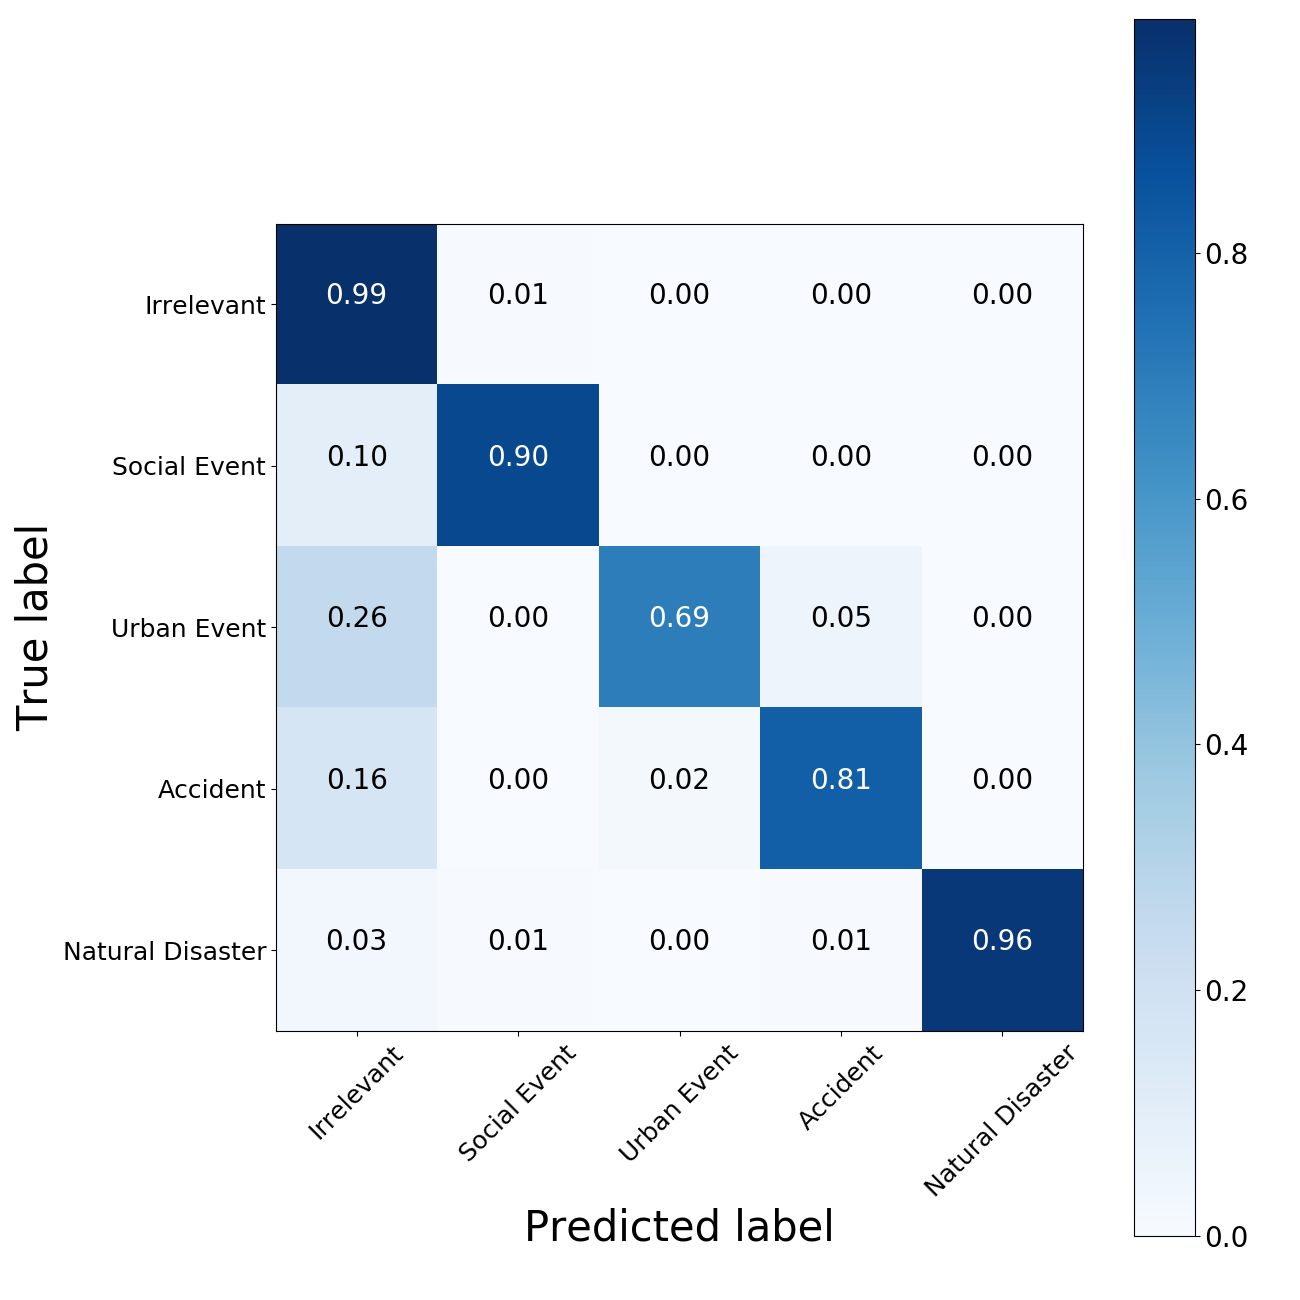
\includegraphics[width=1\linewidth]{images/confusion_matrix_rl.png}
	\label{fig:confusion_matrix_rl}
\end{figure}

\begin{figure}[!htb]
	\centering
 	  \caption{Matriz de confusão relacionada a classificação dos \textit{tweets} em eventos de exceção por meio do algoritmo Árvore de Decisão}
		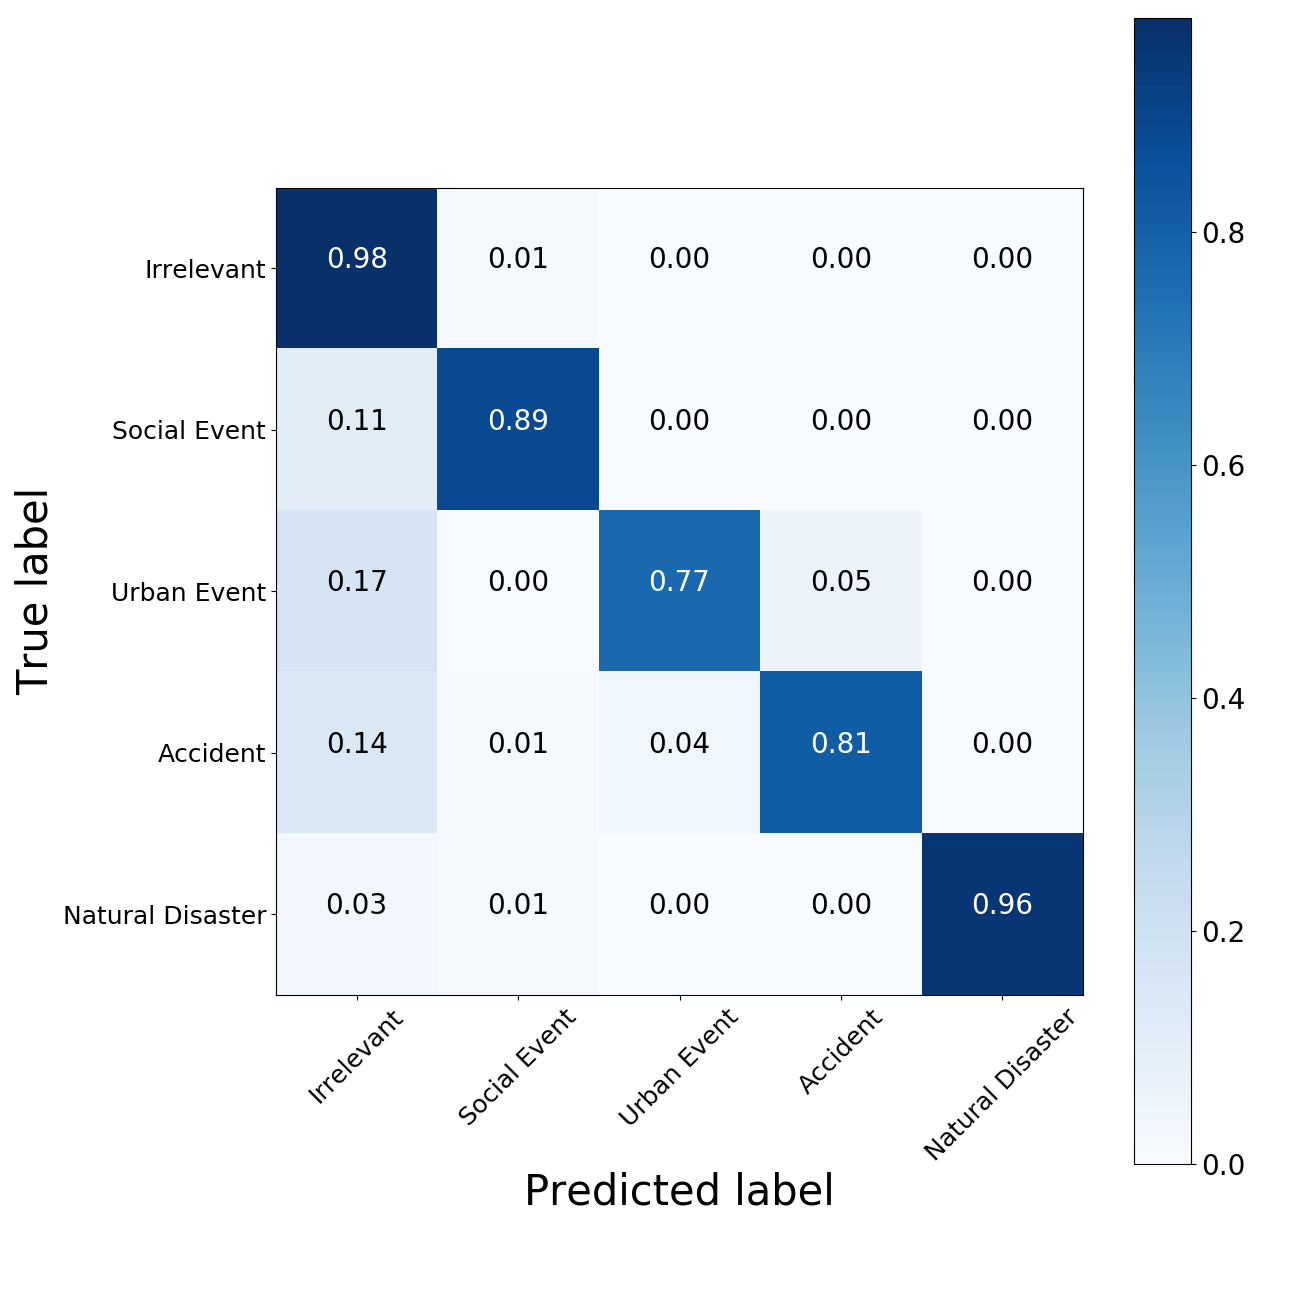
\includegraphics[width=1\linewidth]{images/confusion_matrix_dt.png}
	\label{fig:confusion_matrix_dt}
\end{figure}

\begin{figure}[!htb]
	\centering
 	  \caption{Matriz de confusão relacionada a classificação dos \textit{tweets} em eventos de exceção por meio do algoritmo \textit{Multinomial Naive Bayes}}
		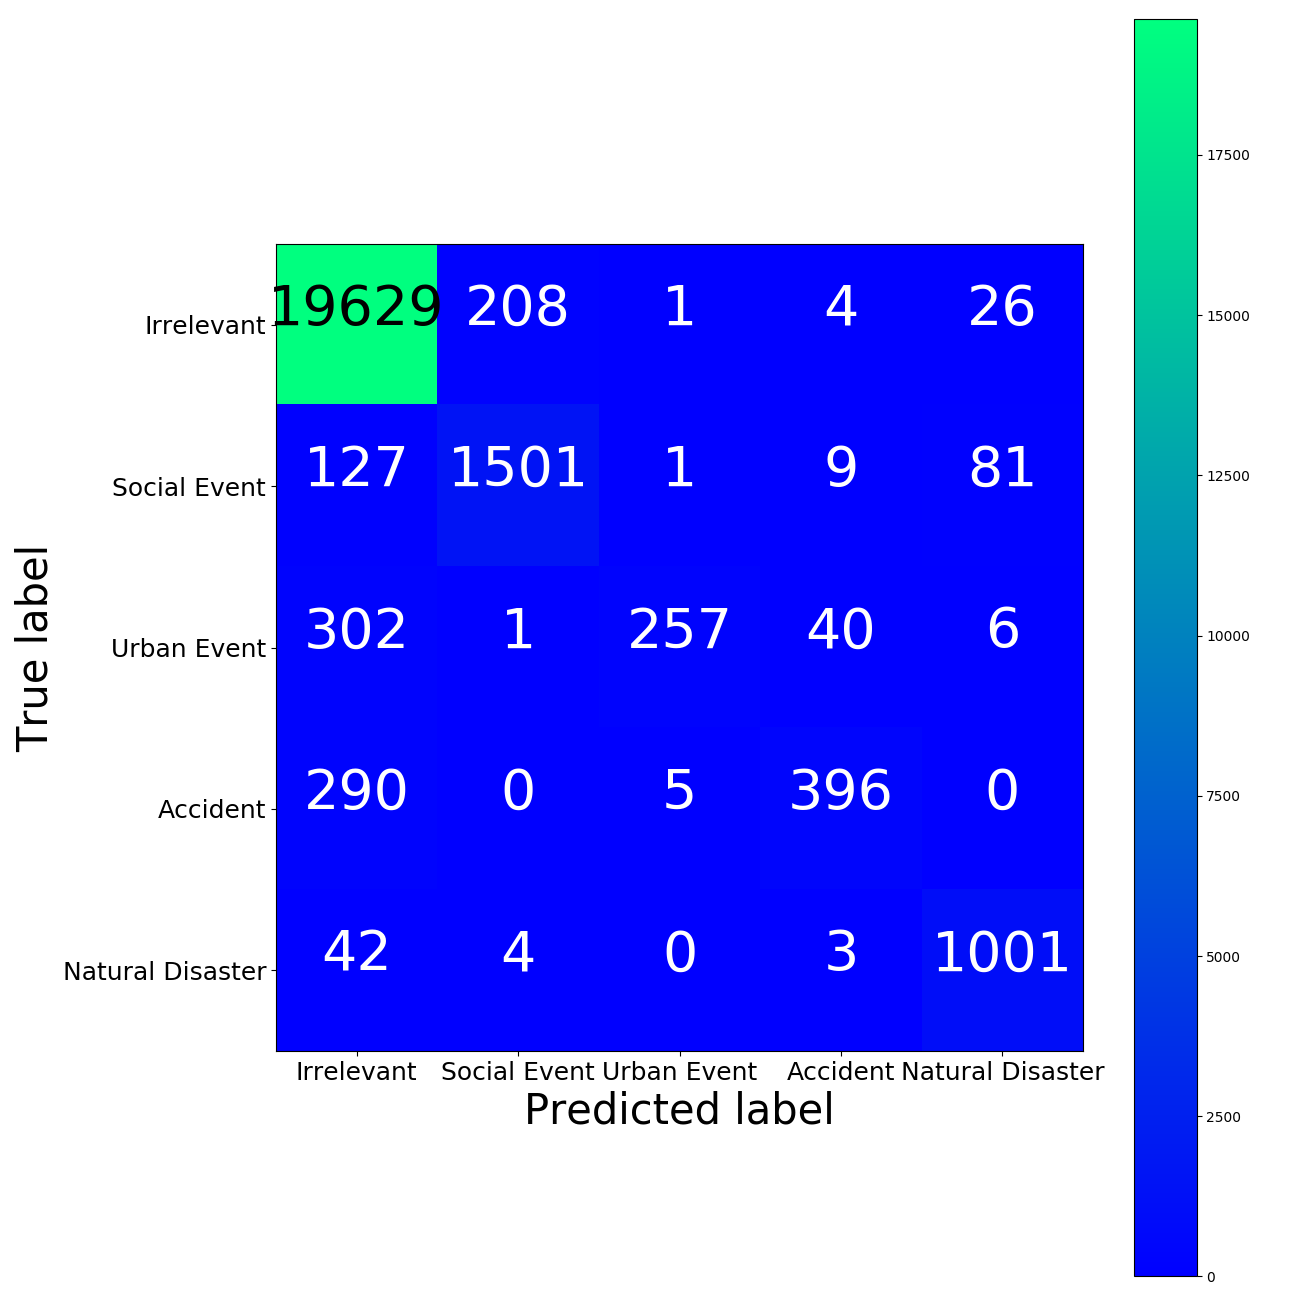
\includegraphics[width=1\linewidth]{images/confusion_matrix_mnb.png}
	\label{fig:confusion_matrix_mnb}
\end{figure}

\begin{figure}[!htb]
	\centering
 	  \caption{Matriz de confusão relacionada a classificação dos \textit{tweets} em eventos de exceção por meio do algoritmo \textit{Gaussian Naive Bayes}}
		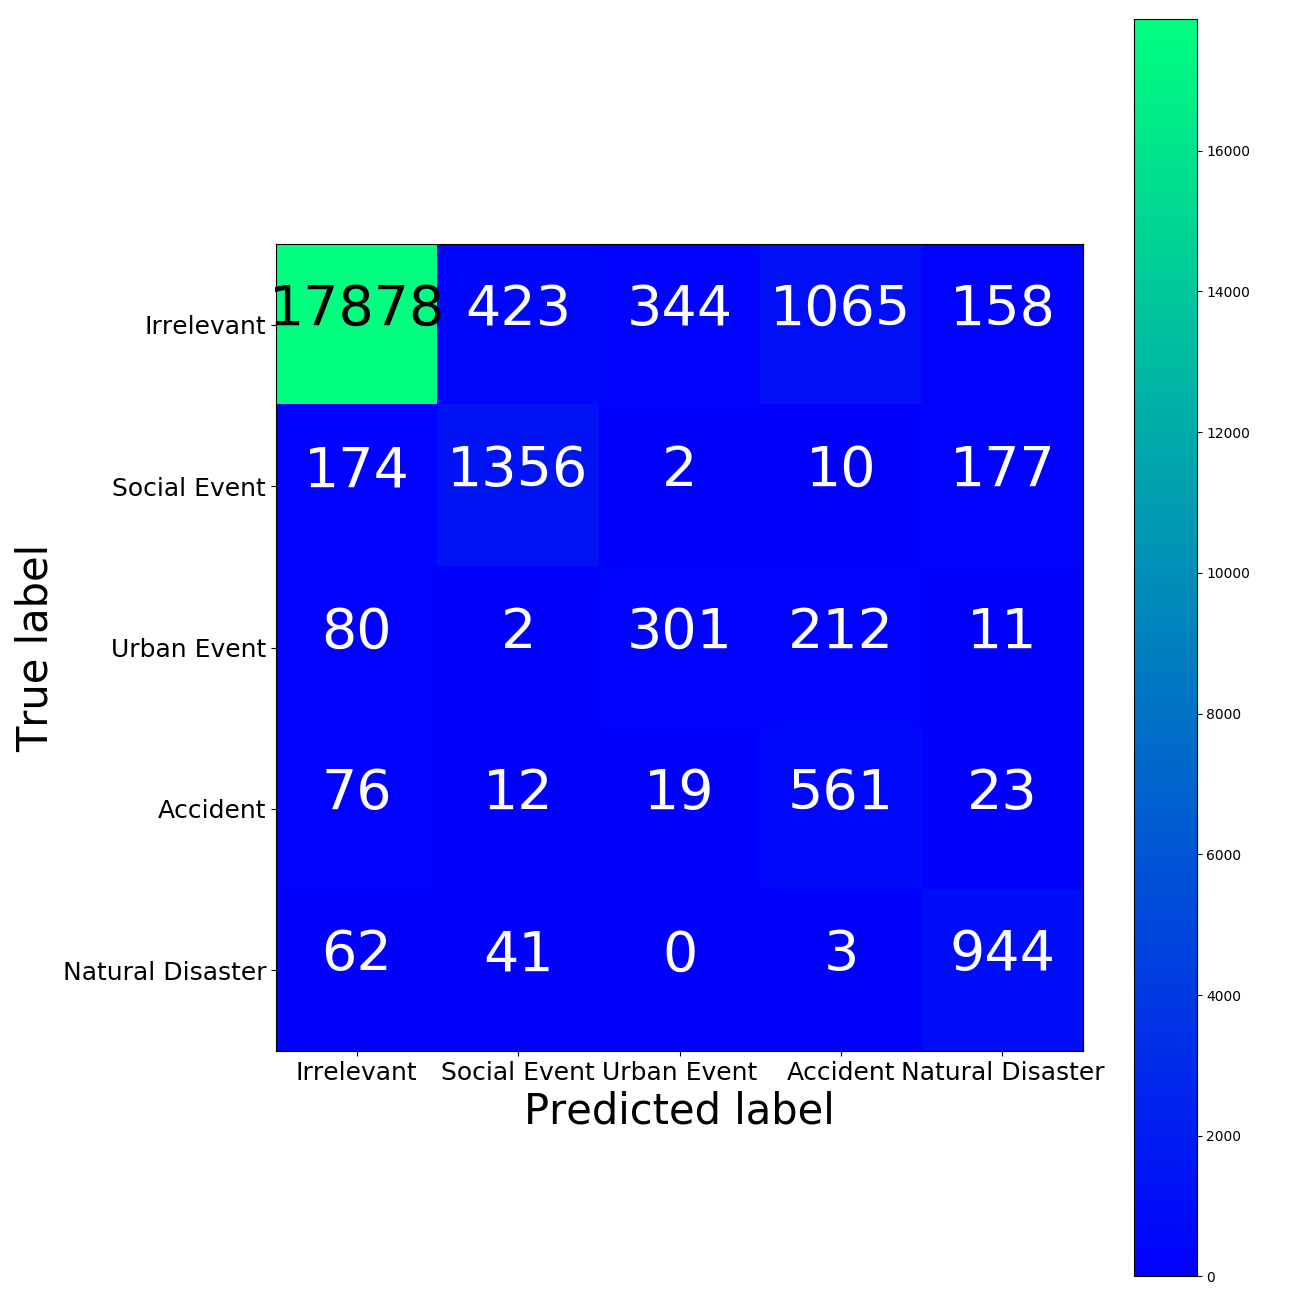
\includegraphics[width=1\linewidth]{images/confusion_matrix_gnb.png}
	\label{fig:confusion_matrix_gnb}
\end{figure}

\begin{figure}[!htb]
	\centering
 	  \caption{Matriz de confusão relacionada a classificação dos \textit{tweets} em eventos de exceção por meio do algoritmo Florestas Aleatórias}
		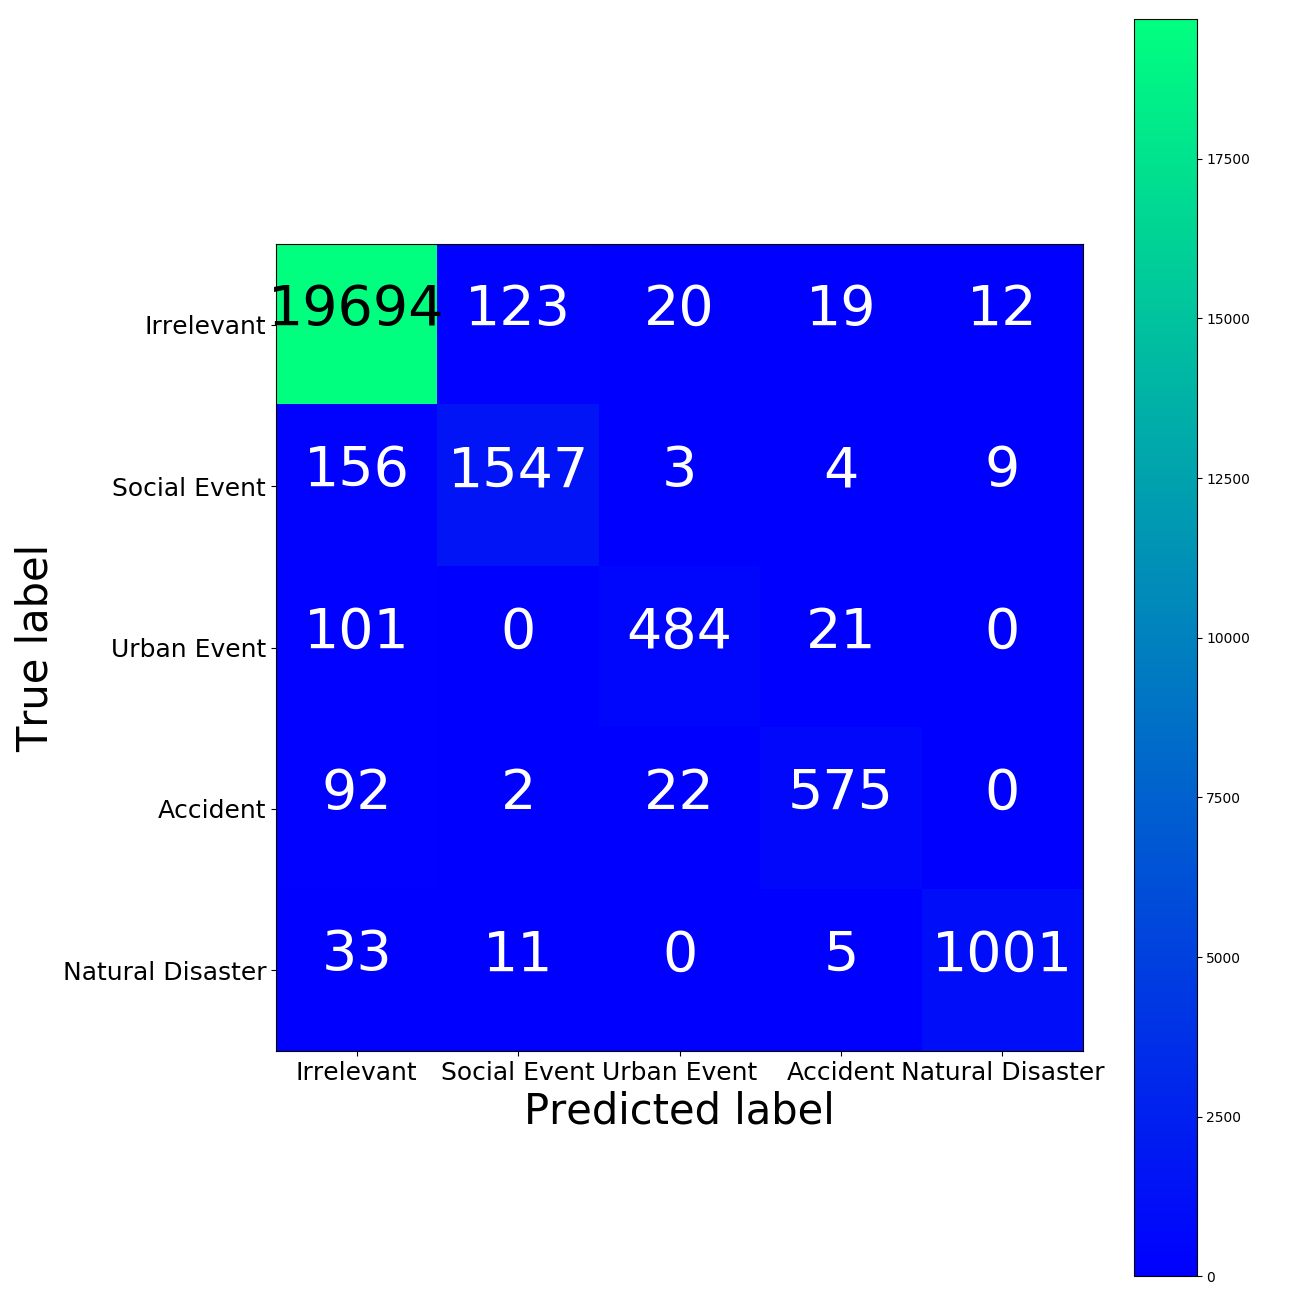
\includegraphics[width=1\linewidth]{images/confusion_matrix_rf.png}
	\label{fig:confusion_matrix_rf}
\end{figure}

\begin{figure}[!htb]
	\centering
 	  \caption{Matriz de confusão relacionada a classificação dos \textit{tweets} em eventos de exceção por meio do algoritmo Máquina de Vetores de Suporte}
		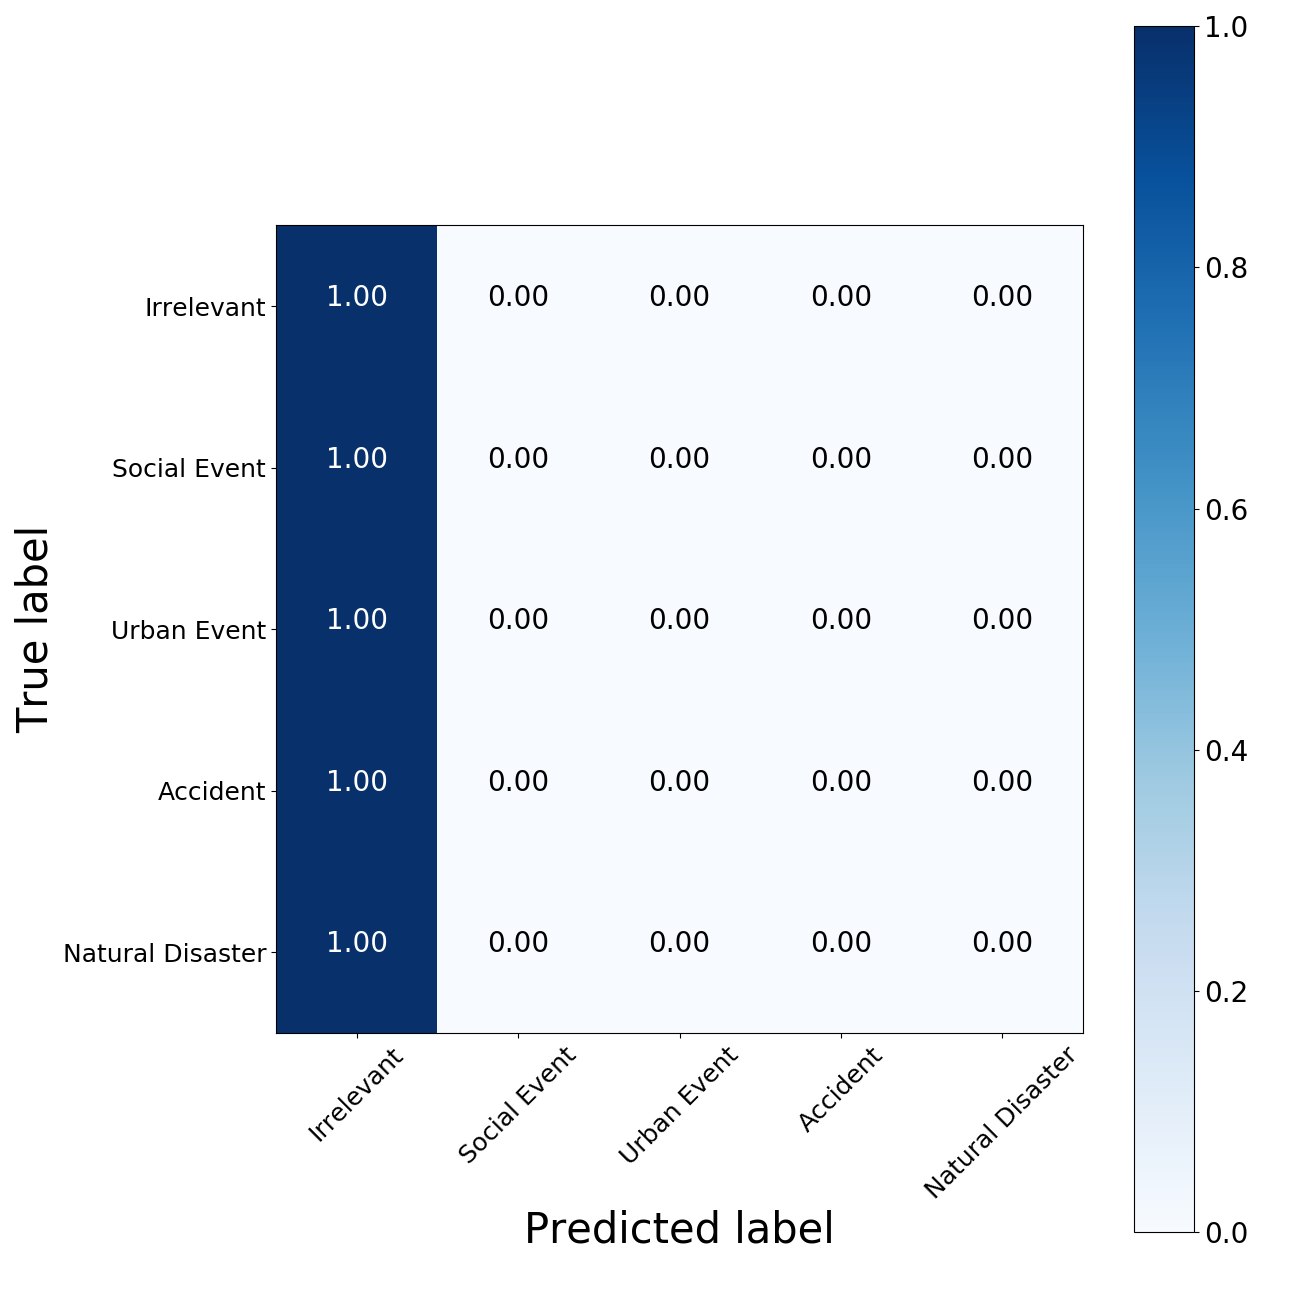
\includegraphics[width=1\linewidth]{images/confusion_matrix_svm.png}
	\label{fig:confusion_matrix_svm}
\end{figure}

\chapter{Parametrizações dos algoritmos}
\label{apendiceF}

\section{Árvore de Decisão}\footnote{Descrições das parametrização adaptadas com base em:\url{http://scikit-learn.org/stable/modules/generated/sklearn.tree.DecisionTreeClassifier.html}. Acessado em 08 de outubro de 2018.}
\begin{itemize}
\item \textit{criterion} --- $string$, opcional ($default=$\textit{``gini''}) --- Parâmetro responsável por definir a função que mede a qualidade da divisão da árvore de decisão. Os valores suportados são $gini$ para a \textit{impureza Gini} e $entropy$ para o \textit{ganho de informação}.
\item \textit{splitter} --- $string,$ opcional ($default=$\textit{``best''}) --- Parâmetro responsável por definir a estratégia usada para escolher a divisão em cada nó. As estratégias suportadas são $best$ para escolher a melhor divisão e $random$ para escolher a melhor divisão aleatoriamente.
\item \textit{max\_depth} --- $int$ ou $None$, opcional ($default=None$) --- Parâmetro responsável por definir a profundidade máxima da árvore. Se definido como $None$, os nós são expandidos até que todas as folhas fiquem puras ou até que todas as folhas contenham menos amostras que $min\_samples\_split$.
\item \textit{min\_samples\_split} --- $int$, $float$, opcional ($default=2$) --- Parâmetro responsável por definir o número mínimo de amostras necessárias para dividir um nó interno.
\item \textit{min\_samples\_leaf} --- $int$, $float$, opcional ($default=1$) --- Parâmetro responsável por definir o número mínimo de amostras necessárias em um nó folha. Um ponto de divisão em qualquer profundidade só será considerado se deixar pelo menos $min\_samples\_leaf$ amostras de treinamento em cada uma das ramificações esquerda e direita. Isso pode ter o efeito de suavizar o modelo, especialmente na regressão.
\item \textit{min\_weight\_fraction\_leaf} --- $float$, opcional ($default=0.$) --- Parâmetro responsável por definir a fração ponderada mínima da soma total de pesos (de todas as amostras de entrada) necessária para estar em um nó folha. As amostras têm peso igual quando \textit{sample\_weight} não é fornecido.
\item \textit{max\_features} --- $int$, $float$, $string$ ou $None$, opcional ($default=None$) --- Parâmetro responsável por definir o número de \textit{features} (características) a serem consideradas ao procurar a melhor divisão. A procura por uma divisão não é interrompida até que pelo menos uma partição válida das amostras de nó seja localizada, mesmo que seja necessário inspecionar do que mais de \textit{max\_features} características.
\item \textit{random\_state} --- $int$, $RandomState instance$ ou $None$, opcional ($default=None$) --- Parâmetro responsável por determinar a estratégia de geração de número aleatórios. Se definido como $RandomState$, $random\_state$ será o gerador de números aleatórios; se $None$ o gerador de números aleatórios é a instância $RandomState$ usada por $np.random$.
\item \textit{max\_leaf\_nodes} --- $int$ ou $None$, opcional ($default=None$) --- Parâmetro responsável por gerar uma árvore com o máximo número de nós folhas, usando a estratégia \textit{best-first}.
Os melhores (\textit{best}) nós são os definidos como redução relativa a impureza. Caso o parâmetro seja definido como $None$ então o número máximo de nós folhas será ilimitado. 
\item \textit{min\_impurity\_decrease} --- $float$, opcional ($default=0.$) --- Parâmetro responsável por definir que um nó será dividido se essa divisão induzir uma diminuição da impureza maior ou igual a esse valor.
\item \textit{class\_weight} --- $dict$, $list$ de $dict$, ``$balanced$'', $None$, $default=None$ --- Parâmetro responsável por associar ponderação as classes, no seguinte formato: ``${class\_label: weight}$''. Caso não haja valores para esse parâmetro, supõem-se que todos as classes possuam o mesmo peso. 
\item \textit{presort} --- $bool$, opcional ($default=False$) --- Se o valor desse parâmetro é igual a $true$ é realizada uma pré-ordenação dos dados, o que acelera encontrar as melhores divisões das árvores de decisão no processo de ajuste. Ao habilitar esse parâmetro, a velocidade do processo de treinamento de um grande volume de dados  é reduzida. Por outro lado, habilitar esse parâmetro em alguns casos pode acelerar o processo de treinamento, como quando há pequenos conjuntos de dados, ou, restrição quanto a profundidade da árvore de decisão.
\end{itemize}

\section{Floresta Aleatória}\footnote{Descrições das parametrização adaptadas com base em:\url{http://scikit-learn.org/stable/modules/generated/sklearn.ensemble.RandomForestClassifier.html}. Acessado em 08 de outubro de 2018.}

\begin{itemize}
\item \textit{n\_estimators} --- $integer$, opcional ($default=100$) --- Parâmetro responsável pelo número de árvores na floresta.
\item \textit{criterion} --- $string$, opcional ($default=$\textit{``gini''}) --- Parâmetro responsável por definir a função que mede a qualidade da divisão da árvore de decisão. Os valores suportados são $gini$ para a \textit{impureza Gini} e $entropy$ para o \textit{ganho de informação}.
\item \textit{max\_depth} --- $int$ ou $None$, opcional ($default=None$) --- Parâmetro responsável por definir a profundidade máxima da árvore. Se definido como $None$, os nós são expandidos até que todas as folhas fiquem puras ou até que todas as folhas contenham menos amostras que $min\_samples\_split$.
\item \textit{min\_samples\_split} --- $int$, $float$, opcional ($default=2$) --- Parâmetro responsável por definir o número mínimo de amostras necessárias para dividir um nó interno.
\item \textit{min\_samples\_leaf} --- $int$, $float$, opcional ($default=1$) --- Parâmetro responsável por definir o número mínimo de amostras necessárias em um nó folha. Um ponto de divisão em qualquer profundidade só será considerado se deixar pelo menos $min\_samples\_leaf$ amostras de treinamento em cada uma das ramificações esquerda e direita. Isso pode ter o efeito de suavizar o modelo, especialmente na regressão.
\item \textit{min\_weight\_fraction\_leaf} --- $float$, opcional ($default=0.$) --- Parâmetro responsável por definir a fração ponderada mínima da soma total de pesos (de todas as amostras de entrada) necessária para estar em um nó folha. As amostras têm peso igual quando \textit{sample\_weight} não é fornecido.
\item \textit{max\_features} --- $int$, $float$, $string$ ou $None$, opcional ($default=None$) --- Parâmetro responsável por definir o número de \textit{features} (características) a serem consideradas ao procurar a melhor divisão. A procura por uma divisão não é interrompida até que pelo menos uma partição válida das amostras de nó seja localizada, mesmo que seja necessário inspecionar do que mais de \textit{max\_features} características.
\item \textit{random\_state} --- $int$, $RandomState instance$ ou $None$, opcional ($default=None$) --- Parâmetro responsável por determinar a estratégia de geração de número aleatórios. Se definido como $RandomState$, $random\_state$ será o gerador de números aleatórios; se $None$ o gerador de números aleatórios é a instância $RandomState$ usada por $np.random$.
\item \textit{max\_leaf\_nodes} --- $int$ ou $None$, opcional ($default=None$) --- Parâmetro responsável por gerar uma árvore com o máximo número de nós folhas, usando a estratégia \textit{best-first}.
Os melhores (\textit{best}) nós são os definidos como redução relativa a impureza. Caso o parâmetro seja definido como $None$ então o número máximo de nós folhas será ilimitado. 
\item \textit{min\_impurity\_decrease} --- $float$, opcional ($default=0.$) --- Parâmetro responsável por definir que um nó será dividido se essa divisão induzir uma diminuição da impureza maior ou igual a esse valor.
\item \textit{bootstrap} --- $boolean$, opcional ($default=True$) --- Parâmetro responsável por definir se amostras de \textit{bootstrap} serão usadas ao construir árvores.
\item \textit{oob\_score} --- $boolean$, opcional ($default=False$) --- Parâmetro responsável por definir o uso de amostras \textit{out-of-bag} para estimar a precisão da generalização.
\item \textit{n\_jobs} --- $int$ ou $None$, opcional ($default=None$) --- Parâmetro responsável por definir o número de $jobs$ a serem executados em paralelo durante os processos de \textit{fit} e \textit{predict}. $None$ define 1 \textit{job} a menos que esteja em um contexto \textit{joblib.parallel\_backend}; -1 define que todos os processadores sejam usados.
\item \textit{verbose} --- $int$, opcional ($default=0$) ---
Parâmetro responsável por controlar a verbosidade durante os processos de \textit{fit} e \textit{predict}.
\item \textit{warm\_start} --- $bool$, opcional ($default=False$) --- Parâmetro que
quando definido como $True$ reutiliza a solução da chamada anterior no processo de \textit{fit} e adiciona mais estimadores ao \textit{ensemble}, caso contrário, apenas aplica o processo de \textit{fit} a toda uma nova floresta.
\item \textit{class\_weight} --- $dict$, $list$ de $dict$, ``$balanced$'', $None$, $default=None$ --- Parâmetro responsável por associar ponderação as classes, no seguinte formato: ``${class\_label: weight}$''. Caso não haja valores para esse parâmetro, supõem-se que todos as classes possuam o mesmo peso. 
\item \textit{presort} --- $bool$, opcional ($default=False$) --- Se o valor desse parâmetro é igual a $true$ é realizada uma pré-ordenação dos dados, o que acelera encontrar as melhores divisões das árvores de decisão no processo de ajuste. Ao habilitar esse parâmetro, a velocidade do processo de treinamento de um grande volume de dados  é reduzida. Por outro lado, habilitar esse parâmetro em alguns casos pode acelerar o processo de treinamento, como quando há pequenos conjuntos de dados, ou, restrição quanto a profundidade da árvore de decisão.
\end{itemize}

\section{K-ésimo Vizinho mais Próximo}\footnote{Descrições das parametrização adaptadas com base em:\url{http://scikit-learn.org/stable/modules/generated/sklearn.neighbors.KNeighborsClassifier.html}. Acessado em 08 de outubro de 2018.}

\begin{itemize}

\item \textit{n\_neighbors} --- $int$, opcional ($default = 5$) --- Parâmetro responsável por definir o número padrão de \textit{neighbors} usados pelas \textit{kneighbors queries}.

\item \textit{weights} --- $str$ ou $callable$, opcional ($default = ‘uniform’$) --- Parâmetro usado para definir a função de peso usada no processo \textit{predict}. Valores possíveis: (I) $uniform$: pesos uniformes; todos os pontos em cada vizinha são ponderados igualmente; (II) $distance$: pontos de ponderação pelo inverso da suas respectivas distâncias; nesse caso, os vizinhos mais próximos de um ponto de consulta terão uma influência maior do que os vizinhos mais distantes; (III) $callable$: uma função definida pelo usuário que aceita uma matriz de distâncias e retorna uma matriz da mesma forma, contendo contém os pesos.

\item \textit{algorithm} --- $auto$, $ball\_tree$ (\textit{BallTree}), $kd\_tree$ (\textit{KDTree}), $brute$ (pesquisa por força bruta), opcional ($default = ‘auto’$) --- Parâmetro responsável por definir algoritmo utilizado para calcular os vizinhos mais próximos. O valor padrão tentará decidir o algoritmo mais apropriado com base nos valores passados para o método \textit{fit}. Em case de dados esparsos no processo de ajuste esse parâmetro é ignorado e usado a opção $brute$ por padrão.

\item \textit{leaf\_size} --- $int$, opcional ($default = 30$) --- Parâmetro responsável por definir o tamanho da folha passado para o \textit{BallTree} ou \textit{KDTree}. Isso pode afetar a velocidade da construção e consulta, bem como a memória necessária para armazenar a árvore. O valor ideal depende da natureza do problema.

\item \textit{p} --- $integer$, opcional ($default = 2$) --- Parâmetro de potência para a métrica \textit{Minkowski}. Quando p = 1, isso equivale a usar \textit{manhattan\_distance} ($l1$) e \textit{euclidean\_distance} ($l2$) para p = 2. Para \textit{p} arbitrário, \textit{minkowski\_distance} ($l\_p$) é usado.

\item \textit{metric} --- $string$ ou $callable$, opcional ($default = ‘minkowski’$) --- Parâmetro responsável por definir a distância métrica para usar na árvore. A métrica padrão é \textit{minkowski} e com $p = 2$ é equivalente à métrica euclidiana padrão. 

\item \textit{n\_jobs} --- $int$ ou $None$, opcional ($default = None$) --- Parâmetro responsável por definir o número de $jobs$ a serem executados em paralelo durante os processos de \textit{fit} e \textit{predict}. $None$ define 1 \textit{job} a menos que esteja em um contexto \textit{joblib.parallel\_backend}; -1 define que todos os processadores sejam usados.
\end{itemize}

\section{Máquina de Vetores de Suporte}\footnote{Descrições das parametrização adaptadas com base em:\url{http://scikit-learn.org/stable/modules/generated/sklearn.svm.SVC.html\#sklearn.svm.SVC}. Acessado em 08 de outubro de 2018.}

\begin{itemize}
\item \textit{C} --- $float$, opcional ($default=1.0$)
 --- Parâmetro de \textit{penalidade C} do termo de erro.
 
 \item \textit{kernel} --- $string$, opcional ($default='rbf'$) --- Parâmetro responsável por especificar o tipo de \textit{kernel} a ser usado no algoritmo. Pode ser $linear$, $poli$, $rbf$, $sigmoid$, $precomputed$ ou $callable$.

\item \textit{degree} --- $int$, opcional ($default=3$) --- Parâmetro responsável por definir a \textit{polynomial kernel function} ($poly$). Ignorado por todos os 
outros \textit{kernels}.

\item \textit{gamma} --- $float$, opcional ($default='auto'$) --- Parâmetro responsável por definir o coeficiente de \textit{Kernel} para $rbf$, $poly$ e $sigmoid$.

\item \textit{coef0} --- $float$, opcional ($default=0.0$) --- Parâmetro responsável por definir o termo independente na função \textit{kernel}. É significativo apenas para $poli$ e $sigmoid$.

\item \textit{shrinking} --- $boolean$, opcional ($default=True$) --- Parâmetro responsável por definir o uso da heurística $shrinking$.

\item \textit{probability} --- $boolean$, opcional ($default=False$) --- Parâmetro responsável por definir o uso de estimativas de probabilidade, o qual deve ser ativado antes do processo de $fit$ (implica em perda de desempenho).

\item \textit{tol} --- $float$, opcional ($default=1e-3$) --- Parâmetro responsável por definir a tolerância ao critério de parada.

\item \textit{cache\_size} --- $float$, opcional --- Parâmetro responsável por definir o tamanho do cache do \textit{kernel} (em MB).

\item \textit{class\_weight} --- $dict$, $balanced$, optional ($default = None$) --- Parâmetro responsável  por definir o parâmetro C da classe $i$ para $class\_weight[i]*C$ para o \textit{SVC}.

\item \textit{verbose} --- $bool$, ($default = False$) --- Parâmetro responsável por habilitar a saída detalhada.

\item \textit{max\_iter} --- $int$, opcional ($default=-1$) --- Parâmetro responsável por definir um limite rígido em iterações no \textit{solver}, ou -1 para sem limite.

\item \textit{decision\_function\_shape} --- $ovo$, $ovr$, ($default='ovr'$) --- Parâmetro responsável por definir se deve retornar uma função de decisão \textit{one-vs-rest} ($ovr$) ou a função de decisão original \textit{one-vs-one}.

\item \textit{random\_state} --- $int$, $RandomState instance$ ou $None$, opcional ($default=None$) --- Parâmetro responsável por determinar a estratégia de geração de número aleatórios. Se definido como $RandomState$, $random\_state$ será o gerador de números aleatórios; se $None$ o gerador de números aleatórios é a instância $RandomState$ usada por $np.random$.

\end{itemize}

%decision_function_shape : ‘ovo’, ‘ovr’, default=’ovr’
%Whether to return a one-vs-rest (‘ovr’) decision function of shape (n_samples, n_classes) as all other classifiers, or the original one-vs-one (‘ovo’) decision function of libsvm which has shape (n_samples, n_classes * (n_classes - 1) / 2). However, one-vs-one (‘ovo’) is always used as multi-class strategy.
%Changed in version 0.19: decision_function_shape is ‘ovr’ by default.
%New in version 0.17: decision_function_shape=’ovr’ is recommended.
%Changed in version 0.17: Deprecated decision_function_shape=’ovo’ and None.
%random_state : int, RandomState instance or None, optional (default=None)
%The seed of the pseudo random number generator used when shuffling the data for probability estimates. If int, random_state is the seed used by the random number generator; If RandomState instance, random_state is the random number generator; If None, the random number generator is the RandomState instance used by np.random.

\section{Naive Bayes}\footnote{Descrições das parametrização adaptadas com base em:\url{http://scikit-learn.org/stable/modules/generated/sklearn.neighbors.KNeighborsClassifier.html}. Acessado em 08 de outubro de 2018.}

\section{Redes Neurais}\footnote{Descrições das parametrização adaptadas com base em:\url{http://scikit-learn.org/stable/modules/generated/sklearn.neighbors.KNeighborsClassifier.html}. Acessado em 08 de outubro de 2018.}

\section{Regressão Logística}\footnote{Descrições das parametrização adaptadas com base em:\url{http://scikit-learn.org/stable/modules/generated/sklearn.neighbors.KNeighborsClassifier.html}. Acessado em 08 de outubro de 2018.}

\end{apendicesenv}
\end{document}
